% ============================================================
%  MAIN MANUSCRIPT
%  "How does correlation relate to causation"
%  Author: Yaohui Ding
%
%  Numbered snapshots of this manuscript's earlier lineage (v1-v4) live in
%  versions/; this file is the current, versionless working copy.
% ============================================================

\documentclass[12pt]{article}

\usepackage[letterpaper,top=2cm,bottom=2cm,left=2.54cm,right=2.54cm,marginparwidth=1.75cm]{geometry}
\usepackage{amsmath}
\usepackage{amssymb}
\usepackage{graphicx}
\usepackage[colorlinks=true, allcolors=blue]{hyperref}
\usepackage{comment}
\usepackage{xcolor}
\usepackage[font=small]{caption} % captions smaller than 12pt body text
                                  % (standard convention), applies to all
                                  % figures project-wide
\usepackage{float}
\usepackage{subcaption}

\newlength{\diagcolht} % diagram+matrices column height, matched to a panel's
\newlength{\cellwd}    % per-cell width, 3-column tabulars (Fig 3+)
\newlength{\rowwd}     % = 3*\cellwd + 12pt, full row width (for the colorbar)
\newlength{\labxshiftB} % xshift for column-2/3 panel labels
\usepackage{tikz}
\usetikzlibrary{arrows.meta, positioning}
\usepackage[natbibapa]{apacite}
\usepackage{standalone}
\usepackage{cancel} % for \cancel{} diagonal strikethrough (Appendix D reducibility subsection)
\renewcommand{\CancelColor}{\color{red}} % make \cancel{} strikethrough lines red
\usepackage{bibunits} % gives each \input'd appendix its own local reference list



% ----------------------------
% PARAMETERS
% ----------------------------
\def\a{1.2 cm}          % triangle size
\def\nodeSize{0.7}     % node diameter (cm)
\def\selfLoopR{0.5*\nodeSize cm}

% ----------------------------
% SELF-LOOPS
% ----------------------------
\newcommand{\selfloop}[2]{%
% #1 = node, #2 = position (1=left, 2=right, 3=top)

\ifnum#2=1
\draw[->]
({- \a},{-\selfLoopR})
arc[start angle=0,end angle=-270,radius=\selfLoopR];
\fi

% Loop for node 2
\ifnum#2=2
\draw[->]
({ \a},{-\selfLoopR})
arc[start angle=-180,end angle=90,radius=\selfLoopR];
\fi

% Loop for node 3
\ifnum#2=3
\draw[->]
({0},{sqrt(3) * \a +\selfLoopR})
arc[start angle=180,end angle=-90,radius=\selfLoopR];
\fi
}








\setlength{\parindent}{0pt}

\title{How does correlation relate to causation: seven insights from an analytic relationship between the two}

\author{Yaohui Ding}

\begin{document}

\maketitle

% ============================================================
%  ABSTRACT
% ============================================================


\section*{Abstract}

``Correlation does not imply causation,'' the adage warns.
But how does correlation relate to causation?
For linear stochastic dynamical systems driven by white
noise, a widely used class of models across the natural and
social sciences, the question has an exact answer.
At steady state, correlation (more precisely covariance) and causation are linked by the
Lyapunov equation. From this equation we derive closed-form expressions for pairwise correlation coefficients as explicit
functions of the causal parameters and noise variances. We analyze these expressions for nine network topologies and unpack seven insights regarding the relationship between correlation and causation. For instance, we illustrate through some examples that causation is transitive, while correlation is not; and that the mapping from causation to correlation is generally many-to-one. The formulae also reveal that the covariance
between any two variables is a linear combination of the
noise variances, with weights that are
highly nonlinear functions of the causal parameters. This is one of the reasons that
the relationship between correlation and causation resists simple
intuition. We show that the formulae from the
fully connected three-node network serve as the ``master
formulae'' for $3\times3$ networks, because of the structural
symmetry of its topology, and can be reduced to the formulae for
every sparser three-node network as causal connections are
set to zero. Finally, we note that the Lyapunov equation is a unifying  mathematical object for causal modeling
frameworks such as Granger causality and dynamic causal modeling, with additive white noise assumption. \\

\noindent\textbf{Keywords:} correlation, causation, linear stochastic dynamical system, Lyapunov equation




% \newpage

% ============================================================
%  INTRODUCTION
%  For: "How does correlation relate to causation"
%  Author: Yaohui Ding
% ============================================================

\clearpage
\section*{Introduction}

``Correlation does not imply causation'' is one of the most
repeated mantras in science, taught early and invoked often.
Yet the mantra, for all its wisdom, leaves a deeper question
unanswered. If correlation does not imply causation, how
exactly do they relate to each other?
Intuitively, a correlation between two variables can arise because one
directly causes the other, both are driven by a common cause, influence is relayed through intermediary variables, or some
combination of all three.

Quantifying the relationship between correlation and causation is a problem that is at least a century old.
Sewall Wright, in a landmark paper titled \textit{Correlation
and Causation} \citep{Wright1921}, gave an early rigorous answer to this problem:
the correlation between any two variables equals the sum of
the products of the path coefficients along each path, over
all directed paths in a causal diagram connecting these two
variables.
Wright later developed this idea, which he called the
\textit{tracing rule}, into the \textit{method of path
coefficients} \citep{Wright1934}.
But the method has a structural limitation. It applies only
to directed acyclic graphs, in which the causal influences
from one variable to another flow only in one direction and
never loop back (i.e., no reciprocal interaction).
Wright saw the limitation clearly and returned to it nearly
four decades later.
He attempted to accommodate reciprocal interaction and
feedback (self-loop) through lagged models and simultaneous
equations \citep{Wright1960}, yet without
arriving at a satisfying closed-form analytic solution for
this problem.

Surprisingly, for dynamical systems with reciprocal
interaction and feedback --- the norm rather than the
exception in biology, neuroscience, and the social sciences
--- the problem of determining, precisely and analytically,
the pattern of correlation from a
known causal structure remained open
for more than half of a century (\hyperref[app:appE]{Appendix~E}) after \citet{Wright1960}.
In the last few years, work in algebraic statistics has
generalized Wright's method of path coefficients (or
\textit{tracing rule}) to a \textit{trek rule}
\citep{VarandoHansen2020, HansenTrek2025} for dynamic causal networks with reciprocal
interaction and feedback, which is referred to as graphical continuous Lyapunov models in this line of work. Although the \textit{trek rule} is a powerful tool for studying the reachability, conditional independence, and learning of causal networks, it involves evaluating convergent but infinite power series when calculating the covariance of a pair of variables of interest from the network.


% ------------------------------------------------------------
\subsection*{The Present Work}
% ------------------------------------------------------------
Our current study takes a complementary approach to that of \citet{VarandoHansen2020}. Similar to their approach, we model $n$ interacting variables as a linear stochastic dynamical system with additive white noise. It is known in the literature that, at steady state, the patterns of causation and patterns of correlation (more precisely covariance) of such kind of system are related to each other via the Lyapunov equation
\citep{Lyapunov1892, Pavliotis2014, AstromMurray2021}. We solve the Lyapunov equation symbolically through a combination of the half-vectorization and Kronecker product techniques and express every
pairwise correlation coefficient $\rho_{ij}$ as a ratio of elementary functions (polynomials and square root) of the causal parameters and
noise variances --- for networks of arbitrary sizes. However, because the general formula is difficult to interpret
for large networks, we analyze it explicitly for nine
network topologies (Figure~\ref{fig:schematic_network_topo}).
The simplest is a two-node network (\textit{dyad}), in
which two variables influence each other reciprocally.
The remaining eight topologies are three-node networks. Three of these are the classic acyclic motifs in the literature of causal
reasoning \citep{Pearl2009}: the \textit{confounder}, in
which a common driver causally influences two otherwise unconnected
variables; the \textit{mediator}, in which causal influence is
relayed through an intermediary variable; and the \textit{collider},
in which two independent variables drive a common
target. The other three-node networks all have cycles. For example, a
\textit{two-way mediator} network has mediating influence
running in both directions that forms two \textit{2-cycles}. In contrast, in the \textit{3-cycle} example, the three variables form a \textit{3-cycle}.
Finally, the
\textit{fully connected} network, in which every variable
influences every other, is the most general three-node topology
and subsumes all the other $3\times3$ networks.
We emphasize that triadic architectures are prevalent in the
scientific literature --- for example, the triple-network
model in neuroscience \citep{Menon2011, Menon2023}, which posits three
interacting large-scale brain networks to explain a range of
psychopathologies \citep{Kaiser2015, MenonPalaniyappanSupekar2023, LiEtAl2023}. Thus, the analytic results and insights we derive in the current study may prove useful when reasoning about the relationship between correlation and causation in these triadic models, provided that they make similar modeling assumptions.


\begin{figure}[H]
\centering

% -------- Row 1: Dyad | Confounder | Collider --------

% Dyad
\begin{subfigure}[b]{0.32\textwidth}
\centering
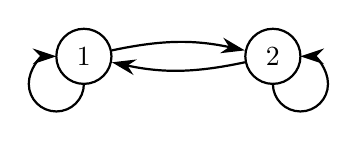
\begin{tikzpicture}[
    thick,
    >={Stealth[length=3mm,width=2mm]},
    every node/.style={circle, draw, minimum size=\nodeSize cm}
]
\node (1) at (-\a,0) {1};
\node (2) at (\a,0) {2};
\draw[->] (1) to[bend left=12] (2);
\draw[->] (2) to[bend left=12] (1);
\selfloop{1}{1}
\selfloop{2}{2}
\end{tikzpicture}
\caption{Dyad}
\end{subfigure}
\hfill
%
% Confounder
\begin{subfigure}[b]{0.32\textwidth}
\centering
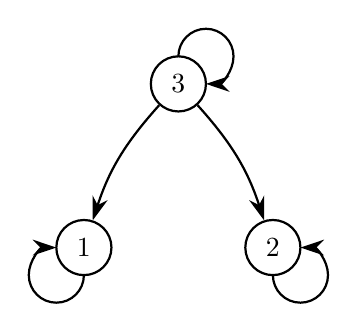
\begin{tikzpicture}[
    thick,
    >={Stealth[length=3mm,width=2mm]},
    every node/.style={circle, draw, minimum size=\nodeSize cm}
]
\node (1) at (-\a,0) {1};
\node (2) at (\a,0) {2};
\node (3) at (0,{sqrt(3)*\a}) {3};
\draw[->] (3) to[bend right=12] (1);
\draw[->] (3) to[bend left=12] (2);
\selfloop{1}{1}
\selfloop{2}{2}
\selfloop{3}{3}
\end{tikzpicture}
\caption{Confounder}
\end{subfigure}
\hfill
%
% Collider
\begin{subfigure}[b]{0.32\textwidth}
\centering
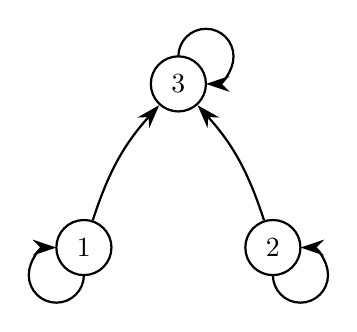
\begin{tikzpicture}[
    thick,
    >={Stealth[length=3mm,width=2mm]},
    every node/.style={circle, draw, minimum size=\nodeSize cm}
]
\node (1) at (-\a,0) {1};
\node (2) at (\a,0) {2};
\node (3) at (0,{sqrt(3)*\a}) {3};
\draw[->] (1) to[bend left=12] (3);
\draw[->] (2) to[bend right=12] (3);
\selfloop{1}{1}
\selfloop{2}{2}
\selfloop{3}{3}
\end{tikzpicture}
\caption{Collider}
\end{subfigure}

\vspace{0.5cm}

% -------- Row 2: Mediator | Two-Way Mediator | 3-Cycle --------

% Mediator
\begin{subfigure}[b]{0.32\textwidth}
\centering
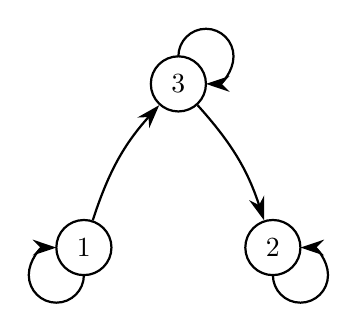
\begin{tikzpicture}[
    thick,
    >={Stealth[length=3mm,width=2mm]},
    every node/.style={circle, draw, minimum size=\nodeSize cm}
]
\node (1) at (-\a,0) {1};
\node (2) at (\a,0) {2};
\node (3) at (0,{sqrt(3)*\a}) {3};
\draw[->] (1) to[bend left=12] (3);
\draw[->] (3) to[bend left=12] (2);
\selfloop{1}{1}
\selfloop{2}{2}
\selfloop{3}{3}
\end{tikzpicture}
\caption{Mediator}
\end{subfigure}
\hfill
%
% Two-Way Mediator
\begin{subfigure}[b]{0.32\textwidth}
\centering
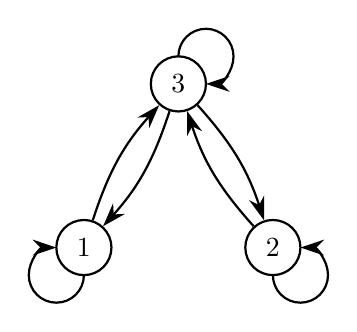
\begin{tikzpicture}[
    thick,
    >={Stealth[length=3mm,width=2mm]},
    every node/.style={circle, draw, minimum size=\nodeSize cm}
]
\node (1) at (-\a,0) {1};
\node (2) at (\a,0) {2};
\node (3) at (0,{sqrt(3)*\a}) {3};
\draw[->] (1) to[bend left=12] (3);
\draw[->] (3) to[bend left=12] (1);
\draw[->] (3) to[bend left=12] (2);
\draw[->] (2) to[bend left=12] (3);
\selfloop{1}{1}
\selfloop{2}{2}
\selfloop{3}{3}
\end{tikzpicture}
\caption{Two-Way Mediator}
\end{subfigure}
\hfill
%
% 3-Cycle
\begin{subfigure}[b]{0.32\textwidth}
\centering
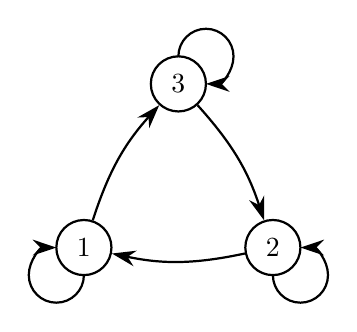
\begin{tikzpicture}[
    thick,
    >={Stealth[length=3mm,width=2mm]},
    every node/.style={circle, draw, minimum size=\nodeSize cm}
]
\node (1) at (-\a,0) {1};
\node (2) at (\a,0) {2};
\node (3) at (0,{sqrt(3)*\a}) {3};
\draw[->] (2) to[bend left=12] (1);
\draw[->] (3) to[bend left=12] (2);
\draw[->] (1) to[bend left=12] (3);
\selfloop{1}{1}
\selfloop{2}{2}
\selfloop{3}{3}
\end{tikzpicture}
\caption{3-Cycle}
\end{subfigure}

\vspace{0.5cm}

% -------- Row 3: Moderator | Coupled Drivers | Fully Connected --------

% Moderator
\begin{subfigure}[b]{0.32\textwidth}
\centering
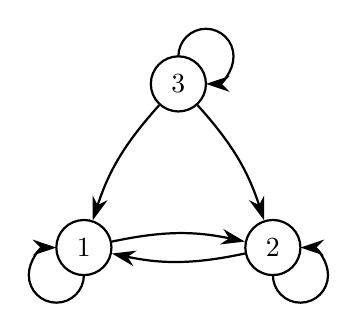
\begin{tikzpicture}[
    thick,
    >={Stealth[length=3mm,width=2mm]},
    every node/.style={circle, draw, minimum size=\nodeSize cm}
]
\node (1) at (-\a,0) {1};
\node (2) at (\a,0) {2};
\node (3) at (0,{sqrt(3)*\a}) {3};
\draw[->] (1) to[bend left=12] (2);
\draw[->] (2) to[bend left=12] (1);
\draw[->] (3) to[bend right=12] (1);
\draw[->] (3) to[bend left=12] (2);
\selfloop{1}{1}
\selfloop{2}{2}
\selfloop{3}{3}
\end{tikzpicture}
\caption{Moderator}
\end{subfigure}
\hfill
%
% Coupled Drivers
\begin{subfigure}[b]{0.32\textwidth}
\centering
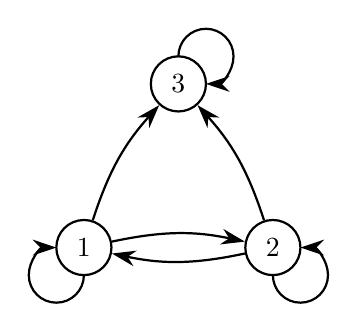
\begin{tikzpicture}[
    thick,
    >={Stealth[length=3mm,width=2mm]},
    every node/.style={circle, draw, minimum size=\nodeSize cm}
]
\node (1) at (-\a,0) {1};
\node (2) at (\a,0) {2};
\node (3) at (0,{sqrt(3)*\a}) {3};
\draw[->] (1) to[bend left=12] (2);
\draw[->] (2) to[bend left=12] (1);
\draw[->] (1) to[bend left=12] (3);
\draw[->] (2) to[bend right=12] (3);
\selfloop{1}{1}
\selfloop{2}{2}
\selfloop{3}{3}
\end{tikzpicture}
\caption{Coupled Drivers}
\end{subfigure}
\hfill
%
% Fully Connected
\begin{subfigure}[b]{0.32\textwidth}
\centering
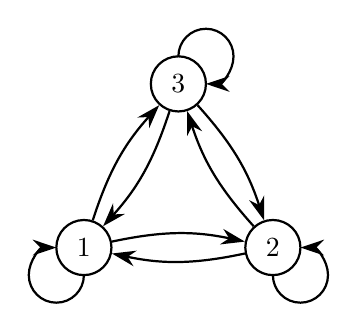
\begin{tikzpicture}[
    thick,
    >={Stealth[length=3mm,width=2mm]},
    every node/.style={circle, draw, minimum size=\nodeSize cm}
]
\node (1) at (-\a,0) {1};
\node (2) at (\a,0) {2};
\node (3) at (0,{sqrt(3)*\a}) {3};
\draw[->] (1) to[bend left=12] (2);
\draw[->] (2) to[bend left=12] (1);
\draw[->] (1) to[bend left=12] (3);
\draw[->] (3) to[bend left=12] (1);
\draw[->] (2) to[bend left=12] (3);
\draw[->] (3) to[bend left=12] (2);
\selfloop{1}{1}
\selfloop{2}{2}
\selfloop{3}{3}
\end{tikzpicture}
\caption{Fully Connected}
\end{subfigure}

\caption{Nine network topologies analyzed in the current study.}
\label{fig:schematic_network_topo}
\end{figure}

% ============================================================
%  MATHEMATICAL FRAMEWORK (short version, appears before Results)
%  For: "How does correlation relate to causation"
%  Author: Yaohui Ding
% ============================================================

\section*{Methods}

We model a system of $n$ interacting variables as a linear
stochastic dynamical system driven by additive white noise.
The pattern of causal interaction among these variables is encoded by a generally asymmetric matrix $\mathbf{A}$, whose off-diagonal entry $a_{ij}$ represents the direct causal influence of variable $j$ on
variable $i$. We assume that $\mathbf{A}$ is Hurwitz stable, i.e., all of its eigenvalues have strictly
negative real part. We further assume that the state variables ($\mathbf{X}$) are directly observed, i.e., $\mathbf{X}=\mathbf{Y}$.

\begin{equation}
\begin{aligned}
\mathbf{A} =
\begin{bmatrix}
    a_{11}  & \cdots & a_{1n} \\
     \vdots & \ddots & \vdots  \\
    a_{n1}  & \cdots & a_{nn}
\end{bmatrix},
\mathbf{\Sigma_\mathbf{Y}}=
\begin{bmatrix}
    \sigma_{11}  & \cdots & \sigma_{1n} \\
     \vdots & \ddots & \vdots  \\
    \sigma_{n1}  & \cdots & \sigma_{nn}
\end{bmatrix},
\mathbf{\Sigma_\mathbf{W}} =
\begin{bmatrix}
    \sigma_{W_1}  & \cdots & 0 \\
     \vdots & \ddots & \vdots  \\
    0  & \cdots & \sigma_{W_n}
\end{bmatrix}
\end{aligned}
\label{eq:nByn_network_mf}
\end{equation}
From these assumptions, we derive in
\hyperref[app:appA]{Appendix~A} that the steady-state
covariance matrix $\mathbf{\Sigma}_Y$ satisfies the
continuous-time Lyapunov equation
\begin{equation}
\mathbf{A}\,\mathbf{\Sigma}_Y
+ \mathbf{\Sigma}_Y\,\mathbf{A}^T
+ \mathbf{\Sigma}_W = \mathbf{0}.
\label{eq:lyapunov_mf}
\end{equation}
where $\mathbf{\Sigma}_W$ is the covariance matrix of the additive white noise, assumed to be diagonal. To solve equation~(\ref{eq:lyapunov_mf}) for a
network of arbitrary size $N$, we apply the vectorization
($\operatorname{vec}(\cdot)$) and Kronecker product ($\otimes$)
techniques (\hyperref[app:appB]{Appendix~B}) to it, which gives us
\begin{equation}
(\mathbf{I}\otimes\mathbf{A}+\mathbf{A}\otimes\mathbf{I})\,
\mathrm{vec} \mathbf{\Sigma}_Y
= -\mathrm{vec} \mathbf{\Sigma}_W,
\label{eq:lyapunov_vec_results}
\end{equation}
whose unique solution (guaranteed to exist when $\mathbf{A}$ is Hurwitz
stable) is
\begin{equation}
\mathrm{vec}\mathbf{\Sigma}_Y =
-(\mathbf{I}\otimes\mathbf{A}+\mathbf{A}\otimes\mathbf{I})^{-1}
\,\mathrm{vec} \mathbf{\Sigma}_W.
\label{eq:sigma_nn}
\end{equation}
Expressing the inverse via the cofactor matrix ($\mathbf{C}$) and the determinant ($|\mathbf{K}|$)
of $\mathbf{K}=\mathbf{I}\otimes\mathbf{A}
+\mathbf{A}\otimes\mathbf{I}$, each entry $\sigma_{ij}$
of $\mathbf{\Sigma}_Y$ is
\begin{equation}
\sigma_{ij}=\sigma_{ji}=
-\frac{1}{|\mathbf{K}|}
\sum_{u=1}^{N}
C_{ij}^{uu}\,\sigma_{W_{u}},
\label{eq:sigma_ij_general}
\end{equation}
where $C_{ij}^{uu}$ is the entry of the cofactor matrix $\mathbf{C}$ at
position $((u,u),(i,j))$. In \hyperref[app:appC]{Appendix~C}, we refine this solution with a
symmetry-exploiting technique (half-vectorization; $\operatorname{vech}(\cdot)$) that
reduces the dimensionality of the Kronecker sum $(\mathbf{I}\otimes\mathbf{A}+\mathbf{A}\otimes\mathbf{I})$, and demonstrate it via a
two-node network~(\ref{eq:lya_vec_half1}). Finally,
we compute the closed-form expressions for pairwise covariance and correlation coefficients for eight three-node
network topologies in Figure~\ref{fig:schematic_network_topo}
with an in-house MATLAB solver, see \hyperref[app:appD]{Appendix~D} for more details.


\subsection*{AI Use Disclosure}
The large language model Claude (\textit{Sonnet} 4.6 and \textit{Opus} 4.8) was used as an interactive tool, via its Claude Code extension in VS Code, during the preparation of this manuscript. Importantly, the mathematical derivations in Appendices A to C and the first part of Appendix D (confounder network topology) were done and written by the author independently and \textit{prior} to the use of Claude Code. Claude Code was used to generate the content of the remaining portion of Appendix D (starting from the fully connected $3\times3$ network section) under the author's iterative guidance and direction. The summary table of prior work in Appendix E was also generated by Claude Code under the author's guidance and verified for accuracy by the author.

In the main manuscript, Claude Code was used to generate initial drafts of the Abstract, Introduction, Methods, Results, and Discussion sections based on Appendices A to E. However, the author devised the headings and subheadings for every section and subsection and determined their order. The AI-generated sections were reviewed and edited sentence by sentence by the author, with sentences deleted and/or added throughout wherever appropriate; many paragraphs were substantially rewritten, such that the final text differs significantly from Claude Code's initial drafts. Claude Code was also used to generate MATLAB scripts for solving and plotting the formulae for the nine network topologies presented in the paper, based on MATLAB scripts the author had initially written. The author designed the figure layouts, selected the parameter sets, and made other design decisions for producing Figures 1 to 9. Finally, the author is solely responsible for the mathematical derivations, results, interpretations, and conclusions presented in the current manuscript.

%\clearpage
\section*{Results}
% Structure: this subsection states the general N-node rho_ij (eq:rho_ij_general);
% every later topology subsection specializes it to one A sparsity pattern,
% cross-referencing its derivation in Appendix C (dyad) or D (triadic).

% ============================================================
\subsection*{General $N\times N$ Network}
% ============================================================
Normalizing the covariance entries of
equation~(\ref{eq:sigma_ij_general}) by their corresponding
variances gives the general formula for the pairwise correlation coefficient,
\begin{equation}
\rho_{ij}=-\operatorname{sgn}(\det\mathbf{K})\,\frac{
  \sum_{u}C_{ij}^{uu}\,\sigma_{W_{u}}
}{
  \sqrt{\sum_{u}C_{ii}^{uu}\,\sigma_{W_{u}}}\;
  \sqrt{\sum_{u}C_{jj}^{uu}\,\sigma_{W_{u}}}
}.
\label{eq:rho_ij_general}
\end{equation}
The prefactor $\operatorname{sgn}(\det\mathbf{K})$ arises because the common factor
$1/|\mathbf{K}|$ in $\sigma_{ij}$, $\sigma_{ii}$, and $\sigma_{jj}$ can be either positive or negative. Equation~(\ref{eq:rho_ij_general}) expresses every pairwise correlation in an arbitrary
Hurwitz-stable $N\times N$ linear stochastic dynamical system as
a ratio of elementary functions (polynomials and square root) of the entries of $\mathbf{A}$ and the noise variances $\sigma_{W_u}$.
The cofactor $C_{ij}^{uu}$ entry and the determinant $|\mathbf{K}|$
are polynomials in the entries of $\mathbf{A}$.
Every formula detailed in the following subsections is a
special instance of
equation~(\ref{eq:sigma_ij_general}) or equation~(\ref{eq:rho_ij_general}).

% ============================================================
\subsection*{Dyad}
% ============================================================

Dyadic interaction
(Figure~\ref{fig:rho21_dyad}\hyperref[fig:dyad_A1]{.A1}) is the simplest
setting where the relationship between correlation and causation can be
quantified. Here $a_{12}$ is the causal influence from node~2 to node~1,
similarly $a_{21}$ the influence from node~1 to node~2. Self-connections
$a_{11}$ and $a_{22}$ represent self-inhibition or self-excitation
(Figure~\ref{fig:rho21_dyad}\hyperref[fig:dyad_A2]{.A2}). Hurwitz
stability requires $a_{11}+a_{22}<0$ and $a_{11}a_{22}-a_{12}a_{21}>0$.
% Headline result: dyad rho_21, derived in Appendix C.
Solving the Lyapunov equation for this dyadic network yields (see
\hyperref[app:appC]{Appendix~C} for more details),
\begin{equation}
\rho_{21} = -\frac{
  a_{21}a_{22}\,\sigma_{W_1} + a_{11}a_{12}\,\sigma_{W_2}
}{
  \sqrt{\bigl[(a_{11}a_{22}+a_{22}^2-a_{12}a_{21})\sigma_{W_1}
              +a_{12}^2\sigma_{W_2}\bigr]
        \bigl[(a_{11}a_{22}+a_{11}^2-a_{12}a_{21})\sigma_{W_2}
              +a_{21}^2\sigma_{W_1}\bigr]}
}
\label{eq:rho21_dyad}
\end{equation}

Several features of equation~(\ref{eq:rho21_dyad}) are
immediately apparent.
The numerator $a_{21}a_{22}\sigma_{W_1}+a_{11}a_{12}\sigma_{W_2}$
is a linear combination of the two noise variances with
coefficients that are products of causal parameters. The sign
of this quantity determines the sign of $\rho_{21}$.
Crucially, $\rho_{21}$ can change sign as the magnitudes of $a_{12}$ and $a_{21}$ vary
continuously even when their respective signs stay the same (see the
2nd and 4th quadrants of Figure~\ref{fig:rho21_dyad}\hyperref[fig:dyad_B1]{.B1}). What matters is the sum, not necessarily the magnitude or strength of each individual
causal connection.
The denominator, a product of two square-root expressions
that are themselves linear combinations of noise variances
weighted by polynomials in $\mathbf{A}$, captures how the
marginal variances $\sigma_{11}$ and $\sigma_{22}$ depend on
the causal architecture and the noise variances.

% ============================================================
% Figure template (applies to every topology figure below, not just this
% one): individually exported per-panel PDFs, laid out per
% tasks/stage3_tasks_plot_networks/stage3_topo_x-node_figure_template_instructions.md.
% ============================================================
\begin{figure}[H]
\centering
{\setlength{\fboxrule}{0.6pt}\setlength{\arrayrulewidth}{0.6pt}%
\fbox{%
\begin{minipage}{\dimexpr\textwidth-2\fboxsep-2\fboxrule\relax}
\centering
\setlength{\cellwd}{\dimexpr(0.95\linewidth-12pt)/3\relax}
\setlength{\rowwd}{\dimexpr3\cellwd+12pt\relax}
\setlength{\labxshiftB}{-0.26pt}
\vspace{3pt}
{\normalsize\textbf{$\rho_{21}$ as a function of $a_{12}$ and $a_{21}$ (dyad)}}\par
% --- divider between title and row A ---
\vspace{6pt}
\hrule height 0.6pt
\vspace{6pt}
\nointerlineskip
% Structure strip (A1-A3): diagram + A + Sigma_W, individually \ref{}-able.
\renewcommand{\thesubfigure}{A1}
\phantomsubcaption\label{fig:dyad_A1}
\renewcommand{\thesubfigure}{A2}
\phantomsubcaption\label{fig:dyad_A2}
\renewcommand{\thesubfigure}{A3}
\phantomsubcaption\label{fig:dyad_A3}
\begin{tabular}{c@{\hspace{6pt}}|@{\hspace{6pt}}c@{\hspace{6pt}}|@{\hspace{6pt}}c}
\begin{minipage}[c]{\cellwd}
\centering
\def\a{1.0 cm}
\def\nodeSize{0.7}
\def\r{0.5*\nodeSize cm}
\begin{tikzpicture}[inner sep=0pt,outer sep=0pt]
\node[inner sep=0pt] (dyadDiagram) {%
\begin{tikzpicture}[
    >={Stealth[length=3mm,width=2mm]},
    every node/.style={circle,draw,
        minimum size=\nodeSize cm}]
\node (1) at (-\a,0) {1};
\node (2) at (\a,0)  {2};
\draw[->] (1) to[bend left=12] (2);
\draw[->] (2) to[bend left=12] (1);
\selfloop{1}{1}
\selfloop{2}{2}
\end{tikzpicture}%
};
\useasboundingbox (-0.5\cellwd,-15.94pt) rectangle (0.5\cellwd,15.94pt);
\node[overlay,anchor=south west,font=\bfseries\footnotesize,xshift=-3.26pt,yshift=0.36pt] at (current bounding box.south west) {A1};
\end{tikzpicture}
\end{minipage}
&
\begin{minipage}[c]{\cellwd}
\centering
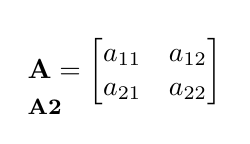
\begin{tikzpicture}[inner sep=0pt,outer sep=0pt]
\node[inner sep=0pt] (matA) {$\mathbf{A}=\begin{bmatrix}a_{11}&a_{12}\\a_{21}&a_{22}\end{bmatrix}$};
\useasboundingbox (-0.5\cellwd,-15.94pt) rectangle (0.5\cellwd,15.94pt);
\node[overlay,anchor=south west,font=\bfseries\footnotesize,xshift=\labxshiftB,yshift=0.36pt] at (current bounding box.south west) {A2};
\end{tikzpicture}
\end{minipage}
&
\begin{minipage}[c]{\cellwd}
\centering
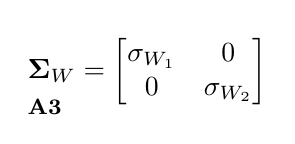
\begin{tikzpicture}[inner sep=0pt,outer sep=0pt]
\node[inner sep=0pt] (matSW) {$\mathbf{\Sigma}_W=\begin{bmatrix}\sigma_{W_1}&0\\0&\sigma_{W_2}\end{bmatrix}$};
\useasboundingbox (-0.5\cellwd,-15.94pt) rectangle (0.5\cellwd,15.94pt);
\node[overlay,anchor=south west,font=\bfseries\footnotesize,xshift=\labxshiftB,yshift=0.36pt] at (current bounding box.south west) {A3};
\end{tikzpicture}
\end{minipage}
\end{tabular}
% --- divider between the structure strip and row A ---
\vspace{6pt}
\hrule height 0.6pt
\vspace{6pt}
\nointerlineskip
% Row B: 2x3 grid of exported panel PDFs (see plot_topo_2node_dyad_subplot.m).
\renewcommand{\thesubfigure}{B1}
\phantomsubcaption\label{fig:dyad_B1}
\renewcommand{\thesubfigure}{B2}
\phantomsubcaption\label{fig:dyad_B2}
\renewcommand{\thesubfigure}{B3}
\phantomsubcaption\label{fig:dyad_B3}
\begin{tabular}{c@{\hspace{6pt}}|@{\hspace{6pt}}c@{\hspace{6pt}}|@{\hspace{6pt}}c}
\begin{minipage}[b]{\cellwd}
\centering
\begin{tikzpicture}[inner sep=0pt,outer sep=0pt]
\node[inner sep=0pt] (imgA1) {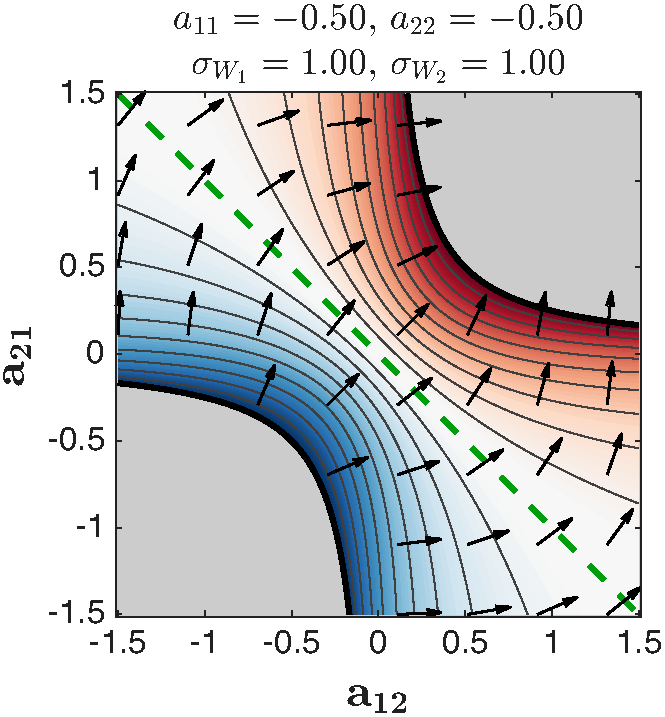
\includegraphics[width=\linewidth]{figures/topo_2node_dyad_figures/B1.pdf}};
\node[overlay,anchor=south west,font=\bfseries\footnotesize,xshift=-3.26pt,yshift=-2.42pt] at (imgA1.south west) {B1};
\end{tikzpicture}
\end{minipage}
&
\begin{minipage}[b]{\cellwd}
\centering
\begin{tikzpicture}[inner sep=0pt,outer sep=0pt]
\node[inner sep=0pt] (imgA2) {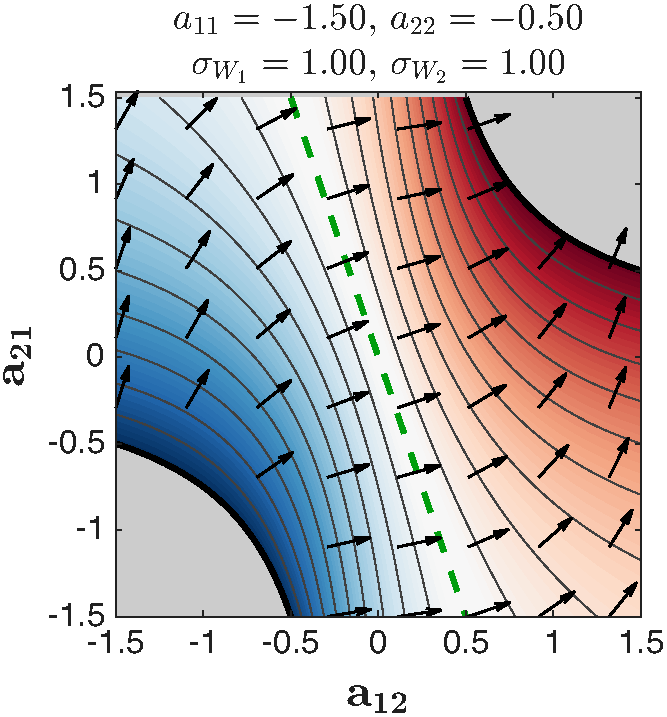
\includegraphics[width=\linewidth]{figures/topo_2node_dyad_figures/B2.pdf}};
\node[overlay,anchor=south west,font=\bfseries\footnotesize,xshift=\labxshiftB,yshift=-2.42pt] at (imgA2.south west) {B2};
\end{tikzpicture}
\end{minipage}
&
\begin{minipage}[b]{\cellwd}
\centering
\begin{tikzpicture}[inner sep=0pt,outer sep=0pt]
\node[inner sep=0pt] (imgA3) {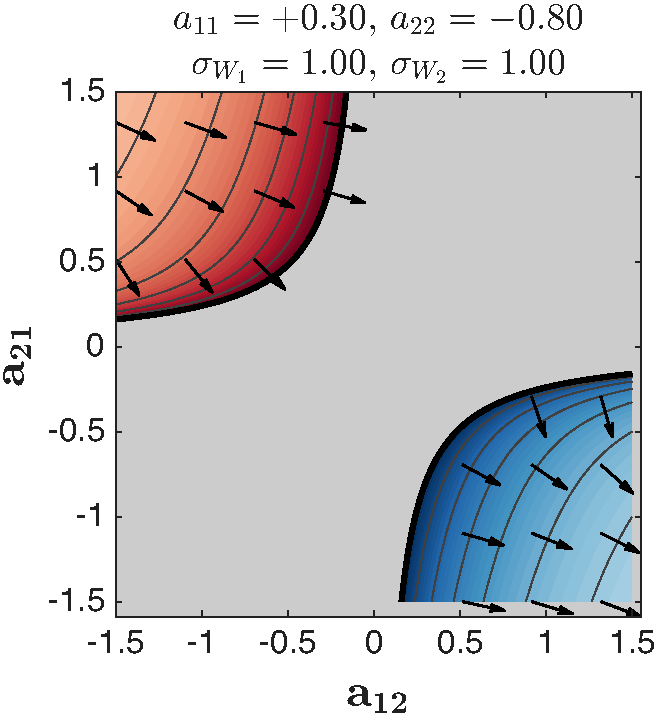
\includegraphics[width=\linewidth]{figures/topo_2node_dyad_figures/B3.pdf}};
\node[overlay,anchor=south west,font=\bfseries\footnotesize,xshift=\labxshiftB,yshift=-2.42pt] at (imgA3.south west) {B3};
\end{tikzpicture}
\end{minipage}
\end{tabular}
\par
% --- divider between row A and row B ---
\vspace{6pt}
\hrule height 0.6pt
\vspace{6pt}
\nointerlineskip
\renewcommand{\thesubfigure}{C1}
\phantomsubcaption\label{fig:dyad_C1}
\renewcommand{\thesubfigure}{C2}
\phantomsubcaption\label{fig:dyad_C2}
\renewcommand{\thesubfigure}{C3}
\phantomsubcaption\label{fig:dyad_C3}
\begin{tabular}{c@{\hspace{6pt}}|@{\hspace{6pt}}c@{\hspace{6pt}}|@{\hspace{6pt}}c}
\begin{minipage}[b]{\cellwd}
\centering
\begin{tikzpicture}[inner sep=0pt,outer sep=0pt]
\node[inner sep=0pt] (imgB1) {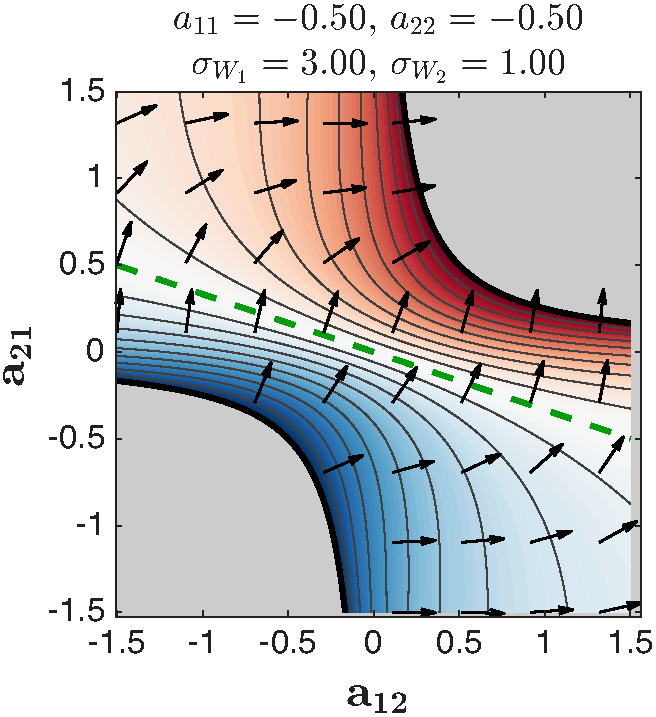
\includegraphics[width=\linewidth]{figures/topo_2node_dyad_figures/C1.pdf}};
\node[overlay,anchor=south west,font=\bfseries\footnotesize,xshift=-3.26pt,yshift=-2.42pt] at (imgB1.south west) {C1};
\end{tikzpicture}
\end{minipage}
&
\begin{minipage}[b]{\cellwd}
\centering
\begin{tikzpicture}[inner sep=0pt,outer sep=0pt]
\node[inner sep=0pt] (imgB2) {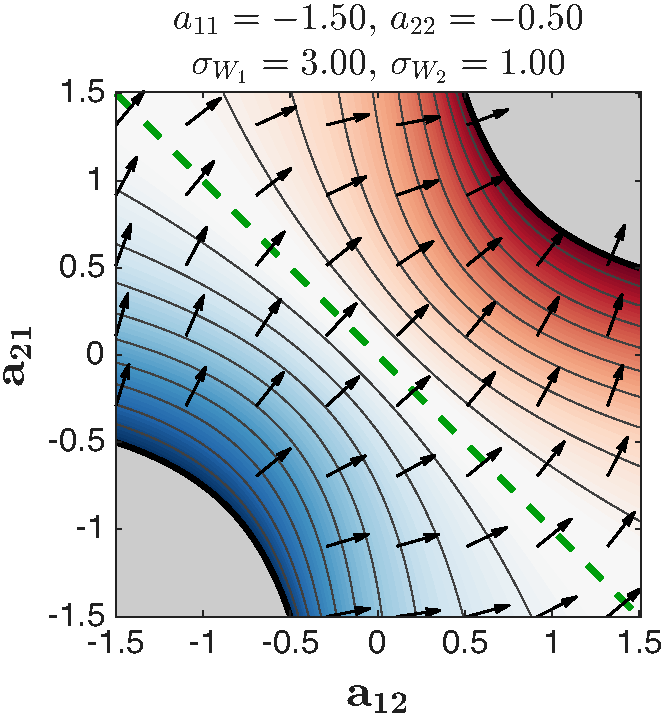
\includegraphics[width=\linewidth]{figures/topo_2node_dyad_figures/C2.pdf}};
\node[overlay,anchor=south west,font=\bfseries\footnotesize,xshift=\labxshiftB,yshift=-2.42pt] at (imgB2.south west) {C2};
\end{tikzpicture}
\end{minipage}
&
\begin{minipage}[b]{\cellwd}
\centering
\begin{tikzpicture}[inner sep=0pt,outer sep=0pt]
\node[inner sep=0pt] (imgB3) {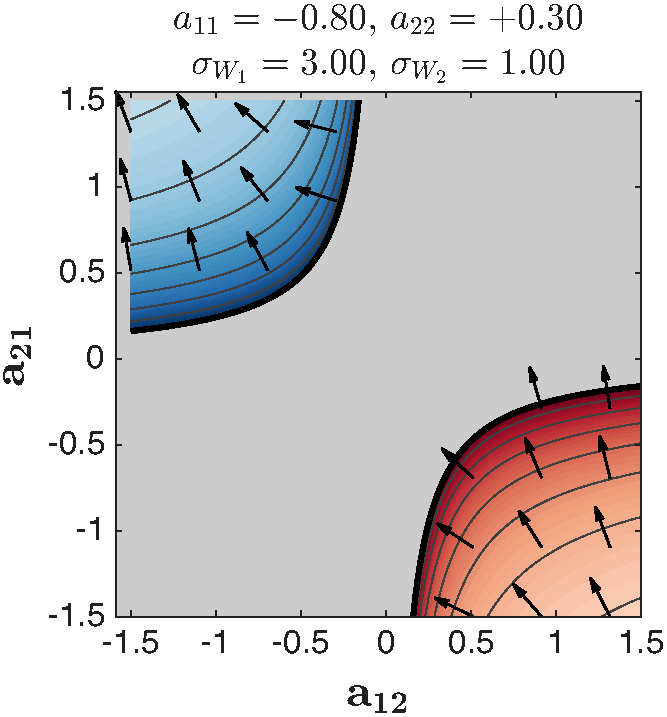
\includegraphics[width=\linewidth]{figures/topo_2node_dyad_figures/C3.pdf}};
\node[overlay,anchor=south west,font=\bfseries\footnotesize,xshift=\labxshiftB,yshift=-2.42pt] at (imgB3.south west) {C3};
\end{tikzpicture}
\end{minipage}
\end{tabular}
\par
% --- divider between row B and the colorbar ---
\vspace{6pt}
\hrule height 0.6pt
\vspace{6pt}
\nointerlineskip
% --- standalone colorbar, width \rowwd (see plot_topo_2node_dyad_subplot.m) ---
\includegraphics[width=\rowwd]{figures/topo_2node_dyad_figures/colorbar.pdf}
\par
\vspace{3pt}
\end{minipage}%
}}
\end{figure}

% \captionof (not \caption{}, so the caption can break across a page even
% though the figure itself can't) + counter rollback for the
% \phantomsubcaption bump above -- see the figure-template guide.
\addtocounter{figure}{-1}
\captionof{figure}{Dyadic network.
Each panel is a contour/vector field plot of equation~(\ref{eq:rho21_dyad})
over $a_{12},a_{21}\in[-1.5,1.5]$, for the self-connections
$a_{11}$, $a_{22}$ and noise variances $\sigma_{W_1}$, $\sigma_{W_2}$
indicated in its title.
Each column pairs two noise settings ($\sigma_{W_1}=1$ top,
$\sigma_{W_1}=3$ bottom) for the same self-connections; the third
column instead contrasts a dyad with its two self-connection
roles swapped.
Color encodes $\rho_{21}$ on a diverging scale from $-1$ (blue)
through white to $+1$ (red), with $|\rho_{21}|<0.05$ shown in white.
The dashed green curve marks $\rho_{21}=0$; the solid black curve
is the Hurwitz stability boundary, with the grey region outside it
(no steady state, $\rho_{21}$ undefined).}
\label{fig:rho21_dyad}

% ============================================================
\subsection*{Confounder}
% ============================================================

In the confounder network
(Figure~\ref{fig:rho21_confounder}\hyperref[fig:confounder_A1]{.A1}), nodes~1 and~2 have no direct causal connection, yet both are
driven by another node (node~3), which alone induces a (spurious)
correlation between them.
Here $a_{13}$ and $a_{23}$ are the causal influences of
node~3 on nodes~1 and~2, respectively. Because matrix $\mathbf{A}$ is upper triangular for this topology,
Hurwitz stability reduces to $a_{11}<0$, $a_{22}<0$, and
$a_{33}<0$.
Solving the Lyapunov equation for this confounder network
under the equal-diagonal simplification
$a_{11}=a_{22}=a_{33}=a$ yields (see
% Headline result: confounder rho_21, derived in Appendix D.
\hyperref[app:appD]{Appendix~D},
equation~\ref{eq:d26_rho21_confounder}),
\begin{equation}
\rho_{21} = \frac{
  a_{13}\,a_{23}\,\sigma_{W_3}
}{
  \sqrt{
    \bigl(2a^2\sigma_{W_1}+a_{13}^2\sigma_{W_3}\bigr)
    \bigl(2a^2\sigma_{W_2}+a_{23}^2\sigma_{W_3}\bigr)
  }
}.
\label{eq:rho21_confounder}
\end{equation}

% ============================================================
% Confounder figure -- individual-panel template (produced per
% tasks/stage3_tasks_plot_networks/stage3_topo_x-node_figure_template_instructions.md).
% Panels exported by scripts/plot_networks/plot_topo_3node_confounder_subplot.m
% to figures/topo_3node_confounder_figures/. Two subplot rows (A/B); no row C.
% ============================================================
\begin{figure}[H]
\centering
{\setlength{\fboxrule}{0.6pt}\setlength{\arrayrulewidth}{0.6pt}%
\fbox{%
\begin{minipage}{\dimexpr\textwidth-2\fboxsep-2\fboxrule\relax}
\centering
\setlength{\cellwd}{\dimexpr(0.95\linewidth-12pt)/3\relax}
\setlength{\rowwd}{\dimexpr3\cellwd+12pt\relax}
\setlength{\labxshiftB}{-0.26pt}
\vspace{3pt}
% --- title ---
{\normalsize\textbf{$\rho_{21}$ as a function of $a_{13}$ and $a_{23}$ (confounder)}}\par

\vspace{6pt}\hrule height 0.6pt\vspace{6pt}\nointerlineskip   

% Divider 4
% --- structure strip: diagram | A | Sigma_W ---
% --- structure strip labels A1-A3 -- see dyad figure's comment
% for the label mechanism.
\renewcommand{\thesubfigure}{A1}
\phantomsubcaption\label{fig:confounder_A1}
\renewcommand{\thesubfigure}{A2}
\phantomsubcaption\label{fig:confounder_A2}
\renewcommand{\thesubfigure}{A3}
\phantomsubcaption\label{fig:confounder_A3}
\begin{tabular}{c@{\hspace{6pt}}|@{\hspace{6pt}}c@{\hspace{6pt}}|@{\hspace{6pt}}c}
\begin{minipage}[c]{\cellwd}
\centering
\def\a{1.0 cm}
\def\nodeSize{0.7}
\def\r{0.5*\nodeSize cm}
\begin{tikzpicture}[inner sep=0pt,outer sep=0pt]
\node[inner sep=0pt] (confounderDiagram) {%
\begin{tikzpicture}[
    >={Stealth[length=3mm,width=2mm]},
    every node/.style={circle,draw,
        minimum size=\nodeSize cm}]
\node (1) at (-\a,0)          {1};
\node (2) at (\a,0)           {2};
\node (3) at (0,{sqrt(3)*\a}) {3};
\draw[->] (3) to[bend right=12] (1);
\draw[->] (3) to[bend left=12]  (2);
\selfloop{1}{1}
\selfloop{2}{2}
\selfloop{3}{3}
\end{tikzpicture}%
};
\useasboundingbox (-0.5\cellwd,-45.35pt) rectangle (0.5\cellwd,45.35pt);
\node[overlay,anchor=south west,font=\bfseries\footnotesize,xshift=-3.26pt,yshift=3.91pt] at (current bounding box.south west) {A1};
\end{tikzpicture}
\end{minipage}
&
\begin{minipage}[c]{\cellwd}
\centering
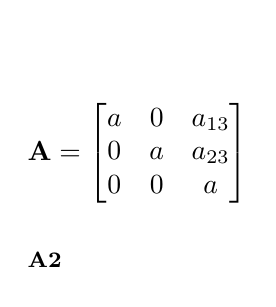
\begin{tikzpicture}[inner sep=0pt,outer sep=0pt]
\node[inner sep=0pt] (matA) {$\mathbf{A}=\begin{bmatrix}
a & 0 & a_{13}\\
0 & a & a_{23}\\
0 & 0 & a
\end{bmatrix}$};
\useasboundingbox (-0.5\cellwd,-45.35pt) rectangle (0.5\cellwd,45.35pt);
\node[overlay,anchor=south west,font=\bfseries\footnotesize,xshift=\labxshiftB,yshift=3.91pt] at (current bounding box.south west) {A2};
\end{tikzpicture}
\end{minipage}
&
\begin{minipage}[c]{\cellwd}
\centering
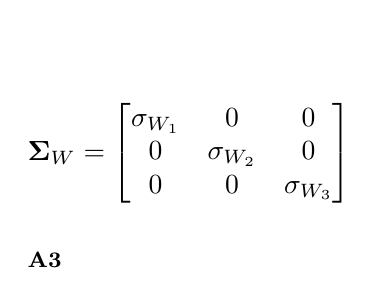
\begin{tikzpicture}[inner sep=0pt,outer sep=0pt]
\node[inner sep=0pt] (matSW) {$\mathbf{\Sigma}_W=\begin{bmatrix}
\sigma_{W_1}&0&0\\0&\sigma_{W_2}&0\\0&0&\sigma_{W_3}
\end{bmatrix}$};
\useasboundingbox (-0.5\cellwd,-45.35pt) rectangle (0.5\cellwd,45.35pt);
\node[overlay,anchor=south west,font=\bfseries\footnotesize,xshift=\labxshiftB,yshift=3.91pt] at (current bounding box.south west) {A3};
\end{tikzpicture}
\end{minipage}
\end{tabular}

\vspace{6pt}\hrule height 0.6pt\vspace{6pt}\nointerlineskip   % 


%Divider 1
% --- Row A ---
\renewcommand{\thesubfigure}{B1}\phantomsubcaption\label{fig:confounder_B1}
\renewcommand{\thesubfigure}{B2}\phantomsubcaption\label{fig:confounder_B2}
\renewcommand{\thesubfigure}{B3}\phantomsubcaption\label{fig:confounder_B3}
\begin{tabular}{c@{\hspace{6pt}}|@{\hspace{6pt}}c@{\hspace{6pt}}|@{\hspace{6pt}}c}
\begin{minipage}[b]{\cellwd}
\centering
\begin{tikzpicture}[inner sep=0pt,outer sep=0pt]
\node[inner sep=0pt] (imgA1) {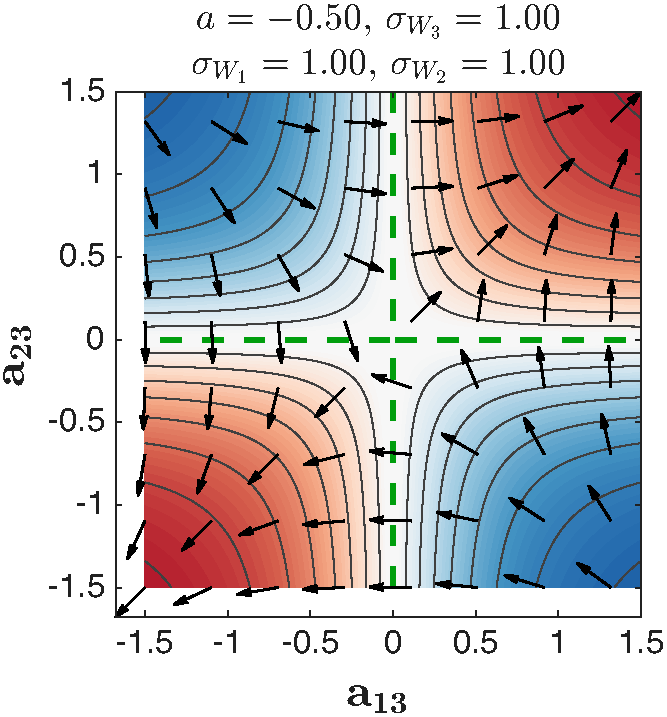
\includegraphics[width=\linewidth]{figures/topo_3node_confounder_figures/B1.pdf}};
\node[overlay,anchor=south west,font=\bfseries\footnotesize,xshift=-3.26pt,yshift=0.58pt] at (imgA1.south west) {B1};
\end{tikzpicture}
\end{minipage}
&
\begin{minipage}[b]{\cellwd}
\centering
\begin{tikzpicture}[inner sep=0pt,outer sep=0pt]
\node[inner sep=0pt] (imgA2) {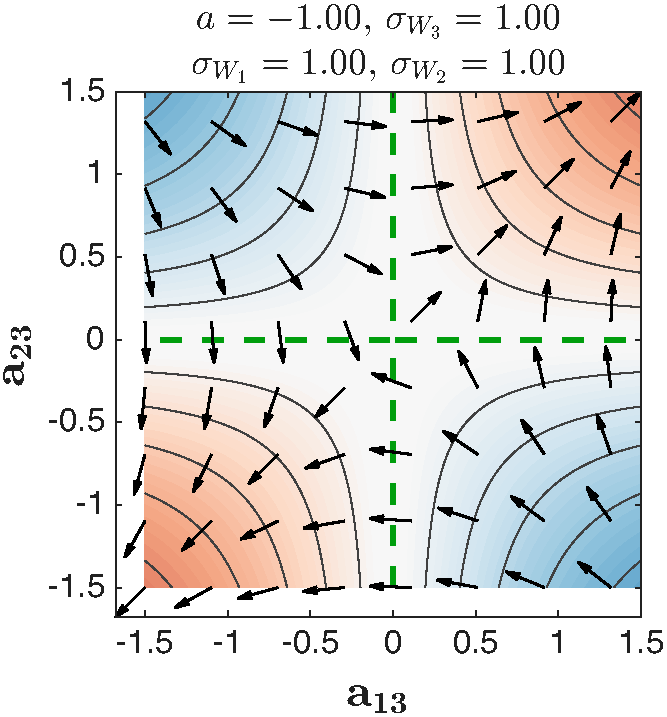
\includegraphics[width=\linewidth]{figures/topo_3node_confounder_figures/B2.pdf}};
\node[overlay,anchor=south west,font=\bfseries\footnotesize,xshift=\labxshiftB,yshift=0.58pt] at (imgA2.south west) {B2};
\end{tikzpicture}
\end{minipage}
&
\begin{minipage}[b]{\cellwd}
\centering
\begin{tikzpicture}[inner sep=0pt,outer sep=0pt]
\node[inner sep=0pt] (imgA3) {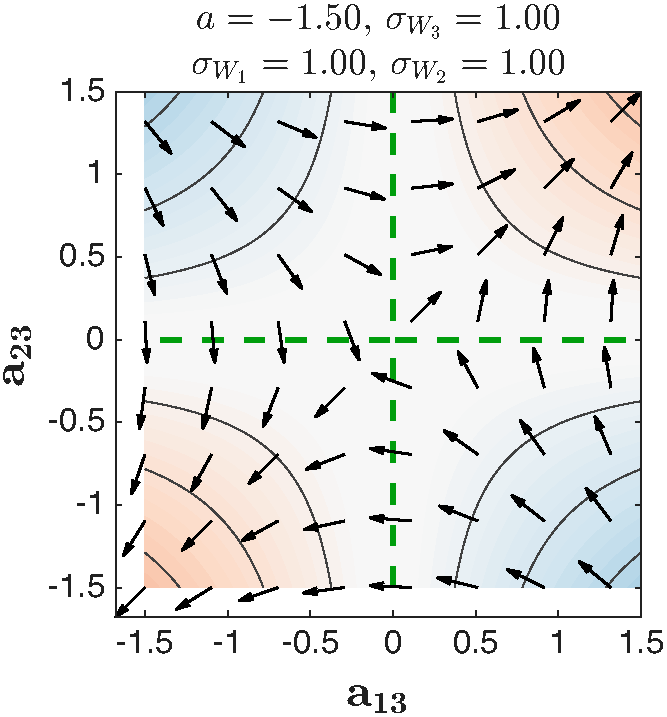
\includegraphics[width=\linewidth]{figures/topo_3node_confounder_figures/B3.pdf}};
\node[overlay,anchor=south west,font=\bfseries\footnotesize,xshift=\labxshiftB,yshift=0.58pt] at (imgA3.south west) {B3};
\end{tikzpicture}
\end{minipage}
\end{tabular}
\par
\vspace{6pt}\hrule height 0.6pt\vspace{6pt}\nointerlineskip   

% Divider 2
% --- Row B ---
\renewcommand{\thesubfigure}{C1}\phantomsubcaption\label{fig:confounder_C1}
\renewcommand{\thesubfigure}{C2}\phantomsubcaption\label{fig:confounder_C2}
\renewcommand{\thesubfigure}{C3}\phantomsubcaption\label{fig:confounder_C3}
\begin{tabular}{c@{\hspace{6pt}}|@{\hspace{6pt}}c@{\hspace{6pt}}|@{\hspace{6pt}}c}
\begin{minipage}[b]{\cellwd}
\centering
\begin{tikzpicture}[inner sep=0pt,outer sep=0pt]
\node[inner sep=0pt] (imgB1) {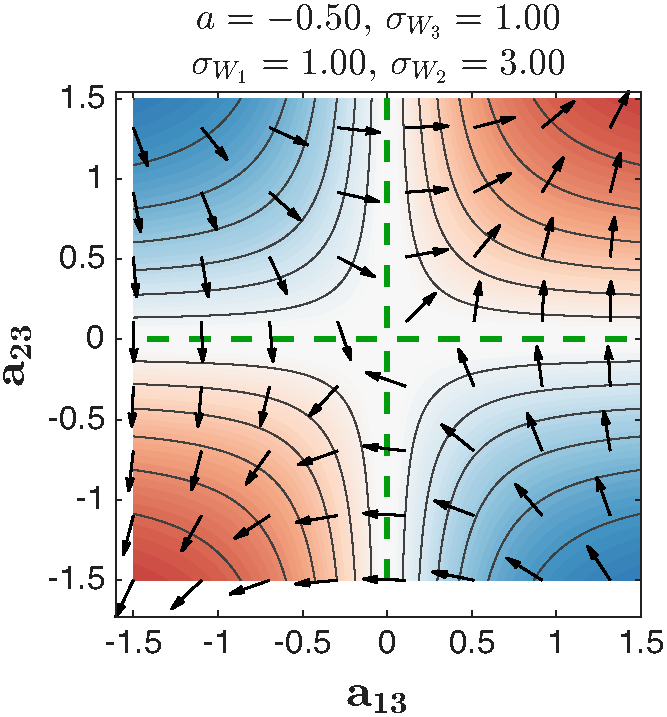
\includegraphics[width=\linewidth]{figures/topo_3node_confounder_figures/C1.pdf}};
\node[overlay,anchor=south west,font=\bfseries\footnotesize,xshift=-3.26pt,yshift=0.58pt] at (imgB1.south west) {C1};
\end{tikzpicture}
\end{minipage}
&
\begin{minipage}[b]{\cellwd}
\centering
\begin{tikzpicture}[inner sep=0pt,outer sep=0pt]
\node[inner sep=0pt] (imgB2) {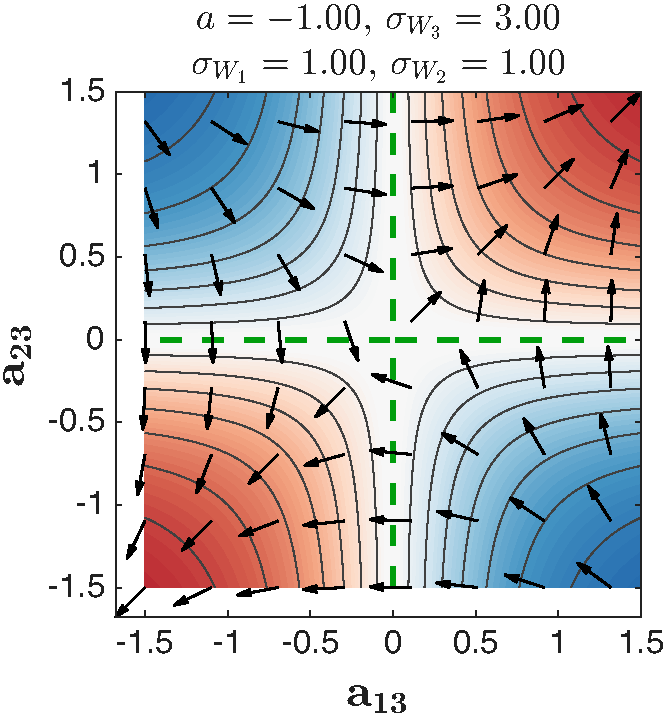
\includegraphics[width=\linewidth]{figures/topo_3node_confounder_figures/C2.pdf}};
\node[overlay,anchor=south west,font=\bfseries\footnotesize,xshift=\labxshiftB,yshift=0.58pt] at (imgB2.south west) {C2};
\end{tikzpicture}
\end{minipage}
&
\begin{minipage}[b]{\cellwd}
\centering
\begin{tikzpicture}[inner sep=0pt,outer sep=0pt]
\node[inner sep=0pt] (imgB3) {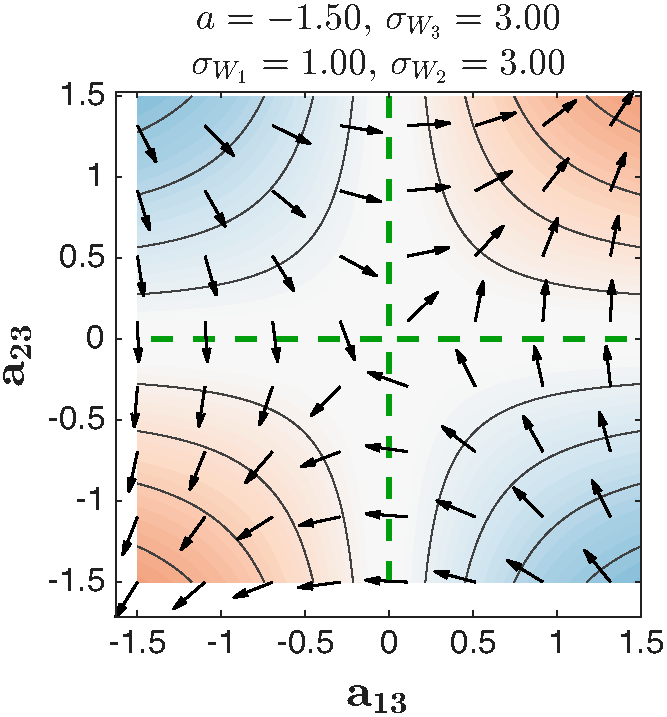
\includegraphics[width=\linewidth]{figures/topo_3node_confounder_figures/C3.pdf}};
\node[overlay,anchor=south west,font=\bfseries\footnotesize,xshift=\labxshiftB,yshift=0.58pt] at (imgB3.south west) {C3};
\end{tikzpicture}
\end{minipage}
\end{tabular}

\vspace{6pt}\hrule height 0.6pt\vspace{6pt}\nointerlineskip   

% Divider 3
% --- colorbar (spans \rowwd) ---
\includegraphics[width=\rowwd]{figures/topo_3node_confounder_figures/colorbar.pdf}
\par
\vspace{3pt}
\end{minipage}%
}}
\end{figure}

% caption OUTSIDE the float; \addtocounter rolls back the phantomsubcaption bump
\addtocounter{figure}{-1}
\captionof{figure}{Confounder network.
Each panel is a contour/vector field plot of equation~(\ref{eq:rho21_confounder}) for
$\rho_{21}$ over $a_{13},a_{23}\in[-1.5,1.5]$, for the combination of the
common self-connection $a$, $\sigma_{W_2}$, and $\sigma_{W_3}$ shown in
each panel's title ($\sigma_{W_1}=1$ throughout); across the three
columns the common self-inhibition strengthens ($a=-0.5,-1.0,-1.5$).
Color encodes $\rho_{21}$ on a diverging scale from $-1$ (blue) through white
to $+1$ (red); values with $|\rho_{21}|<0.05$ are shown in white.
The dashed green lines mark $\rho_{21}=0$ exactly, forming a cross along
$a_{13}=0$ and $a_{23}=0$.}
\label{fig:rho21_confounder}

\vspace{6pt}
From equation~(\ref{eq:rho21_confounder}), we see that the numerator $a_{13}\,a_{23}\,\sigma_{W_3}$ is zero if either $a_{13}=0$ or $a_{23}=0$. Therefore, the
correlation vanishes exactly whenever either connection from
node~3 is absent (the green zero-contour cross in
Figure~\ref{fig:rho21_confounder}), showing that the spurious correlation between node~1 and node~2 is
entirely driven by the common input, node~3. Correspondingly, the
sign of $\rho_{21}$ equals the sign of $a_{13}\,a_{23}$,
positive if node~3 drives both nodes in the same direction
and negative if in opposite directions.
As the self-inhibition strength $|a|$ increases relative to
the driving connections $a_{13}$ and $a_{23}$ (left to right
across the panels of Figure~\ref{fig:rho21_confounder}), the
magnitude of $\rho_{21}$ decreases.

% ============================================================
\subsection*{Collider}
% ============================================================

The collider network
(Figure~\ref{fig:rho31_collider}\hyperref[fig:collider_A1]{.A1})
is termed a collider because causal paths from two
independent sources ``collide'' at node~3 \citep{Pearl2009}.
Both node~1 and node~2 send unidirectional connections to node~3, with no direct connection
between nodes~1 and~2. Because
$\mathbf{A}$
(Figure~\ref{fig:rho31_collider}\hyperref[fig:collider_A2]{.A2})
is lower triangular for this topology,
Hurwitz stability reduces to $a<0$ under the equal-diagonal
simplification $a_{11}=a_{22}=a_{33}=a$.
% Headline result: collider rho_21 vanishes identically (derived in
% Appendix D) -- the notable negative case; rho_31/rho_32 below are the
% topology-specific quantities that are actually informative here.
Solving the Lyapunov equation for this collider network gives us, $\sigma_{21}=0$ (see
\hyperref[app:appD]{Appendix~D}). Therefore,
\begin{equation}
\rho_{21} = 0.
\label{eq:rho21_collider}
\end{equation}
The correlations $\rho_{31}$ and $\rho_{32}$ are in general
nonzero, however, since each of nodes~1 and~2 drives node~3
directly (see \hyperref[app:appD]{Appendix~D}),
\begin{equation}
\rho_{31} = \frac{a_{31}\,\sigma_{W_1}}
{\sqrt{2\sigma_{W_1}
  \bigl(2a^2\sigma_{W_3}+a_{32}^2\sigma_{W_2}
        +a_{31}^2\sigma_{W_1}\bigr)}}.
\label{eq:rho31_collider_main}
\end{equation}
\begin{equation}
\rho_{32} = \frac{a_{32}\,\sigma_{W_2}}
{\sqrt{2\sigma_{W_2}
  \bigl(2a^2\sigma_{W_3}+a_{32}^2\sigma_{W_2}
        +a_{31}^2\sigma_{W_1}\bigr)}}.
\label{eq:rho32_collider_main}
\end{equation}
Notice the symmetry in equations (\ref{eq:rho31_collider_main}) \& (\ref{eq:rho32_collider_main}) and that $\rho_{31}$ carries the sign of $a_{31}$ and
depends on the strengths of \emph{both} causal connections
($a_{31}$ and $a_{32}$), through their influences on
the variance of node~3 in the denominator of equation (\ref{eq:rho31_collider_main}).
Thus, strengthening the causal influence from node~2 to
node~3 weakens the correlation between node~1 and node~3,
even though node~1 and node~2 remain uncoupled and
uncorrelated.
As Figure~\ref{fig:rho31_collider}\hyperref[fig:collider_B1]{.B1}
shows, $\rho_{31}$ (and
correspondingly $\rho_{32}$) can be strong for suitable
parameter values of $a_{31}$ and $a_{32}$, yet $\rho_{21}$ remains $0$ regardless.
This shows that correlation is not \emph{transitive}, a point
we discuss in more depth in the Discussion section.

% ============================================================
% Collider figure -- individual-panel template (produced per
% tasks/stage3_tasks_plot_networks/stage3_topo_x-node_figure_template_instructions.md).
% Panels exported by scripts/plot_networks/plot_topo_3node_collider_subplot.m
% to figures/topo_3node_collider_figures/. Two subplot rows (A/B); no row C.
% ============================================================
\begin{figure}[H]
\centering
{\setlength{\fboxrule}{0.6pt}\setlength{\arrayrulewidth}{0.6pt}%
\fbox{%
\begin{minipage}{\dimexpr\textwidth-2\fboxsep-2\fboxrule\relax}
\centering
\setlength{\cellwd}{\dimexpr(0.95\linewidth-12pt)/3\relax}
\setlength{\rowwd}{\dimexpr3\cellwd+12pt\relax}
\setlength{\labxshiftB}{-0.26pt}
\vspace{3pt}
% --- title ---
{\normalsize\textbf{$\rho_{31}$ as a function of $a_{31}$ and $a_{32}$ (collider)}}\par
\vspace{6pt}\hrule height 0.6pt\vspace{6pt}\nointerlineskip   % Divider 4
% --- structure strip: diagram | A | Sigma_W ---
% --- structure strip labels A1-A3 -- see dyad figure's comment
% for the label mechanism.
\renewcommand{\thesubfigure}{A1}
\phantomsubcaption\label{fig:collider_A1}
\renewcommand{\thesubfigure}{A2}
\phantomsubcaption\label{fig:collider_A2}
\renewcommand{\thesubfigure}{A3}
\phantomsubcaption\label{fig:collider_A3}
\begin{tabular}{c@{\hspace{6pt}}|@{\hspace{6pt}}c@{\hspace{6pt}}|@{\hspace{6pt}}c}
\begin{minipage}[c]{\cellwd}
\centering
\def\a{1.0 cm}
\def\nodeSize{0.7}
\def\r{0.5*\nodeSize cm}
\begin{tikzpicture}[inner sep=0pt,outer sep=0pt]
\node[inner sep=0pt] (colliderDiagram) {%
\begin{tikzpicture}[
    >={Stealth[length=3mm,width=2mm]},
    every node/.style={circle,draw,
        minimum size=\nodeSize cm}]
\node (1) at (-\a,0)          {1};
\node (2) at (\a,0)           {2};
\node (3) at (0,{sqrt(3)*\a}) {3};
\draw[->] (1) to[bend left=12]  (3);
\draw[->] (2) to[bend right=12] (3);
\selfloop{1}{1}
\selfloop{2}{2}
\selfloop{3}{3}
\end{tikzpicture}%
};
\useasboundingbox (-0.5\cellwd,-45.35pt) rectangle (0.5\cellwd,45.35pt);
\node[overlay,anchor=south west,font=\bfseries\footnotesize,xshift=-3.26pt,yshift=3.91pt] at (current bounding box.south west) {A1};
\end{tikzpicture}
\end{minipage}
&
\begin{minipage}[c]{\cellwd}
\centering
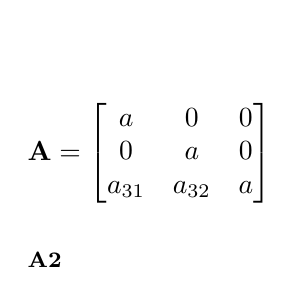
\begin{tikzpicture}[inner sep=0pt,outer sep=0pt]
\node[inner sep=0pt] (matA) {$\mathbf{A}=\begin{bmatrix}
a      & 0      & 0\\
0      & a      & 0\\
a_{31} & a_{32} & a
\end{bmatrix}$};
\useasboundingbox (-0.5\cellwd,-45.35pt) rectangle (0.5\cellwd,45.35pt);
\node[overlay,anchor=south west,font=\bfseries\footnotesize,xshift=\labxshiftB,yshift=3.91pt] at (current bounding box.south west) {A2};
\end{tikzpicture}
\end{minipage}
&
\begin{minipage}[c]{\cellwd}
\centering
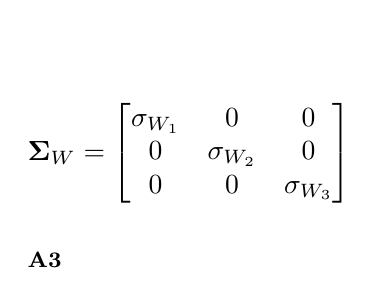
\begin{tikzpicture}[inner sep=0pt,outer sep=0pt]
\node[inner sep=0pt] (matSW) {$\mathbf{\Sigma}_W=\begin{bmatrix}
\sigma_{W_1}&0&0\\0&\sigma_{W_2}&0\\0&0&\sigma_{W_3}
\end{bmatrix}$};
\useasboundingbox (-0.5\cellwd,-45.35pt) rectangle (0.5\cellwd,45.35pt);
\node[overlay,anchor=south west,font=\bfseries\footnotesize,xshift=\labxshiftB,yshift=3.91pt] at (current bounding box.south west) {A3};
\end{tikzpicture}
\end{minipage}
\end{tabular}
\vspace{6pt}\hrule height 0.6pt\vspace{6pt}\nointerlineskip   % Divider 1
% --- Row A ---
\renewcommand{\thesubfigure}{B1}\phantomsubcaption\label{fig:collider_B1}
\renewcommand{\thesubfigure}{B2}\phantomsubcaption\label{fig:collider_B2}
\renewcommand{\thesubfigure}{B3}\phantomsubcaption\label{fig:collider_B3}
\begin{tabular}{c@{\hspace{6pt}}|@{\hspace{6pt}}c@{\hspace{6pt}}|@{\hspace{6pt}}c}
\begin{minipage}[b]{\cellwd}
\centering
\begin{tikzpicture}[inner sep=0pt,outer sep=0pt]
\node[inner sep=0pt] (imgA1) {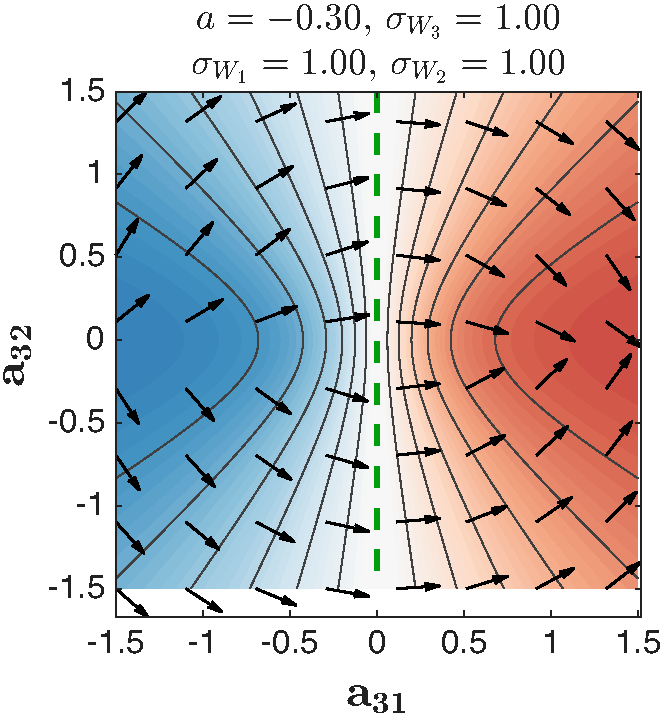
\includegraphics[width=\linewidth]{figures/topo_3node_collider_figures/B1.pdf}};
\node[overlay,anchor=south west,font=\bfseries\footnotesize,xshift=-3.26pt,yshift=0.58pt] at (imgA1.south west) {B1};
\end{tikzpicture}
\end{minipage}
&
\begin{minipage}[b]{\cellwd}
\centering
\begin{tikzpicture}[inner sep=0pt,outer sep=0pt]
\node[inner sep=0pt] (imgA2) {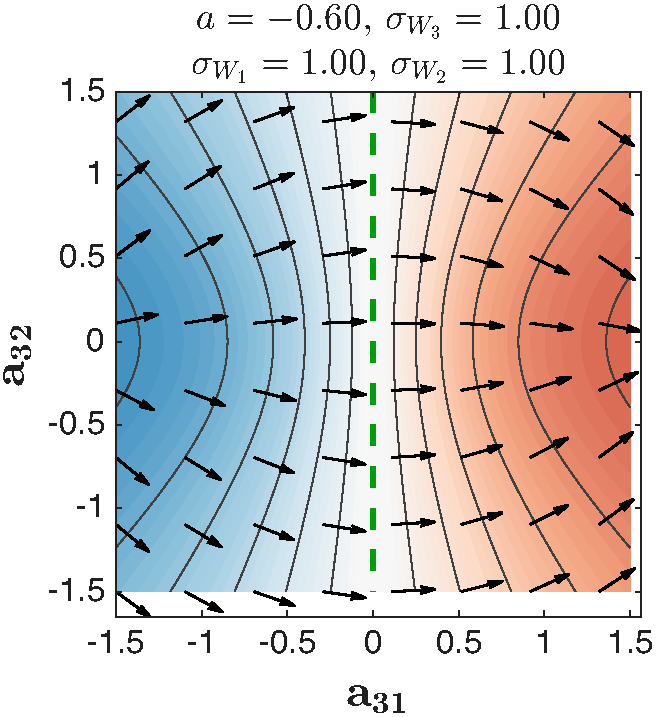
\includegraphics[width=\linewidth]{figures/topo_3node_collider_figures/B2.pdf}};
\node[overlay,anchor=south west,font=\bfseries\footnotesize,xshift=\labxshiftB,yshift=0.58pt] at (imgA2.south west) {B2};
\end{tikzpicture}
\end{minipage}
&
\begin{minipage}[b]{\cellwd}
\centering
\begin{tikzpicture}[inner sep=0pt,outer sep=0pt]
\node[inner sep=0pt] (imgA3) {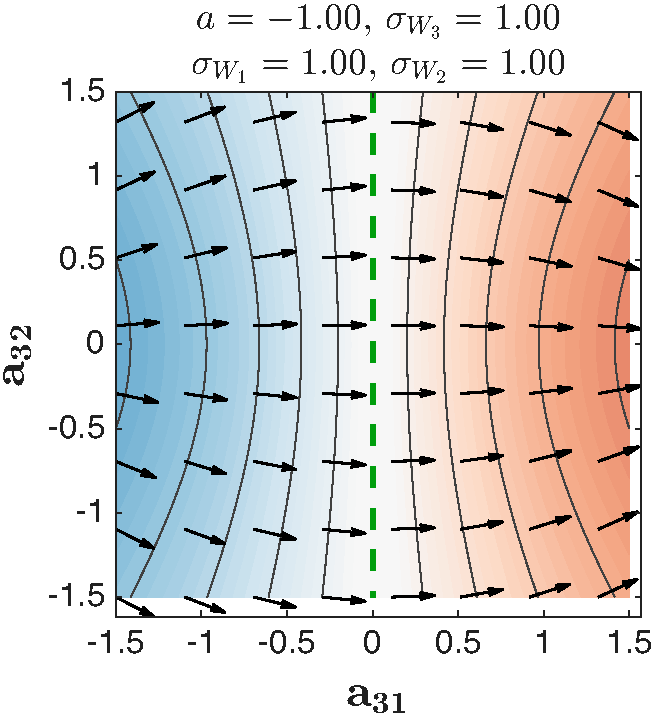
\includegraphics[width=\linewidth]{figures/topo_3node_collider_figures/B3.pdf}};
\node[overlay,anchor=south west,font=\bfseries\footnotesize,xshift=\labxshiftB,yshift=0.58pt] at (imgA3.south west) {B3};
\end{tikzpicture}
\end{minipage}
\end{tabular}
\par
\vspace{6pt}\hrule height 0.6pt\vspace{6pt}\nointerlineskip   % Divider 2
% --- Row B ---
\renewcommand{\thesubfigure}{C1}\phantomsubcaption\label{fig:collider_C1}
\renewcommand{\thesubfigure}{C2}\phantomsubcaption\label{fig:collider_C2}
\renewcommand{\thesubfigure}{C3}\phantomsubcaption\label{fig:collider_C3}
\begin{tabular}{c@{\hspace{6pt}}|@{\hspace{6pt}}c@{\hspace{6pt}}|@{\hspace{6pt}}c}
\begin{minipage}[b]{\cellwd}
\centering
\begin{tikzpicture}[inner sep=0pt,outer sep=0pt]
\node[inner sep=0pt] (imgB1) {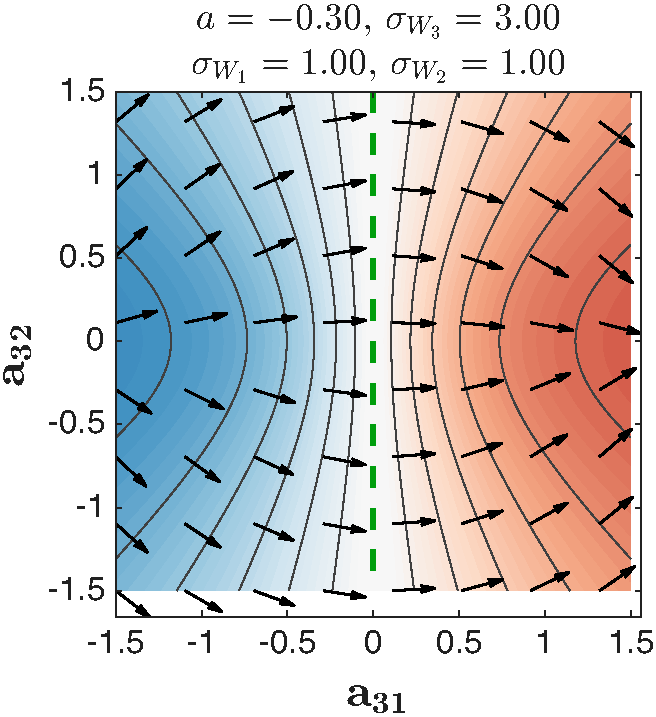
\includegraphics[width=\linewidth]{figures/topo_3node_collider_figures/C1.pdf}};
\node[overlay,anchor=south west,font=\bfseries\footnotesize,xshift=-3.26pt,yshift=0.58pt] at (imgB1.south west) {C1};
\end{tikzpicture}
\end{minipage}
&
\begin{minipage}[b]{\cellwd}
\centering
\begin{tikzpicture}[inner sep=0pt,outer sep=0pt]
\node[inner sep=0pt] (imgB2) {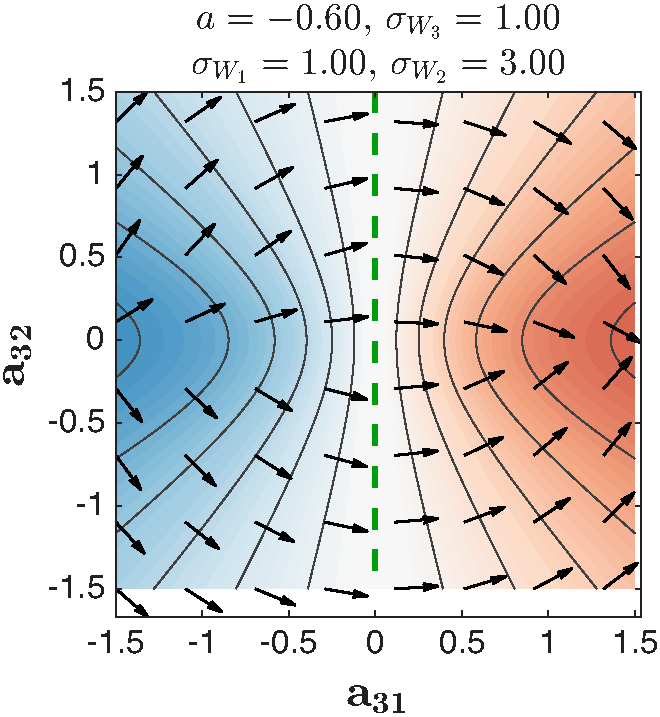
\includegraphics[width=\linewidth]{figures/topo_3node_collider_figures/C2.pdf}};
\node[overlay,anchor=south west,font=\bfseries\footnotesize,xshift=\labxshiftB,yshift=0.58pt] at (imgB2.south west) {C2};
\end{tikzpicture}
\end{minipage}
&
\begin{minipage}[b]{\cellwd}
\centering
\begin{tikzpicture}[inner sep=0pt,outer sep=0pt]
\node[inner sep=0pt] (imgB3) {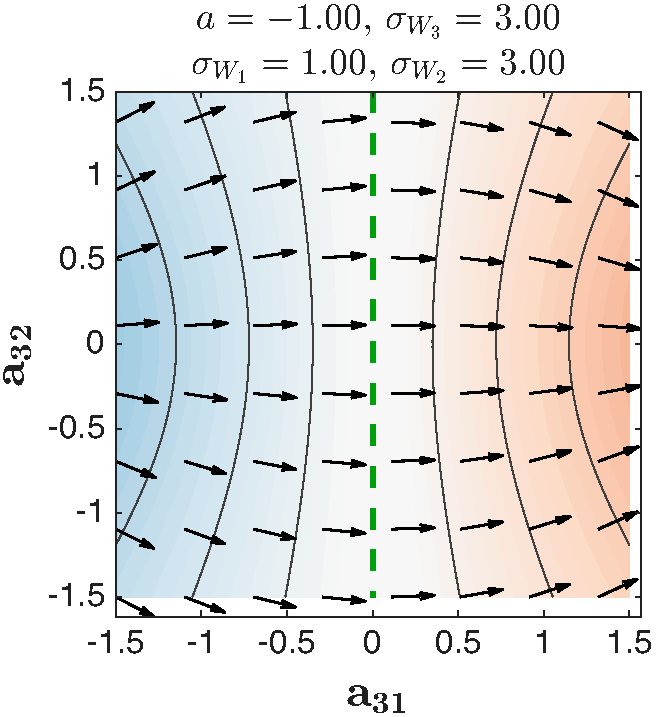
\includegraphics[width=\linewidth]{figures/topo_3node_collider_figures/C3.pdf}};
\node[overlay,anchor=south west,font=\bfseries\footnotesize,xshift=\labxshiftB,yshift=0.58pt] at (imgB3.south west) {C3};
\end{tikzpicture}
\end{minipage}
\end{tabular}

\vspace{6pt}\hrule height 0.6pt\vspace{6pt}\nointerlineskip   % Divider 3
% --- colorbar (spans \rowwd) ---
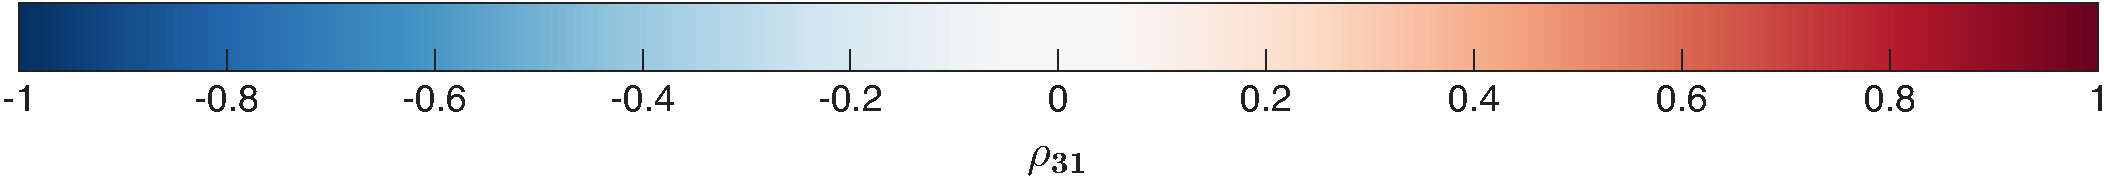
\includegraphics[width=\rowwd]{figures/topo_3node_collider_figures/colorbar.pdf}
\par
\vspace{3pt}
\end{minipage}%
}}
\end{figure}

% caption OUTSIDE the float; \addtocounter rolls back the phantomsubcaption bump
\addtocounter{figure}{-1}
\captionof{figure}{Collider network.
Each panel is a contour/vector field plot of equation~(\ref{eq:rho31_collider_main}) for
$\rho_{31}$ over $a_{31},a_{32}\in[-1.5,1.5]$, for the combination of the
common self-connection $a$, $\sigma_{W_2}$, and $\sigma_{W_3}$ shown in
each panel's title ($\sigma_{W_1}=1$ throughout); $a$ strengthens across
the three columns ($a=-0.3,-0.6,-1.0$).
Color encodes $\rho_{31}$ on a diverging scale from $-1$ (blue) through white
to $+1$ (red); values with $|\rho_{31}|<0.05$ are shown in white.
The dashed green line marks $\rho_{31}=0$ exactly, at $a_{31}=0$.}
\label{fig:rho31_collider}

% ============================================================
\subsection*{One-Way Mediator}
% ============================================================

The mediator network
(Figure~\ref{fig:rho21_mediator}\hyperref[fig:mediator_A1]{.A1})
is one in which node~1 influences node~2 not directly but
through an intermediary node~3.
Therefore, any observed correlation between node~1 and
node~2 must be mediated by node~3.
Hurwitz stability requires that $a<0$ under the equal-diagonal
simplification $a_{11}=a_{22}=a_{33}=a$.
Solving the Lyapunov equation for this mediator network yields
% Headline result: one-way mediator rho_21, derived in Appendix D.
(\hyperref[app:appD]{Appendix~D},
equation~\ref{eq:rho21_mediator}),
\begin{equation}
\rho_{21} = \frac{
  a_{31}\,a_{23}\,\sigma_{W_1}
}{
  \sqrt{2\sigma_{W_1}
        \bigl(8a^4\sigma_{W_2}
              +4a^2 a_{23}^2\sigma_{W_3}
              +3a_{23}^2 a_{31}^2\sigma_{W_1}\bigr)}
}.
\label{eq:rho21_mediator_main}
\end{equation}

% ============================================================
% Mediator figure -- individual-panel template (produced per
% tasks/stage3_tasks_plot_networks/stage3_topo_x-node_figure_template_instructions.md).
% Panels exported by scripts/plot_networks/plot_topo_3node_mediator_subplot.m
% to figures/topo_3node_mediator_figures/. Two subplot rows (A/B); no row C.
% ============================================================
\begin{figure}[H]
\centering
{\setlength{\fboxrule}{0.6pt}\setlength{\arrayrulewidth}{0.6pt}%
\fbox{%
\begin{minipage}{\dimexpr\textwidth-2\fboxsep-2\fboxrule\relax}
\centering
\setlength{\cellwd}{\dimexpr(0.95\linewidth-12pt)/3\relax}
\setlength{\rowwd}{\dimexpr3\cellwd+12pt\relax}
\setlength{\labxshiftB}{-0.26pt}
\vspace{3pt}
% --- title ---
{\normalsize\textbf{$\rho_{21}$ as a function of $a_{31}$ and $a_{23}$ (mediator)}}\par
\vspace{6pt}\hrule height 0.6pt\vspace{6pt}\nointerlineskip   % Divider 4
% --- structure strip: diagram | A | Sigma_W ---
% --- structure strip labels A1-A3 -- see dyad figure's comment
% for the label mechanism.
\renewcommand{\thesubfigure}{A1}
\phantomsubcaption\label{fig:mediator_A1}
\renewcommand{\thesubfigure}{A2}
\phantomsubcaption\label{fig:mediator_A2}
\renewcommand{\thesubfigure}{A3}
\phantomsubcaption\label{fig:mediator_A3}
\begin{tabular}{c@{\hspace{6pt}}|@{\hspace{6pt}}c@{\hspace{6pt}}|@{\hspace{6pt}}c}
\begin{minipage}[c]{\cellwd}
\centering
\def\a{1.0 cm}
\def\nodeSize{0.7}
\def\r{0.5*\nodeSize cm}
\begin{tikzpicture}[inner sep=0pt,outer sep=0pt]
\node[inner sep=0pt] (mediatorDiagram) {%
\begin{tikzpicture}[
    >={Stealth[length=3mm,width=2mm]},
    every node/.style={circle,draw,
        minimum size=\nodeSize cm}]
\node (1) at (-\a,0)          {1};
\node (2) at (\a,0)           {2};
\node (3) at (0,{sqrt(3)*\a}) {3};
\draw[->] (1) to[bend left=12]  (3);
\draw[->] (3) to[bend left=12]  (2);
\selfloop{1}{1}
\selfloop{2}{2}
\selfloop{3}{3}
\end{tikzpicture}%
};
\useasboundingbox (-0.5\cellwd,-45.35pt) rectangle (0.5\cellwd,45.35pt);
\node[overlay,anchor=south west,font=\bfseries\footnotesize,xshift=-3.26pt,yshift=3.91pt] at (current bounding box.south west) {A1};
\end{tikzpicture}
\end{minipage}
&
\begin{minipage}[c]{\cellwd}
\centering
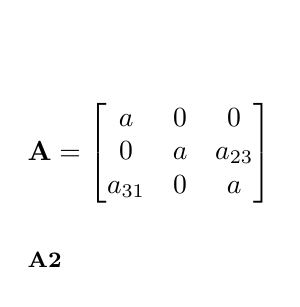
\begin{tikzpicture}[inner sep=0pt,outer sep=0pt]
\node[inner sep=0pt] (matA) {$\mathbf{A}=\begin{bmatrix}
a      & 0   & 0\\
0      & a   & a_{23}\\
a_{31} & 0   & a
\end{bmatrix}$};
\useasboundingbox (-0.5\cellwd,-45.35pt) rectangle (0.5\cellwd,45.35pt);
\node[overlay,anchor=south west,font=\bfseries\footnotesize,xshift=\labxshiftB,yshift=3.91pt] at (current bounding box.south west) {A2};
\end{tikzpicture}
\end{minipage}
&
\begin{minipage}[c]{\cellwd}
\centering
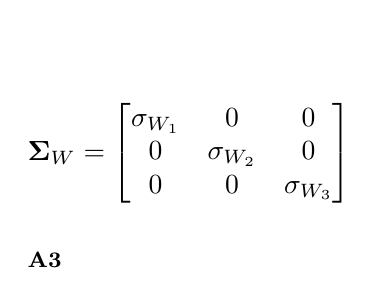
\begin{tikzpicture}[inner sep=0pt,outer sep=0pt]
\node[inner sep=0pt] (matSW) {$\mathbf{\Sigma}_W=\begin{bmatrix}
\sigma_{W_1}&0&0\\0&\sigma_{W_2}&0\\0&0&\sigma_{W_3}
\end{bmatrix}$};
\useasboundingbox (-0.5\cellwd,-45.35pt) rectangle (0.5\cellwd,45.35pt);
\node[overlay,anchor=south west,font=\bfseries\footnotesize,xshift=\labxshiftB,yshift=3.91pt] at (current bounding box.south west) {A3};
\end{tikzpicture}
\end{minipage}
\end{tabular}
\vspace{6pt}\hrule height 0.6pt\vspace{6pt}\nointerlineskip   % Divider 1
% --- Row A ---
\renewcommand{\thesubfigure}{B1}\phantomsubcaption\label{fig:mediator_B1}
\renewcommand{\thesubfigure}{B2}\phantomsubcaption\label{fig:mediator_B2}
\renewcommand{\thesubfigure}{B3}\phantomsubcaption\label{fig:mediator_B3}
\begin{tabular}{c@{\hspace{6pt}}|@{\hspace{6pt}}c@{\hspace{6pt}}|@{\hspace{6pt}}c}
\begin{minipage}[b]{\cellwd}
\centering
\begin{tikzpicture}[inner sep=0pt,outer sep=0pt]
\node[inner sep=0pt] (imgA1) {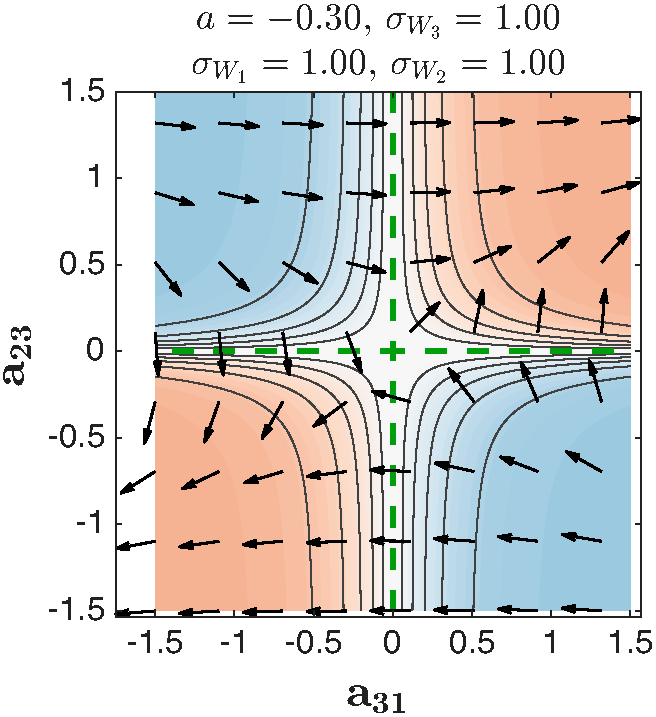
\includegraphics[width=\linewidth]{figures/topo_3node_mediator_figures/B1.pdf}};
\node[overlay,anchor=south west,font=\bfseries\footnotesize,xshift=-3.26pt,yshift=0.58pt] at (imgA1.south west) {B1};
\end{tikzpicture}
\end{minipage}
&
\begin{minipage}[b]{\cellwd}
\centering
\begin{tikzpicture}[inner sep=0pt,outer sep=0pt]
\node[inner sep=0pt] (imgA2) {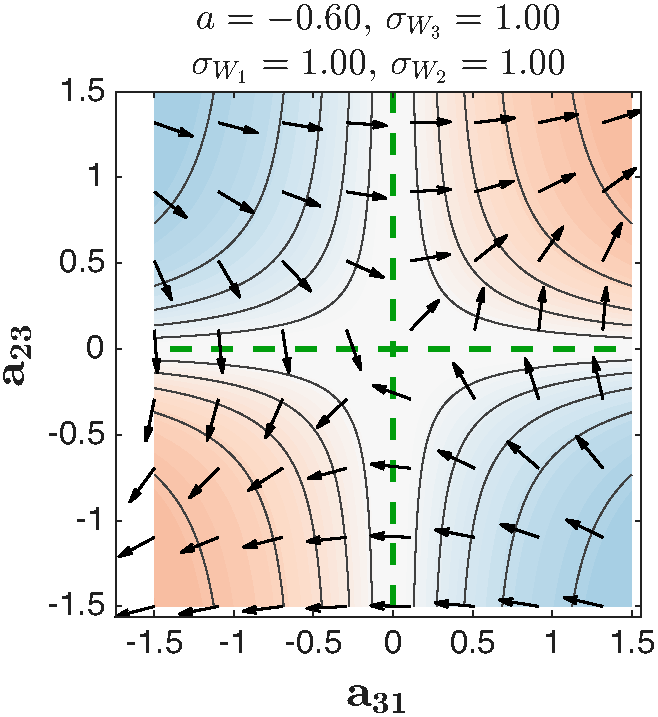
\includegraphics[width=\linewidth]{figures/topo_3node_mediator_figures/B2.pdf}};
\node[overlay,anchor=south west,font=\bfseries\footnotesize,xshift=\labxshiftB,yshift=0.58pt] at (imgA2.south west) {B2};
\end{tikzpicture}
\end{minipage}
&
\begin{minipage}[b]{\cellwd}
\centering
\begin{tikzpicture}[inner sep=0pt,outer sep=0pt]
\node[inner sep=0pt] (imgA3) {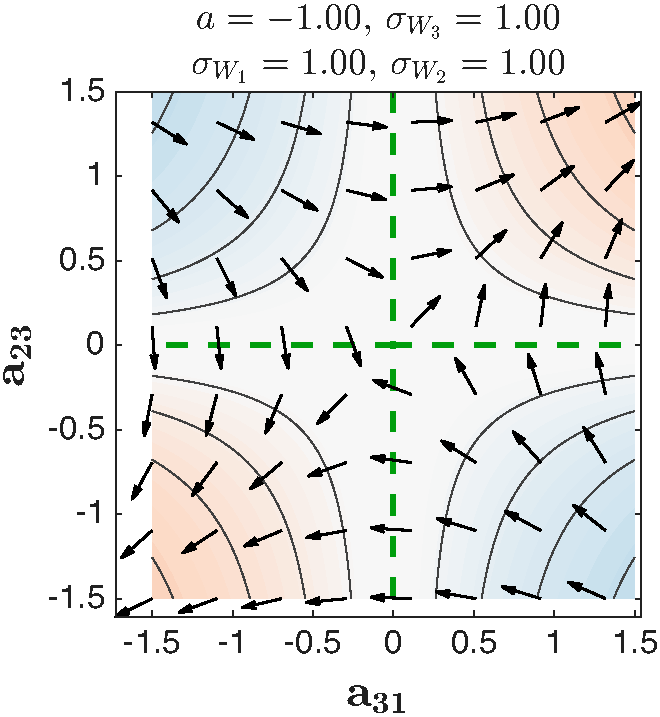
\includegraphics[width=\linewidth]{figures/topo_3node_mediator_figures/B3.pdf}};
\node[overlay,anchor=south west,font=\bfseries\footnotesize,xshift=\labxshiftB,yshift=0.58pt] at (imgA3.south west) {B3};
\end{tikzpicture}
\end{minipage}
\end{tabular}
\par
\vspace{6pt}\hrule height 0.6pt\vspace{6pt}\nointerlineskip   % Divider 2
% --- Row B ---
\renewcommand{\thesubfigure}{C1}\phantomsubcaption\label{fig:mediator_C1}
\renewcommand{\thesubfigure}{C2}\phantomsubcaption\label{fig:mediator_C2}
\renewcommand{\thesubfigure}{C3}\phantomsubcaption\label{fig:mediator_C3}
\begin{tabular}{c@{\hspace{6pt}}|@{\hspace{6pt}}c@{\hspace{6pt}}|@{\hspace{6pt}}c}
\begin{minipage}[b]{\cellwd}
\centering
\begin{tikzpicture}[inner sep=0pt,outer sep=0pt]
\node[inner sep=0pt] (imgB1) {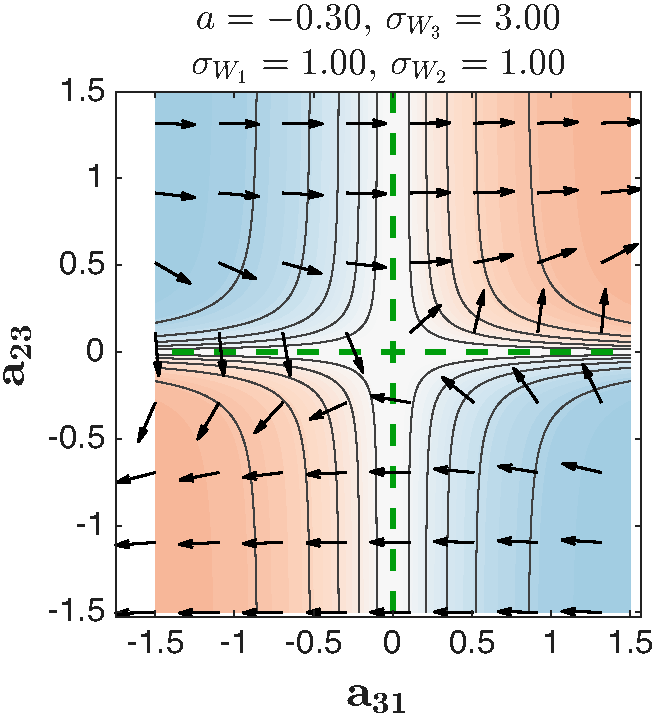
\includegraphics[width=\linewidth]{figures/topo_3node_mediator_figures/C1.pdf}};
\node[overlay,anchor=south west,font=\bfseries\footnotesize,xshift=-3.26pt,yshift=0.58pt] at (imgB1.south west) {C1};
\end{tikzpicture}
\end{minipage}
&
\begin{minipage}[b]{\cellwd}
\centering
\begin{tikzpicture}[inner sep=0pt,outer sep=0pt]
\node[inner sep=0pt] (imgB2) {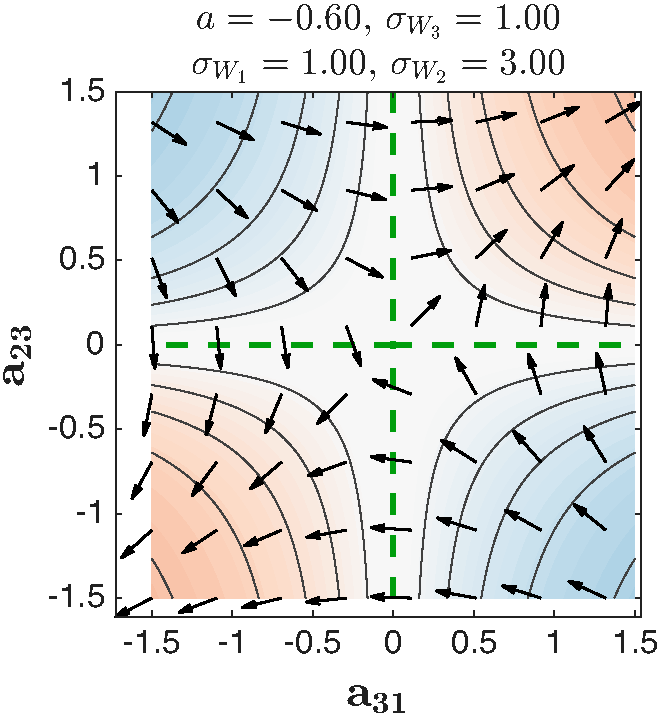
\includegraphics[width=\linewidth]{figures/topo_3node_mediator_figures/C2.pdf}};
\node[overlay,anchor=south west,font=\bfseries\footnotesize,xshift=\labxshiftB,yshift=0.58pt] at (imgB2.south west) {C2};
\end{tikzpicture}
\end{minipage}
&
\begin{minipage}[b]{\cellwd}
\centering
\begin{tikzpicture}[inner sep=0pt,outer sep=0pt]
\node[inner sep=0pt] (imgB3) {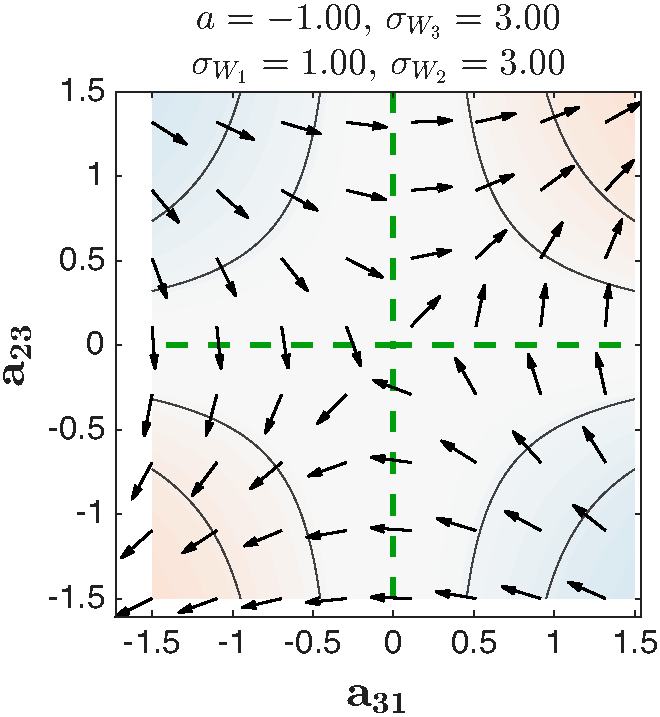
\includegraphics[width=\linewidth]{figures/topo_3node_mediator_figures/C3.pdf}};
\node[overlay,anchor=south west,font=\bfseries\footnotesize,xshift=\labxshiftB,yshift=0.58pt] at (imgB3.south west) {C3};
\end{tikzpicture}
\end{minipage}
\end{tabular}

\vspace{6pt}\hrule height 0.6pt\vspace{6pt}\nointerlineskip   % Divider 3
% --- colorbar (spans \rowwd) ---
\includegraphics[width=\rowwd]{figures/topo_3node_mediator_figures/colorbar.pdf}
\par
\vspace{3pt}
\end{minipage}%
}}
\end{figure}

% caption OUTSIDE the float; \addtocounter rolls back the phantomsubcaption bump
\addtocounter{figure}{-1}
\captionof{figure}{Mediator network.
Each panel is a contour/vector field plot of equation~(\ref{eq:rho21_mediator_main}) for
$\rho_{21}$ as a function of the mediation path coefficients $a_{31}$ and
$a_{23}$, over $a_{31},a_{23}\in[-1.5,1.5]$, for the combination of the
common self-connection $a$, $\sigma_{W_2}$, and $\sigma_{W_3}$ shown in
each panel's title ($\sigma_{W_1}=1$ throughout); $a$ strengthens across
the three columns ($a=-0.3,-0.6,-1.0$).
Arrows show the gradient direction of $\rho_{21}$.
Color encodes $\rho_{21}$ on a diverging scale from $-1$ (blue) through white
to $+1$ (red); values with $|\rho_{21}|<0.05$ are shown in white.
The dashed green lines mark $\rho_{21}=0$ exactly, forming a cross along
$a_{31}=0$ and $a_{23}=0$, where the correlation vanishes.}
\label{fig:rho21_mediator}

\vspace{6pt}
From equation~\ref{eq:rho21_mediator_main}, we see that the
numerator $a_{31}\,a_{23}\,\sigma_{W_1}$ is the product of
the two mediation path coefficients, weighted by the noise
variance of the source node~1 --- the continuous-time
dynamical analog of the Sobel test statistic \citep{Sobel1982}.
Just as the Sobel test quantifies an indirect effect as the
product of two path coefficients, our formula shows that the
mediated correlation is nonzero if and only if both
$a_{31}\neq0$ and $a_{23}\neq0$, and its sign matches the
sign of $a_{31}a_{23}$.
Two links of the same sign produce a positive correlation,
links of opposite signs a negative correlation.
The denominator makes explicit a feature that classical
mediation analysis treats as a nuisance.
The magnitude of the mediated correlation also depends on the
self-connection strength $a$ and the noise variances
$\sigma_{W_2}$ and $\sigma_{W_3}$, which scale the background
variance of nodes~2 and~3 against which the mediated influence from node~1 to node~2 must prevail (Figure~\ref{fig:rho21_mediator}).

% ============================================================
\subsection*{Two-Way Mediator}
% ============================================================

The two-way mediator network
(Figure~\ref{fig:rho21_mediator2way}\hyperref[fig:mediator2way_A1]{.A1})
extends the one-way mediator by adding returning connections. Node~1 and node~3 are reciprocally connected, as are node~2
and node~3, with no direct connection between nodes~1 and~2.
Writing $s=a_{13}a_{31}+a_{23}a_{32}$, the determinant factors
as $|\mathbf{K}|=16a^2\bigl(s-a^2\bigr)\bigl(s-4a^2\bigr)$.
Hurwitz stability requires $s<a^2$, together with $a<0$.
Under this condition both bracketed factors are negative, so
$|\mathbf{K}|>0$ throughout the stability region
(Figure~\ref{fig:rho21_mediator2way}).
Solving the Lyapunov equation for this two-way mediator
% Headline result: two-way mediator rho_21, derived in Appendix D.
network yields (\hyperref[app:appD]{Appendix~D},
equation~\ref{eq:rho21_mediator2way}),
\begin{equation}
\rho_{21} = \frac{N_{21}}{\sqrt{D_{11}\,D_{22}}},
\label{eq:rho21_med2way_main}
\end{equation}
where the numerator and denominator components are
\begin{align}
N_{21} &= \bigl(2a^2a_{23}a_{31} + a_{13}a_{23}a_{31}^2
          - 2a_{23}^2a_{31}a_{32}\bigr)\sigma_{W_1} \notag\\
&\quad+ \bigl(2a^2a_{13}a_{32} - 2a_{13}^2a_{31}a_{32}
          + a_{13}a_{23}a_{32}^2\bigr)\sigma_{W_2} \notag\\
&\quad+ \bigl(4a^2a_{13}a_{23} - a_{13}^2a_{23}a_{31}
          - a_{13}a_{23}^2a_{32}\bigr)\sigma_{W_3},
\label{eq:N21_med2way_main}\\[4pt]
D_{11} &= \bigl(8a^4 - 6a^2a_{13}a_{31} - 10a^2a_{23}a_{32}
          + a_{13}^2a_{31}^2 + 2a_{23}^2a_{32}^2\bigr)\sigma_{W_1}
          + 3a_{13}^2a_{32}^2\,\sigma_{W_2} \notag\\
&\quad+ \bigl(4a^2a_{13}^2 - a_{13}^3a_{31}
          - a_{13}^2a_{23}a_{32}\bigr)\sigma_{W_3},
\label{eq:D11_med2way_main}\\[4pt]
D_{22} &= 3a_{23}^2a_{31}^2\,\sigma_{W_1}
          + \bigl(8a^4 - 10a^2a_{13}a_{31} - 6a^2a_{23}a_{32}
          + 2a_{13}^2a_{31}^2 + a_{23}^2a_{32}^2\bigr)\sigma_{W_2} \notag\\
&\quad+ \bigl(4a^2a_{23}^2 - a_{23}^3a_{32}
          - a_{13}a_{23}^2a_{31}\bigr)\sigma_{W_3}.
\label{eq:D22_med2way_main}
\end{align}

A distinctive feature of the two-way mediator network, relative to its
one-way counterpart, is that all three noise variances now
appear in the numerator $N_{21}$.
This is because, with the "returning" connections $a_{13}$ and
$a_{32}$ present, fluctuations originating at any of the three
nodes can propagate to both node~1 and node~2, so every noise
source contributes to their covariance.
In the one-way mediator, by contrast, only $\sigma_{W_1}$
appears in the numerator of equation~(\ref{eq:rho21_mediator_main}).
Setting $a_{13}=a_{32}=0$ (removing the return connections and
leaving only the one-way path $1\to3\to2$) recovers the one-way
mediator network (see Figure~\ref{fig:rho21_mediator2way}\hyperref[fig:mediator2way_B1]{.B1})

% ============================================================
% Two-way mediator figure -- individual-panel template (produced per
% tasks/stage3_tasks_plot_networks/stage3_topo_x-node_figure_template_instructions.md).
% Panels exported by
% scripts/plot_networks/plot_topo_3node_mediator_2way_subplot.m to
% figures/topo_3node_mediator_2way_figures/. Two subplot rows (A/B); no row C.
% Panel mapping preserves the original 6 (a13,a32,a,sigma_W3) combinations and
% reading order (1->A1 ... 6->B3) -- see script header for why this topology
% does not split into a clean 3+3 row contrast.
% ============================================================
\begin{figure}[H]
\centering
{\setlength{\fboxrule}{0.6pt}\setlength{\arrayrulewidth}{0.6pt}%
\fbox{%
\begin{minipage}{\dimexpr\textwidth-2\fboxsep-2\fboxrule\relax}
\centering
\setlength{\cellwd}{\dimexpr(0.95\linewidth-12pt)/3\relax}
\setlength{\rowwd}{\dimexpr3\cellwd+12pt\relax}
\setlength{\labxshiftB}{-0.26pt}
\vspace{3pt}
% --- title ---
{\normalsize\textbf{$\rho_{21}$ as a function of $a_{31}$ and $a_{23}$ (two-way mediator)}}\par
\vspace{6pt}\hrule height 0.6pt\vspace{6pt}\nointerlineskip   % Divider 4
% --- structure strip: diagram | A | Sigma_W ---
% --- structure strip labels A1-A3 -- see dyad figure's comment
% for the label mechanism.
\renewcommand{\thesubfigure}{A1}
\phantomsubcaption\label{fig:mediator2way_A1}
\renewcommand{\thesubfigure}{A2}
\phantomsubcaption\label{fig:mediator2way_A2}
\renewcommand{\thesubfigure}{A3}
\phantomsubcaption\label{fig:mediator2way_A3}
\begin{tabular}{c@{\hspace{6pt}}|@{\hspace{6pt}}c@{\hspace{6pt}}|@{\hspace{6pt}}c}
\begin{minipage}[c]{\cellwd}
\centering
\def\a{1.0 cm}
\def\nodeSize{0.7}
\def\r{0.5*\nodeSize cm}
\begin{tikzpicture}[inner sep=0pt,outer sep=0pt]
\node[inner sep=0pt] (mediator2wayDiagram) {%
\begin{tikzpicture}[
    >={Stealth[length=3mm,width=2mm]},
    every node/.style={circle,draw,
        minimum size=\nodeSize cm}]
\node (1) at (-\a,0)          {1};
\node (2) at (\a,0)           {2};
\node (3) at (0,{sqrt(3)*\a}) {3};
\draw[->] (1) to[bend left=12]  (3);
\draw[->] (3) to[bend left=12]  (1);
\draw[->] (3) to[bend left=12]  (2);
\draw[->] (2) to[bend left=12]  (3);
\selfloop{1}{1}
\selfloop{2}{2}
\selfloop{3}{3}
\end{tikzpicture}%
};
\useasboundingbox (-0.5\cellwd,-45.35pt) rectangle (0.5\cellwd,45.35pt);
\node[overlay,anchor=south west,font=\bfseries\footnotesize,xshift=-3.26pt,yshift=3.91pt] at (current bounding box.south west) {A1};
\end{tikzpicture}
\end{minipage}
&
\begin{minipage}[c]{\cellwd}
\centering
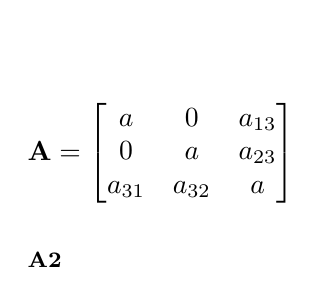
\begin{tikzpicture}[inner sep=0pt,outer sep=0pt]
\node[inner sep=0pt] (matA) {$\mathbf{A}=\begin{bmatrix}
a      & 0      & a_{13}\\
0      & a      & a_{23}\\
a_{31} & a_{32} & a
\end{bmatrix}$};
\useasboundingbox (-0.5\cellwd,-45.35pt) rectangle (0.5\cellwd,45.35pt);
\node[overlay,anchor=south west,font=\bfseries\footnotesize,xshift=\labxshiftB,yshift=3.91pt] at (current bounding box.south west) {A2};
\end{tikzpicture}
\end{minipage}
&
\begin{minipage}[c]{\cellwd}
\centering
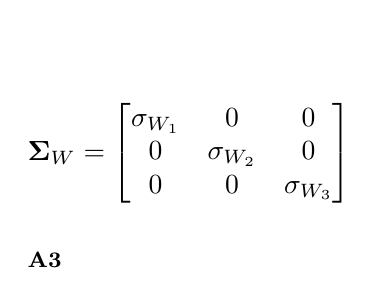
\begin{tikzpicture}[inner sep=0pt,outer sep=0pt]
\node[inner sep=0pt] (matSW) {$\mathbf{\Sigma}_W=\begin{bmatrix}
\sigma_{W_1}&0&0\\0&\sigma_{W_2}&0\\0&0&\sigma_{W_3}
\end{bmatrix}$};
\useasboundingbox (-0.5\cellwd,-45.35pt) rectangle (0.5\cellwd,45.35pt);
\node[overlay,anchor=south west,font=\bfseries\footnotesize,xshift=\labxshiftB,yshift=3.91pt] at (current bounding box.south west) {A3};
\end{tikzpicture}
\end{minipage}
\end{tabular}
\vspace{6pt}\hrule height 0.6pt\vspace{6pt}\nointerlineskip   % Divider 1
% --- Row A ---
\renewcommand{\thesubfigure}{B1}\phantomsubcaption\label{fig:mediator2way_B1}
\renewcommand{\thesubfigure}{B2}\phantomsubcaption\label{fig:mediator2way_B2}
\renewcommand{\thesubfigure}{B3}\phantomsubcaption\label{fig:mediator2way_B3}
\begin{tabular}{c@{\hspace{6pt}}|@{\hspace{6pt}}c@{\hspace{6pt}}|@{\hspace{6pt}}c}
\begin{minipage}[b]{\cellwd}
\centering
\begin{tikzpicture}[inner sep=0pt,outer sep=0pt]
\node[inner sep=0pt] (imgA1) {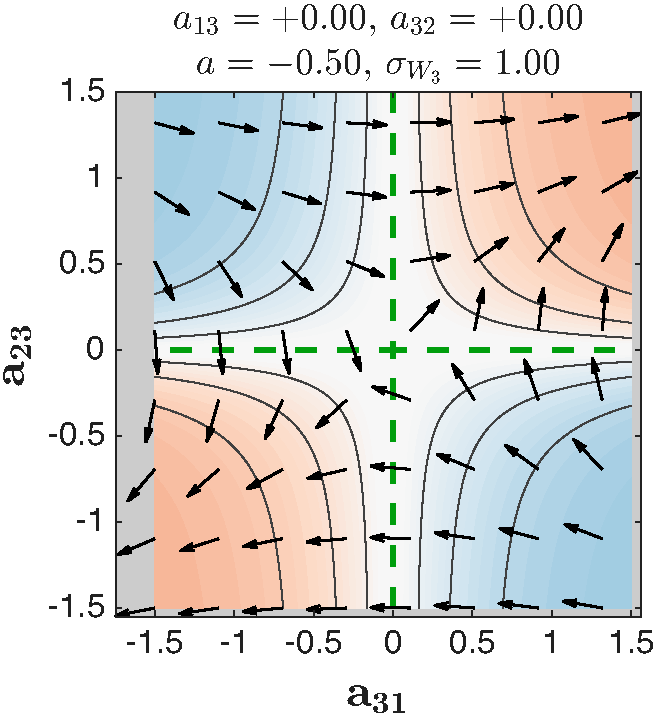
\includegraphics[width=\linewidth]{figures/topo_3node_mediator_2way_figures/B1.pdf}};
\node[overlay,anchor=south west,font=\bfseries\footnotesize,xshift=-3.26pt,yshift=0.58pt] at (imgA1.south west) {B1};
\end{tikzpicture}
\end{minipage}
&
\begin{minipage}[b]{\cellwd}
\centering
\begin{tikzpicture}[inner sep=0pt,outer sep=0pt]
\node[inner sep=0pt] (imgA2) {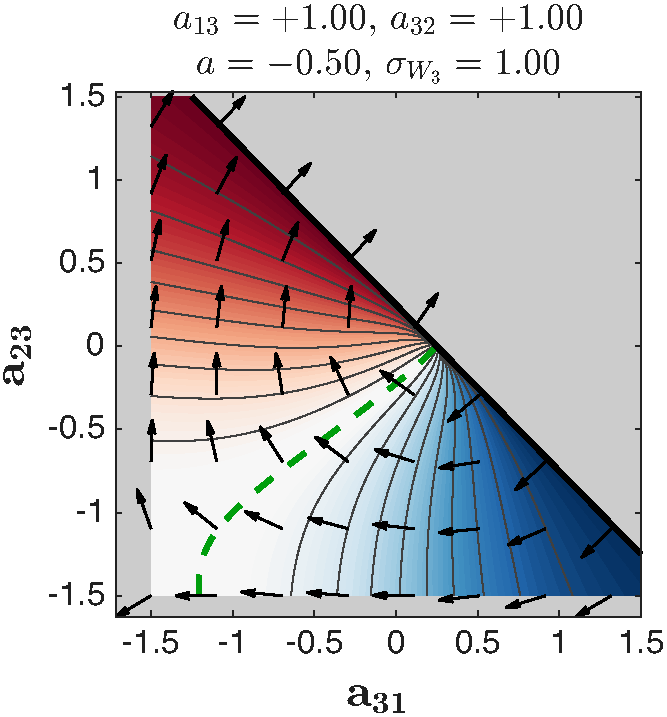
\includegraphics[width=\linewidth]{figures/topo_3node_mediator_2way_figures/B2.pdf}};
\node[overlay,anchor=south west,font=\bfseries\footnotesize,xshift=\labxshiftB,yshift=0.58pt] at (imgA2.south west) {B2};
\end{tikzpicture}
\end{minipage}
&
\begin{minipage}[b]{\cellwd}
\centering
\begin{tikzpicture}[inner sep=0pt,outer sep=0pt]
\node[inner sep=0pt] (imgA3) {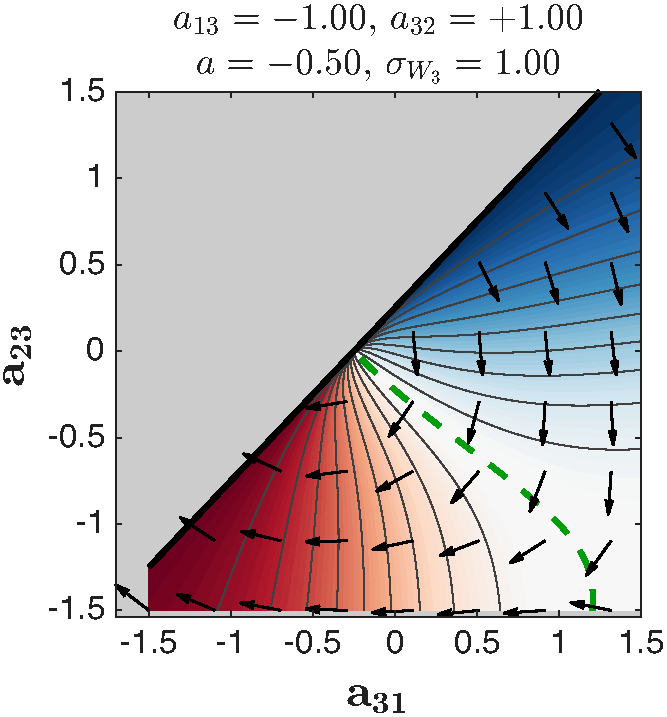
\includegraphics[width=\linewidth]{figures/topo_3node_mediator_2way_figures/B3.pdf}};
\node[overlay,anchor=south west,font=\bfseries\footnotesize,xshift=\labxshiftB,yshift=0.58pt] at (imgA3.south west) {B3};
\end{tikzpicture}
\end{minipage}
\end{tabular}
\par
\vspace{6pt}\hrule height 0.6pt\vspace{6pt}\nointerlineskip   % Divider 2
% --- Row B ---
\renewcommand{\thesubfigure}{C1}\phantomsubcaption\label{fig:mediator2way_C1}
\renewcommand{\thesubfigure}{C2}\phantomsubcaption\label{fig:mediator2way_C2}
\renewcommand{\thesubfigure}{C3}\phantomsubcaption\label{fig:mediator2way_C3}
\begin{tabular}{c@{\hspace{6pt}}|@{\hspace{6pt}}c@{\hspace{6pt}}|@{\hspace{6pt}}c}
\begin{minipage}[b]{\cellwd}
\centering
\begin{tikzpicture}[inner sep=0pt,outer sep=0pt]
\node[inner sep=0pt] (imgB1) {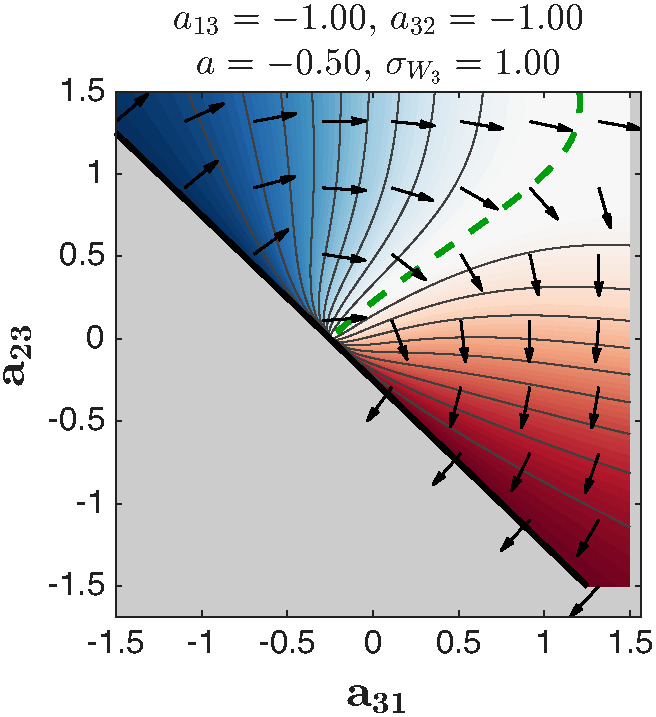
\includegraphics[width=\linewidth]{figures/topo_3node_mediator_2way_figures/C1.pdf}};
\node[overlay,anchor=south west,font=\bfseries\footnotesize,xshift=-3.26pt,yshift=0.58pt] at (imgB1.south west) {C1};
\end{tikzpicture}
\end{minipage}
&
\begin{minipage}[b]{\cellwd}
\centering
\begin{tikzpicture}[inner sep=0pt,outer sep=0pt]
\node[inner sep=0pt] (imgB2) {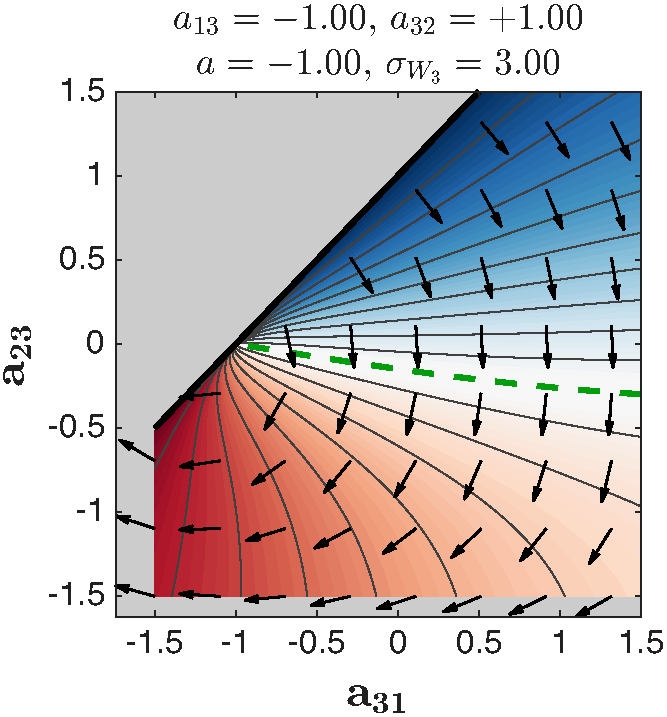
\includegraphics[width=\linewidth]{figures/topo_3node_mediator_2way_figures/C2.pdf}};
\node[overlay,anchor=south west,font=\bfseries\footnotesize,xshift=\labxshiftB,yshift=0.58pt] at (imgB2.south west) {C2};
\end{tikzpicture}
\end{minipage}
&
\begin{minipage}[b]{\cellwd}
\centering
\begin{tikzpicture}[inner sep=0pt,outer sep=0pt]
\node[inner sep=0pt] (imgB3) {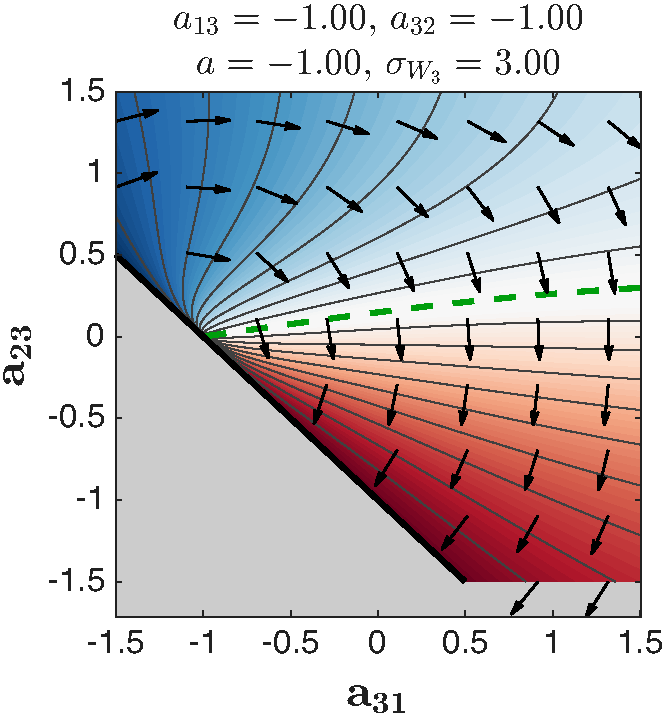
\includegraphics[width=\linewidth]{figures/topo_3node_mediator_2way_figures/C3.pdf}};
\node[overlay,anchor=south west,font=\bfseries\footnotesize,xshift=\labxshiftB,yshift=0.58pt] at (imgB3.south west) {C3};
\end{tikzpicture}
\end{minipage}
\end{tabular}

\vspace{6pt}\hrule height 0.6pt\vspace{6pt}\nointerlineskip   % Divider 3
% --- colorbar (spans \rowwd) ---
\includegraphics[width=\rowwd]{figures/topo_3node_mediator_2way_figures/colorbar.pdf}
\par

\vspace{3pt}
\end{minipage}%
}}
\end{figure}

% caption OUTSIDE the float; \addtocounter rolls back the phantomsubcaption bump
\addtocounter{figure}{-1}
\captionof{figure}{Two-way mediator network.
Each panel is a contour/vector field plot of equation~(\ref{eq:rho21_med2way_main}) for
$\rho_{21}$ over $a_{31},a_{23}\in[-1.5,1.5]$, with $a$ and
$\sigma_{W_3}$ shown in each panel's title.
Panel~\hyperref[fig:mediator2way_B1]{B1} sets $a_{13}=a_{32}=0$,
recovering the one-way mediator (Figure~\ref{fig:rho21_mediator})
exactly.
Panels~\hyperref[fig:mediator2way_B2]{B2}--\hyperref[fig:mediator2way_B3]{B3}
and~\hyperref[fig:mediator2way_C1]{C1} rotate $(a_{13},a_{32})$
through three sign quadrants at fixed magnitude 1, with
$a=-0.5$ and $\sigma_{W_1}=\sigma_{W_2}=\sigma_{W_3}=1$.
Panels~\hyperref[fig:mediator2way_C2]{C2}--\hyperref[fig:mediator2way_C3]{C3}
repeat those same $(a_{13},a_{32})$ pairs with $a=-1.0$ and
$\sigma_{W_3}=3$ instead, isolating how node~3's own dynamics ---
its self-connection and noise variance --- reshape the
correlation geometry for a fixed pair of return connections.
Color encodes $\rho_{21}$ on a diverging scale from $-1$ (blue) through white
to $+1$ (red); values with $|\rho_{21}|<0.05$ are shown in white.
The dashed green curve marks $\rho_{21}=0$ exactly.
The solid black curve is the Hurwitz stability boundary
$a_{13}a_{31}+a_{23}a_{32}=a^2$, with the grey region outside it
--- no steady state, $\rho_{21}$ undefined --- absent from
panel~\hyperref[fig:mediator2way_B1]{B1}, where $a_{13}=a_{32}=0$
makes the system stable everywhere.}
\label{fig:rho21_mediator2way}

% ============================================================
\subsection*{3-Cycle}
% ============================================================

The 3-cycle network
(Figure~\ref{fig:rho21_cycle}\hyperref[fig:cycle_A1]{.A1})
forms a directed ring. Node~1 drives node~3
($a_{31}\neq0$), node~3 drives node~2 ($a_{23}\neq0$),
and node~2 drives node~1 ($a_{12}\neq0$).
The feedback loop makes all three pairwise correlations
interdependent. The corresponding
$\mathbf{A}$ matrix
(Figure~\ref{fig:rho21_cycle}\hyperref[fig:cycle_A2]{.A2})
shows the equal-diagonal simplification $a=a_{11}=a_{22}=a_{33}$.
Writing $c=a_{12}a_{23}a_{31}$, the determinant factors as
$|\mathbf{K}|=8\bigl(8a^3-c\bigr)\bigl(a^3+c\bigr)$.
Hurwitz stability of the network requires a two-sided bound
$8a^3<c<-a^3$ (\hyperref[app:appD]{Appendix~D}).
Throughout this region both factors of $|\mathbf{K}|$ are
negative, so $|\mathbf{K}|>0$ and no sign prefactor is needed. The sign of each correlation is carried entirely by its
numerator. Solving the Lyapunov equation for this 3-cycle network yields
% Headline result: 3-cycle rho_21, derived in Appendix D.
(\hyperref[app:appD]{Appendix~D},
equation~\ref{eq:rho_cycle}),
\begin{equation}
\rho_{21} = \frac{N_{21}}{\sqrt{D_{11}\,D_{22}}},
\label{eq:rho21_cycle_main}
\end{equation}
where
\begin{align}
N_{21} &= \bigl(-2a^3a_{23}a_{31}+a_{12}a_{23}^2a_{31}^2\bigr)\sigma_{W_1}
        + \bigl(4a^4a_{12}+aa_{12}^2a_{23}a_{31}\bigr)\sigma_{W_2}
        + 3a^2a_{12}a_{23}^2\,\sigma_{W_3},
\label{eq:N21_cycle_main}\\[4pt]
D_{11} &= \bigl(8a^5+5a^2a_{12}a_{23}a_{31}\bigr)\sigma_{W_1}
        + \bigl(4a^3a_{12}^2+a_{12}^3a_{23}a_{31}\bigr)\sigma_{W_2}
        + 3aa_{12}^2a_{23}^2\,\sigma_{W_3},
\label{eq:D11_cycle_main}\\[4pt]
D_{22} &= \bigl(8a^5+5a^2a_{12}a_{23}a_{31}\bigr)\sigma_{W_2}
        + \bigl(4a^3a_{23}^2+a_{12}a_{23}^3a_{31}\bigr)\sigma_{W_3}
        + 3aa_{23}^2a_{31}^2\,\sigma_{W_1}.
\label{eq:D22_cycle_main}
\end{align}
The corresponding formulae for $\rho_{31}$ and $\rho_{32}$
follow the same pattern and are cyclically symmetric to
equation~(\ref{eq:rho21_cycle_main}), reflecting the rotational
symmetry of the network itself
(\hyperref[app:appD]{Appendix~D}). These expressions also reflect the feedback mechanism in this 3-cycle network topology. Although
each node sends a connection to only one other node, every
pairwise correlation depends on the strengths of all causal connections
($a_{12}$, $a_{23}$, $a_{31}$) and all three noise variances,
since influence injected anywhere on the ring eventually
reaches every node (Figure~\ref{fig:rho21_cycle}).

% ============================================================
% Cyclic network figure -- individual-panel template (produced per
% tasks/stage3_tasks_plot_networks/stage3_topo_x-node_figure_template_instructions.md).
% Panels exported by scripts/plot_networks/plot_topo_3node_cycle_subplot.m
% to figures/topo_3node_cycle_figures/. Two subplot rows (A/B); no row C.
% Panel mapping preserves the original 6 (a12,sigma_W3) combinations and
% reading order (1->A1 ... 6->B3) -- see script header for why this topology
% does not split into a clean 3+3 row contrast.
% ============================================================
\begin{figure}[H]
\centering
{\setlength{\fboxrule}{0.6pt}\setlength{\arrayrulewidth}{0.6pt}%
\fbox{%
\begin{minipage}{\dimexpr\textwidth-2\fboxsep-2\fboxrule\relax}
\centering
\setlength{\cellwd}{\dimexpr(0.95\linewidth-12pt)/3\relax}
\setlength{\rowwd}{\dimexpr3\cellwd+12pt\relax}
\setlength{\labxshiftB}{-0.26pt}
\vspace{3pt}
% --- title ---
{\normalsize\textbf{$\rho_{21}$ as a function of $a_{31}$ and $a_{23}$ (3-cycle)}}\par
\vspace{6pt}\hrule height 0.6pt\vspace{6pt}\nointerlineskip   % Divider 4
% --- structure strip: diagram | A | Sigma_W ---
% --- structure strip labels A1-A3 -- see dyad figure's comment
% for the label mechanism.
\renewcommand{\thesubfigure}{A1}
\phantomsubcaption\label{fig:cycle_A1}
\renewcommand{\thesubfigure}{A2}
\phantomsubcaption\label{fig:cycle_A2}
\renewcommand{\thesubfigure}{A3}
\phantomsubcaption\label{fig:cycle_A3}
\begin{tabular}{c@{\hspace{6pt}}|@{\hspace{6pt}}c@{\hspace{6pt}}|@{\hspace{6pt}}c}
\begin{minipage}[c]{\cellwd}
\centering
\def\a{1.0 cm}
\def\nodeSize{0.7}
\def\r{0.5*\nodeSize cm}
\begin{tikzpicture}[inner sep=0pt,outer sep=0pt]
\node[inner sep=0pt] (cycleDiagram) {%
\begin{tikzpicture}[
    >={Stealth[length=3mm,width=2mm]},
    every node/.style={circle,draw,
        minimum size=\nodeSize cm}]
\node (1) at (-\a,0)          {1};
\node (2) at (\a,0)           {2};
\node (3) at (0,{sqrt(3)*\a}) {3};
\draw[->] (2) to[bend left=12]  (1);
\draw[->] (3) to[bend left=12]  (2);
\draw[->] (1) to[bend left=12]  (3);
\selfloop{1}{1}
\selfloop{2}{2}
\selfloop{3}{3}
\end{tikzpicture}%
};
\useasboundingbox (-0.5\cellwd,-45.35pt) rectangle (0.5\cellwd,45.35pt);
\node[overlay,anchor=south west,font=\bfseries\footnotesize,xshift=-3.26pt,yshift=3.91pt] at (current bounding box.south west) {A1};
\end{tikzpicture}
\end{minipage}
&
\begin{minipage}[c]{\cellwd}
\centering
\begin{tikzpicture}[inner sep=0pt,outer sep=0pt]
\node[inner sep=0pt] (matA) {$\mathbf{A}=\begin{bmatrix}
a      & a_{12} & 0\\
0      & a      & a_{23}\\
a_{31} & 0      & a
\end{bmatrix}$};
\useasboundingbox (-0.5\cellwd,-45.35pt) rectangle (0.5\cellwd,45.35pt);
\node[overlay,anchor=south west,font=\bfseries\footnotesize,xshift=\labxshiftB,yshift=3.91pt] at (current bounding box.south west) {A2};
\end{tikzpicture}
\end{minipage}
&
\begin{minipage}[c]{\cellwd}
\centering
\begin{tikzpicture}[inner sep=0pt,outer sep=0pt]
\node[inner sep=0pt] (matSW) {$\mathbf{\Sigma}_W=\begin{bmatrix}
\sigma_{W_1}&0&0\\0&\sigma_{W_2}&0\\0&0&\sigma_{W_3}
\end{bmatrix}$};
\useasboundingbox (-0.5\cellwd,-45.35pt) rectangle (0.5\cellwd,45.35pt);
\node[overlay,anchor=south west,font=\bfseries\footnotesize,xshift=\labxshiftB,yshift=3.91pt] at (current bounding box.south west) {A3};
\end{tikzpicture}
\end{minipage}
\end{tabular}
\vspace{6pt}\hrule height 0.6pt\vspace{6pt}\nointerlineskip   % Divider 1
% --- Row A ---
\renewcommand{\thesubfigure}{B1}\phantomsubcaption\label{fig:cycle_B1}
\renewcommand{\thesubfigure}{B2}\phantomsubcaption\label{fig:cycle_B2}
\renewcommand{\thesubfigure}{B3}\phantomsubcaption\label{fig:cycle_B3}
\begin{tabular}{c@{\hspace{6pt}}|@{\hspace{6pt}}c@{\hspace{6pt}}|@{\hspace{6pt}}c}
\begin{minipage}[b]{\cellwd}
\centering
\begin{tikzpicture}[inner sep=0pt,outer sep=0pt]
\node[inner sep=0pt] (imgA1) {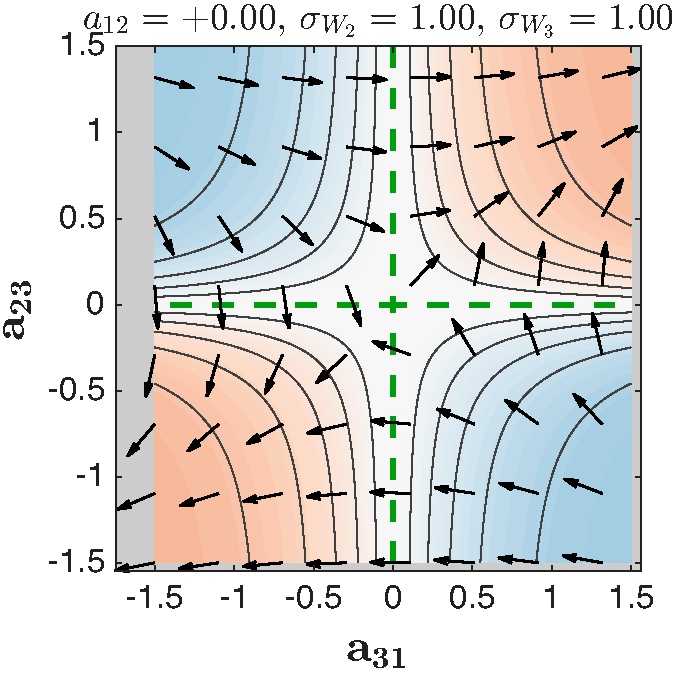
\includegraphics[width=\linewidth]{figures/topo_3node_cycle_figures/B1.pdf}};
\node[overlay,anchor=south west,font=\bfseries\footnotesize,xshift=-3.26pt,yshift=0.58pt] at (imgA1.south west) {B1};
\end{tikzpicture}
\end{minipage}
&
\begin{minipage}[b]{\cellwd}
\centering
\begin{tikzpicture}[inner sep=0pt,outer sep=0pt]
\node[inner sep=0pt] (imgA2) {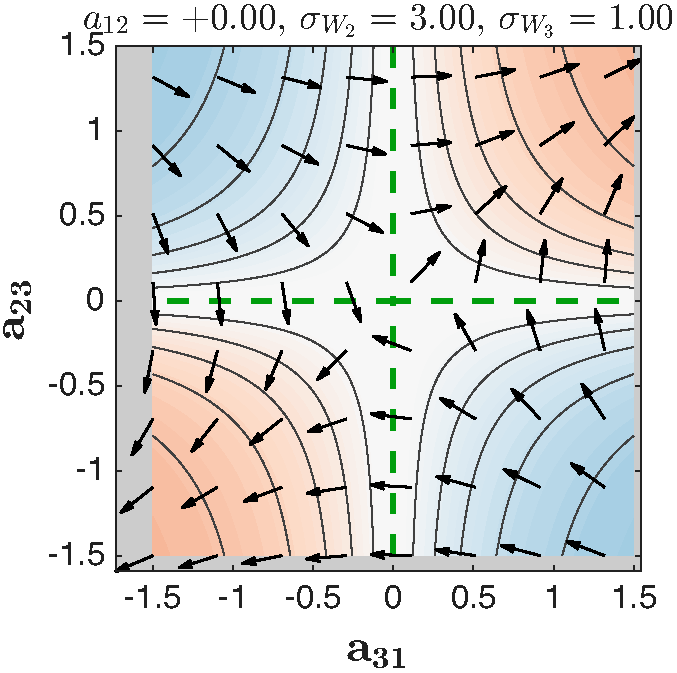
\includegraphics[width=\linewidth]{figures/topo_3node_cycle_figures/B2.pdf}};
\node[overlay,anchor=south west,font=\bfseries\footnotesize,xshift=\labxshiftB,yshift=0.58pt] at (imgA2.south west) {B2};
\end{tikzpicture}
\end{minipage}
&
\begin{minipage}[b]{\cellwd}
\centering
\begin{tikzpicture}[inner sep=0pt,outer sep=0pt]
\node[inner sep=0pt] (imgA3) {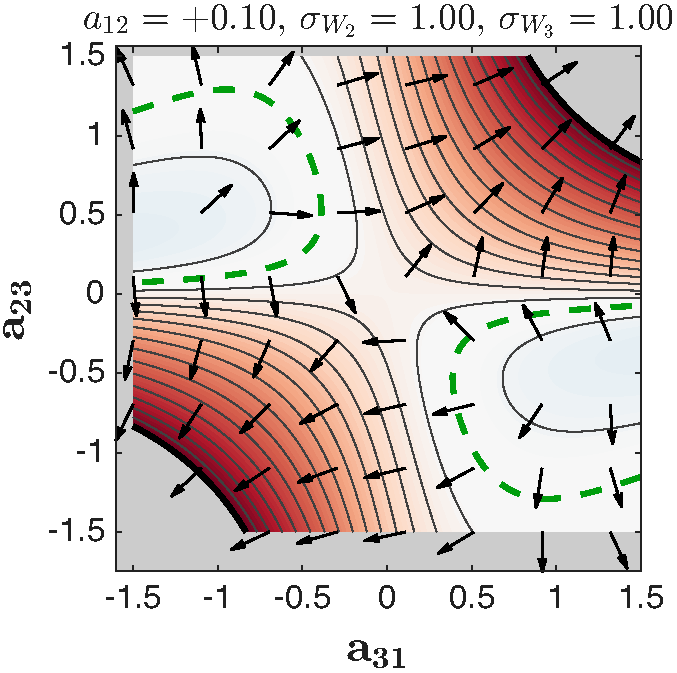
\includegraphics[width=\linewidth]{figures/topo_3node_cycle_figures/B3.pdf}};
\node[overlay,anchor=south west,font=\bfseries\footnotesize,xshift=\labxshiftB,yshift=0.58pt] at (imgA3.south west) {B3};
\end{tikzpicture}
\end{minipage}
\end{tabular}
\par
\vspace{6pt}\hrule height 0.6pt\vspace{6pt}\nointerlineskip   % Divider 2
% --- Row B ---
\renewcommand{\thesubfigure}{C1}\phantomsubcaption\label{fig:cycle_C1}
\renewcommand{\thesubfigure}{C2}\phantomsubcaption\label{fig:cycle_C2}
\renewcommand{\thesubfigure}{C3}\phantomsubcaption\label{fig:cycle_C3}
\begin{tabular}{c@{\hspace{6pt}}|@{\hspace{6pt}}c@{\hspace{6pt}}|@{\hspace{6pt}}c}
\begin{minipage}[b]{\cellwd}
\centering
\begin{tikzpicture}[inner sep=0pt,outer sep=0pt]
\node[inner sep=0pt] (imgB1) {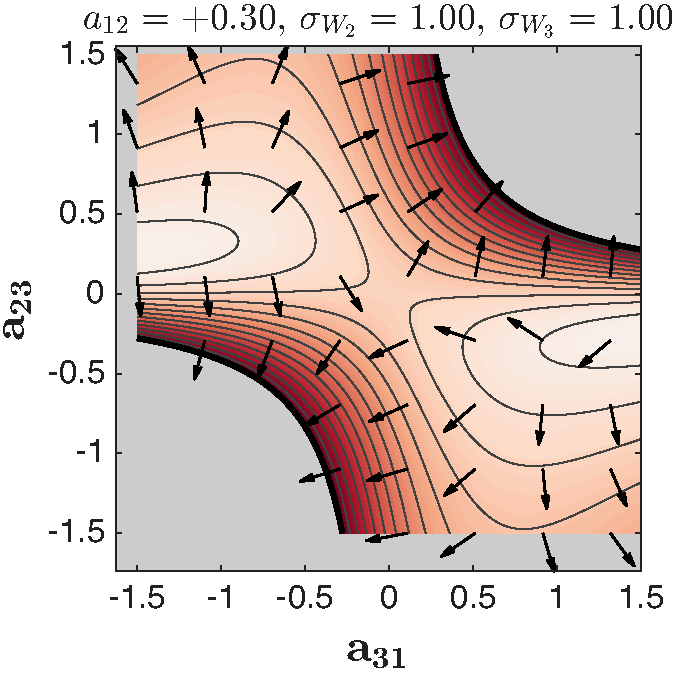
\includegraphics[width=\linewidth]{figures/topo_3node_cycle_figures/C1.pdf}};
\node[overlay,anchor=south west,font=\bfseries\footnotesize,xshift=-3.26pt,yshift=0.58pt] at (imgB1.south west) {C1};
\end{tikzpicture}
\end{minipage}
&
\begin{minipage}[b]{\cellwd}
\centering
\begin{tikzpicture}[inner sep=0pt,outer sep=0pt]
\node[inner sep=0pt] (imgB2) {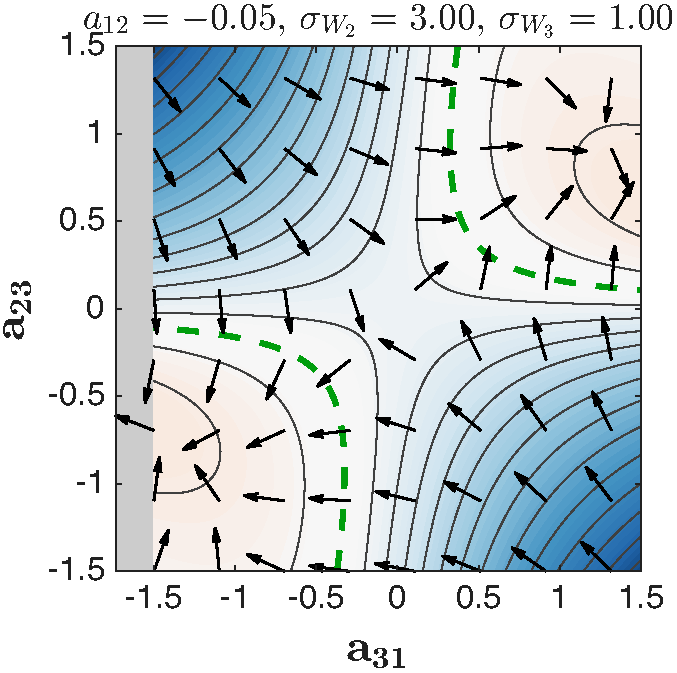
\includegraphics[width=\linewidth]{figures/topo_3node_cycle_figures/C2.pdf}};
\node[overlay,anchor=south west,font=\bfseries\footnotesize,xshift=\labxshiftB,yshift=0.58pt] at (imgB2.south west) {C2};
\end{tikzpicture}
\end{minipage}
&
\begin{minipage}[b]{\cellwd}
\centering
\begin{tikzpicture}[inner sep=0pt,outer sep=0pt]
\node[inner sep=0pt] (imgB3) {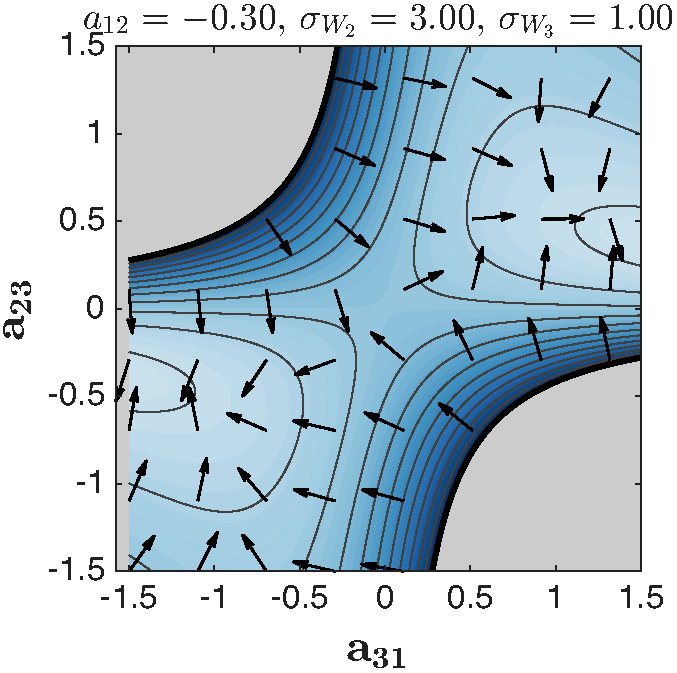
\includegraphics[width=\linewidth]{figures/topo_3node_cycle_figures/C3.pdf}};
\node[overlay,anchor=south west,font=\bfseries\footnotesize,xshift=\labxshiftB,yshift=0.58pt] at (imgB3.south west) {C3};
\end{tikzpicture}
\end{minipage}
\end{tabular}

\vspace{6pt}\hrule height 0.6pt\vspace{6pt}\nointerlineskip   % Divider 3
% --- colorbar (spans \rowwd) ---
\includegraphics[width=\rowwd]{figures/topo_3node_cycle_figures/colorbar.pdf}
\par

\vspace{3pt}
\end{minipage}%
}}
\end{figure}

% caption OUTSIDE the float; \addtocounter rolls back the phantomsubcaption bump
\addtocounter{figure}{-1}
\captionof{figure}{3-Cycle network.
Each panel is a contour/vector field plot of equation~(\ref{eq:rho21_cycle_main}) for
$\rho_{21}$ as a function of $a_{31}$ and $a_{23}$ (two of the three ring
edges), over $a_{31},a_{23}\in[-1.5,1.5]$, with $a=-0.5$ and
$\sigma_{W_1}=1$ fixed throughout; $a_{12}$ (the third ring edge),
$\sigma_{W_2}$, and $\sigma_{W_3}$ are indicated in each panel's title.
Color encodes $\rho_{21}$ on a diverging scale from $-1$ (blue) through white
to $+1$ (red); values with $|\rho_{21}|<0.05$ are shown in white.
The dashed green curve marks $\rho_{21}=0$ exactly.
The solid black curves are the Hurwitz stability boundaries
$a_{12}a_{23}a_{31}=8a^3$ and $=-a^3$; the grey region outside them is where
no steady state exists and $\rho_{21}$ is undefined.}
\label{fig:rho21_cycle}

\clearpage
% ============================================================
\subsection*{Moderator}
% ============================================================

The moderator network topology
(Figure~\ref{fig:rho21_moderator}\hyperref[fig:moderator_A1]{.A1})
combines elements from the dyad and confounder networks. Nodes~1
and~2 exert direct reciprocal influences on each other
($a_{12}\neq0$, $a_{21}\neq0$), and both also receive input
from a third node~3 ($a_{13}\neq0$, $a_{23}\neq0$). However, node~3 receives no input from nodes~1 or~2.
Here $a_{12}$, $a_{21}$, $a_{13}$, and $a_{23}$ are the four
causal influences forming the reciprocal pair and the common
driver (Figure~\ref{fig:rho21_moderator}\hyperref[fig:moderator_A2]{.A2}).
The determinant $|\mathbf{K}|=16a^2\bigl(a^2-a_{12}a_{21}\bigr)
\bigl(4a^2-a_{12}a_{21}\bigr)$ is strictly positive under
Hurwitz stability (\hyperref[app:appD]{Appendix~D}). Thus, the
sign of $\rho_{21}$ is carried entirely by its numerator
$N_{21}$ and no sign prefactor appears in $\rho_{21}$.
Solving the Lyapunov equation for this moderator network
% Headline result: moderator rho_21, derived in Appendix D.
yields the following formula for $\rho_{21}$ (\hyperref[app:appD]{Appendix~D},
equation~\ref{eq:rho21_moderator}),
\begin{equation}
\rho_{21} = \frac{N_{21}}{\sqrt{D_{11}\,D_{22}}},
\label{eq:rho21_moderator_main}
\end{equation}
where the numerator and denominator components are
\begin{align}
N_{21} &=
  (aa_{12}a_{21}^2-4a^3a_{21})\sigma_{W_1}
  +(aa_{12}^2a_{21}-4a^3a_{12})\sigma_{W_2} \notag\\
  &\quad+(-3aa_{12}a_{23}^2-3aa_{13}^2a_{21}
    +2a_{12}a_{13}a_{21}a_{23}
    +4a^2a_{13}a_{23})\sigma_{W_3},
\label{eq:N21_mod}\\[4pt]
D_{11} &=
  (8a^4-6a^2a_{12}a_{21}+a_{12}^2a_{21}^2)\sigma_{W_1}
  +(4a^2a_{12}^2-a_{12}^3a_{21})\sigma_{W_2} \notag\\
  &\quad+(4a^2a_{13}^2-6aa_{12}a_{13}a_{23}
    +3a_{12}^2a_{23}^2-a_{12}a_{13}^2a_{21})\sigma_{W_3},
\label{eq:D11_mod}\\[4pt]
D_{22} &=
  (8a^4-6a^2a_{12}a_{21}+a_{12}^2a_{21}^2)\sigma_{W_2}
  +(4a^2a_{21}^2-a_{12}a_{21}^3)\sigma_{W_1} \notag\\
  &\quad+(4a^2a_{23}^2-6aa_{13}a_{21}a_{23}
    +3a_{13}^2a_{21}^2-a_{12}a_{21}a_{23}^2)\sigma_{W_3}.
\label{eq:D22_mod}
\end{align}

Setting $a_{13}=a_{23}=0$ in
equations~(\ref{eq:N21_mod})--(\ref{eq:D22_mod}) immediately
recovers the formula for the dyadic network~(see Equation (\ref{eq:rho21_dyad})),
confirming the moderator network as a direct extension of
the dyadic case.
The $\sigma_{W_3}$ terms quantify the additional contribution
of the common driver to the correlation. They appear in both
the numerator and denominator, reshaping the correlation
surface even when the direct connections $a_{12}$ and $a_{21}$
are held fixed.
This has an important practical implication. The same pair of
directly connected nodes can exhibit substantially different
correlations depending on whether they have a common driver,
even if the direct connection strengths are identical.
The correlation structure observable from data therefore
reflects not just the direct connections but the entire
embedding of those connections within a larger causal network.

% ============================================================
% Moderator figure -- individual-panel template (produced per
% tasks/stage3_tasks_plot_networks/stage3_topo_x-node_figure_template_instructions.md).
% Panels exported by
% scripts/plot_networks/plot_topo_3node_moderator_subplot.m to
% figures/topo_3node_moderator_figures/. Two subplot rows (A/B); no row C.
% Panel mapping preserves the original 6 (a13,a23) combinations and reading
% order (1->A1 ... 6->B3) -- a, sigma_W1, sigma_W2, sigma_W3 are fixed across
% all panels here, so there is no row/column contrast to exploit.
% ============================================================
\begin{figure}[H]
\centering
{\setlength{\fboxrule}{0.6pt}\setlength{\arrayrulewidth}{0.6pt}%
\fbox{%
\begin{minipage}{\dimexpr\textwidth-2\fboxsep-2\fboxrule\relax}
\centering
\setlength{\cellwd}{\dimexpr(0.95\linewidth-12pt)/3\relax}
\setlength{\rowwd}{\dimexpr3\cellwd+12pt\relax}
\setlength{\labxshiftB}{-0.26pt}
\vspace{3pt}
% --- title ---
{\normalsize\textbf{$\rho_{21}$ as a function of $a_{12}$ and $a_{21}$ (moderator)}}\par
\vspace{6pt}\hrule height 0.6pt\vspace{6pt}\nointerlineskip   % Divider 4
% --- structure strip: diagram | A | Sigma_W ---
% --- structure strip labels A1-A3 -- see dyad figure's comment
% for the label mechanism.
\renewcommand{\thesubfigure}{A1}
\phantomsubcaption\label{fig:moderator_A1}
\renewcommand{\thesubfigure}{A2}
\phantomsubcaption\label{fig:moderator_A2}
\renewcommand{\thesubfigure}{A3}
\phantomsubcaption\label{fig:moderator_A3}
\begin{tabular}{c@{\hspace{6pt}}|@{\hspace{6pt}}c@{\hspace{6pt}}|@{\hspace{6pt}}c}
\begin{minipage}[c]{\cellwd}
\centering
\def\a{1.0 cm}
\def\nodeSize{0.7}
\def\r{0.5*\nodeSize cm}
\begin{tikzpicture}[inner sep=0pt,outer sep=0pt]
\node[inner sep=0pt] (moderatorDiagram) {%
\begin{tikzpicture}[
    >={Stealth[length=3mm,width=2mm]},
    every node/.style={circle,draw,
        minimum size=\nodeSize cm}]
\node (1) at (-\a,0)          {1};
\node (2) at (\a,0)           {2};
\node (3) at (0,{sqrt(3)*\a}) {3};
\draw[->] (1) to[bend left=12]  (2);
\draw[->] (2) to[bend left=12]  (1);
\draw[->] (3) to[bend right=12] (1);
\draw[->] (3) to[bend left=12]  (2);
\selfloop{1}{1}
\selfloop{2}{2}
\selfloop{3}{3}
\end{tikzpicture}%
};
\useasboundingbox (-0.5\cellwd,-45.35pt) rectangle (0.5\cellwd,45.35pt);
\node[overlay,anchor=south west,font=\bfseries\footnotesize,xshift=-3.26pt,yshift=3.91pt] at (current bounding box.south west) {A1};
\end{tikzpicture}
\end{minipage}
&
\begin{minipage}[c]{\cellwd}
\centering
\begin{tikzpicture}[inner sep=0pt,outer sep=0pt]
\node[inner sep=0pt] (matA) {$\mathbf{A}=\begin{bmatrix}
a      & a_{12} & a_{13}\\
a_{21} & a      & a_{23}\\
0      & 0      & a
\end{bmatrix}$};
\useasboundingbox (-0.5\cellwd,-45.35pt) rectangle (0.5\cellwd,45.35pt);
\node[overlay,anchor=south west,font=\bfseries\footnotesize,xshift=\labxshiftB,yshift=3.91pt] at (current bounding box.south west) {A2};
\end{tikzpicture}
\end{minipage}
&
\begin{minipage}[c]{\cellwd}
\centering
\begin{tikzpicture}[inner sep=0pt,outer sep=0pt]
\node[inner sep=0pt] (matSW) {$\mathbf{\Sigma}_W=\begin{bmatrix}
\sigma_{W_1}&0&0\\0&\sigma_{W_2}&0\\0&0&\sigma_{W_3}
\end{bmatrix}$};
\useasboundingbox (-0.5\cellwd,-45.35pt) rectangle (0.5\cellwd,45.35pt);
\node[overlay,anchor=south west,font=\bfseries\footnotesize,xshift=\labxshiftB,yshift=3.91pt] at (current bounding box.south west) {A3};
\end{tikzpicture}
\end{minipage}
\end{tabular}
\vspace{6pt}\hrule height 0.6pt\vspace{6pt}\nointerlineskip   % Divider 1
% --- Row A ---
\renewcommand{\thesubfigure}{B1}\phantomsubcaption\label{fig:moderator_B1}
\renewcommand{\thesubfigure}{B2}\phantomsubcaption\label{fig:moderator_B2}
\renewcommand{\thesubfigure}{B3}\phantomsubcaption\label{fig:moderator_B3}
\begin{tabular}{c@{\hspace{6pt}}|@{\hspace{6pt}}c@{\hspace{6pt}}|@{\hspace{6pt}}c}
\begin{minipage}[b]{\cellwd}
\centering
\begin{tikzpicture}[inner sep=0pt,outer sep=0pt]
\node[inner sep=0pt] (imgA1) {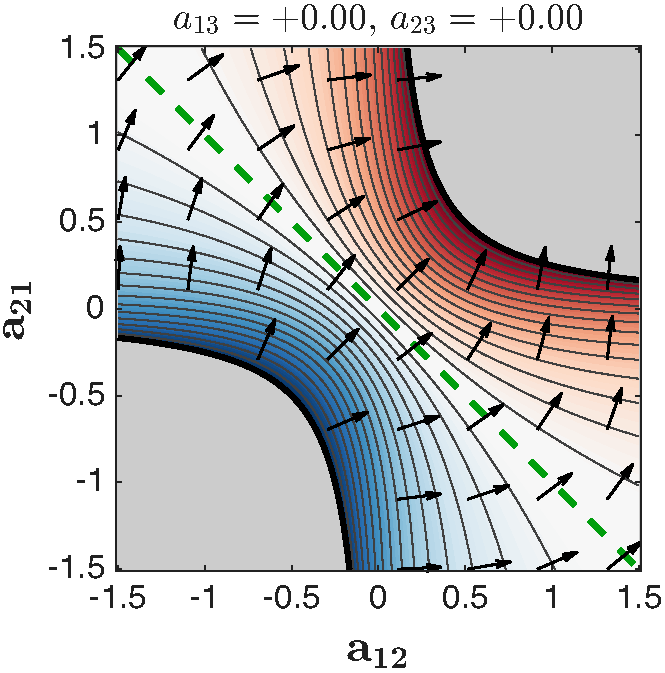
\includegraphics[width=\linewidth]{figures/topo_3node_moderator_figures/B1.pdf}};
\node[overlay,anchor=south west,font=\bfseries\footnotesize,xshift=-3.26pt,yshift=0.58pt] at (imgA1.south west) {B1};
\end{tikzpicture}
\end{minipage}
&
\begin{minipage}[b]{\cellwd}
\centering
\begin{tikzpicture}[inner sep=0pt,outer sep=0pt]
\node[inner sep=0pt] (imgA2) {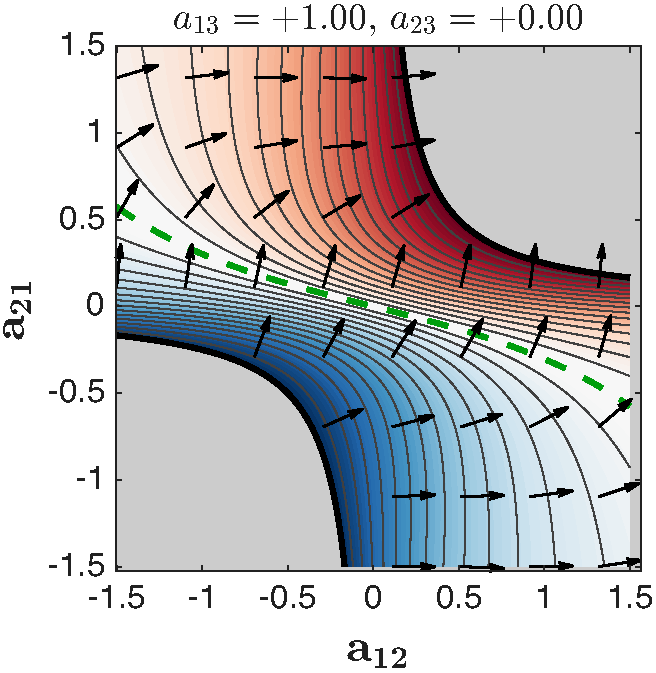
\includegraphics[width=\linewidth]{figures/topo_3node_moderator_figures/B2.pdf}};
\node[overlay,anchor=south west,font=\bfseries\footnotesize,xshift=\labxshiftB,yshift=0.58pt] at (imgA2.south west) {B2};
\end{tikzpicture}
\end{minipage}
&
\begin{minipage}[b]{\cellwd}
\centering
\begin{tikzpicture}[inner sep=0pt,outer sep=0pt]
\node[inner sep=0pt] (imgA3) {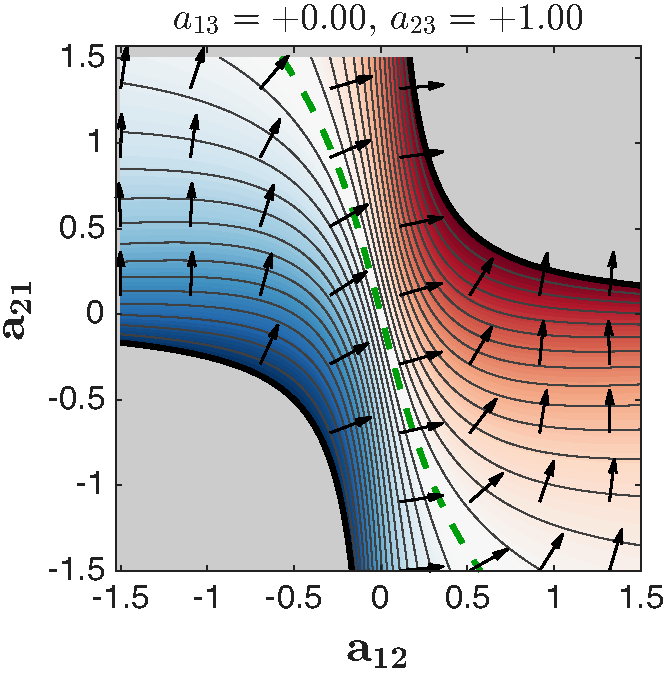
\includegraphics[width=\linewidth]{figures/topo_3node_moderator_figures/B3.pdf}};
\node[overlay,anchor=south west,font=\bfseries\footnotesize,xshift=\labxshiftB,yshift=0.58pt] at (imgA3.south west) {B3};
\end{tikzpicture}
\end{minipage}
\end{tabular}
\par
\vspace{6pt}\hrule height 0.6pt\vspace{6pt}\nointerlineskip   % Divider 2
% --- Row B ---
\renewcommand{\thesubfigure}{C1}\phantomsubcaption\label{fig:moderator_C1}
\renewcommand{\thesubfigure}{C2}\phantomsubcaption\label{fig:moderator_C2}
\renewcommand{\thesubfigure}{C3}\phantomsubcaption\label{fig:moderator_C3}
\begin{tabular}{c@{\hspace{6pt}}|@{\hspace{6pt}}c@{\hspace{6pt}}|@{\hspace{6pt}}c}
\begin{minipage}[b]{\cellwd}
\centering
\begin{tikzpicture}[inner sep=0pt,outer sep=0pt]
\node[inner sep=0pt] (imgB1) {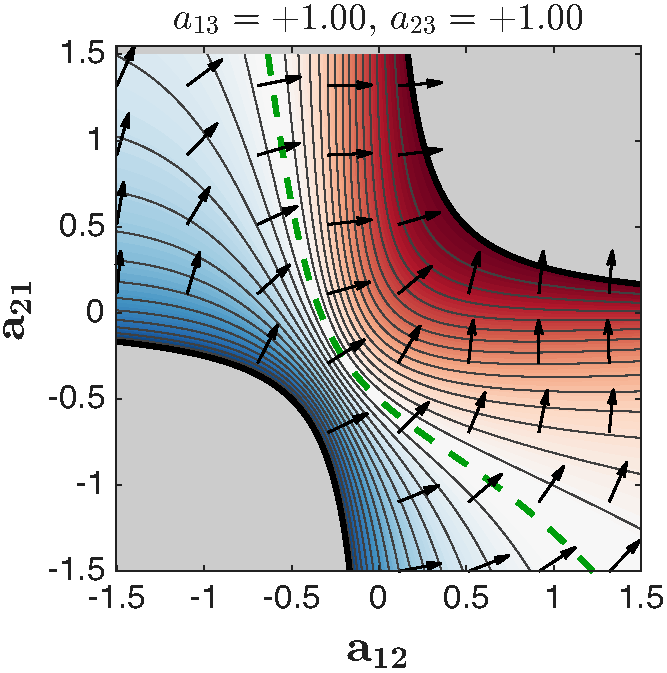
\includegraphics[width=\linewidth]{figures/topo_3node_moderator_figures/C1.pdf}};
\node[overlay,anchor=south west,font=\bfseries\footnotesize,xshift=-3.26pt,yshift=0.58pt] at (imgB1.south west) {C1};
\end{tikzpicture}
\end{minipage}
&
\begin{minipage}[b]{\cellwd}
\centering
\begin{tikzpicture}[inner sep=0pt,outer sep=0pt]
\node[inner sep=0pt] (imgB2) {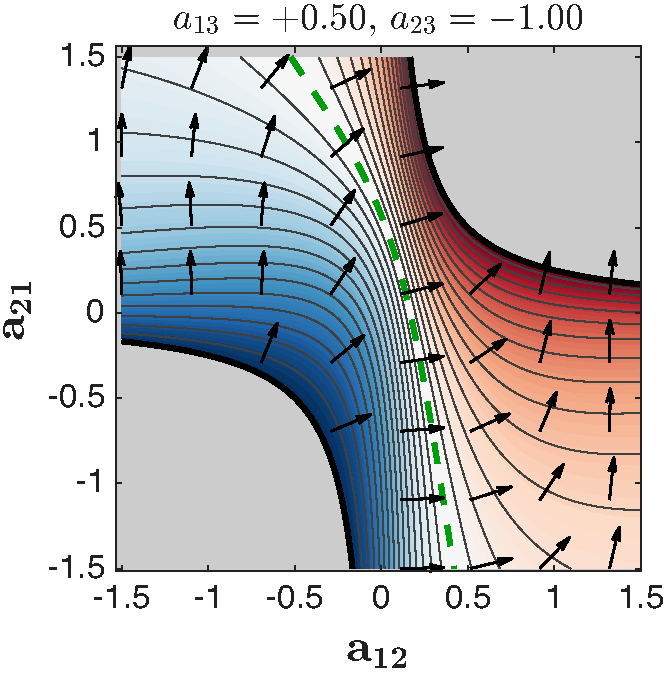
\includegraphics[width=\linewidth]{figures/topo_3node_moderator_figures/C2.pdf}};
\node[overlay,anchor=south west,font=\bfseries\footnotesize,xshift=\labxshiftB,yshift=0.58pt] at (imgB2.south west) {C2};
\end{tikzpicture}
\end{minipage}
&
\begin{minipage}[b]{\cellwd}
\centering
\begin{tikzpicture}[inner sep=0pt,outer sep=0pt]
\node[inner sep=0pt] (imgB3) {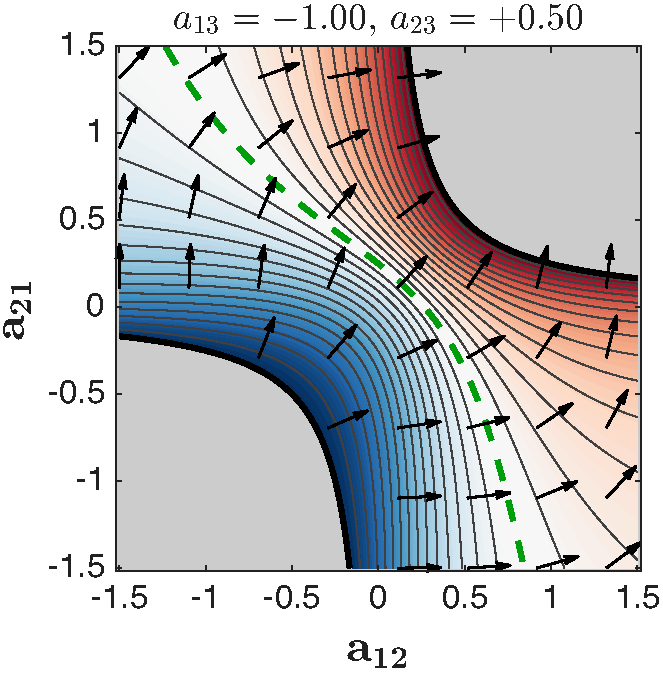
\includegraphics[width=\linewidth]{figures/topo_3node_moderator_figures/C3.pdf}};
\node[overlay,anchor=south west,font=\bfseries\footnotesize,xshift=\labxshiftB,yshift=0.58pt] at (imgB3.south west) {C3};
\end{tikzpicture}
\end{minipage}
\end{tabular}

\vspace{6pt}\hrule height 0.6pt\vspace{6pt}\nointerlineskip   % Divider 3
% --- colorbar (spans \rowwd) ---
\includegraphics[width=\rowwd]{figures/topo_3node_moderator_figures/colorbar.pdf}
\par
\vspace{3pt}
\end{minipage}%
}}
\end{figure}

% caption OUTSIDE the float; \addtocounter rolls back the phantomsubcaption bump
\addtocounter{figure}{-1}
\captionof{figure}{Moderator network.
Each panel is a contour/vector field plot of equation~(\ref{eq:rho21_moderator_main}) for
$\rho_{21}$ as a function of $a_{12}$ and $a_{21}$, over
$a_{12},a_{21}\in[-1.5,1.5]$, across six combinations of $a_{13}$ and
$a_{23}$ (node~3's driving connections, shown in each panel's title), with
$a_{13},a_{23}\in[-1,1]$ and $a=-0.5$ fixed throughout.
$\sigma_{W_1}=\sigma_{W_3}=1$ throughout; $\sigma_{W_2}=1$ for row~B
(panels~\hyperref[fig:moderator_B1]{B1}--\hyperref[fig:moderator_B3]{B3})
and $\sigma_{W_2}=3$ for row~C
(panels~\hyperref[fig:moderator_C1]{C1}--\hyperref[fig:moderator_C3]{C3}).
Panel~\hyperref[fig:moderator_B1]{B1} ($a_{13}=a_{23}=0$) recovers the
dyadic formula~(\ref{eq:rho21_dyad}) exactly; the remaining five panels
(\hyperref[fig:moderator_B2]{B2}--\hyperref[fig:moderator_C3]{C3}) vary
both the magnitude and sign of $a_{13}$ and $a_{23}$, showing that the
driving connections' \emph{direction} and \emph{magnitude} reshape the
correlation surface.
Color encodes $\rho_{21}$ on a diverging scale from $-1$ (blue) through white
to $+1$ (red); values with $|\rho_{21}|<0.05$ are shown in white.
The dashed green curve marks $\rho_{21}=0$ exactly.
The solid black curve is the Hurwitz stability boundary $a_{12}a_{21}=a^2$,
unaffected by $a_{13}$ or $a_{23}$ since node~3 does not feed back into
nodes~1 or~2; the grey region outside it is where no steady state exists
and $\rho_{21}$ is undefined.}
\label{fig:rho21_moderator}

% ============================================================
\subsection*{Coupled Drivers}
% ============================================================

The coupled-drivers network
(Figure~\ref{fig:sigma33_coupled}\hyperref[fig:coupled_A1]{.A1})
combines reciprocal dyadic interaction between nodes~1
and~2 ($a_{12}\neq0$, $a_{21}\neq0$) with unidirectional
connections from both nodes to a downstream node~3
($a_{31}\neq0$, $a_{32}\neq0$). Because $\mathbf{A}$ is block lower triangular, with the
dyadic $2\times2$ block in its upper-left corner and the
scalar $a$ in its lower-right, its eigenvalues are exactly
those of the dyad together with $a$ itself. Hurwitz stability
therefore reduces to the same condition as the dyad, $a<0$
and $a_{12}a_{21}<a^2$.
Solving the Lyapunov equation for this coupled drivers
network confirms that the entries $\sigma_{21}$,
$\sigma_{11}$, and $\sigma_{22}$ of the steady-state
covariance matrix are independent of $a_{31}$ and $a_{32}$,
% Headline result: coupled-drivers rho_21 -- coincides exactly with the
% dyadic formula (eq:rho21_dyad) at a11=a22=a; derived in Appendix D.
yielding (\hyperref[app:appD]{Appendix~D},
equation~\ref{eq:rho21_coupled})
\begin{equation}
\rho_{21} = \frac{|a|\bigl(a_{21}\sigma_{W_1}+a_{12}\sigma_{W_2}\bigr)}
                 {\sqrt{D_{11}\,D_{22}}},
\label{eq:rho21_coupled_main}
\end{equation}
where
\begin{align}
D_{11} &= \bigl(2a^2-a_{12}a_{21}\bigr)\sigma_{W_1}
          + a_{12}^2\,\sigma_{W_2},
\label{eq:D11_coupled_main}\\
D_{22} &= \bigl(2a^2-a_{12}a_{21}\bigr)\sigma_{W_2}
          + a_{21}^2\,\sigma_{W_1}.
\label{eq:D22_coupled_main}
\end{align}
Equation~(\ref{eq:rho21_coupled_main}) coincides exactly with the dyadic
formula~(\ref{eq:rho21_dyad}) evaluated at
$a_{11}=a_{22}=a$. Node~3 contributes to the correlations
$\rho_{31}$ and $\rho_{32}$, but it leaves the correlation
between node~1 and node~2 unaltered.
Because $\rho_{21}$ for this topology is identical to
the dyadic case already shown in Figure~\ref{fig:rho21_dyad}, the
quantity illustrated below is instead the steady-state
\emph{variance} of the receiving node, $\sigma_{33}$, which does
% Headline result: coupled-drivers plots sigma_33, not rho_21, since rho_21
% here is identical to the dyad case already shown; sigma_33 is the
% quantity that actually depends on a31/a32. Derived in Appendix D.
depend on $a_{31}$ and $a_{32}$ (\hyperref[app:appD]{Appendix~D},
equation~\ref{eq:sigma33_coupled}):
\begin{equation}
\sigma_{33} = -\frac{1}{|\mathbf{K}|}\Bigl\{
  E_{1}\,\sigma_{W_1} + E_{2}\,\sigma_{W_2} + E_{3}\,\sigma_{W_3}
\Bigr\},
\label{eq:sigma33_coupled_main}
\end{equation}
where
\begin{align}
E_{1} &= 16a^3a_{31}^2 - 24a^2a_{21}a_{31}a_{32}
        + 12aa_{21}^2a_{32}^2 - 4aa_{12}a_{21}a_{31}^2,
\label{eq:E1_coupled}\\
E_{2} &= 16a^3a_{32}^2 - 24a^2a_{12}a_{31}a_{32}
        + 12aa_{12}^2a_{31}^2 - 4aa_{12}a_{21}a_{32}^2,
\label{eq:E2_coupled}\\
E_{3} &= 32a^5 - 40a^3a_{12}a_{21} + 8aa_{12}^2a_{21}^2.
\label{eq:E3_coupled}
\end{align}
Unlike every correlation $\rho_{ij}$ considered elsewhere in this
paper, $\sigma_{33}$ is not bounded to $[-1,1]$. Instead, it is always non-negative and unbounded from above as $a_{31}$ and
$a_{32}$ increase.
The connections $a_{31}$ and $a_{32}$ enter only through $E_1$
and $E_2$, which are independent of $\sigma_{W_3}$; the node's
own noise variance $\sigma_{W_3}$ enters only through $E_3$,
which is independent of $a_{31}$ and $a_{32}$.
Because $\sigma_{33}$ depends on $a_{31}$ and $a_{32}$ only
through $a_{31}^2$, $a_{32}^2$, and the cross term
$a_{31}a_{32}$, it is invariant under
$(a_{31},a_{32})\to(-a_{31},-a_{32})$, and reversing just one
of the two rotates the surface by $180^\circ$ rather than
reshaping it.
The coefficient of $\sigma_{W_3}$, $E_3/|\mathbf{K}|$, reduces
exactly to $1/(2|a|)$, independent of every causal parameter,
so $\sigma_{W_3}$ shifts $\sigma_{33}$ by a constant everywhere
on the plane rather than reshaping its dependence on $a_{31}$
and $a_{32}$.
At $a_{12}=a_{21}=0$, this closed form reduces to
$\sigma_{33}=\bigl(a_{31}^2\sigma_{W_1}+a_{32}^2\sigma_{W_2}\bigr)/(4|a|^3)
+\sigma_{W_3}/(2|a|)$, the independent-node floor plus the
variance injected by the two drivers.

% ============================================================
% Coupled drivers figure -- individual-panel template (produced per
% tasks/stage3_tasks_plot_networks/stage3_topo_x-node_figure_template_instructions.md).
% Panels exported by
% scripts/plot_networks/plot_topo_3node_coupled_drivers_subplot.m to
% figures/topo_3node_coupled_drivers_figures/. Plots sigma_33 (variance),
% not rho_21 -- see prose above. Sequential (viridis-like) LOG-scale
% colormap, not the diverging rho colormap: see the script header for the
% full rationale (no zero-crossing, no stability mask needed since a31/a32
% do not affect stability, log scale chosen since floor-to-ceiling spans
% ~1.5 log10-decades). Two subplot rows (A/B); no row C.
% ============================================================
\begin{figure}[H]
\centering
{\setlength{\fboxrule}{0.6pt}\setlength{\arrayrulewidth}{0.6pt}%
\fbox{%
\begin{minipage}{\dimexpr\textwidth-2\fboxsep-2\fboxrule\relax}
\centering
\setlength{\cellwd}{\dimexpr(0.95\linewidth-12pt)/3\relax}
\setlength{\rowwd}{\dimexpr3\cellwd+12pt\relax}
\setlength{\labxshiftB}{-0.26pt}
\vspace{3pt}
% --- title ---
{\normalsize\textbf{$\sigma_{33}$ as a function of $a_{12}$ and $a_{21}$ (coupled drivers)}}\par
\vspace{6pt}\hrule height 0.6pt\vspace{6pt}\nointerlineskip   % Divider 4
% --- structure strip: diagram | A | Sigma_W ---
% --- structure strip labels A1-A3 -- see dyad figure's comment
% for the label mechanism.
\renewcommand{\thesubfigure}{A1}
\phantomsubcaption\label{fig:coupled_A1}
\renewcommand{\thesubfigure}{A2}
\phantomsubcaption\label{fig:coupled_A2}
\renewcommand{\thesubfigure}{A3}
\phantomsubcaption\label{fig:coupled_A3}
\begin{tabular}{c@{\hspace{6pt}}|@{\hspace{6pt}}c@{\hspace{6pt}}|@{\hspace{6pt}}c}
\begin{minipage}[c]{\cellwd}
\centering
\def\a{1.0 cm}
\def\nodeSize{0.7}
\def\r{0.5*\nodeSize cm}
\begin{tikzpicture}[inner sep=0pt,outer sep=0pt]
\node[inner sep=0pt] (coupledDiagram) {%
\begin{tikzpicture}[
    >={Stealth[length=3mm,width=2mm]},
    every node/.style={circle,draw,
        minimum size=\nodeSize cm}]
\node (1) at (-\a,0)          {1};
\node (2) at (\a,0)           {2};
\node (3) at (0,{sqrt(3)*\a}) {3};
\draw[->] (1) to[bend left=12]  (2);
\draw[->] (2) to[bend left=12]  (1);
\draw[->] (1) to[bend left=12]  (3);
\draw[->] (2) to[bend right=12] (3);
\selfloop{1}{1}
\selfloop{2}{2}
\selfloop{3}{3}
\end{tikzpicture}%
};
\useasboundingbox (-0.5\cellwd,-45.35pt) rectangle (0.5\cellwd,45.35pt);
\node[overlay,anchor=south west,font=\bfseries\footnotesize,xshift=-3.26pt,yshift=3.91pt] at (current bounding box.south west) {A1};
\end{tikzpicture}
\end{minipage}
&
\begin{minipage}[c]{\cellwd}
\centering
\begin{tikzpicture}[inner sep=0pt,outer sep=0pt]
\node[inner sep=0pt] (matA) {$\mathbf{A}=\begin{bmatrix}
a      & a_{12} & 0\\
a_{21} & a      & 0\\
a_{31} & a_{32} & a
\end{bmatrix}$};
\useasboundingbox (-0.5\cellwd,-45.35pt) rectangle (0.5\cellwd,45.35pt);
\node[overlay,anchor=south west,font=\bfseries\footnotesize,xshift=\labxshiftB,yshift=3.91pt] at (current bounding box.south west) {A2};
\end{tikzpicture}
\end{minipage}
&
\begin{minipage}[c]{\cellwd}
\centering
\begin{tikzpicture}[inner sep=0pt,outer sep=0pt]
\node[inner sep=0pt] (matSW) {$\mathbf{\Sigma}_W=\begin{bmatrix}
\sigma_{W_1}&0&0\\0&\sigma_{W_2}&0\\0&0&\sigma_{W_3}
\end{bmatrix}$};
\useasboundingbox (-0.5\cellwd,-45.35pt) rectangle (0.5\cellwd,45.35pt);
\node[overlay,anchor=south west,font=\bfseries\footnotesize,xshift=\labxshiftB,yshift=3.91pt] at (current bounding box.south west) {A3};
\end{tikzpicture}
\end{minipage}
\end{tabular}
\vspace{6pt}\hrule height 0.6pt\vspace{6pt}\nointerlineskip   % Divider 1
% --- Row A ---
\renewcommand{\thesubfigure}{B1}\phantomsubcaption\label{fig:coupled_B1}
\renewcommand{\thesubfigure}{B2}\phantomsubcaption\label{fig:coupled_B2}
\renewcommand{\thesubfigure}{B3}\phantomsubcaption\label{fig:coupled_B3}
\begin{tabular}{c@{\hspace{6pt}}|@{\hspace{6pt}}c@{\hspace{6pt}}|@{\hspace{6pt}}c}
\begin{minipage}[b]{\cellwd}
\centering
\begin{tikzpicture}[inner sep=0pt,outer sep=0pt]
\node[inner sep=0pt] (imgA1) {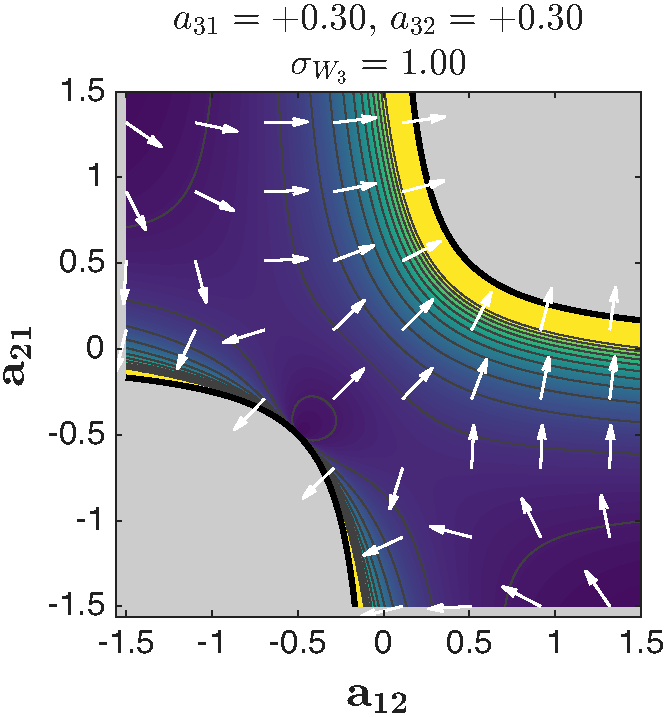
\includegraphics[width=\linewidth]{figures/topo_3node_coupled_drivers_figures/B1.pdf}};
\node[overlay,anchor=south west,font=\bfseries\footnotesize,xshift=-3.26pt,yshift=0.58pt] at (imgA1.south west) {B1};
\end{tikzpicture}
\end{minipage}
&
\begin{minipage}[b]{\cellwd}
\centering
\begin{tikzpicture}[inner sep=0pt,outer sep=0pt]
\node[inner sep=0pt] (imgA2) {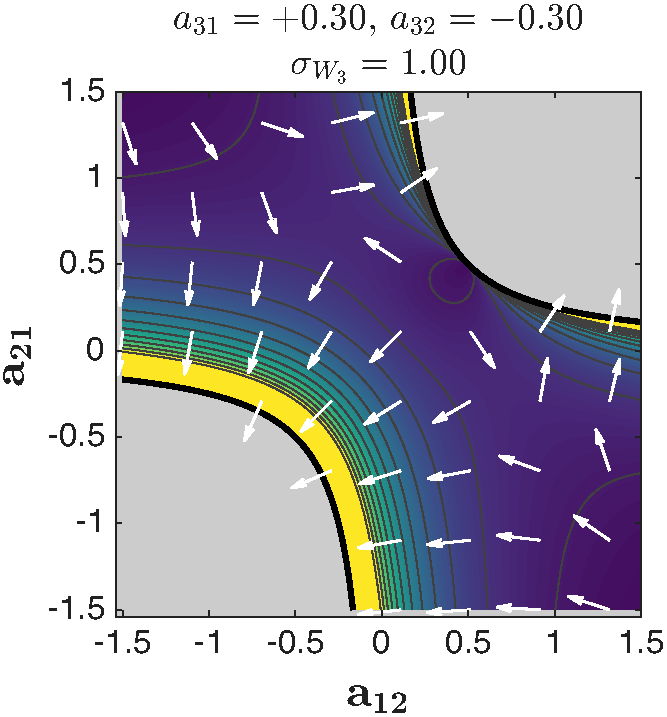
\includegraphics[width=\linewidth]{figures/topo_3node_coupled_drivers_figures/B2.pdf}};
\node[overlay,anchor=south west,font=\bfseries\footnotesize,xshift=\labxshiftB,yshift=0.58pt] at (imgA2.south west) {B2};
\end{tikzpicture}
\end{minipage}
&
\begin{minipage}[b]{\cellwd}
\centering
\begin{tikzpicture}[inner sep=0pt,outer sep=0pt]
\node[inner sep=0pt] (imgA3) {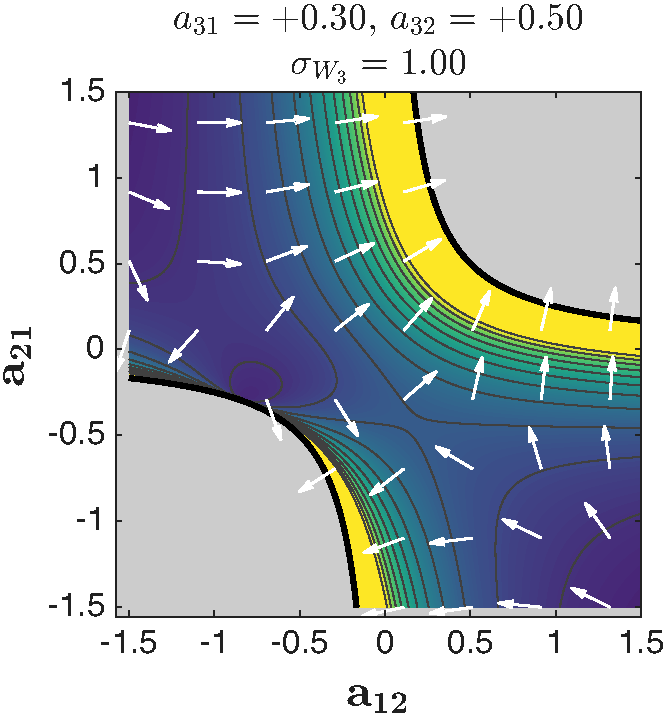
\includegraphics[width=\linewidth]{figures/topo_3node_coupled_drivers_figures/B3.pdf}};
\node[overlay,anchor=south west,font=\bfseries\footnotesize,xshift=\labxshiftB,yshift=0.58pt] at (imgA3.south west) {B3};
\end{tikzpicture}
\end{minipage}
\end{tabular}
\par
\vspace{6pt}\hrule height 0.6pt\vspace{6pt}\nointerlineskip   % Divider 2
% --- Row B ---
\renewcommand{\thesubfigure}{C1}\phantomsubcaption\label{fig:coupled_C1}
\renewcommand{\thesubfigure}{C2}\phantomsubcaption\label{fig:coupled_C2}
\renewcommand{\thesubfigure}{C3}\phantomsubcaption\label{fig:coupled_C3}
\begin{tabular}{c@{\hspace{6pt}}|@{\hspace{6pt}}c@{\hspace{6pt}}|@{\hspace{6pt}}c}
\begin{minipage}[b]{\cellwd}
\centering
\begin{tikzpicture}[inner sep=0pt,outer sep=0pt]
\node[inner sep=0pt] (imgB1) {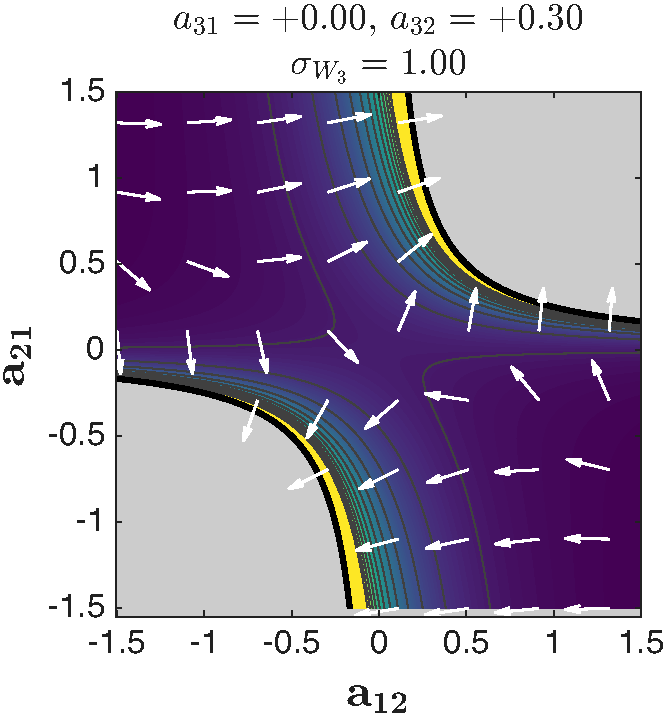
\includegraphics[width=\linewidth]{figures/topo_3node_coupled_drivers_figures/C1.pdf}};
\node[overlay,anchor=south west,font=\bfseries\footnotesize,xshift=-3.26pt,yshift=0.58pt] at (imgB1.south west) {C1};
\end{tikzpicture}
\end{minipage}
&
\begin{minipage}[b]{\cellwd}
\centering
\begin{tikzpicture}[inner sep=0pt,outer sep=0pt]
\node[inner sep=0pt] (imgB2) {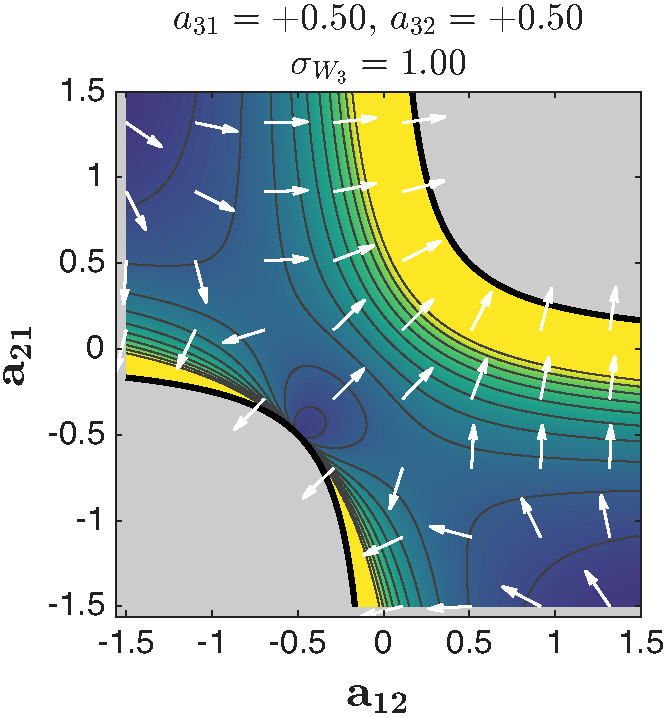
\includegraphics[width=\linewidth]{figures/topo_3node_coupled_drivers_figures/C2.pdf}};
\node[overlay,anchor=south west,font=\bfseries\footnotesize,xshift=\labxshiftB,yshift=0.58pt] at (imgB2.south west) {C2};
\end{tikzpicture}
\end{minipage}
&
\begin{minipage}[b]{\cellwd}
\centering
\begin{tikzpicture}[inner sep=0pt,outer sep=0pt]
\node[inner sep=0pt] (imgB3) {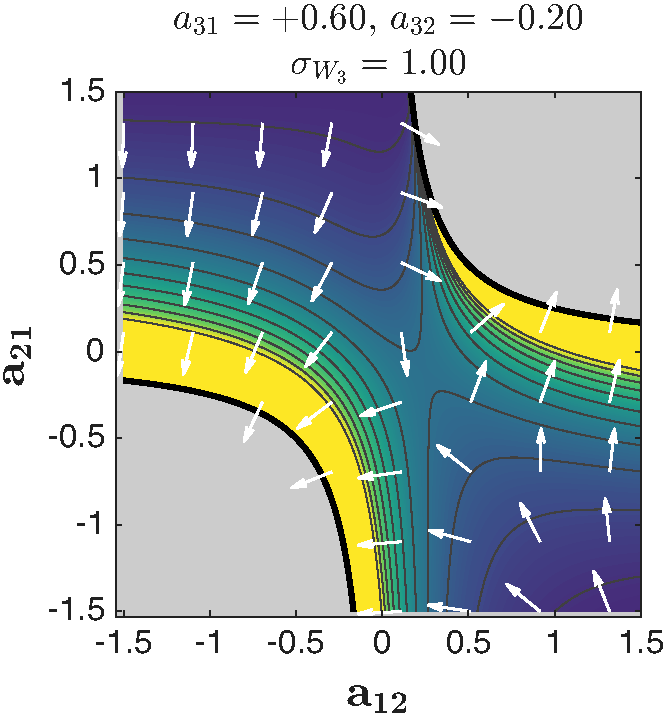
\includegraphics[width=\linewidth]{figures/topo_3node_coupled_drivers_figures/C3.pdf}};
\node[overlay,anchor=south west,font=\bfseries\footnotesize,xshift=\labxshiftB,yshift=0.58pt] at (imgB3.south west) {C3};
\end{tikzpicture}
\end{minipage}
\end{tabular}

\vspace{6pt}\hrule height 0.6pt\vspace{6pt}\nointerlineskip   % Divider 3
% --- colorbar (spans \rowwd) ---
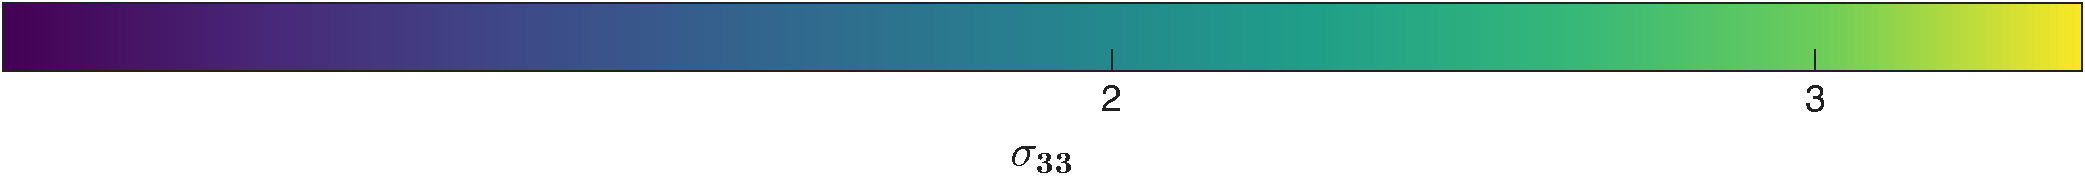
\includegraphics[width=\rowwd]{figures/topo_3node_coupled_drivers_figures/colorbar.pdf}
\par


\vspace{3pt}
\end{minipage}%
}}
\end{figure}

% caption OUTSIDE the float; \addtocounter rolls back the phantomsubcaption bump
\addtocounter{figure}{-1}
\captionof{figure}{Coupled drivers network.
Each panel is a contour/vector field plot of equation~(\ref{eq:sigma33_coupled_main}) for
$\sigma_{33}$ as a function of $a_{12}$ and $a_{21}$ over
$a_{12},a_{21}\in[-1.5,1.5]$, with $a=-0.5$ and
$\sigma_{W_1}=\sigma_{W_2}=\sigma_{W_3}=1$ fixed throughout.
Panels~\hyperref[fig:coupled_B1]{B1}--\hyperref[fig:coupled_C3]{C3} fix
$(a_{31},a_{32})$ at $(+0.30,+0.30)$, $(+0.30,-0.30)$, $(+0.30,+0.50)$,
$(0,+0.30)$, $(+0.50,+0.50)$, and $(+0.60,-0.20)$ respectively, shown in
each panel's title.
Color encodes $\log_{10}\sigma_{33}$ on a sequential scale from dark purple
(low) to yellow (high), capped at $\sigma_{33}=3.5$ (about $10\%$ of the
stable region saturates at the top color); the colorbar is labeled with the
corresponding untransformed $\sigma_{33}$ values.
Arrows show the gradient direction of $\sigma_{33}$.
The solid black curve is the Hurwitz stability boundary $a_{12}a_{21}=a^2$,
with the grey region beyond it --- no steady state, $\sigma_{33}$
undefined.}
\label{fig:sigma33_coupled}

% ============================================================
\subsection*{Fully Connected Three-Node Network}
% ============================================================

Taken together, Figures~\ref{fig:rho21_dyad}--\ref{fig:rho21_moderator} illustrates how the correlation between two variables (nodes) changes with the \emph{presence} or \emph{absence} of a third variable, and with the way the third node interacts with the first two. From the simplest dyad
(Figure~\ref{fig:rho21_dyad}) to the more complex moderator (Figure~\ref{fig:rho21_moderator}) networks, we see how the pairwise
correlation $\rho_{21}$ takes on markedly different ``causal'' geometries. Each of these architectures is a special case of the fully connected triad, which we unpack here.
The fully connected three-node network allows all six
off-diagonal causal connections to be nonzero. The diagonal entries $a_{ii}$ encode self-connections and
are generally unequal to each other. Solving the Lyapunov equation for the general asymmetric
% Headline result: general (dense-A) 3-node sigma_ij and rho_ij, the
% capstone result all eight preceding topologies specialize -- derived in
% Appendix D via lyap_halfvec.m directly (A has no exploitable sparsity).
$3\times3$ network yields closed-form expressions for all
entries of $\mathbf{\Sigma}_Y$,
\begin{equation}
\sigma_{ij} = -\frac{1}{|\mathbf{K}|}
\Bigl[
  f_{ij}^{(i)}(\mathbf{A})\,\sigma_{W_i}
  + f_{ij}^{(j)}(\mathbf{A})\,\sigma_{W_j}
  + f_{ij}^{(k)}(\mathbf{A})\,\sigma_{W_k}
\Bigr],
\quad \{i,j,k\}=\{1,2,3\},
\label{eq:sigma_ij_3x3}
\end{equation}
where $|\mathbf{K}|$ is the determinant of the half-vectorized Kronecker sum
($\mathbf{I}\otimes\mathbf{A}
+\mathbf{A}\otimes\mathbf{I}$) and the polynomial coefficient
functions $f_{ij}^{(\cdot)}(\mathbf{A})$ are given explicitly
in \hyperref[app:appD]{Appendix~D}
(equations~\ref{eq:network3by3_sigma_ii}
and~\ref{eq:network3by3_sigma_ij_v2}).
The pairwise correlation is
\begin{equation}
\rho_{ij} = \frac{\sigma_{ij}}
                 {\sqrt{\sigma_{ii}\,\sigma_{jj}}}.
\label{eq:rho_ij_3x3}
\end{equation}

No contour plots are shown for this topology. With six
independent off-diagonal connections and three unrestricted
diagonal entries, the $\sigma_{ij}$ formula above has
dozens of polynomial terms for each noise variance (\hyperref[app:appD]{Appendix~D}), too
complex to visualize meaningfully in a two-parameter plane. However, several properties of the
formulas~(\ref{eq:sigma_ij_3x3}) are noteworthy.

\vspace{6pt}
\textit{Structural and reflective symmetry.}
The fully connected topology is invariant under swapping the
labels of the two non-focal nodes ($j \leftrightarrow k$ for
fixed $i$), and the variance formulae $\sigma_{ii}$ inherit
this invariance. The covariance formulas $\sigma_{ij}$ are invariant under $i \leftrightarrow j$ for fixed $k$,
reflecting the symmetry $\sigma_{ij}=\sigma_{ji}$ of the
covariance matrix itself.
Neither invariance is immediately obvious from the raw
polynomial coefficients, but both become visually apparent in
the color-coded templates of
\hyperref[app:appD]{Appendix~D}
(equations~\ref{eq:network3by3_sigma_ii}
and~\ref{eq:network3by3_sigma_ij_v2}), and each provides a
consistency check on the derivation.

\vspace{6pt}
\textit{The ``master formula'' for $3\times3$ networks.}
The covariance formula for every sparse three-node topology is a special case of
equation~(\ref{eq:sigma_ij_3x3}), recovered by setting the
appropriate entries of $\mathbf{A}$ to zero:
\begin{itemize}
\item confounder: set $a_{12}=a_{21}=a_{31}=a_{32}=0$;
\item mediator: set $a_{12}=a_{21}=a_{13}=a_{32}=0$;
\item moderator: set $a_{31}=a_{32}=0$.
\end{itemize}
Reduction to the formulae for the confounder network was verified through
direct symbolic elimination, recovering the
independently derived covariance
formulae~(\ref{eq:sigma11_confounder})--(\ref{eq:sigma32_confounder})
and determinant~(\ref{eq:network3by3_detK_confounder}) exactly.
The fully connected $3\times3$ formula thus serves as
\textit{the ``master formula'' for $3\times3$ networks}.

% ============================================================
% ============================================================
%  DISCUSSION
% ============================================================
% ============================================================
%  DISCUSSION SECTION
%  For: "How does correlation relate to causation"
%  Author: Yaohui Ding
% ============================================================

\section*{Discussion}

% ------------------------------------------------------------
\subsection*{Correlation Is Symmetric but Not Transitive}
% ------------------------------------------------------------

Correlation is symmetric by definition, $\rho_{ij}=\rho_{ji}$. However, it is \emph{not} transitive. A mathematical relation ($\sim$) is transitive, if $x\sim y$
and $y\sim z$ together imply $x\sim z$. For example, ``is a cousin of'' is not a transitive relation. A is a cousin of B (premise no. 1) and B is a cousin of C (premise no. 2) together do not imply A is a cousin of C (conclusion), necessarily. The premises would still be true if A and C were siblings and B was their cousin. However, the conclusion would be wrong in this case. 
The collider topology in the results section provides a simple and intuitive example of the fact that correlation is not a transitive relation, either. In this network topology, $\rho_{31}$ and
$\rho_{32}$ are both nonzero (sometimes fairly strong, Figure~\ref{fig:rho31_collider}\hyperref[fig:collider_B1]{.B1}) whenever $a_{31}\neq0$ and
$a_{32}\neq0$~(Equation (\ref{eq:rho31_collider_main})), yet
$\rho_{21}$ is always 0 by construction~(Equation (\ref{eq:rho21_collider})).
Thus, node~1 correlating with node~3 ($\rho_{13}=\rho_{31}\neq0$) and node~3 correlating with node~2 ($\rho_{32}\neq0$) does not lead to node~1 correlating with node~2 ($\rho_{12}=\rho_{21}=0$). Correlation is \emph{not} transitive. For a more thorough treatment of the \emph{non-transitivity} of correlation, see \citet{LangfordSchwertmanOwens2001}. In this paper, they prove that $\rho_{XZ}$ must be
positive ($>0$) whenever $\rho_{XY}^2+\rho_{YZ}^2>1$. The result ($\rho_{21}=0$) from our collider network offers an example of what might happen when this sum of squared correlation coefficients constraint is violated. In our setting, we have
\begin{equation*}
\rho_{31}^2+\rho_{32}^2 = \frac{a_{31}^2\sigma_{W_1}+a_{32}^2\sigma_{W_2}}
{2\bigl(2a^2\sigma_{W_3}+a_{31}^2\sigma_{W_1}+a_{32}^2\sigma_{W_2}\bigr)}
< \frac{1}{2}
\end{equation*}
because $\sigma_{W_3}$ is always greater than zero ($>0$) and $a\neq0$. But $\rho_{21}$ equals 0, not greater than 0. This raises an interesting possibility that there may exist a different bound for $\rho_{XZ}$, when $\rho_{XY}^2+\rho_{YZ}^2\leq1$.


% ------------------------------------------------------------
\subsection*{Causation Is Transitive: From Tracing Rule to
             Trek Rule}
% ------------------------------------------------------------

Causal influence is, in general, \emph{asymmetric}.
However, it is \emph{transitive}. The formula from the mediator network (equation~\ref{eq:rho21_mediator_main}) illustrates this transitivity of causation intuitively. Node~1
reaches node~2 through the chain $1\to3\to2$.
The resulting correlation (composite causal influence) is therefore proportional to the
product of $a_{31}a_{23}$ and \emph{never} 0, unless $a_{31}$ or $a_{23}$ or both are zero. Wright proved this over a century ago for models that can be represented by directed acyclic graphs \citep{Wright1921}. He showed that the correlation (composite causal effect) between any pair of variables is the sum, over every connecting path, of the
products of the path coefficients along it. Crucially, the composite causal effect (transitivity of causation) along a given path is \emph{never} zero, provided that the causal influence of every link in the path is non-zero. \citet{VarandoHansen2020} and \citet{HansenTrek2025} generalized the transitivity of causal influence to cyclic graphs with feedback. They showed that each covariance $\sigma_{ij}$ is an infinite power series over ``treks'' --- the same
compositional idea, now summed over infinitely many paths.
The closed-form formula that we derive in
\hyperref[app:appB]{Appendix~B} (equation~\ref{eq:sigma_ij_final}) can be read
as the exact summation of these infinite power series. The cofactor
representation collapses infinitely many treks into a finite
ratio of polynomials. 


% ------------------------------------------------------------
\subsection*{Many-to-One Mapping from Patterns of Causation
             to Correlation}
% ------------------------------------------------------------

When $\mathbf{A}$ is Hurwitz stable,
the Lyapunov equation~(\ref{eq:lyapunov_eq0}) has a unique
solution $\mathbf{\Sigma}_Y$ for any given pair of
$\mathbf{A}$ and $\mathbf{\Sigma}_W$
\citep{Antsaklis1997, Hespanha2018}. Therefore, a given causal architecture
and noise covariance jointly determine exactly one pattern
of correlations. However, the reverse is not true. The same pattern of correlation can correspond to many distinct causal architectures and noise covariance structures (\emph{one-to-many}). The Results section provides many concrete examples. An identical value of $\rho_{21}$ can arise from direct
reciprocal coupling between node~1 and node~2 with no hidden
variables~(\ref{eq:rho21_dyad}) or entirely from a common cause with no direct causal interaction between them~(\ref{eq:rho21_confounder}). More strikingly, the collider maps every combination of $a_{31}$, $a_{32}$ to the same vanishing
correlation of $\rho_{21}=0$~(\ref{eq:rho21_collider}).

This under-determination problem of inferring causes from effects (e.g., patterns of correlation) is well recognized in the causal
inference literature \citep{Pearl2009, PetersJanzingScholkopf2017,
SpirtesGlymourScheines2000}. Identifiability of causal networks with
structural constraints remains an active research area
\citep{VarandoHansen2020, DettlingEtAl2023}.


% ------------------------------------------------------------
\subsection*{Linear in Noise Variances but Nonlinear in Causal Parameters}
% ------------------------------------------------------------

The general solution of the covariance matrix from the Lyapunov equation
(Methods, equation~\ref{eq:sigma_ij_general};
\hyperref[app:appB]{Appendix~B}, equation~\ref{eq:sigma_ij_final})
exhibits a structural duality. Each entry
$\sigma_{ij}$ is a \textit{linear combination} of the noise
variances $\sigma_{W_u}$, with weights that are
\textit{nonlinear} (polynomial) functions of the causal
parameters $a_{ij}$.
The linearity of the noise variances follows directly from the structure of
the solution---
noise variance enters the equation through the sum
$\sum_{u} C_{ij}^{uu}\,\sigma_{W_u}$. The cofactor matrix entry $C_{ij}^{uu}$ and the
determinant $|\mathbf{K}|$ depend only on $\mathbf{A}$. However, the
nonlinearity of $C_{ij}^{uu}$ and $|\mathbf{K}|$ in the entries of matrix $\mathbf{A}$ grow quickly with network size.
The covariance formulae for the dyadic network have only second-degree
coefficients~(\ref{eq:rho21_dyad}), whereas the formulae from triadic networks carry fifth-degree coefficients
(\hyperref[app:appD]{Appendix~D}, equation~\ref{eq:sigma33_coupled}). This linear-in-noise property is specific to the covariance, however
(Results, equation~\ref{eq:rho_ij_general}
\hyperref[app:appB]{Appendix~B}, equation~\ref{eq:rho_ij_nbyn}),
because $\rho_{ij}=\sigma_{ij}/\sqrt{\sigma_{ii}\,\sigma_{jj}}$
places the variance terms under a square root. The noise
variances enter $\rho_{ij}$ nonlinearly, even though
$\sigma_{ij}$, $\sigma_{ii}$, and $\sigma_{jj}$ are each
individually linear in them.


% ------------------------------------------------------------
\subsection*{Structural Symmetry and Reducibility of the
             ``Master Formulae'' from Fully Connected $N\times N$
             Network}
% ------------------------------------------------------------

The formula for $\sigma_{ii}$ from the fully-connected $3\times3$ network shows \textit{structural symmetry} (\hyperref[app:appD]{Appendix~D}, equation~\ref{eq:network3by3_sigma_ii}), because the network's topology is invariant under the relabeling ($j\leftrightarrow k$) for fixed $i$. We emphasize that this symmetry is a property of the topology of the fully-connected $3\times3$ network itself (hence structural), not a property of the formula for $\sigma_{ii}$ in
general. In contrast, the formulae for the covariance entry $\sigma_{ij}$ (when $i \neq j$) have to satisfy 
\textit{reflective symmetry} (\hyperref[app:appD]{Appendix~D}, equation~\ref{eq:network3by3_sigma_ij_v2}), i.e., invariant under
$i\leftrightarrow j$ for fixed $k$, for all types of network topologies. We made both types of symmetries for the fully-connected $3\times3$ network visually apparent in \hyperref[app:appD]{Appendix~D}, by color-coding the indices ($i,j,k$) and re-arranging the terms in a specific way. The formulae from the fully connected $3\times3$ network can also serve as the ``\textit{master
formulae}'' for deriving the formulae for every other $3\times3$ network with a sparser topology, by setting the
appropriate causal connections in the ``master formulae'' to zero, provided that Hurwitz stability condition is still satisfied. We verified this for the confounder network in \hyperref[app:appD]{Appendix~D} (equations~\ref{eq:sigma11_confounder}--\ref{eq:sigma32_confounder}
and~\ref{eq:network3by3_detK_confounder}). Finally, both the structural symmetry and reducibility properties generalize beyond the $3\times3$ case to the $N\times N$ network with structural symmetry (both the incoming and out-going causal connections exist for any given pairs of nodes). This is because, for $\mathbf{A}$ matrix that has structural symmetry, the Kronecker sum ($(\mathbf{I}\otimes\mathbf{A}+\mathbf{A}\otimes\mathbf{I})$) is also symmetric; hence its inverse is symmetric as well. With diagonal noise covariance constraint, the general solution for $\sigma_{ij}$ shows structural symmetry. 

% ------------------------------------------------------------
\subsection*{Combinatoric Complexity of Determining Correlation
             from Causation}
% ------------------------------------------------------------
The complexity of the closed-form solution for $\sigma_{ij}$
(equation~\ref{eq:sigma_ij_general}) grows rapidly with network size and
connectivity. For the fully connected $ N \times N $ network, the total number of terms in
$\sigma_{ij}$'s numerator grows from 2 for the dyad~(equation \ref{eq:rho21_dyad}), to 55 for the $3\times3$ network
(\hyperref[app:appD]{Appendix~D}, equation~\ref{eq:network3by3_sigma_ij_v2}),
to 9{,}188 for the $4\times4$ network, which we confirmed by symbolically solving for the fully-connected $4\times4$ network. The degree of each term in the numerator of $\sigma_{ij}$ is exactly
$m-1=N(N+1)/2-1$, because every entry of the Kronecker-sum matrix
$\mathbf{K}$ is linear in $\mathbf{A}$. The degree is 2 for the dyad, 5 for the fully connected $3\times3$, and 9
for the fully connected $4\times4$. 
The number of terms, however, grows far faster than the degree ---
nearly two orders of magnitude from $N=3$ to $N=4$. Despite the combinatoric complexity for large N, the entry-level formulae for small networks ($N \le 3$) are tractable and revealing. They make intuitive the ``causal geometries" of pairwise correlation and its noise variance dependence that the full formula obscures. 

% ------------------------------------------------------------
\subsection*{Lyapunov Equation as a Unifying Mathematical Object
             for Causal Modeling of Dynamical Systems with Additive
             White Noise}
% ------------------------------------------------------------

The Lyapunov equation is the common mathematical substrate
of two causal modeling traditions that developed largely
in parallel, namely, Granger causality \citep{Granger1969, BarnettSeth2014} and dynamic causal modeling
\citep{FristonHarrisonPenny2003, DaunizeauStephanFriston2012}. In the Granger-causality tradition, the steady-state autocovariance of the
underlying vector autoregressive model satisfies the \emph{discrete-time}
 Lyapunov equation \citep{Stein1952}. In (spectral) dynamic causal modeling, it links the resting state effective
connectivity matrix $\mathbf{A}$ to the resting state functional connectivity matrix
$\mathbf{\Sigma}_Y$ \citep{Friston2014}, under the symmetric constraint ($\mathbf{A}=\mathbf{A}^T$).


% ------------------------------------------------------------
\subsection*{Limitations of the Mathematical Modeling Framework in the Current Study}
% ------------------------------------------------------------

\textit{Linearity.}
The linear stochastic dynamical
system is among the simplest possible
stochastic models, and many systems of scientific interest
are substantially nonlinear.
In nonlinear systems, the Lyapunov
equation no longer governs the
steady-state covariance, and closed-form expressions of the
type derived here are generally unavailable.
Local linearization around a stable fixed point offers one
extension to weakly nonlinear systems \citep{Gardiner2004},
but its validity depends on the amplitude of fluctuations
relative to the nonlinear terms.

\medskip
\textit{White noise.}
The additive white noise assumption --- uncorrelated across
time --- is what makes the system Markovian
\citep{Gardiner2004}, such that
$\mathbf{\Sigma}_Y$ satisfies the Lyapunov equation. Colored (temporally autocorrelated) noise would break this Markov property and require augmenting the state with
the noise process itself before a Lyapunov-style steady-state
equation could be obtained.

\medskip
\textit{No exogenous input.}
The linear stochastic dynamical systems in our current study do not have time-varying exogenous input. However, many dynamical systems of interest are shaped by external inputs ---
stimuli, treatments, or other interventions. Incorporating them would require augmenting the model with an explicit input term, as in Friston's dynamic causal modeling
framework, whose bilinear state equation includes both exogenous
driving and modulatory inputs \citep{FristonHarrisonPenny2003}.
Pearl's do-calculus \citep{Pearl2009} provides a general
framework for reasoning about the causal effect of
interventions in structural causal models.

\medskip
\textit{Forward vs.\ inverse problem.}
This paper addresses the forward problem: given a particular causal architecture and noise covariance, derive the pattern of correlation that arises at the steady state.
The closed-form expressions may nonetheless be useful for
the inverse problem --- inferring or estimating the underlying causal architecture from the data
--- for instance, by providing analytic gradients for
optimization-based inference, or by characterizing the
identifiable combinations of causal parameters that can be
recovered from observed covariance data alone
\citep{VarandoHansen2020, BongersBlomMooij2022}.


\section*{Code Availability}
No experimental or simulated datasets are analyzed in the current study. All code necessary to reproduce the manuscript is publicly available at \url{https://github.com/yaohuiding1/corr_causation}.

\section*{Acknowledgments}
The author would like to thank John J.B. Allen, Jessica Andrews-Hanna, and Ying-hui Chou for inspiring his curiosity and interest in the topic of causal inference in the begining, in the context of studying how different brain regions causally influence each other at rest. The author would like to thank John Pearson for his comments and feedback on various drafts of the current manuscript. Finally, the author would like to thank Kevin Kuper, Miles Martinez, and Siyu Wang for their helpful discussions on the topic of causal modeling of dynamical systems in general. 

\clearpage
\bibliographystyle{apacite}
\bibliography{corr_causation}

\newpage
\section*{Appendices}

% Each appendix file ends with its own \bibliographystyle{apacite} and
% \bibliography{appendix_X} commands (needed so it can also compile
% standalone). Redirect those two commands here so that, when \input
% into the main manuscript, they populate a LOCAL bibunit bibliography
% (headed "References", same as the main text) instead of the main
% manuscript's global one -- avoiding both the "multiply defined
% citation" warnings and four unwanted extra copies of the full
% reference list.
\let\appendixbibliographystyle\bibliographystyle
\let\appendixbibliography\bibliography
\renewcommand{\bibliographystyle}[1]{}
\renewcommand{\bibliography}[1]{\putbib[#1]}

% apacite's thebibliography environment resets to \bibliographytypesize
% (\normalsize by default) regardless of the surrounding font size, so
% the \footnotesize below would otherwise stop at the "References"
% heading -- redirect it to \footnotesize too, so each appendix's
% reference list matches its own standalone 10pt rendering as well.
\let\appendixbibliographytypesize\bibliographytypesize
\let\bibliographytypesize\footnotesize

% Each appendix's own standalone file is \documentclass{article} (10pt
% default), while this manuscript is 12pt -- \footnotesize in a 12pt
% document is exactly 10pt, so this reproduces each appendix's verified
% standalone layout (no equation re-wrapping needed) instead of letting
% dense equations overflow at the main text's larger 12pt size.
\begin{bibunit}[apacite]
\footnotesize
\documentclass{article}

\usepackage[letterpaper,top=2cm,bottom=2cm,left=2.54cm,right=2.54cm,marginparwidth=1.75cm]{geometry}
\usepackage{amsmath}
\usepackage{amssymb}
\usepackage{xcolor}
\usepackage[normalem]{ulem}
\usepackage[colorlinks=true, allcolors=blue]{hyperref}
\usepackage{comment}
\usepackage[natbibapa]{apacite}

\setlength{\parindent}{0pt}

% =====================================================================
% EDITED COPY of appendix_a_lyapunov_derivation.tex
% All inline reviewer comments and the "Reviewer's Summary" have been removed
% for readability; the reviewer-recommended corrections and citations have
% been incorporated into the text.
% =====================================================================

%\title{Appendix A: Deriving the Lyapunov Equation for Linear Stochastic Dynamical Systems}

%\author{Yaohui Ding}

\begin{document}

%\maketitle

\section*{Appendix A: Deriving the Lyapunov Equation for Linear Stochastic Dynamical Systems}
\phantomsection\label{app:appA}
\renewcommand{\theequation}{A-\arabic{equation}}
\setcounter{equation}{0}

\subsection*{Linear Stochastic Dynamical Systems}
%
% Governing SDE for the system -- everything below derives from this.
The state equation of a linear stochastic dynamical system is often given by
\begin{equation}
d \mathbf{X}(t) = \mathbf{A} \mathbf{X}(t)\, dt + \boldsymbol{\xi} \, d\mathbf{B}_t
\label{eq:lds_state_eq}
\end{equation}

\begin{comment}
With no loss of generality, let us assume $n=d$.
\end{comment}

where $\mathbf{X}(t) \in \mathbb{R}^n,\ \mathbf{B}_t \in \mathbb{R}^d$ and
$\mathbf{A} \in \mathbb{R}^{n \times n} , \boldsymbol{\xi} \in \mathbb{R}^{n \times d}$. We make the following assumptions, which are used throughout the
derivation: (i) $\mathbf{A}$ is Hurwitz (all eigenvalues
have strictly negative real part); (ii) the noise (diffusion) covariance is defined as
$\mathbf{\Sigma}_\mathbf{W}:=\boldsymbol{\xi}\boldsymbol{\xi}^T$, a symmetric
positive-semidefinite matrix that is assumed to be constant and diagonal; (iii) $\mathbf{B}_t$ is a standard $d$-dimensional Brownian motion; and (iv) the initial condition $\mathbf{X}(0)$ is independent of $\mathbf{B}_t$. Equivalently, the noise $\boldsymbol{\xi}\,d\mathbf{B}_t$ has no memory in time: Brownian increments over non-overlapping intervals are independent, so the noise at any two distinct times is uncorrelated, $E[d\mathbf{B}_{\tau_1}\,d\mathbf{B}_{\tau_2}^T]=\mathbf{I}\,\delta(\tau_1-\tau_2)\,d\tau_1\,d\tau_2$. Given this assumption (\citealp[\S1.3]{Pavliotis2014}), we have
%
% Zero mean and covariance Sigma_W dt for the noise increment xi*dB_t --
% used later in the Ito-isometry step.
\begin{equation}
E[\boldsymbol{\xi} d\mathbf{B}_t]=\boldsymbol{\xi} * E[d\mathbf{B}_t]=\boldsymbol{\xi}*\mathbf{0}=\mathbf{0}
\label{eq:noise_mean}
\end{equation}
%
\begin{equation}
Cov(\boldsymbol{\xi} d\mathbf{B}_t)=E[\boldsymbol{\xi} d\mathbf{B}_t d\mathbf{B}^T_t \boldsymbol{\xi}^T]
=\boldsymbol{\xi} E[d\mathbf{B}_t d\mathbf{B}^T_t] \boldsymbol{\xi}^T=
\boldsymbol{\xi} * \mathbf{I}_{d \times d}* \boldsymbol{\xi}^T * dt=\boldsymbol{\xi}\boldsymbol{\xi}^T dt=\mathbf{\Sigma}_\mathbf{W}\, dt
\label{eq:noise_cov}
\end{equation}


%
% seperator %%%%%%%%%%%%%%%%%%%%%%%%%%%%%%%%%%%%%%%%%%%%%%%%%
\subsection*{The Solution $\mathbf{X}(t)$}
% Closed-form (mild) solution of the SDE via variation of parameters:
% deterministic decay of the initial condition, plus a stochastic
% convolution integral over the noise.
The solution to equation~\ref{eq:lds_state_eq}, valid for every $t\ge 0$, is (\citealp[\S3.7]{Pavliotis2014}),
\begin{equation}
\mathbf{X}(t)=e^{\mathbf{A}t}\mathbf{X}(0)+\int_0^t e^{\mathbf{A}(t-\tau)} \boldsymbol{\xi} d\mathbf{B}_\tau
\label{eq:ss_solution}
\end{equation}

% seperator %%%%%%%%%%%%%%%%%%%%%%%%%%%%%%%%%%%%%%%%%%%%%%%%%
Where $\mathbf{X}(0)$ is the initial condition. Let us denote $Cov \left ( \mathbf{X}(0) \right)=\mathbf{\Sigma}_0$. 
\subsection*{Autocovariance of $\mathbf{X}(t)$ }
The autocovariance of the solution $\mathbf{X}(t)$ at two arbitrary time points $t_1$ and $t_2$ is defined as
% seperator %%%%%%%%%%%%%%%%%%%%%%%%%%%%%%%%%%%%%%%%%%%%%%%%%
\begin{equation}
\mathbf{K}_{XX} (t_1, t_2) :=E\Bigl[\Bigl(\mathbf{X}(t_{1})-E\left [\mathbf{X}(t_{1}) \right] \Bigr) \Bigl(\mathbf{X}(t_{2})-E\left [\mathbf{X}(t_{2}) \right] \Bigr)^T \Bigr]
\end{equation}

Without loss of generality, let us assume we are working with mean-centered $\mathbf{X}(t)$. Thus, $E[\mathbf{X}(t_{1})]=E[\mathbf{X}(t_{2})]=\mathbf{0}$, and
\begin{equation}
\begin{aligned}
% Substitute the solution (eq:ss_solution) at both t1,t2 and expand the
% product into 4 cross-terms: IC-IC, noise-noise, and two IC-noise terms.
\mathbf{K}_{XX}(t_1, t_2) &=E\Bigl [\mathbf{X}(t_{1})\mathbf{X}(t_{2})^T \Bigr] \\
&=E\Bigl[\left \{e^{\mathbf{A}t_{1}}\mathbf{X}(0)+\int_0^{t_{1}} e^{\mathbf{A}(t_{1}-\tau_1)} \boldsymbol{\xi} d\mathbf{B}_{\tau_1} \right \} \left \{ e^{\mathbf{A}t_{2}}\mathbf{X}(0)+\int_0^{t_{2}} e^{\mathbf{A}(t_{2}-\tau_2)} \boldsymbol{\xi} d\mathbf{B}_{\tau_2} \right \}^T \Bigr] \\
&= E \left[ e^{\mathbf{A}t_{1}} \mathbf{X}(0) \mathbf{X}(0)^T e^{\mathbf{A}^T t_{2}} \right]  +  E \left [ \left \{ \int_0^{t_{1}} e^{\mathbf{A}(t_{1}-\tau_1)} \boldsymbol{\xi} d\mathbf{B}_{\tau_1} \right \}  \left \{ \int_0^{t_{2}} e^{\mathbf{A}(t_{2}-\tau_2)} \boldsymbol{\xi} d\mathbf{B}_{\tau_2} \right \}^T \right ] +\\
& \quad E \left[ e^{\mathbf{A}t_{1}} \mathbf{X}(0) \left \{ \int_0^{t_{2}} e^{\mathbf{A}(t_{2}-\tau_2)} \boldsymbol{\xi} d\mathbf{B}_{\tau_2} \right \}^T \right] + E \left [ \left \{ \int_0^{t_{1}} e^{\mathbf{A}(t_{1}-\tau_1)} \boldsymbol{\xi} d\mathbf{B}_{\tau_1} \right \} \mathbf{X}(0)^T e^{\mathbf{A}^T t_{2}} \right ]
\end{aligned}
\label{eq:ss_autocov_0}
\end{equation}

% seperator %%%%%%%%%%%%%%%%%%%%%%%%%%%%%%%%%%%%%%%%%%%%%%%%% 1st_term
% Term 1 of the 4-term expansion above (IC-IC): deterministic, factors
% straight out of the expectation.
Let us evaluate the first term on the right hand side of equation \ref{eq:ss_autocov_0}.
\begin{equation}
\begin{aligned}
 E \left[ e^{\mathbf{A}t_{1}} \mathbf{X}(0) \mathbf{X}(0)^T e^{\mathbf{A}^T t_{2}} \right]=
  e^{\mathbf{A}t_{1}}  E\Bigl[\mathbf{X}(0) \mathbf{X}(0)^T \Bigr] e^{\mathbf{A}^T t_{2}} = e^{\mathbf{A}t_{1}} \mathbf{\Sigma}_0 e^{\mathbf{A}^T t_{2}}
\end{aligned}
\label{eq:ss_autocov_1st_term}
\end{equation}

% seperator %%%%%%%%%%%%%%%%%%%%%%%%%%%%%%%%%%%%%%%%%%%%%%%%2nd_term
% Term 3 of the 4-term expansion (IC-noise cross term; label says
% "2nd_term" but this is actually the 3rd of the 4 terms -- term 2, the
% noise-noise term, is deferred to the steady-state-covariance section).
% Vanishes since X(0) and B_t are independent and X(t) is mean-centered.
Now the third term of equation \ref{eq:ss_autocov_0} is,
\begin{equation}
\begin{aligned}
E \left[ e^{\mathbf{A}t_{1}} \mathbf{X}(0) \left \{ \int_0^{t_{2}} e^{\mathbf{A}(t_{2}-\tau_2)} \boldsymbol{\xi} d\mathbf{B}_{\tau_2} \right \}^T \right] &=E\left[ e^{\mathbf{A}t_{1}} \mathbf{X}(0) \right] E \left[ \left \{ \int_0^{t_{2}} e^{\mathbf{A}(t_{2}-\tau_2)} \boldsymbol{\xi} d\mathbf{B}_{\tau_2} \right \}^T \right] \\
& = e^{\mathbf{A}t_{1}} E\left[  \mathbf{X}(0) \right] E \left[ \left \{ \int_0^{t_{2}} e^{\mathbf{A}(t_{2}-\tau_2)} \boldsymbol{\xi} d\mathbf{B}_{\tau_2} \right \}^T \right] \\
&= e^{\mathbf{A}t_{1}} * \mathbf{0} * E \left[ \left \{ \int_0^{t_{2}} e^{\mathbf{A}(t_{2}-\tau_2)} \boldsymbol{\xi} d\mathbf{B}_{\tau_2} \right \}^T \right]=\mathbf{0}
\end{aligned}
\label{eq:ss_autocov_2nd_term}
\end{equation}

Here we utilize the fact that $\mathbf{X}(t)$ is mean-centered and the assumption that the initial condition $\mathbf{X}(0)$ and $\mathbf{B}_t$ are independent from each other.
% Term 4 of the 4-term expansion (noise-IC cross term; label says
% "3rd_term" for the same reason as above). Vanishes by the same argument.
Similarly, the fourth term of equation \ref{eq:ss_autocov_0} is,
\begin{equation}
\begin{aligned}
E \left [ \left \{ \int_0^{t_{1}} e^{\mathbf{A}(t_{1}-\tau_1)} \boldsymbol{\xi} d\mathbf{B}_{\tau_1} \right \} \mathbf{X}(0)^T e^{\mathbf{A}^T t_{2}} \right ] & = E\left[\left \{ \int_0^{t_{1}} e^{\mathbf{A}(t_{1}-\tau_1)} \boldsymbol{\xi} d\mathbf{B}_{\tau_1} \right \} \right] E \left[ \mathbf{X}(0)^T e^{\mathbf{A}^T t_{2}} \right] \\
&= E\left[ \left \{ \int_0^{t_{1}} e^{\mathbf{A}(t_{1}-\tau_1)} \boldsymbol{\xi} d\mathbf{B}_{\tau_1} \right \} \right] E \left[ \mathbf{X}(0)^T \right] e^{\mathbf{A}^T t_{2}} \\
&=E\left[ \left \{ \int_0^{t_{1}} e^{\mathbf{A}(t_{1}-\tau_1)} \boldsymbol{\xi} d\mathbf{B}_{\tau_1} \right \} \right] * \mathbf{0} * e^{\mathbf{A}^T t_{2}}=\mathbf{0}
\end{aligned}
\label{eq:ss_autocov_3rd_term}
\end{equation}

% seperator %%%%%%%%%%%%%%%%%%%%%%%%%%%%%%%%%%%%%%%%%%%%%%%%%
Therefore, equation \ref{eq:ss_autocov_0} can be simplified as
\begin{equation}
\begin{aligned}
\mathbf{K}_{XX} (t_1, t_2) &=e^{\mathbf{A}t_{1}} \mathbf{\Sigma}_0 e^{\mathbf{A}^T t_{2}}  + E \left [ \left \{ \int_0^{t_{1}} e^{\mathbf{A}(t_{1}-\tau_1)} \boldsymbol{\xi} d\mathbf{B}_{\tau_1} \right \}  \left \{ \int_0^{t_{2}} e^{\mathbf{A}(t_{2}-\tau_2)} \boldsymbol{\xi} d\mathbf{B}_{\tau_2} \right \}^T \right ] + \mathbf{0}+ \mathbf{0} \\
&=e^{\mathbf{A}t_{1}} \mathbf{\Sigma}_0 e^{\mathbf{A}^T t_{2}}  + E \left [ \left \{ \int_0^{t_{1}} e^{\mathbf{A}(t_{1}-\tau_1)} \boldsymbol{\xi} d\mathbf{B}_{\tau_1} \right \}  \left \{ \int_0^{t_{2}} e^{\mathbf{A}(t_{2}-\tau_2)} \boldsymbol{\xi} d\mathbf{B}_{\tau_2} \right \}^T \right ]
\end{aligned}
\label{eq:ss_autocov_1}
\end{equation}

\subsection*{Covariance of $\mathbf{X}(t)$ }
The covariance $\mathbf{\Sigma}_{\mathbf{X}(t)}$ of $\mathbf{X}(t)$ can be obtained by letting $t_{1}=t_{2}=t$, i.e.,
\begin{equation}
\begin{aligned}
\mathbf{\Sigma}_{\mathbf{X}(t)} &= {\mathbf{K}_{XX} (t_{1}, t_{2})|}_{t_{1}=t_{2}=t} \\
& =e^{\mathbf{A}t} \mathbf{\Sigma}_0 e^{\mathbf{A}^Tt}+ E \left [ \left \{ \int_0^{t} e^{\mathbf{A}(t-\tau_1)} \boldsymbol{\xi} d\mathbf{B}_{\tau_1} \right \}  \left \{ \int_0^{t} e^{\mathbf{A}(t-\tau_2)} \boldsymbol{\xi} d\mathbf{B}_{\tau_2} \right \}^T \right ]
\end{aligned}
\label{eq:ss_cov_t_0}
\end{equation}

The second term in equation \ref{eq:ss_cov_t_0} is the product of two independent It\^{o} integrals. By the It\^{o} isometry (\citealp[\S3.2]{Pavliotis2014}) and the Brownian motion assumption, the double integral collapses to a single integral.
\begin{equation}
\begin{aligned}
% This is the noise-noise term deferred from eq:ss_autocov_0's expansion.
% The delta function from E[dB dB^T] (eq:noise_cov) collapses the double
% time-integral to a single one.
 E \left [ \left \{ \int_0^{t} e^{\mathbf{A}(t-\tau_1)} \boldsymbol{\xi} d\mathbf{B}_{\tau_1} \right \}  \left \{ \int_0^{t} e^{\mathbf{A}(t-\tau_2)} \boldsymbol{\xi} d\mathbf{B}_{\tau_2} \right \}^T \right ]
&=\int_0^t \int_0^t e^{\mathbf{A}(t-\tau_1)} \boldsymbol{\xi} \, E\left[ d\mathbf{B}_{\tau_1} d\mathbf{B}^T_{\tau_2} \right] \boldsymbol{\xi}^T e^{\mathbf{A}^T(t-\tau_2)} \\
&=\int_0^t \int_0^t e^{\mathbf{A}(t-\tau_1)} \boldsymbol{\xi} \boldsymbol{\xi}^T e^{\mathbf{A}^T(t-\tau_2)} \, \delta(\tau_1-\tau_2) \, d\tau_1 d\tau_2 \\
&=\int_0^t  e^{\mathbf{A}(t-\tau_1)} \boldsymbol{\xi} \boldsymbol{\xi}^T e^{\mathbf{A}^T(t-\tau_1)} \, d\tau_1 \\
&=\int_0^t  e^{\mathbf{A}(t-\tau)} \mathbf{\Sigma}_\mathbf{W} e^{\mathbf{A}^T(t-\tau)} d\tau
\end{aligned}
\label{eq:ss_cov_ito_isometry}
\end{equation}

Finally, substituting the result from equation \ref{eq:ss_cov_ito_isometry} back into equation \ref{eq:ss_cov_t_0}, we get.
\begin{equation}
\begin{aligned}
\mathbf{\Sigma}_{\mathbf{X}(t)} =e^{\mathbf{A}t} \mathbf{\Sigma}_0 e^{\mathbf{A}^Tt}+ \int_0^t e^{\mathbf{A}(t-\tau)}  \mathbf{\Sigma}_\mathbf{W}  e^{\mathbf{A}^T(t-\tau)} d\tau
\end{aligned}
\end{equation}

\subsection*{The Time Derivative of $\mathbf{\Sigma}_{\mathbf{X}(t)}$}
Let us evaluate the derivative of $\mathbf{\Sigma}_{\mathbf{X}(t)}$ with respect to time $t$.
\begin{equation}
\begin{aligned}
\frac{d \mathbf{\Sigma}_{\mathbf{X}(t)}}{dt}
& =\frac{d}{dt} \Bigl \{ e^{\mathbf{A}t} \mathbf{\Sigma}_0 e^{\mathbf{A}^Tt} \Bigr \}
+ \frac{d}{dt} \Bigl \{ \int_0^t e^{\mathbf{A}(t-\tau)}  \mathbf{\Sigma}_\mathbf{W}  e^{\mathbf{A}^T(t-\tau)} d\tau \Bigr \}
\end{aligned}
\label{eq:sigma_t_deriv}
\end{equation}

The first part of equation \ref{eq:sigma_t_deriv} is,
\begin{equation}
\begin{aligned}
\frac{d}{dt} \Bigl \{ e^{\mathbf{A}t} \mathbf{\Sigma}_0 e^{\mathbf{A}^Tt} \Bigr \} &=
\frac{d}{dt} \Bigl \{ e^{\mathbf{A}t} \Bigr \} \mathbf{\Sigma}_0 e^{\mathbf{A}^Tt}  + e^{\mathbf{A}t} \frac{d}{dt} \Bigl \{ \mathbf{\Sigma}_0 e^{\mathbf{A}^Tt}  \Bigr \} \\
&=\mathbf{A} e^{\mathbf{A}t} \mathbf{\Sigma}_0 e^{\mathbf{A}^Tt}+ e^{\mathbf{A}t} \mathbf{\Sigma}_0 e^{\mathbf{A}^Tt} \mathbf{A}^T
\end{aligned}
\label{eq:sigma_t_part1}
\end{equation}

The second part of equation \ref{eq:sigma_t_deriv} can be evaluated with the help of the Leibniz integral rule \citep{Flanders1973}. According to the Leibniz integral rule, we have
% formula for Leibniz Rule
\begin{equation}
\frac{d}{dt} \Bigl( \int_{a(t)}^{b(t)} f(t, \tau) d \tau \Bigr)=
f \Bigl(t,b(t) \Bigr) * \frac{db(t)}{dt}  -
f \Bigl( t, a(t) \Bigr) * \frac{da(t)}{dt}  + \int_{a(t)}^{b(t)} \frac{\partial}{\partial t} f(t, \tau) d \tau
\end{equation}

Therefore, the second part of equation \ref{eq:sigma_t_deriv} is, where $a(t)=0$ and $b(t)=t$.
\begin{equation}
    \begin{aligned}
\frac{d}{dt} \Bigl \{ \int_0^t e^{\mathbf{A}(t-\tau)}  \mathbf{\Sigma}_\mathbf{W}  e^{\mathbf{A}^T(t-\tau)} d\tau \Bigr \}
&=e^{\mathbf{A}(t-b(t))}  \mathbf{\Sigma}_\mathbf{W}  e^{\mathbf{A}^T(t-b(t))} \frac{db(t)}{dt} -
e^{\mathbf{A}(t-a(t))}  \mathbf{\Sigma}_\mathbf{W}  e^{\mathbf{A}^T(t-a(t))} \frac{da(t)}{dt}  \\
& +
\int_0^t \frac{\partial}{\partial t} \Bigl \{ e^{\mathbf{A}(t-\tau)}  \mathbf{\Sigma}_\mathbf{W}  e^{\mathbf{A}^T(t-\tau)} \Bigr \} d\tau \\
&=e^{\mathbf{A}(t-t)}  \mathbf{\Sigma}_\mathbf{W}  e^{\mathbf{A}^T(t-t)} \frac{dt}{dt} -
e^{\mathbf{A}(t-0)}  \mathbf{\Sigma}_\mathbf{W}  e^{\mathbf{A}^T(t-0)} \frac{d(0)}{dt}  \\
& +
\int_0^t \frac{\partial}{\partial t} \Bigl \{ e^{\mathbf{A}(t-\tau)}  \mathbf{\Sigma}_\mathbf{W}  e^{\mathbf{A}^T(t-\tau)} \Bigr \} d\tau  \\
&=\mathbf{\Sigma}_\mathbf{W} - 0 + \int_0^t \frac{\partial}{\partial t} \Bigl \{ e^{\mathbf{A}(t-\tau)}  \mathbf{\Sigma}_\mathbf{W}  e^{\mathbf{A}^T(t-\tau)} \Bigr \} d\tau
    \end{aligned}
\label{eq:sigma_t_part2}
\end{equation}
 
The third term of equation \ref{eq:sigma_t_part2} is,
\begin{equation}
    \begin{aligned}
\int_0^t \frac{\partial}{\partial t} \Bigl \{ e^{\mathbf{A}(t-\tau)}  \mathbf{\Sigma}_\mathbf{W}  e^{\mathbf{A}^T(t-\tau)} \Bigr \} d\tau
&=\int_0^t \Bigl \{ \frac{\partial}{\partial t}  \{ e^{\mathbf{A}(t-\tau)}  \} \mathbf{\Sigma}_\mathbf{W} e^{\mathbf{A}^T(t-\tau)}  +  e^{\mathbf{A}(t-\tau)} \frac{\partial}{\partial t}  \{ \mathbf{\Sigma}_\mathbf{W} e^{\mathbf{A}^T(t-\tau)}  \} \Bigr \} d\tau \\
   &=\int_0^t \Bigl \{ \mathbf{A}  e^{\mathbf{A}(t-\tau)}  \mathbf{\Sigma}_\mathbf{W} e^{\mathbf{A}^T(t-\tau)}  +   e^{\mathbf{A}(t-\tau)} \mathbf{\Sigma}_\mathbf{W} e^{\mathbf{A}^T(t-\tau)} \mathbf{A}^T \Bigr \} d\tau \\
   &=\mathbf{A} \int_0^t  e^{\mathbf{A}(t-\tau)}  \mathbf{\Sigma}_\mathbf{W} e^{\mathbf{A}^T(t-\tau)} d\tau  + \left \{ \int_0^t  e^{\mathbf{A}(t-\tau)} \mathbf{\Sigma}_\mathbf{W} e^{\mathbf{A}^T(t-\tau)} d\tau \right \} \mathbf{A}^T \\
    \end{aligned}
    \label{eq:sigma_t_part2_3rd_term}
\end{equation}

Finally, substituting results from equations \ref{eq:sigma_t_part1}, \ref{eq:sigma_t_part2}, and \ref{eq:sigma_t_part2_3rd_term} back into equation \ref{eq:sigma_t_deriv}, we get.
\begin{equation}
\begin{aligned}
\frac{d \mathbf{\Sigma}_{\mathbf{X}(t)}}{dt}
&= \mathbf{A} e^{\mathbf{A}t} \mathbf{\Sigma}_0 e^{\mathbf{A}^Tt}+ e^{\mathbf{A}t} \mathbf{\Sigma}_0 e^{\mathbf{A}^Tt} \mathbf{A}^T +\mathbf{\Sigma}_\mathbf{W} + \mathbf{A} \int_0^t  e^{\mathbf{A}(t-\tau)}  \mathbf{\Sigma}_\mathbf{W} e^{\mathbf{A}^T(t-\tau)} d\tau \\
& + \left \{ \int_0^t  e^{\mathbf{A}(t-\tau)} \mathbf{\Sigma}_\mathbf{W} e^{\mathbf{A}^T(t-\tau)} d\tau \right \} \mathbf{A}^T \\
&=\mathbf{\Sigma}_\mathbf{W} +\mathbf{A} \Bigl \{ e^{\mathbf{A}t} \mathbf{\Sigma}_0 e^{\mathbf{A}^Tt} + \int_0^t  e^{\mathbf{A}(t-\tau)}  \mathbf{\Sigma}_\mathbf{W} e^{\mathbf{A}^T(t-\tau)} d\tau \Bigr \} \\
& + \Bigl \{ e^{\mathbf{A}t} \mathbf{\Sigma}_0 e^{\mathbf{A}^Tt} + \int_0^t  e^{\mathbf{A}(t-\tau)}  \mathbf{\Sigma}_\mathbf{W} e^{\mathbf{A}^T(t-\tau)} d\tau \Bigr \}  \mathbf{A}^T \\
&=\mathbf{\Sigma}_\mathbf{W} + \mathbf{A} \mathbf{\Sigma}_{\mathbf{X}(t)} + \mathbf{\Sigma}_{\mathbf{X}(t)} \mathbf{A}^T
\end{aligned}
\label{eq:sigma_t_deriv_final}
\end{equation}

% seperator %%%%%%%%%%%%%%%%%%%%%%%%%%%%%%%%%%%%%%%%%%%%%%%
\subsection*{Steady-State Covariance Satisfies the Lyapunov Equation}
% Strategy for this subsection: (1) show the steady-state mean is 0; (2)
% show the steady-state covariance is a constant matrix, hence has zero
% time derivative; (3) plug that into eq:sigma_t_deriv_final to get the
% Lyapunov equation -- the appendix's final result.
Before turning to the covariance, we first establish that the mean of
$\mathbf{X}(t)$ vanishes at steady state. Taking the expectation of the solution
$\mathbf{X}(t)$ in equation~\ref{eq:ss_solution}, and using that the matrix
exponential $e^{\mathbf{A}t}$ is deterministic so that it factors out of the
expectation,
\begin{equation}
\begin{aligned}
E[\mathbf{X}(t)]
&= E\left[ e^{\mathbf{A}t}\mathbf{X}(0) \right] + E\left[ \int_0^t e^{\mathbf{A}(t-\tau)} \boldsymbol{\xi}\, d\mathbf{B}_\tau \right] \\
&= e^{\mathbf{A}t}\, E[\mathbf{X}(0)] + E\left[ \int_0^t e^{\mathbf{A}(t-\tau)} \boldsymbol{\xi}\, d\mathbf{B}_\tau \right] .
\end{aligned}
\label{eq:ss_mean_t_0}
\end{equation}
The second term is the expectation of an It\^{o} integral whose integrand
$e^{\mathbf{A}(t-\tau)}\boldsymbol{\xi}$ is deterministic, and therefore adapted and
square-integrable on $[0,t]$. Such an integral is a zero-mean martingale
(\citealp[\S3.2]{Pavliotis2014}), so its
expectation is the zero vector and
\begin{equation}
E[\mathbf{X}(t)] = e^{\mathbf{A}t}\, E[\mathbf{X}(0)] .
\label{eq:ss_mean_t}
\end{equation}
Finally, taking $t\to\infty$ and using that $\mathbf{A}$ is Hurwitz
(\citealp[Theorem~5.1]{AstromMurray2021}) so that $e^{\mathbf{A}t}\to\mathbf{0}$,
\begin{equation}
E[\mathbf{X}(\infty)] = \lim_{t\to\infty} E[\mathbf{X}(t)] = \lim_{t\to\infty} e^{\mathbf{A}t}\, E[\mathbf{X}(0)] = \mathbf{0} .
\label{eq:ss_mean_steady}
\end{equation}
The steady-state mean is therefore the zero vector, regardless of the initial
mean $E[\mathbf{X}(0)]$.

% seperator %%%%%%%%%%%%%%%%%%%%%%%%%%%%%%%%%%%%%%%%%%%%%%%
At steady state ($t\to\infty$) we establish that the covariance of
$\mathbf{X}(t)$ settles to a constant matrix. Writing the covariance obtained
above with the substitution $\sigma=t-\tau$,
\begin{equation}
\mathbf{\Sigma}_{\mathbf{X}(t)} = e^{\mathbf{A}t} \mathbf{\Sigma}_0 e^{\mathbf{A}^Tt} + \int_0^t e^{\mathbf{A}\sigma}  \mathbf{\Sigma}_\mathbf{W}  e^{\mathbf{A}^T\sigma} d\sigma ,
\end{equation}
and using that $\mathbf{A}$ is Hurwitz (\citealp[Theorem~5.1]{AstromMurray2021}) so
$e^{\mathbf{A}t}\to\mathbf{0}$, the initial-condition transient vanishes and the
integral converges to a finite, time-independent limit,
\begin{equation}
\mathbf{\Sigma}_{\mathbf{X}(\infty)} = \lim_{t\to\infty} \mathbf{\Sigma}_{\mathbf{X}(t)} = \int_0^\infty e^{\mathbf{A}\sigma} \mathbf{\Sigma}_\mathbf{W} e^{\mathbf{A}^T\sigma} d\sigma .
\label{eq:ss_cov_steady}
\end{equation}
The steady-state covariance $\mathbf{\Sigma}_{\mathbf{X}(\infty)}$ is therefore a
constant matrix, independent of time; the process is covariance stationary. A constant matrix has zero time derivative. Therefore, we have
\begin{equation}
\begin{aligned}
{\frac{d \mathbf{\Sigma}_{\mathbf{X}(t)}}{dt}|}_{t=\infty}=\mathbf{0}
\end{aligned}
\end{equation}

From equation~\ref{eq:sigma_t_deriv_final}, we have
% The Lyapunov equation -- the appendix's end result, used throughout the
% rest of the paper (solved via the Kronecker-sum/vec approach in Appendix
% B; refined via half-vectorization for the concrete cases in Appendix
% C/D).
\begin{equation}
\begin{aligned}
\mathbf{A} \mathbf{\Sigma}_{\mathbf{X}(\infty)} + \mathbf{\Sigma}_{\mathbf{X}(\infty)} \mathbf{A}^T +\mathbf{\Sigma}_\mathbf{W} =\mathbf{0}
\end{aligned}
\label{eq:lyapunov_eq0}
\end{equation}

The equation above (\ref{eq:lyapunov_eq0}) is commonly referred to as the Lyapunov equation, after Lyapunov's 1892 study of the general problem of the stability of motion (\citealp{Lyapunov1892}; see also \citealp[\S8.5]{Hespanha2018}).

% =====================================================================

\bibliographystyle{apacite}
\bibliography{appendix_a}

\end{document}

\end{bibunit}

\newpage
\begin{bibunit}[apacite]
\footnotesize
\documentclass{article}

\usepackage[letterpaper,top=2cm,bottom=2cm,left=2.54cm,right=2.54cm,marginparwidth=1.75cm]{geometry}
\usepackage{amsmath}
\usepackage{amssymb}
\usepackage[colorlinks=true, allcolors=blue]{hyperref}
\usepackage{comment}
\usepackage[natbibapa]{apacite}
\usepackage{xcolor} % added for reviewer comments
\usepackage{xr-hyper} % resolve cross-references to Appendix A (eq:lds_state_eq, eq:lyapunov_eq0), clickable
% 1st arg: path to the .aux, relative to this source dir (appendices/), for reading labels.
% 3rd arg: path to the target PDF, relative to THIS pdf's own location (appendices/build/),
% since both compiled PDFs live in the same build/ folder -- hence no "build/" prefix here.
\externaldocument{../build/appendices/appendix_a_lyapunov_derivation/appendix_a_lyapunov_derivation}[appendix_a_lyapunov_derivation.pdf]

\setlength{\parindent}{0pt}

%\title{Appendix B: Analytic Relationship between Patterns of Correlation and Causation for an $N \times N$ Network}

%\author{Yaohui Ding}

\begin{document}

%\maketitle

\section*{Appendix B: Analytic Relationship between Patterns of Correlation and Causation for an $N \times N$ network}
\phantomsection\label{app:appB}
\renewcommand{\theequation}{B-\arabic{equation}}
\setcounter{equation}{0}

\subsection*{The Covariance of Observation $\mathbf{Y} (t)$}

The observation equation of a linear stochastic dynamical system (\ref{eq:lds_state_eq}) is often given by
% seperator %%%%%%%%%%%%%%%%%%%%%%%%%%%%%%%%%%%%%%%%%%%%%%%%%
% H maps the (possibly unobserved) state X(t) to what is actually measured,
% Y(t), corrupted by observation noise V(t).
\begin{equation}
\mathbf{Y}(t)=\mathbf{H}\mathbf{X}(t)+\mathbf{V}(t)
\label{eq:lds_obs_eq}
\end{equation}

where $\mathbf{Y}(t) \in \mathbb{R}^m, \mathbf{V}(t) \in \mathbb{R}^m$, and $\mathbf{H} \in \mathbb{R}^{m \times n}$. Let us assume $n=m$. Additionally,
% seperator %%%%%%%%%%%%%%%%%%%%%%%%%%%%%%%%%%%%%%%%%%%%%%%%%
\begin{equation}
\begin{aligned}
E[\mathbf{V}(t)]&=\mathbf{0},
Cov \left ( \mathbf{V}(t) \right )=\mathbf{\Sigma}_\mathbf{V}
\end{aligned}
\end{equation}

We further assume that the state $\mathbf{X}(t)$ and the observation noise $\mathbf{V}(t)$ are uncorrelated,
% seperator %%%%%%%%%%%%%%%%%%%%%%%%%%%%%%%%%%%%%%%%%%%%%%%%%
\begin{equation}
Cov \left ( \mathbf{X}(t), \mathbf{V}(t) \right ) = E \left[ \mathbf{X}(t) \mathbf{V}(t)^T \right] = \mathbf{0}
\label{eq:state_noise_uncorr}
\end{equation}

Without introducing any ambiguity and to simplify the notation, we will let $\mathbf{X}(t)=\mathbf{X}$ and $\mathbf{V}(t)=\mathbf{V}$. Furthermore, at steady state, $E[\mathbf{X}]=\mathbf{0}$, as established in (\ref{eq:ss_mean_steady}). The mean of $\mathbf{Y}(t)$ at steady state is
% seperator %%%%%%%%%%%%%%%%%%%%%%%%%%%%%%%%%%%%%%%%%%%%%%%
\begin{equation}
\begin{aligned}
E[\mathbf{Y}(t)] &=E \left[ \mathbf{H}\mathbf{X}+\mathbf{V} \right] =E \left[ \mathbf{H}\mathbf{X} \right ] + E \left [ \mathbf{V} \right]
=\mathbf{H} E \left[ \mathbf{X} \right ] + E \left [ \mathbf{V} \right]
=\mathbf{H} * \mathbf{0}+ \mathbf{0}=\mathbf{0}
\end{aligned}
\label{eq:mean_yt}
\end{equation}


% seperator %%%%%%%%%%%%%%%%%%%%%%%%%%%%%%%%%%%%%%%%%%%%%%%
% Expand Y(t)Y(t)^T; the two cross terms vanish by eq:state_noise_uncorr,
% leaving Sigma_Y = H*Sigma_X(infty)*H^T + Sigma_V.
The covariance of $\mathbf{Y}(t)$ is
\begin{equation}
\begin{aligned}
\mathbf{\Sigma_Y} &= E \left[ \left( \mathbf{Y}(t)-E[\mathbf{Y}(t)] \right) \left( \mathbf{Y}(t)-E[\mathbf{Y}(t)] \right)^T \right] \\
&=E \left[ \mathbf{Y}(t) \mathbf{Y}(t)^T \right] \\
&=E \left[ \left( \mathbf{H}\mathbf{X}+\mathbf{V} \right) \left( \mathbf{H}\mathbf{X}+\mathbf{V} \right)^T \right] \\
&=E \left[ \mathbf{H} \mathbf{X} \mathbf{X}^T \mathbf{H}^T + \mathbf{H} \mathbf{X} \mathbf{V}^T + \mathbf{V} \mathbf{X}^T \mathbf{H}^T +\mathbf{V} \mathbf{V}^T \right] \\
&= E \left[ \mathbf{H} \mathbf{X} \mathbf{X}^T \mathbf{H}^T \right] + E \left[ \mathbf{H} \mathbf{X} \mathbf{V}^T \right] + E \left [ \mathbf{V} \mathbf{X}^T \mathbf{H}^T \right] + E \left [\mathbf{V} \mathbf{V}^T \right] \\
&= \mathbf{H} E \left [\mathbf{X} \mathbf{X}^T \right ] \mathbf{H}^T + \mathbf{0} + \mathbf{0} + \mathbf{\Sigma}_V \\
&= \mathbf{H} \mathbf{\Sigma}_{\mathbf{X}(\infty)} \mathbf{H}^T + \mathbf{\Sigma}_V
\end{aligned}
\label{eq:cov_yt}
\end{equation}

\subsection*{Solving the Lyapunov Equation in Appendix A}
% Strategy: apply vec() to turn the matrix equation A*Sigma+Sigma*A^T=-Sigma_W
% into an ordinary linear system (I(x)A+A(x)I)vec(Sigma)=-vec(Sigma_W), then
% show that Kronecker-sum matrix is invertible (Hurwitz => nonsingular).

Re-arranging the terms in equation \ref{eq:lyapunov_eq0} and let $\mathbf{\Sigma}_{\mathbf{X}(\infty)}=\mathbf{\Sigma}_{\infty}$, we get
\begin{equation}
\mathbf{A} \mathbf{\Sigma}_\mathbf{\infty} +\mathbf{\Sigma}_\mathbf{\infty} \mathbf{A}^T=-\mathbf{\Sigma}_\mathbf{W}
\label{eq:ss_lya_re0}
\end{equation}


Applying the vectorization operator $\operatorname{vec}$, which stacks the columns of a matrix to form a vector \citep{MagnusNeudecker1999}, to equation \ref{eq:ss_lya_re0}, we get.
\begin{equation}
\operatorname{vec}(\mathbf{A} \mathbf{\Sigma}_\mathbf{\infty} +\mathbf{\Sigma}_\mathbf{\infty} \mathbf{A}^T)=-\operatorname{vec} \mathbf{\Sigma}_\mathbf{W}
\label{eq:ss_ly_re1}
\end{equation}


Or equivalently,
\begin{equation}
\operatorname{vec}(\mathbf{A} \mathbf{\Sigma}_\mathbf{\infty} \mathbf{I})+\operatorname{vec}(\mathbf{I} \mathbf{\Sigma}_\mathbf{\infty} \mathbf{A}^T)=
-\operatorname{vec} \mathbf{\Sigma}_\mathbf{W}
\label{eq:ss_ly_re2}
\end{equation}


The following identity holds for matrices $A $, $B $, and $C $ that are conformal with respect to each other, where $\otimes$ is the Kronecker product \citep{MagnusNeudecker1999}.
\begin{equation}
\operatorname{vec}(\mathbf{ABC})=(\mathbf{C}^T \otimes \mathbf{A} )\operatorname{vec}(\mathbf{B})
\label{eq:vec_formula}
\end{equation}


Applying the formula from equation~\ref{eq:vec_formula} to equation~\ref{eq:ss_ly_re2}, we get
\begin{equation}
(\mathbf{I}^T \otimes \mathbf{A}) \operatorname{vec} \mathbf{\Sigma}_\mathbf{\infty} + \left ((\mathbf{A}^T)^T \otimes \mathbf{I} \right) \operatorname{vec} \mathbf{\Sigma}_\mathbf{\infty} = -\operatorname{vec} \mathbf{\Sigma}_\mathbf{W}
\end{equation}


Or equivalently,
\begin{equation}
(\mathbf{I} \otimes \mathbf{A} + \mathbf{A} \otimes \mathbf{I}) \operatorname{vec} \mathbf{\Sigma}_\mathbf{\infty} = -\operatorname{vec} \mathbf{\Sigma}_\mathbf{W}
\end{equation}


% Nonsingularity argument: Hurwitz A => all pairwise eigenvalue sums have
% negative real part => Kronecker sum has no zero eigenvalue => invertible.
The matrix $\mathbf{I} \otimes \mathbf{A} + \mathbf{A} \otimes \mathbf{I}$ is the Kronecker sum $\mathbf{A} \oplus \mathbf{A}$, whose eigenvalues are exactly the pairwise sums $\lambda_i + \lambda_j$ of the eigenvalues $\{\lambda_i\}$ of $\mathbf{A}$ \citep[Theorem~4.4.5]{HornJohnson1991}. Because $\mathbf{A}$ is Hurwitz, $\mathrm{Re}(\lambda_i) < 0$ for all $i$, so $\mathrm{Re}(\lambda_i + \lambda_j) < 0$ for every pair $(i,j)$; in particular no eigenvalue is zero, and the Kronecker sum is therefore nonsingular. Hence it is invertible, and
\begin{equation}
\operatorname{vec} \mathbf{\Sigma}_\mathbf{\infty} =
-{(\mathbf{I} \otimes \mathbf{A} + \mathbf{A} \otimes \mathbf{I})}^{-1} \operatorname{vec}(\mathbf{\Sigma}_\mathbf{W})
\label{eq:sigma_infty_vec}
\end{equation}


\subsection*{An Analytic Relationship between Entries of $\mathbf{\Sigma_Y}$ and $A$}
% Substitute the vec(Sigma_infty) solution (eq:sigma_infty_vec) into
% vec(Sigma_Y) to express the observed covariance directly in terms of A
% and Sigma_W.
Applying the vectorization operator to equation \ref{eq:cov_yt}, we get.
\begin{equation}
\begin{aligned}
\operatorname{vec} \mathbf{\Sigma_Y} &= \operatorname{vec} (\mathbf{H} \mathbf{\Sigma}_\mathbf{\infty} \mathbf{H}^T) + \operatorname{vec} \mathbf{\Sigma}_V =\left( (\mathbf{H}^T)^T \otimes \mathbf{H} \right)\operatorname{vec} \mathbf{\Sigma}_\mathbf{\infty} + \operatorname{vec} \mathbf{\Sigma}_V =\left(\mathbf{H} \otimes \mathbf{H} \right)\operatorname{vec} \mathbf{\Sigma}_\mathbf{\infty} + \operatorname{vec} \mathbf{\Sigma}_V
\end{aligned}
\label{eq:cov_yt_vec}
\end{equation}


Substituting $\operatorname{vec} \mathbf{\Sigma}_\infty$ from equation \ref{eq:sigma_infty_vec} into equation \ref{eq:cov_yt_vec}, we get.
\begin{equation}
\begin{aligned}
\operatorname{vec} \mathbf{\Sigma_Y} =\left(\mathbf{H} \otimes \mathbf{H} \right) \operatorname{vec} \mathbf{\Sigma}_\mathbf{\infty} + \operatorname{vec} \mathbf{\Sigma}_V =-\left(\mathbf{H} \otimes \mathbf{H} \right) \left \{ {(\mathbf{I} \otimes \mathbf{A} + \mathbf{A} \otimes \mathbf{I})}^{-1} \operatorname{vec}\mathbf{\Sigma}_\mathbf{W} \right \} + \operatorname{vec} \mathbf{\Sigma}_V
\end{aligned}
\label{eq:cov_yt_A_vec}
\end{equation}


% Specializes to the fully-observed, noise-free case used throughout the
% rest of the paper (Sigma_Y is then just the state covariance Sigma_infty).
With very little loss of generality, we will assume $\mathbf{H}=\mathbf{I}$ and $\mathbf{\Sigma}_V=\mathbf{0}$, i.e., the states $\mathbf{X}(t)$ of the dynamical system are directly observable and there is no observation noise $\mathbf{V} (t)$. The equation above (\ref{eq:cov_yt_A_vec}) can then be simplified as
\begin{equation}
\begin{aligned}
\operatorname{vec} \mathbf{\Sigma_Y} &=- {(\mathbf{I} \otimes \mathbf{A} + \mathbf{A} \otimes \mathbf{I})}^{-1} \operatorname{vec} \mathbf{\Sigma}_\mathbf{W}
\end{aligned}
\label{eq:cov_yt_A_vec1}
\end{equation}


% From here on, work out vec(Sigma_Y)=-K^{-1}vec(Sigma_W) (eq:cov_yt_A_vec1)
% explicitly for a general n-node network, to show sigma_ij/rho_ij are
% closed-form (rational) functions of A's entries -- not yet solving any
% specific topology (that's Appendices C/D).
% describe a N x N network
Let us consider an $N \times N$ network with the following architecture.
% N by N matrix
% a slightly more compact version of these matrices
\begin{equation}
\begin{aligned}
\mathbf{A} =
\begin{bmatrix}
    a_{11}  & \cdots & a_{1n} \\
     \vdots & \ddots & \vdots  \\
    a_{n1}  & \cdots & a_{nn}
\end{bmatrix},
\mathbf{\Sigma_\mathbf{Y}}=
\begin{bmatrix}
    \sigma_{11}  & \cdots & \sigma_{1n} \\
     \vdots & \ddots & \vdots  \\
    \sigma_{n1}  & \cdots & \sigma_{nn}
\end{bmatrix},
\mathbf{\Sigma_\mathbf{W}} =
\begin{bmatrix}
    \sigma_{W_1}  & \cdots & 0 \\
     \vdots & \ddots & \vdots  \\
    0  & \cdots & \sigma_{W_n}
\end{bmatrix}
\end{aligned}
\label{eq:nByn_network_append}
\end{equation}


% This is the same Kronecker-sum matrix from eq:sigma_infty_vec, just
% written out explicitly in n-by-n block form for this general network.
Therefore,
\begin{equation}
\begin{aligned}
\mathbf{I} \otimes \mathbf{A}+ \mathbf{A} \otimes \mathbf{I} &=
\left[ \begin{array}{cccc}
\mathbf{A} & \mathbf{0} & \cdots & \mathbf{0} \\
\mathbf{0} & \mathbf{A} & \cdots & \mathbf{0} \\
\vdots & \vdots & \ddots & \vdots \\
\mathbf{0} & \mathbf{0} & \cdots & \mathbf{A}
\end{array} \right] +
\left[ \begin{array}{cccc}
a_{11}\mathbf{I} & a_{12}\mathbf{I} & \cdots & a_{1n}\mathbf{I} \\
a_{21}\mathbf{I} & a_{22}\mathbf{I} & \cdots & a_{2n}\mathbf{I} \\
\vdots & \vdots & \ddots & \vdots \\
a_{n1}\mathbf{I} & a_{n2}\mathbf{I} & \cdots & a_{nn}\mathbf{I}
\end{array} \right] \\
&=\left[ \begin{array}{cccc}
\mathbf{A}+a_{11}\mathbf{I} & a_{12}\mathbf{I} & \cdots & a_{1n}\mathbf{I} \\
a_{21}\mathbf{I} & \mathbf{A}+a_{22}\mathbf{I} & \cdots & a_{2n}\mathbf{I} \\
\vdots & \vdots & \ddots & \vdots \\
a_{n1}\mathbf{I} & a_{n2}\mathbf{I} & \cdots & \mathbf{A}+a_{nn}\mathbf{I}
\end{array} \right] \\
&=\left[ \begin{array}{cccc}
k_{11}^{11} & k_{21}^{11} & \cdots & k_{nn}^{11} \\
k_{11}^{21} & k_{21}^{21} & \cdots & k_{nn}^{21} \\
\vdots & k_{ij}^{uv} & \ddots & \vdots \\
k_{11}^{nn} & k_{21}^{nn} & \cdots & k_{nn}^{nn} \\
\end{array} \right]=\mathbf{K}_{n^2 \times n^2}
\end{aligned}
\end{equation}



% Key existence argument: |K| is a polynomial in K's own entries (Leibniz
% formula), and each entry of K is itself linear in A's entries, so |K| is
% a well-defined polynomial function g of A's entries too -- this is what
% guarantees a genuine closed form exists, before deriving its details.
Where we use superscripts to indicate the row indices and subscripts the column indices of $\mathbf{K}$, respectively. According to the Leibniz formula, the determinant of $\mathbf{K}$ is a homogeneous polynomial of degree $n^2$ in the entries of $\mathbf{K}$: each of the $(n^2)!$ signed terms is a product of $n^2$ entries, one taken from each row and each column. Hence, it is a well-defined (polynomial, and therefore nonlinear) function, which we represent with $g_{0}$

\begin{equation}
|\mathbf{K}|=g_{0}(k_{11}^{11},k_{21}^{11}, k_{ij}^{uv},\cdots, k_{nn}^{nn})
\label{eq:det_k}
\end{equation}

% John P. thinks the following explanation is not necessary. I think so too.
\begin{comment}
\sum_{\sigma \in S_{n^2}} sgn(\sigma) k_{\sigma(11)}^{11} k_{\sigma(21)}^{21}, \cdots, k_{\sigma(nn)}^{nn}

Where $\sigma$ is a bijective function from the set of column indices ${11, 21, \cdots, nn }$ to itself, i.e., the output of the function is a permutation of the set, and $sgn(\sigma)$ is the signature of the permutation. The signature $+1$ is  if the permutation can be obtained via an even number of transpositions (swapping two elements of the set). Otherwise, the signature is $-1$,  if the permutation can only be obtained via an odd number of swaps. Finally, $S_{n^2}$ is the symmetry group of the set ${11, 21, \cdots, nn }$, which contains all such permutations. The important thing to recognize here is that the determinant of a square matrix is always well defined and it is the sum of the signed products of entries chosen from the matrix, where each entry is chosen from a unique row such that no two entries are from the same column. Thus, each summand is a polynomial function of n entries from the matrix $K$. Therefore, the determinant of $K$ can be considered as a nonlinear function of its entries and we write it as the following,

\begin{equation}
|K|=\sum_{\sigma \in S_{n^2}} sgn(\sigma) k_{\sigma(11)}^{11} k_{\sigma(21)}^{21}, \cdots, k_{\sigma(nn)}^{nn}=g_{0}(k_{11}^{11},k_{21}^{11}, k_{ij}^{uv},\cdots, k_{nn}^{nn})
\end{equation}
\end{comment}


Because each entry ($k_{ij}^{uv}$) of the matrix $\mathbf{K}=\mathbf{I} \otimes \mathbf{A}+ \mathbf{A} \otimes \mathbf{I}$ is a linear combination of the entries of $\mathbf{A}$ (a single off-diagonal entry $a_{ij}$, a sum $a_{ii}+a_{kk}$ on a diagonal position, or $0$), composing $g_{0}$ with these linear maps shows that $|\mathbf{K}|$ is also a polynomial function, and hence a nonlinear function ($g$), of the entries of $\mathbf{A}$.
\begin{equation}
|\mathbf{K}|=
g_{0}(k_{11}^{11},k_{21}^{11}, k_{ij}^{uv},\cdots, k_{nn}^{nn})=g(a_{11},a_{12},\cdots, a_{nn})
\end{equation}


The inverse of $\mathbf{K}$ can be computed from its cofactor matrix $\mathbf{C}$ and determinant $|\mathbf{K}|$.
\begin{equation}
\mathbf{K}^{-1}=\frac{1}{|\mathbf{K}|} \mathbf{C}^T=\frac{1}{|\mathbf{K}|}
\left[ \begin{array}{cccc}
C_{11}^{11} & C_{21}^{11} & \cdots & C_{nn}^{11} \\
C_{11}^{21} & C_{21}^{21} & \cdots & C_{nn}^{21} \\
\vdots & C_{ij}^{uv} & \ddots & \vdots \\
C_{11}^{nn} & C_{21}^{nn} & \cdots & C_{nn}^{nn} \\
\end{array} \right]^T
\end{equation}


\begin{comment}
\frac{1}{|\mathbf{K}|}\left[ \begin{array}{cccc}
C_{11}^{11} & C_{11}^{21} & \cdots & C_{11}^{nn} \\
C_{21}^{11} & C_{21}^{21} & C_{ij}^{uv} & C_{21}^{nn} \\
\vdots & \vdots & \ddots & \vdots \\
C_{nn}^{11} & C_{nn}^{21} & \cdots & C_{nn}^{nn} \\
\end{array} \right]
\end{comment}


Each entry $C_{ij}^{uv}$ of matrix $\mathbf{C}$ is obtained by multiplying $(-1)^{\{u+(v-1)n\}+\{i+(j-1)n\}}$ by the associated minor $M_{\{u+(v-1)n\},\,\{i+(j-1)n\}}$ of $\mathbf{K}$, i.e.
\begin{comment}
\begin{equation}
C=\left[ \begin{array}{cccc}
C_{11}^{11} & C_{21}^{11} & \cdots & C_{nn}^{11} \\
C_{11}^{21} & C_{21}^{21} & \cdots & C_{nn}^{21} \\
\vdots & \vdots & \ddots & \vdots \\
C_{11}^{nn} & C_{21}^{nn} & \cdots & C_{nn}^{nn} \\
\end{array} \right]
\end{equation}
\end{comment}

\begin{equation}
C_{ij}^{uv}=(-1)^{\{u+(v-1)n\}+\{i+(j-1)n\}}M_{\{u+(v-1)n\},\,\{i+(j-1)n\}}
\end{equation}


Where $i=1,2,\cdots,n$, $j=1,2,\cdots,n$, $u=1,2,\cdots,n$, and $v=1,2,\cdots, n$. Each pair of $(i,j)$ identifies a unique column of the cofactor matrix $\mathbf{C}$  and each pair of $(u,v)$ a unique row of $\mathbf{C}$, respectively. The minor $M_{\{u+(v-1)n\},\,\{i+(j-1)n\}}$ is the determinant of the submatrix formed by deleting the $\{u+(v-1)n\}$ row and $\{i+(j-1)n\}$ column of matrix $\mathbf{K}$. For example,
\begin{equation}
\left[ \begin{array}{ccc}
a & d & g \\
b & e & h \\
c & f & i \\
\end{array} \right],
\quad
M_{2,3}=det
\left[ \begin{array}{ccc}
a & d & {[]} \\
{[]} & {[]} & {[]} \\
c & f & {[]} \\
\end{array} \right]=
det
\left[ \begin{array}{cc}
a & d \\
c & f \\
\end{array} \right]=af-cd
\end{equation}


Again, each entry of the cofactor matrix $\mathbf{C}$ is well defined and can be identified as a nonlinear function of $(k_{11}^{11},k_{21}^{11}, k_{ij}^{uv},\cdots, k_{nn}^{nn})$ or equivalently a nonlinear function of $(a_{11},a_{12},\cdots, a_{nn})$.
%%%%%%%%%%%%%%%%%%%%%
\begin{equation}
C_{ij}^{uv}=f_{ij}^{uv}(a_{11},a_{12},\cdots, a_{nn})
\label{eq:cofactor_poly}
\end{equation}
%%%%%%%%%%%%%%%%%%%%%

Equation $\operatorname{vec} \mathbf{\Sigma}_Y =- {(\mathbf{I} \otimes \mathbf{A} + \mathbf{A} \otimes \mathbf{I})}^{-1} \operatorname{vec} \mathbf{\Sigma}_\mathbf{W}$ (\ref{eq:cov_yt_A_vec1}) can now be written, equivalently, as the following.

\begin{equation}
\operatorname{vec} \mathbf{\Sigma}_Y=
\left[ \begin{array}{c}
\sigma_{11} \\
\vdots \\
\sigma_{n1} \\
\sigma_{ij} \\
\vdots \\
\sigma_{n2} \\
\sigma_{1n} \\
\vdots \\
\sigma_{nn} \\
\end{array} \right]=
-\mathbf{K}^{-1} \operatorname{vec} \mathbf{\Sigma_W} =- \frac{1}{|\mathbf{K}|}
\left[ \begin{array}{cccc}
C_{11}^{11} & C_{21}^{11} & \cdots & C_{nn}^{11} \\
C_{11}^{21} & C_{21}^{21} & \cdots & C_{nn}^{21} \\
\vdots & C_{ij}^{uv} & \ddots & \vdots \\
C_{11}^{nn} & C_{21}^{nn} & \cdots & C_{nn}^{nn} \\
\end{array} \right]^T
\left[ \begin{array}{c}
\sigma_{W_1} \\
0 \\
\vdots \\
0 \\
\sigma_{W_2} \\
0 \\
\vdots \\
0 \\
\sigma_{W_n} \\
\end{array} \right]
\end{equation}


Or equivalently,
\begin{equation}
\sigma_{ij}=\sigma_{ji}=- \frac{1}{|\mathbf{K}|}
\sum_{u=1}^{n} \sum_{v=1}^{n} C_{ij}^{uv} \sigma_{W_{uv}}=
- \frac{\sum_{u=1}^{n} \sum_{v=1}^{n}
f_{ij}^{uv}(a_{11},a_{12},\cdots, a_{nn}) \sigma_{W_{uv}}}{g(a_{11},a_{12},\cdots, a_{nn})}
\label{eq:sigma_ij_final}
\end{equation}

Each pair $(i,j)$ identifies a unique entry of the covariance matrix $\mathbf{\Sigma_Y}$, which corresponds to a unique column of the cofactor matrix $\mathbf{C}$, and each pair $(u,v)$ identifies a unique row of $\mathbf{C}$. Summing over $u$ and $v$ therefore cycles through all the entries (rows) in the column identified by $(i,j)$. Because $\mathbf{\Sigma_W}$ is diagonal, $\sigma_{W_{uv}}=0$ whenever $u \neq v$, so only the diagonal terms ($u=v$) contribute to these sums. The correlation coefficient then follows from its definition, $\rho_{ij}=\sigma_{ij}/\sqrt{\sigma_{ii}\,\sigma_{jj}}$. 
\begin{equation}
\begin{aligned}
\rho_{ij} &=\frac{\sigma_{ij}}{\sqrt{\sigma_{ii}\,\sigma_{jj}}} \\
\\
&=\frac{- \frac{1}{|\mathbf{K}|}\sum_{u=1}^{n} C_{ij}^{uu} \sigma_{W_{u}}}{\sqrt{\left(- \frac{1}{|\mathbf{K}|}\sum_{u=1}^{n} C_{ii}^{uu} \sigma_{W_{u}}\right)\left(- \frac{1}{|\mathbf{K}|}\sum_{u=1}^{n} C_{jj}^{uu} \sigma_{W_{u}}\right)}} \\
\\
&=-\operatorname{sgn}(\det \mathbf{K})\, \frac{ \sum_{u=1}^{n} C_{ij}^{uu} \sigma_{W_{u}}}{\sqrt{\left( \sum_{u=1}^{n} C_{ii}^{uu} \sigma_{W_{u}}\right)\left( \sum_{u=1}^{n} C_{jj}^{uu} \sigma_{W_{u}}\right)}}
\end{aligned}
\label{eq:rho_ij_nbyn}
\end{equation}

where the cofactor terms $C_{ij}^{uu}$ are the polynomials in the causal parameters given by equation~(\ref{eq:cofactor_poly}).
% This is the appendix's central result: rho_ij, for an arbitrary n-node
% network, is a ratio of polynomials in A's entries and the noise
% variances -- the general existence claim that Appendices C/D make
% concrete for n=2 and n=3.


%%%%%%%%%%%%



\bibliographystyle{apacite}
\bibliography{appendix_b}

\end{document}
\end{bibunit}

\newpage
\begin{bibunit}[apacite]
\footnotesize
\documentclass{article}

\usepackage[letterpaper,top=2cm,bottom=2cm,left=2.54cm,right=2.54cm,marginparwidth=1.75cm]{geometry}
\usepackage{amsmath}
\usepackage{amssymb}
\usepackage[colorlinks=true, allcolors=blue]{hyperref}
\usepackage{comment}
\usepackage{xcolor}
\usepackage[natbibapa]{apacite}
\usepackage{xr-hyper} % resolve cross-reference to Appendix B (eq:cov_yt_A_vec1), clickable
% 1st arg: path to the .aux, relative to this source dir (appendices/), for reading labels.
% 3rd arg: path to the target PDF, relative to THIS pdf's own location (appendices/build/),
% since both compiled PDFs live in the same build/ folder -- hence no "build/" prefix here.
\externaldocument{../build/appendices/appendix_b_nxn_network_solution/appendix_b_nxn_network_solution}[appendix_b_nxn_network_solution.pdf]

\setlength{\parindent}{0pt}

%\title{Appendix C: Analytic Relationship between Correlation and Causation for Dyadic Interaction}

%\author{Yaohui Ding}

\begin{document}

%\maketitle

\section*{Appendix C: Analytic Relationship between Correlation and Causation for Dyadic Interaction}
\phantomsection\label{app:appC}
\renewcommand{\theequation}{C-\arabic{equation}}
\setcounter{equation}{0}

% Concrete n=2 case of Appendix B's general A/Sigma_Y/Sigma_W setup.
Consider a $2 \times2$ network with the following architecture.
\begin{equation}
\begin{aligned}
\mathbf{A}=
\begin{bmatrix}
a_{11} & a_{12} \\
a_{21} & a_{22}
\end{bmatrix}, \quad
\mathbf{\Sigma_\mathbf{Y}}=
\begin{bmatrix}
\sigma_{11} & \sigma_{12} \\
\sigma_{21} & \sigma_{22}
\end{bmatrix}, \quad
\mathbf{\Sigma_\mathbf{W}}=
\begin{bmatrix}
\sigma_{W_1} & 0 \\
0 & \sigma_{W_2}
\end{bmatrix}
\end{aligned}
\end{equation}


%%
Recall from equation \ref{eq:cov_yt_A_vec1} that we have $\operatorname{vec} \mathbf{\Sigma_Y} =- {(\mathbf{I} \otimes \mathbf{A} + \mathbf{A} \otimes \mathbf{I})}^{-1} \operatorname{vec} \mathbf{\Sigma}_\mathbf{W}$. Or equivalently,
\begin{equation}
 {(\mathbf{I} \otimes \mathbf{A} + \mathbf{A} \otimes \mathbf{I})} \operatorname{vec} \mathbf{\Sigma_Y} =-  \operatorname{vec} \mathbf{\Sigma}_\mathbf{W}
\label{eq:lya_vec_full}
\end{equation}


% Goal: L2/D2 let us drop the redundant sigma_12=sigma_21 equation, cutting
% the 4x4 system down to the 3x3 K matrix built below.
Let us use the half-vectorization technique \citep{MagnusNeudecker1999} to reduce the dimensionality of this vector-valued equation. Half-vectorization and full vectorization of symmetric  $2 \times 2 $ (or $N \times N $) matrices are related to each other via the elimination $\mathbf{L_2}$ (or $\mathbf{L_n}$ ) and duplication $\mathbf{D_2}$ (or $\mathbf{D_n}$) matrices, which are defined as the followings.
% the duplication matrix D2
\begin{equation}
\begin{aligned}
\mathbf{D_2}=
\begin{bmatrix}
1 &0 &0 \\
0 &1 &0 \\
0 &1 &0\\
0 &0 &1 \\
\end{bmatrix}, \quad
\mathbf{L_2}=
\begin{bmatrix}
1 &0 &0 &0 \\
0 &1 &0  &0\\
0 &0 &0 &1\\
\end{bmatrix}
\end{aligned}
\end{equation}



Half and full vectorization of $\Sigma_\mathbf{Y}$ yield
\begin{equation}
\begin{aligned}
\operatorname{vech}(\boldsymbol{\Sigma}_\mathbf{Y})=
\begin{bmatrix}
\sigma_{11}\\
\sigma_{21} \\
\sigma_{22}
\end{bmatrix} \quad\text{and}\quad
\operatorname{vec}(\boldsymbol{\Sigma}_\mathbf{Y})=
\begin{bmatrix}
\sigma_{11}\\
\sigma_{21} \\
\sigma_{12} \\
\sigma_{22}
\end{bmatrix}
\end{aligned}
\end{equation}


Furthermore,
\begin{equation}
\operatorname{vec}(\boldsymbol{\Sigma}_\mathbf{Y})=\mathbf{D_2}\operatorname{vech}(\boldsymbol{\Sigma}_\mathbf{Y})=
\begin{bmatrix}
1 &0 &0 \\
0 &1 &0 \\
0 &1 &0\\
0 &0 &1 \\
\end{bmatrix}
\begin{bmatrix}
\sigma_{11}\\
\sigma_{21} \\
\sigma_{22}
\end{bmatrix}=
\begin{bmatrix}
\sigma_{11}\\
\sigma_{21} \\
\sigma_{21} \\
\sigma_{22}
\end{bmatrix}=
\begin{bmatrix}
\sigma_{11}\\
\sigma_{21} \\
\sigma_{12} \\
\sigma_{22}
\end{bmatrix}
\end{equation}


% verify that L2*vec(sigma_y) equals to vech(sigma_y)
\begin{equation}   \operatorname{vech}(\boldsymbol{\Sigma}_\mathbf{Y})=\mathbf{L_2}\operatorname{vec}(\boldsymbol{\Sigma}_\mathbf{Y})=
\begin{bmatrix}
1 &0 &0 &0 \\
0 &1 &0  &0\\
0 &0 &0 &1\\
\end{bmatrix}
\begin{bmatrix}
\sigma_{11}\\
\sigma_{21} \\
\sigma_{12} \\
\sigma_{22}
\end{bmatrix}=
\begin{bmatrix}
\sigma_{11}\\
\sigma_{21} \\
\sigma_{22}
\end{bmatrix}
\end{equation}



It can be shown that $\mathbf{L_2} \mathbf{D_2} = \mathbf{I}$. However, $\mathbf{D_2}$ is only a \emph{right} inverse of $\mathbf{L_2}$ here, since the reverse product $\mathbf{D_2}\mathbf{L_2}\neq\mathbf{I}$ (it is an oblique projection
onto the symmetric subspace, not the identity). The derivation below uses
$\mathbf{L_2}\mathbf{D_2}=\mathbf{I}$ only.
% This is the actual half-vectorization step: insert D2*vech in place of
% vec, so the equation is now stated in terms of the reduced 3-vector
% vech(Sigma_Y) instead of the redundant 4-vector vec(Sigma_Y).
Applying the half-vectorization technique to equation \ref{eq:lya_vec_full}, we get
\begin{equation}
(\mathbf{I} \otimes \mathbf{A} + \mathbf{A} \otimes \mathbf{I}) \mathbf{D_2} \operatorname{vech}(\boldsymbol{\Sigma}_\mathbf{Y}) = -\mathbf{D_2} \operatorname{vech}(\mathbf{\Sigma}_\mathbf{W})
\label{eq:lya_vec_half}
\end{equation}

Multiplying both sides of equation \ref{eq:lya_vec_half} above by $\mathbf{L_2}$, we get.
\begin{equation}
\mathbf{L_2}(\mathbf{I} \otimes \mathbf{A} + \mathbf{A} \otimes \mathbf{I}) \mathbf{D_2} \operatorname{vech}(\boldsymbol{\Sigma}_\mathbf{Y}) = -\mathbf{L_2} \mathbf{D_2} \operatorname{vech}(\mathbf{\Sigma}_\mathbf{W})
=-\operatorname{vech}(\mathbf{\Sigma}_\mathbf{W})
\label{eq:ly_halfvec1}
\end{equation}

Note, left-multiplying by the non-square, non-invertible $\mathbf{L_2}$ is not in general a lossless transformation, since it discards one of the four scalar equations
(the $\sigma_{12}$ row). It is lossless here because both $\boldsymbol{\Sigma}_\mathbf{Y}$ and $\mathbf{\Sigma}_\mathbf{W}$ are symmetric. For a general $N\times N$ network, equation
\ref{eq:ly_halfvec1} generalizes \citep{MagnusNeudecker1999} to

\begin{equation}
\mathbf{L_n} (\mathbf{I} \otimes \mathbf{A} + \mathbf{A} \otimes \mathbf{I}) \mathbf{D_n} \operatorname{vech}(\boldsymbol{\Sigma}_\mathbf{Y}) =-\operatorname{vech}(\mathbf{\Sigma}_\mathbf{W})
\label{eq:ly_halfvec1_nbyn}
\end{equation}

% Distinct claim from Appendix B's: that result showed the FULL Kronecker
% sum (I(x)A+A(x)I) is invertible; this half-vec-reduced K needs its own
% invertibility argument (cited separately), since sandwiching between
% Ln/Dn doesn't automatically preserve invertibility.
It can be shown that $\mathbf{L_n}(\mathbf{I} \otimes \mathbf{A} + \mathbf{A} \otimes \mathbf{I}) \mathbf{D_n}$ is always invertible, if matrix $\mathbf{A}$ is Hurwitz stable \citep{Antsaklis1997}. Therefore,
\begin{equation}
    \operatorname{vech} (\boldsymbol{\Sigma}_\mathbf{Y})=
    -\left (\mathbf{L_2}(\mathbf{I} \otimes \mathbf{A} + \mathbf{A} \otimes \mathbf{I}) \mathbf{D_2} \right )^{-1}\operatorname{vech}(\boldsymbol{\Sigma}_\mathbf{W})
\label{eq:lya_vec_half1}
\end{equation}

%% part of the vectorized Lyapuno\(\)v equation
\begin{equation}
(\mathbf{I} \otimes \mathbf{A} + \mathbf{A} \otimes \mathbf{I})=
\begin{bmatrix}
\mathbf{A} & \mathbf{0} \\
\mathbf{0} & \mathbf{A}
\end{bmatrix}+
\begin{bmatrix}
a_{11}\mathbf{I} & a_{12}\mathbf{I} \\
a_{21}\mathbf{I} & a_{22}\mathbf{I}
\end{bmatrix}=
\begin{bmatrix}
\mathbf{A}+a_{11}\mathbf{I} & a_{12}\mathbf{I} \\
a_{21}\mathbf{I} & \mathbf{A}+a_{22}\mathbf{I}
\end{bmatrix}
\end{equation}

% denote entries of the matrix with a, b, c, d, etc to simplify the notations
Let us denote
\begin{equation}
\begin{bmatrix}
\mathbf{A}+a_{11}\mathbf{I} & a_{12}\mathbf{I} \\
a_{21}\mathbf{I} & \mathbf{A}+a_{22}\mathbf{I}
\end{bmatrix}=
\begin{bmatrix}
2a_{11} &a_{12} &a_{12} &0 \\
a_{21} &a_{11}+a_{22} &0 &a_{12} \\
a_{21} &0 &a_{11}+a_{22} &a_{12}\\
0 &a_{21} &a_{21} &2a_{22} \\
\end{bmatrix}=
\begin{bmatrix}
a &b &b &0 \\
c &d &0 &b \\
c &0 &d &b\\
0 &c &c &e \\
\end{bmatrix}
\end{equation}

% a,b,c,d,e are pure notational shorthand for the rest of this derivation --
% no new assumptions, just fewer subscripts to carry through the algebra.
where $a=2a_{11}$, $b=a_{12}$, $c=a_{21}$, $d=a_{11}+a_{22}$, and $e=2a_{22}$. Therefore,

\begin{equation}
\mathbf{L_2}(\mathbf{I} \otimes \mathbf{A} + \mathbf{A} \otimes \mathbf{I}) \mathbf{D_2}=
\begin{bmatrix}
1 &0 &0 &0 \\
0 &1 &0  &0\\
0 &0 &0 &1\\
\end{bmatrix}
\begin{bmatrix}
a &b &b &0 \\
c &d &0 &b \\
c &0 &d &b\\
0 &c &c &e \\
\end{bmatrix}
\begin{bmatrix}
1 &0 &0 \\
0 &1 &0 \\
0 &1 &0\\
0 &0 &1 \\
\end{bmatrix}=
\begin{bmatrix}
a &2b &0 \\
c &d &b \\
0 &2c &e\\
\end{bmatrix}=\mathbf{K}
\end{equation}

% This 3x3 K is the concrete n=2 instance of lyap_halfvec.m's K = L(I(x)A
% + A(x)I)D. |K| and K^{-1} below are its literal determinant/inverse.
The determinant of $\mathbf{K}$ is, $|\mathbf{K}|=ade-2abc-2bce$. The inverse of $\mathbf{K}$ is,
\begin{equation}
\mathbf{K}^{-1}=
{\begin{bmatrix}
a &2b &0 \\
c &d &b \\
0 &2c &e\\
\end{bmatrix}}^{-1}=\frac{1}{|\mathbf{K}|}
{
\begin{bmatrix}
de-2bc &-2be &2b^2 \\
-ce &ae &-ab \\
2c^2 &-2ac &ad-2bc\\
\end{bmatrix}
}
\end{equation}

Therefore, the analytic solution to equation \ref{eq:lya_vec_half1} is
\begin{equation}
\begin{aligned}
\operatorname{vech} \boldsymbol{\Sigma}_\mathbf{Y} &=
-(\mathbf{L_2}(\mathbf{I} \otimes \mathbf{A} + \mathbf{A} \otimes \mathbf{I})\mathbf{D_2})^{-1} \operatorname{vech} \boldsymbol{\Sigma}_\mathbf{W}
=-\frac{1}{|\mathbf{K}|}
{
\begin{bmatrix}
de-2bc &-2be &2b^2 \\
-ce &ae &-ab \\
2c^2 &-2ac &ad-2bc\\
\end{bmatrix}
}
\begin{bmatrix}
\sigma_{W_1}\\
0 \\
\sigma_{W_2}
\end{bmatrix}
\end{aligned}
\end{equation}

Or equivalently,
\begin{align}
\sigma_{21} &= -\frac{1}{|\mathbf{K}|} \{ -ce\sigma_{W_1}-ab\sigma_{W_2} \}
= \frac{1}{|\mathbf{K}|} \{ 2a_{21}a_{22}\sigma_{W_1}+2a_{11}a_{12}\sigma_{W_2} \} \\
\sigma_{11} &= -\frac{1}{|\mathbf{K}|} \{ (de-2bc)\sigma_{W_1}+2b^2 \sigma_{W_2} \}= -\frac{1}{|\mathbf{K}|} \{ \left (2(a_{11}+a_{22})a_{22}-2a_{12}a_{21} \right)\sigma_{W_1}+2a_{12}^2 \sigma_{W_2} \}  \\
\sigma_{22} &= -\frac{1}{|\mathbf{K}|} \{(ad-2bc)\sigma_{W_2}  +2c^2\sigma_{W_1} \}
=-\frac{1}{|\mathbf{K}|} \{ \left ( 2(a_{11}+a_{22})a_{11}- 2 a_{12}a_{21} \right)\sigma_{W_2} +2 a_{21}^2\sigma_{W_1} \}
\end{align}

% Rewriting |K| via tr(A), det(A) is what lets the Hurwitz assumption
% (tr<0, det>0) directly fix its sign below.
The determinant of $\mathbf{K}$ is
$|\mathbf{K}|=ade-2abc-2bce=4(a_{11}+a_{22})(a_{11}a_{22}-a_{12}a_{21})
=4\,\mathrm{tr}(\mathbf{A})\det(\mathbf{A})$, using $a_{11}+a_{22}=\mathrm{tr}(\mathbf{A})$
and $a_{11}a_{22}-a_{12}a_{21}=\det(\mathbf{A})$. Since $\mathbf{A}$ is Hurwitz,
$\mathrm{tr}(\mathbf{A})<0$ and $\det(\mathbf{A})>0$, so $|\mathbf{K}|<0$.

% Final result: the closed-form dyad correlation formula, cross-referenced
% from the main manuscript's early Results section (eq:rho21_dyad) --
% verified to match lyap_halfvec.m's symbolic/numeric output exactly.
Substituting $\sigma_{21}$, $\sigma_{11}$, and $\sigma_{22}$ into the definition of $\rho_{21}$, we get.
\begin{equation}
\begin{aligned}
 \rho_{21} &=\frac{\sigma_{21}}{\sqrt{\sigma_{11}}\sqrt{\sigma_{22}}} \\
  & =\frac{ 2 \frac{1}{|\mathbf{K}|} \{ a_{21} a_{22} \sigma_{W_1}+ a_{11} a_{12}\sigma_{W_2} \} }
  {\sqrt{-2 \frac{1}{|\mathbf{K}|} \{ \left ((a_{11}+a_{22})a_{22}-a_{12}a_{21} \right)\sigma_{W_1}+a_{12}^2 \sigma_{W_2} \}} \sqrt{-2 \frac{1}{|\mathbf{K}|} \{ \left ( (a_{11}+a_{22})a_{11}- a_{12}a_{21} \right)\sigma_{W_2} + a_{21}^2\sigma_{W_1} \} }} \\
  &= \operatorname{sgn}(\det \mathbf{K}) \ \frac{a_{21} a_{22} \sigma_{W_1}+ a_{11} a_{12}\sigma_{W_2}}{ \sqrt{ \{ \left (a_{11} a_{22} +a_{22}^2-a_{12}a_{21} \right)\sigma_{W_1}+a_{12}^2 \sigma_{W_2} \} \{ \left (  a_{11}a_{22} + a_{11}^2 - a_{12}a_{21} \right)\sigma_{W_2} + a_{21}^2\sigma_{W_1}  \} }} \\
  &=- \frac{a_{21} a_{22} \sigma_{W_1}+ a_{11} a_{12}\sigma_{W_2}}{ \sqrt{ \{ \left (a_{11} a_{22} +a_{22}^2-a_{12}a_{21} \right)\sigma_{W_1}+a_{12}^2 \sigma_{W_2} \} \{ \left (  a_{11}a_{22} + a_{11}^2 - a_{12}a_{21} \right)\sigma_{W_2} + a_{21}^2\sigma_{W_1}  \} }}
\end{aligned}
\label{eq:rho12_0}
\end{equation}

\bibliographystyle{apacite}
\bibliography{appendix_c}

\end{document}

\end{bibunit}

\newpage
\begin{bibunit}[apacite]
\footnotesize
\documentclass{article}

\usepackage[letterpaper,top=2cm,bottom=2cm,left=2.54cm,right=2.54cm,marginparwidth=1.75cm]{geometry}
\usepackage{amsmath}
\usepackage{amssymb}
\usepackage[colorlinks=true, allcolors=blue]{hyperref}
\usepackage{comment}
\usepackage{xcolor}
\usepackage{cancel} % for \cancel{} diagonal strikethrough (reducibility subsection)
\renewcommand{\CancelColor}{\color{red}} % make \cancel{} strikethrough lines red
\usepackage[natbibapa]{apacite}
\usepackage{xr-hyper} % resolve cross-reference to Appendix C (eq:ly_halfvec1_nbyn), clickable
\usepackage{graphicx}
\usepackage{float}
\usepackage{tikz}
\usetikzlibrary{arrows.meta, positioning, calc}


% ----------------------------
% PARAMETERS
% ----------------------------
\def\a{1.2 cm}          % triangle size
\def\nodeSize{0.7}     % node diameter (cm)
\def\selfLoopR{0.5*\nodeSize cm}

% ----------------------------
% SELF-LOOPS
% ----------------------------
\newcommand{\selfloop}[2]{%
% #1 = node, #2 = position (1=left, 2=right, 3=top)

\ifnum#2=1
\draw[->]
({- \a},{-\selfLoopR})
arc[start angle=0,end angle=-270,radius=\selfLoopR];
\fi

% Loop for node 2
\ifnum#2=2
\draw[->]
({ \a},{-\selfLoopR})
arc[start angle=-180,end angle=90,radius=\selfLoopR];
\fi

% Loop for node 3
\ifnum#2=3
\draw[->]
({0},{sqrt(3) * \a +\selfLoopR})
arc[start angle=180,end angle=-90,radius=\selfLoopR];
\fi
}






 % \selfloop macro, network-topology figures
% 1st arg: path to the .aux, relative to this source dir (appendices/), for reading labels.
% 3rd arg: path to the target PDF, relative to THIS pdf's own location (appendices/build/),
% since both compiled PDFs live in the same build/ folder -- hence no "build/" prefix here.
\externaldocument{../build/appendices/appendix_c_dyadic_interaction/appendix_c_dyadic_interaction}[appendix_c_dyadic_interaction.pdf]

\setlength{\parindent}{0pt}

%\title{Appendix D: Analytic Relationship between Correlation and Causation for Triadic Interaction}

%\author{Yaohui Ding}

\begin{document}

%\maketitle

\section*{Appendix D: Analytic Relationship between Correlation and Causation for $3 \times 3$ Networks}
\phantomsection\label{app:appD}

\renewcommand{\theequation}{\textbf{D}-\arabic{equation}}
\setcounter{equation}{0}

\renewcommand{\thefigure}{\textbf{D}-\arabic{figure}}
\setcounter{figure}{0}


\subsection*{A confounder network topology}

In the following, let us solve a special case of a $3 \times 3$ network analytically to show that confounder-induced (spurious) correlation can arise, due to the influence of a third variable (or process), between two variables that are not causally linked to each other.

\begin{figure}[H]
\centering

\def\figscale{1}

\begin{minipage}[c]{0.23\textwidth}
\centering

\def\a{1.2 cm}
\def\nodeSize{0.7}
\def\selfLoopR{0.5*\nodeSize cm}

\begin{tikzpicture}[
    scale=\figscale,
    >={Stealth[length=3mm,width=2mm]},
    every node/.style={
        circle,
        draw,
        minimum size=\nodeSize cm,
    }
]

\node (1) at (-\a,0) {1};
\node (2) at (\a,0) {2};
\node (3) at (0,{sqrt(3)*\a}) {3};

\draw[->] (3) to[bend right=12] (1);
\draw[->] (3) to[bend left=12] (2);

\selfloop{1}{1}
\selfloop{2}{2}
\selfloop{3}{3}

\end{tikzpicture}

\end{minipage}%
\hspace{0\textwidth}%
\begin{minipage}[c]{0.23\textwidth}
\raggedright

\[
\mathbf{A}=
\begin{bmatrix}
a_{11} & 0 & a_{13} \\
0 & a_{22} & a_{23} \\
0 & 0 & a_{33}
\end{bmatrix}
\]

\end{minipage}%
\hspace{0.005\textwidth}%
\begin{minipage}[c]{0.25\textwidth}
\raggedright

\[
\mathbf{\Sigma_Y}=
\begin{bmatrix}
\sigma_{11} & \sigma_{12} & \sigma_{13} \\
\sigma_{21} & \sigma_{22} & \sigma_{23} \\
\sigma_{31} & \sigma_{32} & \sigma_{33}
\end{bmatrix}
\]

\end{minipage}%
\hspace{0.005\textwidth}%
\begin{minipage}[c]{0.27\textwidth}
\raggedright

\[
\mathbf{\Sigma_W}=
\begin{bmatrix}
\sigma_{W_1} & 0 & 0 \\
0 & \sigma_{W_2} & 0 \\
0 & 0 & \sigma_{W_3}
\end{bmatrix}
\]

\end{minipage}%

\caption{A confounder network topology and its associated matrices.}
\label{fig:network3by3_confounder}
\end{figure}

% vector-valued Lyapunov equation
% Concrete n=3 instance of Appendix C's general half-vec equation
% (eq:ly_halfvec1_nbyn), with L3/D3 in place of L2/D2.
From equation \ref{eq:ly_halfvec1_nbyn}, we have the following analytic relationship between entries of $\mathbf{\Sigma_Y}$ and $A$.
\begin{equation}
    vech (\boldsymbol{\Sigma}_\mathbf{Y})=
    -(\mathbf{L_3}(\mathbf{I} \otimes \mathbf{A} + \mathbf{A} \otimes \mathbf{I}) \mathbf{D_3})^{-1}vech(\boldsymbol{\Sigma}_\mathbf{W})
\label{eq:lyapunov_33_confounder}
\end{equation}

The elimination matrix $\mathbf{L_3}$ is,
\begin{equation}
\mathbf{L_3}=
\begin{bmatrix}
\left[ \begin{array}{ccc}
1 &0 &0 \\
0 &1 &0 \\
0 &0 &1 \\
\end{array} \right]
\left[ \begin{array}{ccc}
0 &0 &0 \\
0 &0 &0 \\
0 &0 &0 \\
\end{array} \right]
\left[ \begin{array}{ccc}
0 &0 &0 \\
0 &0 &0 \\
0 &0 &0 \\
\end{array} \right] \\[15pt]
\left[ \begin{array}{ccc}
0 &0 &0 \\
0 &0 &0 \\
0 &0 &0 \\
\end{array} \right]
\left[ \begin{array}{ccc}
0 &1 &0 \\
0 &0 &1 \\
0 &0 &0 \\
\end{array} \right]
\left[ \begin{array}{ccc}
0 &0 &0 \\
0 &0 &0 \\
0 &0 &1 \\
\end{array} \right]
\end{bmatrix}=
\begin{bmatrix}
&\mathbf{I} &\mathbf{0} &\mathbf{0} \\
&\mathbf{0} &\mathbf{L_{22}} &\mathbf{L_{23}}
\end{bmatrix}
\end{equation}

% duplication matrix D_3
The duplication matrix $\mathbf{D_3}$ is,
\begin{equation}
\mathbf{D_3}=
\begin{bmatrix}
\left[ \begin{array}{ccc}
1 &0 &0 \\
0 &1 &0 \\
0 &0 &1 \\
\end{array} \right]
\left[ \begin{array}{ccc}
0 &0 &0 \\
0 &0 &0 \\
0 &0 &0 \\
\end{array} \right] \\[15pt]
\left[ \begin{array}{ccc}
0 &1 &0 \\
0 &0 &0 \\
0 &0 &0 \\
\end{array} \right] 
\left[ \begin{array}{ccc}
0 &0 &0 \\
1 &0 &0 \\
0 &1 &0 \\
\end{array} \right] \\[15pt]
\left[ \begin{array}{ccc}
0 &0 &1 \\
0 &0 &0 \\
0 &0 &0 \\
\end{array} \right]
\left[ \begin{array}{ccc}
0 &0 &0 \\
0 &1 &0 \\
0 &0 &1 \\
\end{array} \right]
\end{bmatrix}=
\begin{bmatrix}
&\mathbf{D_{11}} &\mathbf{0}  \\
&\mathbf{D_{21}} &\mathbf{D_{22}}  \\
&\mathbf{D_{31}} &\mathbf{D_{32}}
\end{bmatrix}
\end{equation}

Let us denote,
%% part of the vectorized Lyapunov equation
\begin{equation}
\begin{aligned}
\mathbf{T}=
\mathbf{I} \otimes \mathbf{A} + \mathbf{A} \otimes \mathbf{I} &=
\begin{bmatrix}
\mathbf{A} & \mathbf{0} & \mathbf{0} \\
\mathbf{0} & \mathbf{A} & \mathbf{0} \\
\mathbf{0} & \mathbf{0} & \mathbf{A}
\end{bmatrix}+
\begin{bmatrix}
a_{11}\mathbf{I} & \mathbf{0} & a_{13}\mathbf{I} \\
\mathbf{0} & a_{22}\mathbf{I} & a_{23}\mathbf{I} \\
\mathbf{0} & \mathbf{0} & a_{33}\mathbf{I}
\end{bmatrix} \\
\\
&=
\begin{bmatrix}
\mathbf{A}+a_{11}\mathbf{I} & \mathbf{0} & a_{13}\mathbf{I} \\
\mathbf{0} & \mathbf{A}+a_{22}\mathbf{I} & a_{23}\mathbf{I} \\
\mathbf{0} & \mathbf{0} & \mathbf{A}+a_{33}\mathbf{I}
\end{bmatrix}
\end{aligned}
\end{equation}


% verified
Thus,
\begin{equation}
\begin{aligned}
\mathbf{L_3}\mathbf{T} &=
\begin{bmatrix}
&\mathbf{I} &\mathbf{0} &\mathbf{0} \\
&\mathbf{0} &\mathbf{L_{22}} &\mathbf{L_{23}}
\end{bmatrix}
\begin{bmatrix}
\mathbf{A}+a_{11}\mathbf{I} & \mathbf{0} & a_{13}\mathbf{I} \\
\mathbf{0} & \mathbf{A}+a_{22}\mathbf{I} & a_{23}\mathbf{I} \\
\mathbf{0} & \mathbf{0} & \mathbf{A}+a_{33}\mathbf{I}
\end{bmatrix} \\
&=
\begin{bmatrix}
&\mathbf{A}+a_{11}\mathbf{I} &\mathbf{0} &a_{13}\mathbf{I} \\
&\mathbf{0} &\mathbf{L_{22}}(\mathbf{A}+a_{22}\mathbf{I}) &a_{23} \mathbf{L_{22}}+  \mathbf{L_{23}}(\mathbf{A}+a_{33}\mathbf{I})
\end{bmatrix} \\
&=
\begin{bmatrix}
2a_{11} &0 &a_{13} &0 &0 &0 &a_{13} &0 &0\\
0 &a_{11}+a_{22} &a_{23} &0 &0 &0 &0 &a_{13} &0\\
0 &0 &a_{11}+a_{33} &0 &0 &0 &0 &0 &a_{13}\\
0 &0 &0 &0 &2a_{22} &a_{23} &0 &a_{23} &0\\
0 &0 &0 &0 &0 &a_{22}+a_{33} &0 &0 &a_{23}\\
0 &0 &0 &0 &0 &0 &0 &0 &2a_{33}\\
\end{bmatrix}
\end{aligned}
\end{equation}


 % verified
\begin{equation}
\begin{aligned}
\mathbf{L_3}\mathbf{T} \mathbf{D_3} &=
\begin{bmatrix}
2a_{11} &0 &a_{13} &0 &0 &0 &a_{13} &0 &0\\
0 &a_{11}+a_{22} &a_{23} &0 &0 &0 &0 &a_{13} &0\\
0 &0 &a_{11}+a_{33} &0 &0 &0 &0 &0 &a_{13}\\
0 &0 &0 &0 &2a_{22} &a_{23} &0 &a_{23} &0\\
0 &0 &0 &0 &0 &a_{22}+a_{33} &0 &0 &a_{23}\\
0 &0 &0 &0 &0 &0 &0 &0 &2a_{33}\\
\end{bmatrix}
\begin{bmatrix}
&\mathbf{D_{11}} &\mathbf{0}  \\
&\mathbf{D_{21}} &\mathbf{D_{22}}  \\
&\mathbf{D_{31}} &\mathbf{D_{32}} 
\end{bmatrix} \\
&=
\begin{bmatrix}
2a_{11} &0 &2a_{13} &0 &0 &0 \\
0 &a_{11}+a_{22} &a_{23} &0 &a_{13} &0 \\
0 &0 &a_{11}+a_{33} &0 &0 &a_{13} \\
0 &0 &0 &2a_{22} &2 a_{23} &0 \\
0 &0 &0 &0 &a_{22}+a_{33} &a_{23} \\
0 &0 &0 &0 &0 &2a_{33} \\
\end{bmatrix}
\end{aligned}
\end{equation}


 % verified
Let us denote
\begin{equation}
\begin{aligned}
\mathbf{K}= { (\mathbf{L_3}\mathbf{T} \mathbf{D_3}) }^T
&=
\begin{bmatrix}
2a_{11} &0 &2a_{13} &0 &0 &0 \\
0 &a_{11}+a_{22} &a_{23} &0 &a_{13} &0 \\
0 &0 &a_{11}+a_{33} &0 &0 &a_{13} \\
0 &0 &0 &2a_{22} &2 a_{23} &0 \\
0 &0 &0 &0 &a_{22}+a_{33} &a_{23} \\
0 &0 &0 &0 &0 &2a_{33} \\
\end{bmatrix} ^T \\
&=
\begin{bmatrix}
2a_{11} &0 &0 &0 &0 &0 \\
0 &a_{11}+a_{22} &0 &0 &0 &0 \\
2 a_{13} &a_{23} &a_{11}+a_{33} &0 &0 &0 \\
0 &0 &0 &2 a_{22} &0 &0 \\
0 &a_{13} &0 &2 a_{23} &a_{22}+a_{33} &0 \\
0 &0 &a_{13} &0 &a_{23} &2a_{33} \\
\end{bmatrix} \\
& =
\begin{bmatrix}
a &0 &0 &0 &0 &0 \\
0 &d &0 &0 &0 &0 \\
2b &c &e &0 &0 &0 \\
0 &0 &0 &f &0 &0 \\
0 &b &0 &2c &g &0 \\
0 &0 &b &0 &c &h \\
\end{bmatrix}=
\left[ 
\begin{array}{cc}
\mathbf{E} & \mathbf{0} \\
\mathbf{F} & \mathbf{G}
\end{array}
\right]
\end{aligned}
\label{eq:K_definition}
\end{equation}

Where we let $a=2a_{11}, b=a_{13}, c=a_{23}, d=a_{11}+a_{22}, e=a_{11}+a_{33}, f=2a_{22},g=a_{22}+a_{33}, h=2a_{33}$.
% K is block LOWER-triangular here specifically because confounder's A is
% upper-triangular (a_21=a_31=a_32=0); this is what makes the E/F/G
% block-inverse shortcut below applicable -- it won't generally apply
% as-is to topologies with a different sparsity pattern in A.
%% identity for inverting block matrices here...
It can be shown that the following identity holds for matrices with certain block structure, if $\mathbf{E}$ and $\mathbf{G}$ are invertible \citep{MagnusNeudecker1999}.
\begin{equation}
\mathbf{K}^{-1}=
    \begin{bmatrix}
        \mathbf{E} & \mathbf{0} \\
        \mathbf{F} & \mathbf{G}
    \end{bmatrix}^{-1}
    =
    \begin{bmatrix}
        \mathbf{E}^{-1} & \mathbf{0} \\
        -\mathbf{G}^{-1} \mathbf{F} \mathbf{E}^{-1}  & \mathbf{G}^{-1}
    \end{bmatrix}
    =
    \begin{bmatrix}
        \mathbf{E}^{-1} & \mathbf{0} \\
        \mathbf{H}  & \mathbf{G}^{-1}
    \end{bmatrix}
    \label{eq:block_matrix_inverse2}
\end{equation}

As a direct check,
\begin{equation}
\begin{aligned}
\begin{bmatrix}
\mathbf{E} & \mathbf{0} \\
\mathbf{F} & \mathbf{G}
\end{bmatrix}
\begin{bmatrix}
\mathbf{E}^{-1} & \mathbf{0} \\
-\mathbf{G}^{-1}\mathbf{F}\mathbf{E}^{-1} & \mathbf{G}^{-1}
\end{bmatrix}
&=
\begin{bmatrix}
\mathbf{E}\mathbf{E}^{-1} & \mathbf{0} \\
\mathbf{F}\mathbf{E}^{-1}-\mathbf{G}\mathbf{G}^{-1}\mathbf{F}\mathbf{E}^{-1} & \mathbf{G}\mathbf{G}^{-1}
\end{bmatrix} \\
&=
\begin{bmatrix}
\mathbf{I} & \mathbf{0} \\
\mathbf{F}\mathbf{E}^{-1}-\mathbf{F}\mathbf{E}^{-1} & \mathbf{I}
\end{bmatrix}
=
\begin{bmatrix}
\mathbf{I} & \mathbf{0} \\
\mathbf{0} & \mathbf{I}
\end{bmatrix}
=\mathbf{I}
\end{aligned}
\label{eq:block_matrix_inverse_check}
\end{equation}

%% inverting block E
% The inverse of E is 
\begin{equation}
    \mathbf{E}^{-1}=
    \begin{bmatrix}
a &0 &0  \\
0 &d &0  \\
2b &c &e  \\
\end{bmatrix}^{-1}
=(ade)^{-1}
    \begin{bmatrix}
        de &0 &0 \\
        0 &ae &0 \\
        -2bd &-ac & ad
    \end{bmatrix}
=(adefgh)^{-1}
    \begin{bmatrix}
        defgh &0 &0 \\
        0 &aefgh &0 \\
        -2bdfgh &-acfgh & adfgh
    \end{bmatrix}
\end{equation}

%% inverting block G
% The inverse of $\mathbf{G}$ is 
\begin{equation}
    \mathbf{G}^{-1}=
    \begin{bmatrix}
f &0 &0 \\
2c &g &0 \\
0 &c &h \\
\end{bmatrix}^{-1}
= (fgh)^{-1} \begin{bmatrix}
        gh  &0  &0 \\
        -2ch  &fh   &0\\
        2c^2 &-cf &fg
    \end{bmatrix}
=(adefgh)^{-1}
\begin{bmatrix}
        adegh  &0  &0 \\
        -2adech  &adefh   &0\\
        2adec^2 &-adecf &adefg
    \end{bmatrix}
\end{equation}

Thus,
\begin{equation}
\begin{aligned} 
   \mathbf{H} = -\mathbf{G}^{-1} \mathbf{F} \mathbf{E}^{-1} &= - 
 (fgh)^{-1} \begin{bmatrix}
        gh  &0  &0 \\
        -2ch  &fh   &0\\
        2c^2 &-cf &fg
    \end{bmatrix}
\begin{bmatrix}
    0 &0 &0 \\
    0 &b &0 \\
    0 &0 &b 
\end{bmatrix}
(ade)^{-1}
    \begin{bmatrix}
        de &0 &0 \\
        0 &ae &0 \\
        -2bd &-ac & ad
    \end{bmatrix} \\
&=-(adefgh)^{-1}
\begin{bmatrix}
0 &0 &0 \\
0 &bfh &0 \\
0 &-bcf & bfg
\end{bmatrix} 
\begin{bmatrix}
        de &0 &0 \\
        0 &ae &0 \\
        -2bd &-ac & ad
    \end{bmatrix} \\
&=(adefgh)^{-1}
\begin{bmatrix}
0 & 0 & 0 \\
0 & -abefh &0 \\
2b^2 dfg & abcef+abcfg &-abdfg
\end{bmatrix}
\end{aligned}
\end{equation}



Let us denote $|\mathbf{K}|=adefgh$. Therefore,
\begin{equation}
\begin{aligned}
\mathbf{K}^{-1}& =
\begin{bmatrix}
        \mathbf{E}^{-1} & \mathbf{0} \\
        \mathbf{H}  & \mathbf{G}^{-1}
\end{bmatrix} \\
& =
\frac{1}{|\mathbf{K}|}
\begin{bmatrix}
defgh &0 &0 &0 &0 &0 \\
0 &aefgh &0 &0 &0 &0 \\
-2bdfgh &-acfgh & adfgh &0 &0 &0 \\
0 & 0 & 0 &adegh  &0  &0 \\
0 & -abefh &0 &-2adech  &adefh   &0\\
2b^2 dfg & abcef+abcfg &-abdfg &2adec^2 &-adecf &adefg
\end{bmatrix}
\end{aligned}
\end{equation}

Because ${ (\mathbf{L_3}\mathbf{T} \mathbf{D_3}) }^T =\mathbf{K}$ (\ref{eq:K_definition}), we have
\begin{equation}
\begin{aligned}
\{ (\mathbf{L_3}\mathbf{T} \mathbf{D_3})^T \}^{-1} &=\mathbf{K}^{-1} =\{ (\mathbf{L_3}\mathbf{T} \mathbf{D_3})^{-1} \}^{T}
\end{aligned}
\end{equation}


Therefore,
\begin{equation}
\begin{aligned}
{ (\mathbf{L_3}\mathbf{T} \mathbf{D_3}) }^{-1}&=(\mathbf{K}^{-1})^T \\
&=\frac{1}{|\mathbf{K}|}
\begin{bmatrix}
defgh &0 &-2bdfgh &0 &0 &2b^2 dfg \\
0 &aefgh &-acfgh &0 &-abefh &abcef+abcfg \\
0 &0 & adfgh &0 &0 &-abdfg \\
0 & 0 & 0 &adegh  &-2adech  &2adec^2 \\
0 &0 &0 &0  &adefh   &-adecf\\
0 &0  &0 &0 &0 &adefg
\end{bmatrix}
\end{aligned}
\end{equation}


Recall from equation \ref{eq:lyapunov_33_confounder}, we have
\begin{equation}
\begin{aligned}
vech (\boldsymbol{\Sigma}_\mathbf{Y})&=-(\mathbf{L_3}(\mathbf{I} \otimes \mathbf{A} + \mathbf{A} \otimes \mathbf{I}) \mathbf{D_3})^{-1}vech(\boldsymbol{\Sigma}_\mathbf{W}) \\
&=-
\frac{1}{|\mathbf{K}|}
\begin{bmatrix}
defgh &0 &-2bdfgh &0 &0 &2b^2 dfg \\
0 &aefgh &-acfgh &0 &-abefh &abcef+abcfg \\
0 &0 & adfgh &0 &0 &-abdfg \\
0 & 0 & 0 &adegh  &-2adech  &2adec^2 \\
0 &0 &0 &0  &adefh   &-adecf\\
0 &0  &0 &0 &0 &adefg
\end{bmatrix}
\begin{bmatrix}
\sigma_{W_{1}}\\
0 \\
0 \\
\sigma_{W_{2}}\\
0 \\
\sigma_{W_{3}}
\end{bmatrix}
\end{aligned}
\end{equation}


\begin{equation}
\begin{aligned}
% sigma_11
\sigma_{11}&=-\frac{1}{|\mathbf{K}|} \{ defgh \}\sigma_{W_{1}} -\frac{1}{|\mathbf{K}|} \{ 2b^2 dfg \} \sigma_{W_{3}}\\
% sigma_22
\sigma_{22}&=-\frac{1}{|\mathbf{K}|} \{ adegh \}\sigma_{W_{2}} -\frac{1}{|\mathbf{K}|} \{ 2c^2ade \} \sigma_{W_{3}}\\
% sigma_33
\sigma_{33}&=-\frac{1}{|\mathbf{K}|} \{ adefg \} \sigma_{W_{3}}\\
% sigma_21
\sigma_{21}&=-\frac{1}{|\mathbf{K}|} \{ abcef+abcfg \} \sigma_{W_{3}}\\
% sigma_31
\sigma_{31}&=-\frac{1}{|\mathbf{K}|} \{ -abdfg \} \sigma_{W_{3}}\\
% sigma_32
\sigma_{32}&=-\frac{1}{|\mathbf{K}|} \{ -adecf \} \sigma_{W_{3}}\\
\end{aligned}
\end{equation}



Substituting $a=2a_{11}, b=a_{13}, c=a_{23}, d=a_{11}+a_{22}, e=a_{11}+a_{33}, f=2a_{22},g=a_{22}+a_{33}, h=2a_{33}$ into the equations above, we get.
The leading common factor $-1/|\mathbf{K}|$ has been omitted from the
covariance entries in equations
(\ref{eq:sigma11_confounder})--(\ref{eq:sigma32_confounder}) below: each
$\sigma_{ij}$ equals $-1/|\mathbf{K}|$ times the bracketed sum shown.
% sigma_11 through sigma_32 -- one align block so the "=" signs line up across
% all six equations, while each still gets its own equation number (D-19..D-24)
\begin{align}
\sigma_{11}= \Bigl\{ & 4{a_{11}}^2{a_{22}}^2a_{33}+4{a_{11}}^2a_{22}{a_{33}}^2+4a_{11}{a_{22}}^3a_{33} \nonumber \\
+&8a_{11}{a_{22}}^2{a_{33}}^2+4a_{11}a_{22}{a_{33}}^3+4{a_{22}}^3{a_{33}}^2+4{a_{22}}^2{a_{33}}^3 \Bigr\}\sigma_{W_{1}} \nonumber \\
+&\Bigl\{4{a_{13}}^2{a_{22}}^3+4a_{11}{a_{13}}^2{a_{22}}^2+4{a_{13}}^2{a_{22}}^2a_{33}+4a_{11}{a_{13}}^2a_{22}a_{33}\Bigr\} \sigma_{W_{3}} \label{eq:sigma11_confounder} \\[12pt]
\sigma_{22}= \Bigl\{ & 4{a_{11}}^3a_{22}a_{33}+4{a_{11}}^3{a_{33}}^2+4{a_{11}}^2{a_{22}}^2a_{33} \nonumber \\
+&8{a_{11}}^2a_{22}{a_{33}}^2+4{a_{11}}^2{a_{33}}^3+4a_{11}{a_{22}}^2{a_{33}}^2+4a_{11}a_{22}{a_{33}}^3 \Bigr\}\sigma_{W_{2}} \nonumber \\
+&\Bigl\{4{a_{11}}^3{a_{23}}^2+4{a_{11}}^2a_{22}{a_{23}}^2+4{a_{11}}^2{a_{23}}^2a_{33}+4a_{11}a_{22}{a_{23}}^2a_{33} \Bigr\} \sigma_{W_{3}} \label{eq:sigma22_confounder} \\[12pt]
\sigma_{33}= \Bigl\{ & 4{a_{11}}^3{a_{22}}^2+4{a_{11}}^3a_{22}a_{33}+4{a_{11}}^2{a_{22}}^3 \nonumber \\
+&8{a_{11}}^2{a_{22}}^2a_{33}+4{a_{11}}^2a_{22}{a_{33}}^2+4a_{11}{a_{22}}^3a_{33}+4a_{11}{a_{22}}^2{a_{33}}^2 \Bigr\} \sigma_{W_{3}} \label{eq:sigma33_confounder} \\[12pt]
\sigma_{21}= \Bigl\{ & 4a_{13}a_{23}{a_{11}}^2a_{22}+4a_{13}a_{23}a_{11}{a_{22}}^2+8a_{13}a_{23}a_{33}a_{11}a_{22} \Bigr\} \sigma_{W_{3}} \label{eq:sigma21_confounder} \\[12pt]
\sigma_{31}= \Bigl\{ & -4a_{13}{a_{11}}^2{a_{22}}^2-4a_{13}a_{33}{a_{11}}^2a_{22}-4a_{13}a_{11}{a_{22}}^3-4a_{13}a_{33}a_{11}{a_{22}}^2 \Bigr\} \sigma_{W_{3}} \label{eq:sigma31_confounder} \\[12pt]
\sigma_{32}= \Bigl\{ & -4a_{23}{a_{11}}^3a_{22}-4a_{23}{a_{11}}^2{a_{22}}^2-4a_{23}a_{33}{a_{11}}^2a_{22}-4a_{23}a_{33}a_{11}{a_{22}}^2 \Bigr\} \sigma_{W_{3}} \label{eq:sigma32_confounder}
\end{align}

The determinant of $\mathbf{K}$ is,
\begin{equation}
\begin{aligned}
|\mathbf{K}| &= adefgh \\
&= (2a_{11})(a_{11}+a_{22})(a_{11}+a_{33})(2a_{22})(a_{22}+a_{33})(2a_{33}) \\
&= 8 a_{11} a_{22}^{2} a_{33}^{3} + 8 a_{11} a_{22}^{3} a_{33}^{2} + 8 a_{11}^{2} a_{22} a_{33}^{3} + 8 a_{11}^{2} a_{22}^{3} a_{33} + 8 a_{11}^{3} a_{22} a_{33}^{2} + 8 a_{11}^{3} a_{22}^{2} a_{33} + 16 a_{11}^{2} a_{22}^{2} a_{33}^{2}
\end{aligned}
\label{eq:network3by3_detK_confounder}
\end{equation}

% Headline result of this section, cross-referenced from the main text as
% eq:rho21_confounder -- the confounder-induced spurious correlation
% between nodes 1 and 2, as a function of the causal parameters and noise.
Let us assume $a_{11}=a_{22}=a_{33}$. Therefore, $a=d=e=f=g=h=2a_{11}$ (see equation \ref{eq:K_definition}). It can be shown that $|\mathbf{K}|=adefgh=(2a_{11})^6$ is greater than 0. Therefore,
\begin{equation}
\begin{aligned}
\rho_{21}&=\frac{\sigma_{21}}{\sqrt{\sigma_{11}} \sqrt{\sigma_{22}}} \\[8pt]
&= \frac{ -\frac{1}{|\mathbf{K}|} \{ abcef+abcfg \} \sigma_{W_{3}} }{ \sqrt{-\frac{1}{|\mathbf{K}|} \{ defgh \}\sigma_{W_{1}} -\frac{1}{|\mathbf{K}|} \{ 2b^2 dfg \} \sigma_{W_{3}}} \sqrt{-\frac{1}{|\mathbf{K}|} \{ adegh \}\sigma_{W_{2}} -\frac{1}{|\mathbf{K}|} \{ 2c^2ade \} \sigma_{W_{3}}} } \\[8pt]
&=-\frac{ \{ abcef+abcfg \} \sigma_{W_{3}} }{ \sqrt{ \{ defgh \sigma_{W_{1}} + 2b^2 dfg \sigma_{W_{3}} \} \{  adegh \sigma_{W_{2}} + 2c^2ade \sigma_{W_{3}} \} }} \\[8pt]
&=\frac{ \{ bc+bc \} \sigma_{W_{3}} }{ \sqrt{ \{ gh \sigma_{W_{1}} + 2b^2 \sigma_{W_{3}} \} \{ gh \sigma_{W_{2}} + 2c^2 \sigma_{W_{3}} \} }} \\[8pt]
&=\frac{ 2a_{13} a_{23} \sigma_{W_{3}} }{ \sqrt{ \{ 4 a_{11}^2  \sigma_{W_{1}} + 2 a_{13}^2 \sigma_{W_{3}} \} \{ 4 a_{11}^2 \sigma_{W_{2}} + 2a_{23}^2 \sigma_{W_{3}} \} }} \\[8pt]
&=\frac{ a_{13} a_{23} \sigma_{W_{3}} }{ \sqrt{ \{ 2 a_{11}^2  \sigma_{W_{1}} +  a_{13}^2 \sigma_{W_{3}} \} \{ 2 a_{11}^2 \sigma_{W_{2}} + a_{23}^2 \sigma_{W_{3}} \} }} \\
\end{aligned}
\label{eq:d26_rho21_confounder}
\end{equation}


\subsection*{A fully connected network topology}
% A is fully dense here (no zero pattern), so K is not block-triangular
% and the confounder section's hand block-inverse trick doesn't apply --
% hence relying directly on lyap_halfvec.m below instead.
In this appendix, we will use the half-vectorization technique to derive an analytic relationship between entries of $\mathbf{\Sigma_Y}$ and $A$ for a $ 3 \times 3 $ network with the following architecture.

\begin{figure}[H]
\centering

\def\figscale{1}

\begin{minipage}[c]{0.23\textwidth}
\centering

\def\a{1.2 cm}
\def\nodeSize{0.7}
\def\selfLoopR{0.5*\nodeSize cm}

\begin{tikzpicture}[
    scale=\figscale,
    >={Stealth[length=3mm,width=2mm]},
    every node/.style={
        circle,
        draw,
        minimum size=\nodeSize cm,
    }
]

\node (1) at (-\a,0) {1};
\node (2) at (\a,0) {2};
\node (3) at (0,{sqrt(3)*\a}) {3};

\draw[->] (1) to[bend left=12] (2);
\draw[->] (2) to[bend left=12] (1);
\draw[->] (1) to[bend left=12] (3);
\draw[->] (3) to[bend left=12] (1);
\draw[->] (2) to[bend left=12] (3);
\draw[->] (3) to[bend left=12] (2);

\selfloop{1}{1}
\selfloop{2}{2}
\selfloop{3}{3}

\end{tikzpicture}

\end{minipage}%
\hspace{0\textwidth}%
\begin{minipage}[c]{0.23\textwidth}
\raggedright

\[
\mathbf{A}=
\begin{bmatrix}
a_{11} & a_{12} & a_{13} \\
a_{21} & a_{22} & a_{23} \\
a_{31} & a_{32} & a_{33}
\end{bmatrix}
\]

\end{minipage}%
\hspace{0.005\textwidth}%
\begin{minipage}[c]{0.25\textwidth}
\raggedright

\[
\mathbf{\Sigma_Y}=
\begin{bmatrix}
\sigma_{11} & \sigma_{12} & \sigma_{13} \\
\sigma_{21} & \sigma_{22} & \sigma_{23} \\
\sigma_{31} & \sigma_{32} & \sigma_{33}
\end{bmatrix}
\]

\end{minipage}%
\hspace{0.005\textwidth}%
\begin{minipage}[c]{0.27\textwidth}
\raggedright

\[
\mathbf{\Sigma_W}=
\begin{bmatrix}
\sigma_{W_1} & 0 & 0 \\
0 & \sigma_{W_2} & 0 \\
0 & 0 & \sigma_{W_3}
\end{bmatrix}
\]

\end{minipage}%

\caption{A fully connected network topology and its associated matrices.}
\label{fig:network3by3_full}
\end{figure}


% vector-valued Lyapunov equation
From equation \ref{eq:ly_halfvec1_nbyn}, we have the following analytic relationship between entries of $\mathbf{\Sigma_Y}$ and $A$.
\begin{equation}
    vech (\boldsymbol{\Sigma}_\mathbf{Y})=
    -(\mathbf{L_3}(\mathbf{I} \otimes \mathbf{A} + \mathbf{A} \otimes \mathbf{I}) \mathbf{D_3})^{-1}vech(\boldsymbol{\Sigma}_\mathbf{W})
    \label{eq:lyapunov_33}
\end{equation}


\begin{comment}
Let us denote, 
%% part of the vectorized Lyapunov equation
\begin{equation}
\begin{aligned}
\mathbf{T}=
\mathbf{I} \otimes \mathbf{A} + \mathbf{A} \otimes \mathbf{I} &=
\begin{bmatrix}
\mathbf{A} & \mathbf{0} & \mathbf{0} \\
\mathbf{0} & \mathbf{A} & \mathbf{0} \\
\mathbf{0} & \mathbf{0} & \mathbf{A}
\end{bmatrix}+
\begin{bmatrix}
a_{11}\mathbf{I} & a_{12}\mathbf{I} & a_{13}\mathbf{I}\\
a_{21}\mathbf{I} & a_{22}\mathbf{I} & a_{23}\mathbf{I} \\
a_{31}\mathbf{I} & a_{32}\mathbf{I} & a_{33}\mathbf{I}
\end{bmatrix} \\
&=
\begin{bmatrix}
\mathbf{A}+a_{11}\mathbf{I} & a_{12}\mathbf{I} & a_{13}\mathbf{I}\\
a_{21}\mathbf{I} & \mathbf{A}+a_{22}\mathbf{I} & a_{23}\mathbf{I}\\
a_{31}\mathbf{I} & a_{32}\mathbf{I} & \mathbf{A}+a_{33}\mathbf{I}
\end{bmatrix}
\end{aligned}
\end{equation}

Thus, 
\begin{equation}
\begin{aligned}
\mathbf{L_3}\mathbf{T} &=
\begin{bmatrix}
&\mathbf{I} &\mathbf{0} &\mathbf{0} \\
&\mathbf{0} &\mathbf{L_{22}} &\mathbf{L_{23}}
\end{bmatrix}
\begin{bmatrix}
\mathbf{A}+a_{11}\mathbf{I} & a_{12}\mathbf{I} & a_{13}\mathbf{I}\\
a_{21}\mathbf{I} & \mathbf{A}+a_{22}\mathbf{I} & a_{23}\mathbf{I}\\
a_{31}\mathbf{I} & a_{32}\mathbf{I} & \mathbf{A}+a_{33}\mathbf{I}
\end{bmatrix} \\
&=
\begin{bmatrix}
&\mathbf{A}+a_{11}\mathbf{I} &a_{12}\mathbf{I} & a_{13}\mathbf{I} \\
&a_{21}\mathbf{L_{22}}+a_{31}\mathbf{L_{23}} &\mathbf{L_{22}}(\mathbf{A}+a_{22}\mathbf{I})+a_{32}\mathbf{L_{23}} &a_{23}\mathbf{L_{22}}+\mathbf{L_{23}}(\mathbf{A}+a_{33}\mathbf{I})
\end{bmatrix} \\
&=
\begin{bmatrix}
2a_{11} &0 &0 &a_{12} &0 &0 &a_{13} &0 &0\\
a_{21} &a_{11}+a_{22} &a_{23} &0 &a_{12} &0 &0 &a_{13} &0\\
a_{31} &a_{32} &a_{11}+a_{33} &0 &0 &a_{12} &0 &0 &a_{13}\\
0 &a_{21} &0 &a_{21} &2a_{22} &a_{23} &0 &a_{23} &0\\
0 &0 &a_{21} &a_{31} &a_{32} &a_{22}+a_{33} &0 &0 &a_{23}\\
0 &0 &a_{31} &0 &0 &a_{32} &a_{31} &a_{32} &2a_{33}\\
\end{bmatrix}
\end{aligned}
\label{eq:L3_T}
\end{equation}


And, 
\begin{equation}
\begin{aligned} 
\mathbf{L_3}\mathbf{T} \mathbf{D_3} &=
\begin{bmatrix}
2a_{11} &0 &0 &a_{12} &0 &0 &a_{13} &0 &0\\
a_{21} &a_{11}+a_{22} &a_{23} &0 &a_{12} &0 &0 &a_{13} &0\\
a_{31} &a_{32} &a_{11}+a_{33} &0 &0 &a_{12} &0 &0 &a_{13}\\
0 &a_{21} &0 &a_{21} &2a_{22} &a_{23} &0 &a_{23} &0\\
0 &0 &a_{21} &a_{31} &a_{32} &a_{22}+a_{33} &0 &0 &a_{23}\\
0 &0 &a_{31} &0 &0 &a_{32} &a_{31} &a_{32} &2a_{33}\\
\end{bmatrix}
\begin{bmatrix}
&\mathbf{D_{11}} &\mathbf{0}  \\
&\mathbf{D_{21}} &\mathbf{D_{22}}  \\
&\mathbf{D_{31}} &\mathbf{D_{32}} 
\end{bmatrix} \\
&=
\begin{bmatrix}
2a_{11} &0 &0 &0 &0 &0 \\
a_{21} &a_{11}+a_{22} &a_{23} &0 &0 &0 \\
a_{31} &a_{32} &a_{11}+a_{33} &0 &0 &0 \\
0 &2a_{21}+a_{23} &0 &2a_{22} &2a_{23} &0 \\
0 &a_{31} &a_{23}+a_{21} &a_{32} &a_{22}+a_{33} &a_{23} \\
0 &a_{32} &2a_{33}+a_{31} &0 &2a_{32} &2a_{33} \\
\end{bmatrix}
\end{aligned}
\label{eq:L3_T_D3}
\end{equation}
\end{comment}


We use our in-house MATLAB solver \texttt{lyap\_halfvec.m} to solve equation \ref{eq:lyapunov_33} for this fully connected $3\times3$ network. The solver first forms the Kronecker sum of $\mathbf{A}$ and $\mathbf{I}$ ($\mathbf{I}\otimes\mathbf{A}+\mathbf{A}\otimes\mathbf{I}$) and then applies the elimination ($\mathbf{L_3}$) and duplication ($\mathbf{D_3}$) matrices to reduce it to $\mathbf{K}=\mathbf{L_3}(\mathbf{I}\otimes\mathbf{A}+\mathbf{A}\otimes\mathbf{I})\mathbf{D_3}$; it then solves the linear system $\mathbf{K}\,\mathrm{vech}(\boldsymbol{\Sigma}_\mathbf{Y}) = -\mathrm{vech}(\boldsymbol{\Sigma}_\mathbf{W})$ directly via symbolic Gaussian elimination, rather than forming $\mathbf{K}^{-1}$ explicitly, to obtain the closed-form entries of $\boldsymbol{\Sigma}_\mathbf{Y}$ as functions of the entries of $\mathbf{A}$ and $\boldsymbol{\Sigma}_\mathbf{W}$. The code implementing this solver is available in our GitHub repository (\texttt{https://github.com/yaohuiding1/corr\_causation}).

The determinant of $\mathbf{K}$ for this network is
% detK
\begin{equation}
\begin{aligned}
|\mathbf{K}| = & 8 a_{11} a_{22}^{2} a_{33}^{3} + 8 a_{11} a_{22}^{3} a_{33}^{2} + 8 a_{11}^{2} a_{22} a_{33}^{3} + 8 a_{11}^{2} a_{22}^{3} a_{33} + 8 a_{11}^{3} a_{22} a_{33}^{2} + 8 a_{11}^{3} a_{22}^{2} a_{33} + 16 a_{11}^{2} a_{22}^{2} a_{33}^{2} \\
-&8 a_{12}^{2} a_{23}^{2} a_{31}^{2} - 8 a_{13}^{2} a_{21}^{2} a_{32}^{2} - 8 a_{11} a_{12} a_{21} a_{33}^{3} - 8 a_{11} a_{13} a_{22}^{3} a_{31} - 8 a_{12} a_{21} a_{22} a_{33}^{3} - 8 a_{11}^{3} a_{22} a_{23} a_{32} \\
-&8 a_{13} a_{22}^{3} a_{31} a_{33} - 8 a_{11}^{3} a_{23} a_{32} a_{33} + 8 a_{11} a_{12}^{2} a_{21}^{2} a_{33} + 8 a_{11} a_{13}^{2} a_{22} a_{31}^{2} - 8 a_{11}^{2} a_{12} a_{21} a_{33}^{2} - 8 a_{11}^{2} a_{13} a_{22}^{2} a_{31} \\
+&8 a_{11} a_{22} a_{23}^{2} a_{32}^{2} - 8 a_{12} a_{21} a_{22}^{2} a_{33}^{2} - 8 a_{11}^{2} a_{22}^{2} a_{23} a_{32} + 8 a_{12}^{2} a_{21}^{2} a_{22} a_{33} + 8 a_{11} a_{23}^{2} a_{32}^{2} a_{33} - 8 a_{13} a_{22}^{2} a_{31} a_{33}^{2} \\
-&8 a_{11}^{2} a_{23} a_{32} a_{33}^{2} + 8 a_{13}^{2} a_{22} a_{31}^{2} a_{33} - 8 a_{11} a_{12} a_{13} a_{21}^{2} a_{32} - 8 a_{11} a_{12} a_{13} a_{23} a_{31}^{2} - 8 a_{11} a_{12}^{2} a_{21} a_{23} a_{31} \\
-&16 a_{11} a_{12} a_{21} a_{22} a_{33}^{2} - 16 a_{11} a_{12} a_{21} a_{22}^{2} a_{33} + 8 a_{11} a_{12} a_{22}^{2} a_{23} a_{31} + 8 a_{11} a_{13} a_{21} a_{22}^{2} a_{32} + 8 a_{12} a_{13} a_{21} a_{22}^{2} a_{31} \\
-&16 a_{11}^{2} a_{12} a_{21} a_{22} a_{33} + 8 a_{11}^{2} a_{12} a_{21} a_{23} a_{32} + 8 a_{11}^{2} a_{12} a_{22} a_{23} a_{31} + 8 a_{11}^{2} a_{13} a_{21} a_{22} a_{32} + 8 a_{11} a_{13} a_{21} a_{23} a_{32}^{2} \\
-&8 a_{12} a_{13} a_{21}^{2} a_{22} a_{32} + 8 a_{12} a_{13} a_{22} a_{23} a_{31}^{2} - 8 a_{11} a_{13}^{2} a_{21} a_{31} a_{32} + 8 a_{11} a_{12} a_{23}^{2} a_{31} a_{32} - 8 a_{12}^{2} a_{21} a_{22} a_{23} a_{31} \\
+&8 a_{11} a_{12} a_{23} a_{31} a_{33}^{2} + 8 a_{11} a_{13} a_{21} a_{32} a_{33}^{2} - 16 a_{11} a_{13} a_{22} a_{31} a_{33}^{2} - 16 a_{11} a_{13} a_{22}^{2} a_{31} a_{33} + 8 a_{12} a_{13} a_{21} a_{31} a_{33}^{2} \\
+&8 a_{11}^{2} a_{12} a_{23} a_{31} a_{33} + 8 a_{11}^{2} a_{13} a_{21} a_{32} a_{33} - 16 a_{11}^{2} a_{13} a_{22} a_{31} a_{33} + 8 a_{11}^{2} a_{13} a_{23} a_{31} a_{32} + 8 a_{12} a_{13} a_{21}^{2} a_{32} a_{33} \\
-&8 a_{13} a_{21} a_{22} a_{23} a_{32}^{2} - 8 a_{12} a_{13} a_{23} a_{31}^{2} a_{33} + 8 a_{13}^{2} a_{21} a_{22} a_{31} a_{32} - 8 a_{12} a_{22} a_{23}^{2} a_{31} a_{32} + 8 a_{12}^{2} a_{21} a_{23} a_{31} a_{33} \\
-&16 a_{11} a_{22} a_{23} a_{32} a_{33}^{2} - 16 a_{11} a_{22}^{2} a_{23} a_{32} a_{33} + 8 a_{12} a_{21} a_{23} a_{32} a_{33}^{2} + 8 a_{12} a_{22} a_{23} a_{31} a_{33}^{2} + 8 a_{12} a_{22}^{2} a_{23} a_{31} a_{33} \\
+&8 a_{13} a_{21} a_{22} a_{32} a_{33}^{2} + 8 a_{13} a_{21} a_{22}^{2} a_{32} a_{33} + 8 a_{13} a_{22}^{2} a_{23} a_{31} a_{32} - 16 a_{11}^{2} a_{22} a_{23} a_{32} a_{33} - 8 a_{13} a_{21} a_{23} a_{32}^{2} a_{33} \\
+&8 a_{11} a_{12} a_{21} a_{22} a_{23} a_{32} + 8 a_{11} a_{12} a_{22} a_{23} a_{31} a_{33} + 8 a_{11} a_{13} a_{21} a_{22} a_{32} a_{33} - 16 a_{12} a_{13} a_{21} a_{23} a_{31} a_{32} \\
-&8 a_{13}^{2} a_{21} a_{31} a_{32} a_{33} - 8 a_{12} a_{23}^{2} a_{31} a_{32} a_{33} + 8 a_{11} a_{12} a_{13} a_{21} a_{22} a_{31} + 8 a_{11} a_{12} a_{13} a_{21} a_{31} a_{33} \\
+&8 a_{11} a_{13} a_{23} a_{31} a_{32} a_{33} + 8 a_{12} a_{21} a_{22} a_{23} a_{32} a_{33} + 8 a_{13} a_{22} a_{23} a_{31} a_{32} a_{33}
\end{aligned}
\label{eq:network3by3_detK}
\end{equation}

The formulae for $\sigma_{11}$, $\sigma_{22}$, and $\sigma_{33}$ are presented below, with the common factor $-1/|\mathbf{K}|$ (\ref{eq:network3by3_detK}) factored out for readability; each entry equals $-1/|\mathbf{K}|$ times the expression shown.

% sigma_11 --
\begin{equation}
\begin{aligned}
 \sigma_{11} =  \mathbf{\Sigma}_{\textbf{W}_{1}} \Bigl\{ & 4 a_{11}^{2} a_{22}^{2} a_{33} + 4 a_{23}^{2} a_{32}^{2} a_{22} + 4 a_{12}^{2} a_{21}^{2} a_{33} + 4 a_{22}^{3} a_{33}^{2} + 4 a_{22}^{3} a_{11} a_{33} - 4 a_{33}^{3} a_{12} a_{21} - 8 a_{22}^{2} a_{23} a_{32} a_{33} \\
+ & 4 a_{11}^{2} a_{33}^{2} a_{22} + 4 a_{32}^{2} a_{23}^{2} a_{33} + 4 a_{13}^{2} a_{31}^{2} a_{22} + 4 a_{33}^{3} a_{22}^{2} + 4 a_{33}^{3} a_{11} a_{22} - 4 a_{22}^{3} a_{13} a_{31} - 8 a_{33}^{2} a_{32} a_{23} a_{22} \\
-& 4 a_{22}^{2} a_{11} a_{23} a_{32} - 4 a_{11}^{2} a_{23} a_{32} a_{22} - 4 a_{33}^{2} a_{11} a_{12} a_{21} + 4 a_{22}^{2} a_{12} a_{23} a_{31} - 4 a_{33}^{2} a_{12} a_{21} a_{22} + 4 a_{33}^{2} a_{12} a_{23} a_{31} \\
-& 4 a_{33}^{2} a_{11} a_{32} a_{23} - 4 a_{11}^{2} a_{32} a_{23} a_{33} - 4 a_{22}^{2} a_{11} a_{13} a_{31} + 4 a_{33}^{2} a_{13} a_{32} a_{21} - 4 a_{22}^{2} a_{13} a_{31} a_{33} + 4 a_{22}^{2} a_{13} a_{32} a_{21} \\
-& 4 a_{22}^{2} a_{12} a_{21} a_{33} - 4 a_{12}^{2} a_{21} a_{23} a_{31} + 4 a_{23}^{2} a_{12} a_{31} a_{32} - 4 a_{21}^{2} a_{12} a_{13} a_{32} - 8 a_{11} a_{12} a_{21} a_{22} a_{33} + 4 a_{13} a_{21} a_{22} a_{32} a_{33} \\
-& 4 a_{33}^{2} a_{13} a_{31} a_{22} - 4 a_{13}^{2} a_{31} a_{32} a_{21} + 4 a_{32}^{2} a_{13} a_{21} a_{23} - 4 a_{31}^{2} a_{13} a_{12} a_{23} - 8 a_{11} a_{13} a_{31} a_{33} a_{22} + 4 a_{12} a_{31} a_{33} a_{23} a_{22} \\
- & 4 a_{12} a_{21} a_{23} a_{32} a_{33} + 4 a_{11} a_{12} a_{21} a_{23} a_{32} + 4 a_{12} a_{13} a_{21} a_{22} a_{31} + 4 a_{11} a_{12} a_{22} a_{23} a_{31} + 4 a_{11} a_{12} a_{23} a_{31} a_{33} \\
-& 4 a_{13} a_{31} a_{32} a_{23} a_{22} + 4 a_{11} a_{13} a_{31} a_{32} a_{23} + 4 a_{13} a_{12} a_{31} a_{33} a_{21} + 4 a_{11} a_{13} a_{33} a_{32} a_{21} + 4 a_{11} a_{13} a_{32} a_{21} a_{22} \\
+& 8 a_{11} a_{22}^{2} a_{33}^{2} - 8 a_{11} a_{22} a_{33} a_{23} a_{32}\Bigr\} \\
& \qquad \qquad \qquad \qquad \qquad \qquad \qquad + \\
 \mathbf{\Sigma}_{\textbf{W}_{2}} \Bigl\{&4 a_{12}^{2} a_{11} a_{22} a_{33} - 4 a_{12}^{2} a_{11} a_{23} a_{32} + 4 a_{12}^{2} a_{33}^{2} a_{11} + 4 a_{13}^{2} a_{32}^{2} a_{11} - 4 a_{12}^{3} a_{21} a_{33} + 4 a_{12}^{2} a_{33}^{3} \\
+& 4 a_{12}^{3} a_{23} a_{31} + 4 a_{12}^{2} a_{13} a_{21} a_{32} - 4 a_{12}^{2} a_{13} a_{22} a_{31} + 4 a_{12}^{2} a_{33}^{2} a_{22} + 4 a_{13}^{2} a_{32}^{2} a_{22} + 4 a_{13}^{2} a_{32}^{2} a_{33} \\
-& 8 a_{33}^{2} a_{12} a_{13} a_{32} - 8 a_{12} a_{13} a_{22} a_{32} a_{33} - 8 a_{11} a_{12} a_{13} a_{32} a_{33}\Bigr\} \\
& \qquad \qquad \qquad \qquad \qquad \qquad \qquad + \\
\mathbf{\Sigma}_{\textbf{W}_{3}} \Bigl\{&4 a_{13}^{2} a_{11} a_{33} a_{22} - 4 a_{13}^{2} a_{11} a_{32} a_{23} + 4 a_{13}^{2} a_{22}^{2} a_{11} + 4 a_{12}^{2} a_{23}^{2} a_{11} - 4 a_{13}^{3} a_{31} a_{22} + 4 a_{13}^{2} a_{22}^{3} \\
+& 4 a_{13}^{3} a_{32} a_{21} + 4 a_{13}^{2} a_{12} a_{31} a_{23} - 4 a_{13}^{2} a_{12} a_{33} a_{21} + 4 a_{13}^{2} a_{22}^{2} a_{33} + 4 a_{12}^{2} a_{23}^{2} a_{33} + 4 a_{12}^{2} a_{23}^{2} a_{22} \\
-& 8 a_{22}^{2} a_{13} a_{12} a_{23} - 8 a_{13} a_{12} a_{33} a_{23} a_{22} - 8 a_{11} a_{13} a_{12} a_{23} a_{22}\Bigr\}
\end{aligned}
\label{eq:network3by3_sigma11}
\end{equation}


% sigma_22 -- generated via i,j,k -> 2,1,3 substitution into the general
% permutation-symmetric sigma_ii template (archive/network_topologies/topo_3node_full.tex)
\begin{equation}
\begin{aligned}
 \sigma_{22} =  \mathbf{\Sigma}_{\textbf{W}_{2}} \Bigl\{ & 4 a_{22}^{2} a_{11}^{2} a_{33} + 4 a_{13}^{2} a_{31}^{2} a_{11} + 4 a_{21}^{2} a_{12}^{2} a_{33} + 4 a_{11}^{3} a_{33}^{2} + 4 a_{11}^{3} a_{22} a_{33} - 4 a_{33}^{3} a_{21} a_{12} - 8 a_{11}^{2} a_{13} a_{31} a_{33} \\
+&4 a_{22}^{2} a_{33}^{2} a_{11} + 4 a_{31}^{2} a_{13}^{2} a_{33} + 4 a_{23}^{2} a_{32}^{2} a_{11} + 4 a_{33}^{3} a_{11}^{2} + 4 a_{33}^{3} a_{22} a_{11} - 4 a_{11}^{3} a_{23} a_{32} - 8 a_{33}^{2} a_{31} a_{13} a_{11} \\
-&4 a_{11}^{2} a_{22} a_{13} a_{31} - 4 a_{22}^{2} a_{13} a_{31} a_{11} - 4 a_{33}^{2} a_{22} a_{21} a_{12} + 4 a_{11}^{2} a_{21} a_{13} a_{32} - 4 a_{33}^{2} a_{21} a_{12} a_{11} + 4 a_{33}^{2} a_{21} a_{13} a_{32} \\
-&4 a_{33}^{2} a_{22} a_{31} a_{13} - 4 a_{22}^{2} a_{31} a_{13} a_{33} - 4 a_{11}^{2} a_{22} a_{23} a_{32} + 4 a_{33}^{2} a_{23} a_{31} a_{12} - 4 a_{11}^{2} a_{23} a_{32} a_{33} + 4 a_{11}^{2} a_{23} a_{31} a_{12} \\
-&4 a_{11}^{2} a_{21} a_{12} a_{33} - 4 a_{21}^{2} a_{12} a_{13} a_{32} + 4 a_{13}^{2} a_{21} a_{32} a_{31} - 4 a_{12}^{2} a_{21} a_{23} a_{31} - 8 a_{22} a_{21} a_{12} a_{11} a_{33} + 4 a_{23} a_{12} a_{11} a_{31} a_{33} \\
-&4 a_{33}^{2} a_{23} a_{32} a_{11} - 4 a_{23}^{2} a_{32} a_{31} a_{12} + 4 a_{31}^{2} a_{23} a_{12} a_{13} - 4 a_{32}^{2} a_{23} a_{21} a_{13} - 8 a_{22} a_{23} a_{32} a_{33} a_{11} + 4 a_{21} a_{32} a_{33} a_{13} a_{11} \\
-&4 a_{21} a_{12} a_{13} a_{31} a_{33} + 4 a_{22} a_{21} a_{12} a_{13} a_{31} +4 a_{21} a_{23} a_{12} a_{11} a_{32} + 4 a_{22} a_{21} a_{11} a_{13} a_{32} + 4 a_{22} a_{21} a_{13} a_{32} a_{33} \\
-&4 a_{23} a_{32} a_{31}a_{13} a_{11} + 4 a_{22} a_{23} a_{32} a_{31} a_{13} + 4 a_{23} a_{21} a_{32} a_{33} a_{12} + 4 a_{22} a_{23} a_{33} a_{31} a_{12} + 4 a_{22} a_{23} a_{31} a_{12} a_{11} \\
+&8 a_{22} a_{11}^{2} a_{33}^{2} - 8 a_{22} a_{11} a_{33} a_{13} a_{31}\Bigr\} \\
& \qquad \qquad \qquad \qquad \qquad \qquad \qquad + \\
\mathbf{\Sigma}_{\textbf{W}_{1}} \Bigl\{&4 a_{21}^{2} a_{22} a_{11} a_{33} - 4 a_{21}^{2} a_{22} a_{13} a_{31} + 4 a_{21}^{2} a_{33}^{2} a_{22} + 4 a_{23}^{2} a_{31}^{2} a_{22} - 4 a_{21}^{3} a_{12} a_{33} + 4 a_{21}^{2} a_{33}^{3} \\
+&4 a_{21}^{3} a_{13} a_{32} + 4 a_{21}^{2} a_{23} a_{12} a_{31} - 4 a_{21}^{2} a_{23} a_{11} a_{32} + 4 a_{21}^{2} a_{33}^{2} a_{11} + 4 a_{23}^{2} a_{31}^{2} a_{11} + 4 a_{23}^{2} a_{31}^{2} a_{33} \\
-&8 a_{33}^{2} a_{21} a_{23} a_{31} - 8 a_{21} a_{23} a_{11} a_{31} a_{33} - 8 a_{22} a_{21} a_{23} a_{31} a_{33}\Bigr\} \\
& \qquad \qquad \qquad \qquad \qquad \qquad \qquad + \\
\mathbf{\Sigma}_{\textbf{W}_{3}} \Bigl\{&4 a_{23}^{2} a_{22} a_{33} a_{11} - 4 a_{23}^{2} a_{22} a_{31} a_{13} + 4 a_{23}^{2} a_{11}^{2} a_{22} +4 a_{21}^{2} a_{13}^{2} a_{22} - 4 a_{23}^{3} a_{32} a_{11} + 4 a_{23}^{2} a_{11}^{3} \\
+&4 a_{23}^{3} a_{31} a_{12} + 4 a_{23}^{2} a_{21} a_{32} a_{13} - 4 a_{23}^{2} a_{21} a_{33} a_{12} + 4 a_{23}^{2} a_{11}^{2} a_{33} + 4 a_{21}^{2} a_{13}^{2} a_{33} + 4 a_{21}^{2} a_{13}^{2} a_{11} \\
-&8 a_{11}^{2} a_{23} a_{21} a_{13} - 8 a_{23} a_{21} a_{33} a_{13} a_{11} - 8 a_{22} a_{23} a_{21} a_{13} a_{11}\Bigr\}
\end{aligned}
\label{eq:network3by3_sigma22}
\end{equation}

% sigma_33 -- generated via i,j,k -> 3,1,2 substitution into the general
% permutation-symmetric sigma_ii template (archive/network_topologies/topo_3node_full.tex)
\begin{equation}
\begin{aligned}
 \sigma_{33} =  \mathbf{\Sigma}_{\textbf{W}_{3}} \Bigl\{ & 4 a_{33}^{2} a_{11}^{2} a_{22} + 4 a_{12}^{2} a_{21}^{2} a_{11} + 4 a_{31}^{2} a_{13}^{2} a_{22} + 4 a_{11}^{3} a_{22}^{2} + 4 a_{11}^{3} a_{33} a_{22} - 4 a_{22}^{3} a_{31} a_{13} - 8 a_{11}^{2} a_{12} a_{21} a_{22} \\
+&4 a_{33}^{2} a_{22}^{2} a_{11} + 4 a_{21}^{2} a_{12}^{2} a_{22} + 4 a_{32}^{2} a_{23}^{2} a_{11} + 4 a_{22}^{3} a_{11}^{2} + 4 a_{22}^{3} a_{33} a_{11} - 4 a_{11}^{3} a_{32} a_{23} - 8 a_{22}^{2} a_{21} a_{12} a_{11} \\
-&4 a_{11}^{2} a_{33} a_{12} a_{21} - 4 a_{33}^{2} a_{12} a_{21} a_{11} - 4 a_{22}^{2} a_{33} a_{31} a_{13} + 4 a_{11}^{2} a_{31} a_{12} a_{23} - 4 a_{22}^{2} a_{31} a_{13} a_{11} + 4 a_{22}^{2} a_{31} a_{12} a_{23} \\
-&4 a_{22}^{2} a_{33} a_{21} a_{12} - 4 a_{33}^{2} a_{21} a_{12} a_{22} - 4 a_{11}^{2} a_{33} a_{32} a_{23} + 4 a_{22}^{2} a_{32} a_{21} a_{13} - 4 a_{11}^{2} a_{32} a_{23} a_{22} + 4 a_{11}^{2} a_{32} a_{21} a_{13} \\
-&4 a_{11}^{2} a_{31} a_{13} a_{22} - 4 a_{31}^{2} a_{13} a_{12} a_{23} + 4 a_{12}^{2} a_{31} a_{23} a_{21} - 4 a_{13}^{2} a_{31} a_{32} a_{21} - 8 a_{33} a_{31} a_{13} a_{11} a_{22} + 4 a_{32} a_{13} a_{11} a_{21} a_{22} \\
-&4 a_{22}^{2} a_{32} a_{23} a_{11} - 4 a_{32}^{2} a_{23} a_{21} a_{13} + 4 a_{21}^{2} a_{32} a_{13} a_{12} - 4 a_{23}^{2} a_{32} a_{31} a_{12} - 8 a_{33} a_{32} a_{23} a_{22} a_{11} + 4 a_{31} a_{23} a_{22} a_{12} a_{11} \\
-&4 a_{31} a_{13} a_{12} a_{21} a_{22} + 4 a_{33} a_{31} a_{13} a_{12} a_{21} +4 a_{31} a_{32} a_{13} a_{11} a_{23} + 4 a_{33} a_{31} a_{11} a_{12} a_{23} + 4 a_{33} a_{31} a_{12} a_{23} a_{22} \\
-&4 a_{32} a_{23} a_{21}a_{12} a_{11} + 4 a_{33} a_{32} a_{23} a_{21} a_{12} + 4 a_{32} a_{31} a_{23} a_{22} a_{13} + 4 a_{33} a_{32} a_{22} a_{21} a_{13} + 4 a_{33} a_{32} a_{21} a_{13} a_{11} \\
+&8 a_{33} a_{11}^{2} a_{22}^{2} - 8 a_{33} a_{11} a_{22} a_{12} a_{21}\Bigr\} \\
& \qquad \qquad \qquad \qquad \qquad \qquad \qquad + \\
\mathbf{\Sigma}_{\textbf{W}_{1}} \Bigl\{&4 a_{31}^{2} a_{33} a_{11} a_{22} - 4 a_{31}^{2} a_{33} a_{12} a_{21} + 4 a_{31}^{2} a_{22}^{2} a_{33} + 4 a_{32}^{2} a_{21}^{2} a_{33} - 4 a_{31}^{3} a_{13} a_{22} + 4 a_{31}^{2} a_{22}^{3} \\
+&4 a_{31}^{3} a_{12} a_{23} + 4 a_{31}^{2} a_{32} a_{13} a_{21} - 4 a_{31}^{2} a_{32} a_{11} a_{23} + 4 a_{31}^{2} a_{22}^{2} a_{11} + 4 a_{32}^{2} a_{21}^{2} a_{11} + 4 a_{32}^{2} a_{21}^{2} a_{22} \\
-&8 a_{22}^{2} a_{31} a_{32} a_{21} - 8 a_{31} a_{32} a_{11} a_{21} a_{22} - 8 a_{33} a_{31} a_{32} a_{21} a_{22}\Bigr\} \\
& \qquad \qquad \qquad \qquad \qquad \qquad \qquad + \\
\mathbf{\Sigma}_{\textbf{W}_{2}} \Bigl\{&4 a_{32}^{2} a_{33} a_{22} a_{11} - 4 a_{32}^{2} a_{33} a_{21} a_{12} + 4 a_{32}^{2} a_{11}^{2} a_{33} +4 a_{31}^{2} a_{12}^{2} a_{33} - 4 a_{32}^{3} a_{23} a_{11} + 4 a_{32}^{2} a_{11}^{3} \\
+&4 a_{32}^{3} a_{21} a_{13} + 4 a_{32}^{2} a_{31} a_{23} a_{12} - 4 a_{32}^{2} a_{31} a_{22} a_{13} + 4 a_{32}^{2} a_{11}^{2} a_{22} + 4 a_{31}^{2} a_{12}^{2} a_{22} + 4 a_{31}^{2} a_{12}^{2} a_{11} \\
-&8 a_{11}^{2} a_{32} a_{31} a_{12} - 8 a_{32} a_{31} a_{22} a_{12} a_{11} - 8 a_{33} a_{32} a_{31} a_{12} a_{11}\Bigr\}
\end{aligned}
\label{eq:network3by3_sigma33}
\end{equation}

\newpage
% a general formula
The fully connected $3 \times 3$ network topology is invariant under $j \leftrightarrow k$ (for fixed $i$), i.e., swapping the labels of these two nodes leaves the topology unchanged. Recognizing this structural (reflective) symmetry in equations \ref{eq:network3by3_sigma11}, \ref{eq:network3by3_sigma22}, and \ref{eq:network3by3_sigma33}, we arrive at a general formula for $\sigma_{ii}$, where $\{i,j,k \}=\{1,2,3\}$.
% color code for sigma_ii: role i = blue, role j = green, role k = red
% (this is the abstract i,j,k template itself, kept unsubstituted to show the
% permutation symmetry directly -- see sigma_11/22/33 above for concrete instances)
\newcommand{\cidx}[1]{%
  \def\temp{#1}%
  \def\ii{i}\def\jj{j}\def\kk{k}%
  \ifx\temp\ii \textcolor{blue}{i}\else
  \ifx\temp\jj \textcolor{green!60!black}{j}\else
  \ifx\temp\kk \textcolor{red}{k}\else
  #1%
  \fi\fi\fi
}
\newcommand{\idx}[2]{\cidx{#1}\cidx{#2}}

\begin{equation}
\begin{aligned}
 \sigma_{\idx{i}{i}} = \mathbf{\Sigma}_{\textbf{W}_{\cidx{i}}} \Bigl\{& 4 a_{\idx{i}{i}}^{2} a_{\idx{j}{j}}^{2} a_{\idx{k}{k}}  + 4  a_{\idx{j}{k}}^{2} a_{\idx{k}{j}}^{2} a_{\idx{j}{j}} + 4 a_{\idx{i}{j}}^{2} a_{\idx{j}{i}}^{2} a_{\idx{k}{k}}  + 4 a_{\idx{j}{j}}^{3} a_{\idx{k}{k}}^{2}+ 4 a_{\idx{j}{j}}^{3}  a_{\idx{i}{i}} a_{\idx{k}{k}} - 4 a_{\idx{k}{k}}^{3} a_{\idx{i}{j}} a_{\idx{j}{i}}  -  8 a_{\idx{j}{j}}^{2} a_{\idx{j}{k}} a_{\idx{k}{j}} a_{\idx{k}{k}}  \\
+ & 4 a_{\idx{i}{i}}^{2} a_{\idx{k}{k}}^{2} a_{\idx{j}{j}} + 4 a_{\idx{k}{j}}^{2} a_{\idx{j}{k}}^{2}  a_{\idx{k}{k}}+ 4 a_{\idx{i}{k}}^{2} a_{\idx{k}{i}}^{2}  a_{\idx{j}{j}} + 4 a_{\idx{k}{k}}^{3} a_{\idx{j}{j}}^{2}  + 4 a_{\idx{k}{k}}^{3} a_{\idx{i}{i}} a_{\idx{j}{j}}  - 4 a_{\idx{j}{j}}^{3} a_{\idx{i}{k}}  a_{\idx{k}{i}} -  8 a_{\idx{k}{k}}^{2} a_{\idx{k}{j}} a_{\idx{j}{k}} a_{\idx{j}{j}} \\
\\
- & 4 a_{\idx{j}{j}}^{2} a_{\idx{i}{i}} a_{\idx{j}{k}} a_{\idx{k}{j}} - 4 a_{\idx{i}{i}}^{2} a_{\idx{j}{k}} a_{\idx{k}{j}} a_{\idx{j}{j}} - \ 4 a_{\idx{k}{k}}^{2} a_{\idx{i}{i}} a_{\idx{i}{j}} a_{\idx{j}{i}}  +  4 a_{\idx{j}{j}}^{2} a_{\idx{i}{j}}  a_{\idx{j}{k}} a_{\idx{k}{i}} - 4 a_{\idx{k}{k}}^{2} a_{\idx{i}{j}} a_{\idx{j}{i}} a_{\idx{j}{j}}  +  4 a_{\idx{k}{k}}^{2} a_{\idx{i}{j}} a_{\idx{j}{k}} a_{\idx{k}{i}} \\
- & 4 a_{\idx{k}{k}}^{2} a_{\idx{i}{i}} a_{\idx{k}{j}} a_{\idx{j}{k}} - 4 a_{\idx{i}{i}}^{2} a_{\idx{k}{j}} a_{\idx{j}{k}} a_{\idx{k}{k}} - 4 a_{\idx{j}{j}}^{2} a_{\idx{i}{i}} a_{\idx{i}{k}}  a_{\idx{k}{i}}  + 4 a_{\idx{k}{k}}^{2} a_{\idx{i}{k}} a_{\idx{k}{j}}  a_{\idx{j}{i}}  - 4 a_{\idx{j}{j}}^{2} a_{\idx{i}{k}}  a_{\idx{k}{i}} a_{\idx{k}{k}} + 4 a_{\idx{j}{j}}^{2} a_{\idx{i}{k}} a_{\idx{k}{j}} a_{\idx{j}{i}} \\
\\
- & 4 a_{\idx{j}{j}}^{2}  a_{\idx{i}{j}} a_{\idx{j}{i}} a_{\idx{k}{k}} - 4 a_{\idx{i}{j}}^{2} a_{\idx{j}{i}} a_{\idx{j}{k}} a_{\idx{k}{i}} \ + 4 a_{\idx{j}{k}}^{2}  a_{\idx{i}{j}} a_{\idx{k}{i}} a_{\idx{k}{j}} - 4 a_{\idx{j}{i}}^{2} a_{\idx{i}{j}} a_{\idx{i}{k}} a_{\idx{k}{j}} - 8 a_{\idx{i}{i}} a_{\idx{i}{j}} a_{\idx{j}{i}} a_{\idx{j}{j}} a_{\idx{k}{k}} + 4 a_{\idx{i}{k}} a_{\idx{j}{i}} a_{\idx{j}{j}} a_{\idx{k}{j}} a_{\idx{k}{k}}\\
- & 4 a_{\idx{k}{k}}^{2}  a_{\idx{i}{k}} a_{\idx{k}{i}} a_{\idx{j}{j}}   - 4 a_{\idx{i}{k}}^{2} a_{\idx{k}{i}} a_{\idx{k}{j}} a_{\idx{j}{i}} + 4 a_{\idx{k}{j}}^{2} a_{\idx{i}{k}} a_{\idx{j}{i}} a_{\idx{j}{k}}  - 4 a_{\idx{k}{i}}^{2} a_{\idx{i}{k}} a_{\idx{i}{j}} a_{\idx{j}{k}}   - 8 a_{\idx{i}{i}} a_{\idx{i}{k}} a_{\idx{k}{i}}  a_{\idx{k}{k}}  a_{\idx{j}{j}} + 4 a_{\idx{i}{j}} a_{\idx{k}{i}} a_{\idx{k}{k}} a_{\idx{j}{k}} a_{\idx{j}{j}} \\
\\
- & 4 a_{\idx{i}{j}} a_{\idx{j}{i}} a_{\idx{j}{k}} a_{\idx{k}{j}} a_{\idx{k}{k}} + 4 a_{\idx{i}{i}} a_{\idx{i}{j}} a_{\idx{j}{i}} a_{\idx{j}{k}} a_{\idx{k}{j}} +4 a_{\idx{i}{j}} a_{\idx{i}{k}} a_{\idx{j}{i}} a_{\idx{j}{j}} a_{\idx{k}{i}} \ + 4 a_{\idx{i}{i}} a_{\idx{i}{j}} a_{\idx{j}{j}} a_{\idx{j}{k}} a_{\idx{k}{i}} + 4 a_{\idx{i}{i}} a_{\idx{i}{j}} a_{\idx{j}{k}} a_{\idx{k}{i}} a_{\idx{k}{k}}  \\
- &4 a_{\idx{i}{k}} a_{\idx{k}{i}} a_{\idx{k}{j}}a_{\idx{j}{k}} a_{\idx{j}{j}}   + 4 a_{\idx{i}{i}} a_{\idx{i}{k}} a_{\idx{k}{i}} a_{\idx{k}{j}} a_{\idx{j}{k}}   + 4 a_{\idx{i}{k}} a_{\idx{i}{j}} a_{\idx{k}{i}} a_{\idx{k}{k}} a_{\idx{j}{i}}   + 4 a_{\idx{i}{i}} a_{\idx{i}{k}} a_{\idx{k}{k}} a_{\idx{k}{j}} a_{\idx{j}{i}}   + 4 a_{\idx{i}{i}} a_{\idx{i}{k}} a_{\idx{k}{j}} a_{\idx{j}{i}} a_{\idx{j}{j}}  \\
\\
+ & 8 a_{\idx{i}{i}} a_{\idx{j}{j}}^{2} a_{\idx{k}{k}}^{2} - 8 a_{\idx{i}{i}} a_{\idx{j}{j}} a_{\idx{k}{k}} a_{\idx{j}{k}} a_{\idx{k}{j}}  \Bigr\} \quad \textbf{+} \\
\\
\mathbf{\Sigma}_{\textbf{W}_{\cidx{j}}} \Bigl\{ & 4 a_{\idx{i}{j}}^{2}  a_{\idx{i}{i}} a_{\idx{j}{j}} a_{\idx{k}{k}} - 4 a_{\idx{i}{j}}^{2}  a_{\idx{i}{i}} a_{\idx{j}{k}} a_{\idx{k}{j}} + 4 a_{\idx{i}{j}}^{2} a_{\idx{k}{k}}^{2} a_{\idx{i}{i}}   + 4 a_{\idx{i}{k}}^{2} a_{\idx{k}{j}}^{2} a_{\idx{i}{i}}   - 4 a_{\idx{i}{j}}^{3} a_{\idx{j}{i}} a_{\idx{k}{k}} + 4 a_{\idx{i}{j}}^{2} a_{\idx{k}{k}}^{3} + 4 a_{\idx{i}{j}}^{3} a_{\idx{j}{k}} a_{\idx{k}{i}} \\
\mathbf{\Sigma}_{\textbf{W}_{\cidx{k}}} \Bigl\{ & 4 a_{\idx{i}{k}}^{2} a_{\idx{i}{i}}  a_{\idx{k}{k}} a_{\idx{j}{j}} - 4 a_{\idx{i}{k}}^{2} a_{\idx{i}{i}} a_{\idx{k}{j}}  a_{\idx{j}{k}} + 4 a_{\idx{i}{k}}^{2} a_{\idx{j}{j}}^{2} a_{\idx{i}{i}}   +4  a_{\idx{i}{j}}^{2} a_{\idx{j}{k}}^{2} a_{\idx{i}{i}}- 4 a_{\idx{i}{k}}^{3} a_{\idx{k}{i}} a_{\idx{j}{j}}  + 4 a_{\idx{i}{k}}^{2} a_{\idx{j}{j}}^{3} + 4 a_{\idx{i}{k}}^{3} a_{\idx{k}{j}} a_{\idx{j}{i}}  \\
\\
+ & 4 a_{\idx{i}{j}}^{2} a_{\idx{i}{k}} a_{\idx{j}{i}} a_{\idx{k}{j}} - 4 a_{\idx{i}{j}}^{2} a_{\idx{i}{k}} a_{\idx{j}{j}} a_{\idx{k}{i}} + 4 a_{\idx{i}{j}}^{2} a_{\idx{k}{k}}^{2} a_{\idx{j}{j}} + 4 a_{\idx{i}{k}}^{2} a_{\idx{k}{j}}^{2} a_{\idx{j}{j}}  + 4 a_{\idx{i}{k}}^{2} a_{\idx{k}{j}}^{2} a_{\idx{k}{k}} -8 a_{\idx{k}{k}}^{2} a_{\idx{i}{j}} a_{\idx{i}{k}} a_{\idx{k}{j}}   \\
+ & 4  a_{\idx{i}{k}}^{2} a_{\idx{i}{j}} a_{\idx{k}{i}} a_{\idx{j}{k}}  - 4 a_{\idx{i}{k}}^{2} a_{\idx{i}{j}} a_{\idx{k}{k}} a_{\idx{j}{i}}  + 4 a_{\idx{i}{k}}^{2} a_{\idx{j}{j}}^{2} a_{\idx{k}{k}} + 4 a_{\idx{i}{j}}^{2} a_{\idx{j}{k}}^{2} a_{\idx{k}{k}} + 4 a_{\idx{i}{j}}^{2} a_{\idx{j}{k}}^{2} a_{\idx{j}{j}} - 8  a_{\idx{j}{j}}^{2} a_{\idx{i}{k}} a_{\idx{i}{j}}  a_{\idx{j}{k}}    \\
\\
 - & 8 a_{\idx{i}{j}} a_{\idx{i}{k}} a_{\idx{j}{j}} a_{\idx{k}{j}} a_{\idx{k}{k}} - 8 a_{\idx{i}{i}} a_{\idx{i}{j}} a_{\idx{i}{k}} a_{\idx{k}{j}} a_{\idx{k}{k}} \Bigr\} \\
 - & 8 a_{\idx{i}{k}} a_{\idx{i}{j}} a_{\idx{k}{k}} a_{\idx{j}{k}} a_{\idx{j}{j}}   - 8 a_{\idx{i}{i}} a_{\idx{i}{k}} a_{\idx{i}{j}} a_{\idx{j}{k}} a_{\idx{j}{j}}  \Bigr\}
\end{aligned}
\label{eq:network3by3_sigma_ii}
\end{equation}

%%%% formulas for sigma_ij
The formulae for $\sigma_{21}$, $\sigma_{31}$, and $\sigma_{32}$ are presented below, with the common factor $-1/|\mathbf{K}|$ (\ref{eq:network3by3_detK}) factored out for readability; each entry equals $-1/|\mathbf{K}|$ times the expression shown.

% sigma_21
\begin{equation}
\begin{aligned}
\sigma_{21} =  \mathbf{\Sigma}_{\textbf{W}_{2}} \Bigl\{ & -4 a_{33}^{3} a_{11} a_{12} - 4 a_{11}^{2} a_{33}^{2} a_{12} - 4 a_{13}^{2} a_{32}^{2} a_{21} - 4 a_{11}^{2} a_{22} a_{33} a_{12} + 4 a_{11}^{2} a_{12} a_{23} a_{32} + 4 a_{11}^{2} a_{13} a_{32} a_{33} \\
-&4 a_{33}^{2} a_{11} a_{22} a_{12} + 4 a_{33}^{2} a_{11} a_{13} a_{32} + 4 a_{33}^{2} a_{12} a_{13} a_{31} + 4 a_{12}^{2} a_{11} a_{33} a_{21} - 4a_{12}^{2} a_{11} a_{23} a_{31} \\
-&4 a_{13}^{2} a_{11} a_{31} a_{32} - 4 a_{13}^{2} a_{31} a_{32} a_{33} + 4 a_{32}^{2} a_{11} a_{13} a_{23} + 4 a_{11} a_{22} a_{12} a_{13} a_{31} - 4 a_{11} a_{12}a_{21} a_{13} a_{32} \\
+&4 a_{11} a_{12} a_{13} a_{31} a_{33} + 4 a_{22} a_{12} a_{13} a_{31} a_{33} + 4 a_{12} a_{21} a_{13} a_{32} a_{33} - 4 a_{12} a_{13} a_{23} a_{31} a_{32}\Bigr\} \\
& \qquad \qquad \qquad \qquad \qquad \qquad \qquad + \\
\mathbf{\Sigma}_{\textbf{W}_{1}} \Bigl\{& -4 a_{33}^{3} a_{22} a_{21} - 4 a_{22}^{2} a_{33}^{2} a_{21} - 4 a_{23}^{2} a_{31}^{2} a_{12} - 4 a_{22}^{2} a_{11} a_{33} a_{21} + 4 a_{22}^{2} a_{21} a_{13} a_{31} + 4 a_{22}^{2} a_{23} a_{31} a_{33} \\
-&4 a_{33}^{2} a_{22} a_{11} a_{21} + 4 a_{33}^{2} a_{22} a_{23} a_{31} + 4 a_{33}^{2} a_{21} a_{23} a_{32} + 4 a_{21}^{2} a_{22} a_{33} a_{12} - 4 a_{21}^{2} a_{22} a_{13} a_{32} \\
-&4 a_{23}^{2} a_{22} a_{32} a_{31} - 4 a_{23}^{2} a_{32} a_{31} a_{33} + 4 a_{31}^{2} a_{22} a_{23} a_{13} + 4 a_{22} a_{11} a_{21} a_{23} a_{32} - 4 a_{22} a_{21} a_{12} a_{23} a_{31} \\
+&4 a_{22} a_{21} a_{23} a_{32} a_{33} + 4 a_{11} a_{21} a_{23} a_{32} a_{33} + 4 a_{21} a_{12} a_{23} a_{31} a_{33} - 4 a_{21} a_{23} a_{13} a_{32} a_{31}\Bigr\} \\
& \qquad \qquad \qquad \qquad \qquad \qquad \qquad + \\
\mathbf{\Sigma}_{\textbf{W}_{3}} \Bigl\{& -4a_{22}^{2} a_{13}^{2} a_{21} + 4 a_{22}^{2} a_{11} a_{23} a_{13} - 4 a_{23}^{2} a_{22} a_{11} a_{12} - 4 a_{23}^{2} a_{11} a_{33} a_{12} - 4 a_{23}^{2} a_{11} a_{13} a_{32} + 4 a_{23}^{2} a_{12} a_{13} a_{31} \\
-&4 a_{11}^{2} a_{23}^{2} a_{12} + 4 a_{11}^{2} a_{22} a_{13} a_{23} - 4 a_{13}^{2} a_{11} a_{22} a_{21} - 4 a_{13}^{2} a_{22} a_{33} a_{21} - 4 a_{13}^{2} a_{22} a_{23} a_{31} + 4 a_{13}^{2} a_{21} a_{23} a_{32} \\
+&4 a_{22} a_{21} a_{12} a_{23} a_{13} + 4 a_{11} a_{12} a_{21} a_{13} a_{23} + 8 a_{22} a_{11} a_{23} a_{13} a_{33}\Bigr\}
\end{aligned}
\label{eq:network3by3_sigma21}
\end{equation}


% sigma_31
\begin{equation}
\begin{aligned}
\sigma_{31} =  \mathbf{\Sigma}_{\textbf{W}_{3}} \Bigl\{ & -4 a_{22}^{3} a_{11} a_{13} - 4 a_{11}^{2} a_{22}^{2} a_{13} - 4 a_{12}^{2} a_{23}^{2} a_{31} - 4 a_{11}^{2} a_{33} a_{22} a_{13} + 4 a_{11}^{2} a_{13} a_{32} a_{23} + 4 a_{11}^{2} a_{12} a_{23} a_{22} \\
-&4 a_{22}^{2} a_{11} a_{33} a_{13} + 4 a_{22}^{2} a_{11} a_{12} a_{23} + 4 a_{22}^{2} a_{13} a_{12} a_{21} + 4 a_{13}^{2} a_{11} a_{22} a_{31} - 4a_{13}^{2} a_{11} a_{32} a_{21} \\
-&4 a_{12}^{2} a_{11} a_{21} a_{23} - 4 a_{12}^{2} a_{21} a_{23} a_{22} + 4 a_{23}^{2} a_{11} a_{12} a_{32} + 4 a_{11} a_{33} a_{13} a_{12} a_{21} - 4 a_{11} a_{13}a_{31} a_{12} a_{23} \\
+&4 a_{11} a_{13} a_{12} a_{21} a_{22} + 4 a_{33} a_{13} a_{12} a_{21} a_{22} + 4 a_{13} a_{31} a_{12} a_{23} a_{22} - 4 a_{13} a_{12} a_{32} a_{21} a_{23}\Bigr\} \\
& \qquad \qquad \qquad \qquad \qquad \qquad \qquad + \\
\mathbf{\Sigma}_{\textbf{W}_{1}} \Bigl\{& -4 a_{22}^{3} a_{33} a_{31} - 4 a_{33}^{2} a_{22}^{2} a_{31} - 4 a_{32}^{2} a_{21}^{2} a_{13} - 4 a_{33}^{2} a_{11} a_{22} a_{31} + 4 a_{33}^{2} a_{31} a_{12} a_{21} + 4 a_{33}^{2} a_{32} a_{21} a_{22} \\
-&4 a_{22}^{2} a_{33} a_{11} a_{31} + 4 a_{22}^{2} a_{33} a_{32} a_{21} + 4 a_{22}^{2} a_{31} a_{32} a_{23} + 4 a_{31}^{2} a_{33} a_{22} a_{13} - 4 a_{31}^{2} a_{33} a_{12} a_{23} \\
-&4 a_{32}^{2} a_{33} a_{23} a_{21} - 4 a_{32}^{2} a_{23} a_{21} a_{22} + 4 a_{21}^{2} a_{33} a_{32} a_{12} + 4 a_{33} a_{11} a_{31} a_{32} a_{23} - 4 a_{33} a_{31} a_{13} a_{32} a_{21} \\
+&4 a_{33} a_{31} a_{32} a_{23} a_{22} + 4 a_{11} a_{31} a_{32} a_{23} a_{22} + 4 a_{31} a_{13} a_{32} a_{21} a_{22} - 4 a_{31} a_{32} a_{12} a_{23} a_{21}\Bigr\} \\
& \qquad \qquad \qquad \qquad \qquad \qquad \qquad + \\
\mathbf{\Sigma}_{\textbf{W}_{2}} \Bigl\{& -4a_{33}^{2} a_{12}^{2} a_{31} + 4 a_{33}^{2} a_{11} a_{32} a_{12} - 4 a_{32}^{2} a_{33} a_{11} a_{13} - 4 a_{32}^{2} a_{11} a_{22} a_{13} - 4 a_{32}^{2} a_{11} a_{12} a_{23} + 4 a_{32}^{2} a_{13} a_{12} a_{21} \\
-&4 a_{11}^{2} a_{32}^{2} a_{13} + 4 a_{11}^{2} a_{33} a_{12} a_{32} - 4 a_{12}^{2} a_{11} a_{33} a_{31} - 4 a_{12}^{2} a_{33} a_{22} a_{31} - 4 a_{12}^{2} a_{33} a_{32} a_{21} + 4 a_{12}^{2} a_{31} a_{32} a_{23} \\
+&4 a_{33} a_{31} a_{13} a_{32} a_{12} + 4 a_{11} a_{13} a_{31} a_{12} a_{32} + 8 a_{33} a_{11} a_{32} a_{12} a_{22}\Bigr\}
\end{aligned}
\label{eq:network3by3_sigma31}
\end{equation}

% sigma_32
\begin{equation}
\begin{aligned}
\sigma_{32} =  \mathbf{\Sigma}_{\textbf{W}_{3}} \Bigl\{ & -4 a_{11}^{3} a_{22} a_{23} - 4 a_{22}^{2} a_{11}^{2} a_{23} - 4 a_{21}^{2} a_{13}^{2} a_{32} - 4 a_{22}^{2} a_{33} a_{11} a_{23} + 4 a_{22}^{2} a_{23} a_{31} a_{13} + 4 a_{22}^{2} a_{21} a_{13} a_{11} \\
-&4 a_{11}^{2} a_{22} a_{33} a_{23} + 4 a_{11}^{2} a_{22} a_{21} a_{13} + 4 a_{11}^{2} a_{23} a_{21} a_{12} + 4 a_{23}^{2} a_{22} a_{11} a_{32} - 4a_{23}^{2} a_{22} a_{31} a_{12} \\
-&4 a_{21}^{2} a_{22} a_{12} a_{13} - 4 a_{21}^{2} a_{12} a_{13} a_{11} + 4 a_{13}^{2} a_{22} a_{21} a_{31} + 4 a_{22} a_{33} a_{23} a_{21} a_{12} - 4 a_{22} a_{23}a_{32} a_{21} a_{13} \\
+&4 a_{22} a_{23} a_{21} a_{12} a_{11} + 4 a_{33} a_{23} a_{21} a_{12} a_{11} + 4 a_{23} a_{32} a_{21} a_{13} a_{11} - 4 a_{23} a_{21} a_{31} a_{12} a_{13}\Bigr\} \\
& \qquad \qquad \qquad \qquad \qquad \qquad \qquad + \\
\mathbf{\Sigma}_{\textbf{W}_{2}} \Bigl\{& -4 a_{11}^{3} a_{33} a_{32} - 4 a_{33}^{2} a_{11}^{2} a_{32} - 4 a_{31}^{2} a_{12}^{2} a_{23} - 4 a_{33}^{2} a_{22} a_{11} a_{32} + 4 a_{33}^{2} a_{32} a_{21} a_{12} + 4 a_{33}^{2} a_{31} a_{12} a_{11} \\
-&4 a_{11}^{2} a_{33} a_{22} a_{32} + 4 a_{11}^{2} a_{33} a_{31} a_{12} + 4 a_{11}^{2} a_{32} a_{31} a_{13} + 4 a_{32}^{2} a_{33} a_{11} a_{23} - 4 a_{32}^{2} a_{33} a_{21} a_{13} \\
-&4 a_{31}^{2} a_{33} a_{13} a_{12} - 4 a_{31}^{2} a_{13} a_{12} a_{11} + 4 a_{12}^{2} a_{33} a_{31} a_{21} + 4 a_{33} a_{22} a_{32} a_{31} a_{13} - 4 a_{33} a_{32} a_{23} a_{31} a_{12} \\
+&4 a_{33} a_{32} a_{31} a_{13} a_{11} + 4 a_{22} a_{32} a_{31} a_{13} a_{11} + 4 a_{32} a_{23} a_{31} a_{12} a_{11} - 4 a_{32} a_{31} a_{21} a_{13} a_{12}\Bigr\} \\
& \qquad \qquad \qquad \qquad \qquad \qquad \qquad + \\
\mathbf{\Sigma}_{\textbf{W}_{1}} \Bigl\{& -4a_{33}^{2} a_{21}^{2} a_{32} + 4 a_{33}^{2} a_{22} a_{31} a_{21} - 4 a_{31}^{2} a_{33} a_{22} a_{23} - 4 a_{31}^{2} a_{22} a_{11} a_{23} - 4 a_{31}^{2} a_{22} a_{21} a_{13} + 4 a_{31}^{2} a_{23} a_{21} a_{12} \\
-&4 a_{22}^{2} a_{31}^{2} a_{23} + 4 a_{22}^{2} a_{33} a_{21} a_{31} - 4 a_{21}^{2} a_{22} a_{33} a_{32} - 4 a_{21}^{2} a_{33} a_{11} a_{32} - 4 a_{21}^{2} a_{33} a_{31} a_{12} + 4 a_{21}^{2} a_{32} a_{31} a_{13} \\
+&4 a_{33} a_{32} a_{23} a_{31} a_{21} + 4 a_{22} a_{23} a_{32} a_{21} a_{31} + 8 a_{33} a_{22} a_{31} a_{21} a_{11}\Bigr\}
\end{aligned}
\label{eq:network3by3_sigma32}
\end{equation}


% a general formula for sigma_ij
Recognizing the reflective symmetry in $\mathbf{\Sigma}_Y$, i.e., $\sigma_{ij}=\sigma_{ji}$ for any $\mathbf{A}$ regardless of the network's topology, equations \ref{eq:network3by3_sigma21}, \ref{eq:network3by3_sigma31}, and \ref{eq:network3by3_sigma32} remain invariant under $i \leftrightarrow j$ for fixed $k$. Therefore, we arrive at a general formula for $\sigma_{ij}$, where $\{i,j,k \}=\{1,2,3\}$.

% NOTE: commented out for now -- kept in source for potential future reuse
% (significant effort went into this rearranged version; see also D-37 below)
% formula for sigma_ij (plain, no color coding)
% \begin{equation}
% \begin{aligned}
% \sigma_{ij} =  \mathbf{\Sigma}_{\textbf{W}_i} \Bigl\{ & 4   a_{kk}^{3} a_{ii} a_{ij} + 4 a_{ii}^{2} a_{kk}^{2} a_{ij} +4  a_{ik}^{2} a_{kj}^{2} a_{ji}   + 4 a_{ii}^{2} a_{jj} a_{kk} a_{ij} - 4 a_{ii}^{2} a_{ij} a_{jk}   a_{kj} -4 a_{ii}^{2} a_{ik} a_{kj} a_{kk} \\ 
% +& 4 a_{kk}^{2} a_{ii} a_{jj} a_{ij} - 4 a_{kk}^{2} a_{ii} a_{ik} a_{kj}  - 4 a_{kk}^{2} a_{ij} a_{ik} a_{ki} -4 a_{ij}^{2} a_{ii} a_{kk} a_{ji} + 4 a_{ij}^{2} a_{ii} a_{jk}  a_{ki} \\
% + & 4 a_{ik}^{2} a_{ii} a_{ki} a_{kj} +4 a_{ik}^{2} a_{ki} a_{kj}  a_{kk} - 4 a_{kj}^{2} a_{ii} a_{ik} a_{jk} - 4 a_{ii} a_{jj} a_{ij} a_{ik} a_{ki} + 4 a_{ii} a_{ij} a_{ji} a_{ik} a_{kj} \\
% -& 4 a_{ii} a_{ij}  a_{ik} a_{ki} a_{kk} - 4 a_{jj} a_{ij} a_{ik} a_{ki} a_{kk} - 4 a_{ij} a_{ji} a_{ik} a_{kj} a_{kk} +4 a_{ij} a_{ik} a_{jk}   a_{ki} a_{kj}  \Bigr\} +\\
% \mathbf{\Sigma}_{\textbf{W}_j} \Bigl\{&4 a_{kk}^{3} a_{jj} a_{ji} +4 a_{jj}^{2} a_{kk}^{2} a_{ji} + 4 a_{jk}^{2}  a_{ki}^{2} a_{ij}   + 4 a_{jj}^{2}  a_{ii} a_{kk} a_{ji} - 4 a_{jj}^{2} a_{ji} a_{ik} a_{ki}- 4 a_{jj}^{2} a_{jk} a_{ki} a_{kk} \\ 
% +& 4 a_{kk}^{2} a_{jj} a_{ii} a_{ji} - 4 a_{kk}^{2} a_{jj} a_{jk} a_{ki}  - 4 a_{kk}^{2} a_{ji} a_{jk} a_{kj} - 4 a_{ji}^{2} a_{jj} a_{kk}  a_{ij} +  4a_{ji}^{2} a_{jj}  a_{ik} a_{kj} \\
%  +& 4 a_{jk}^{2} a_{jj}  a_{kj} a_{ki} + 4 a_{jk}^{2} a_{kj} a_{ki} a_{kk} -  4 a_{ki}^{2} a_{jj} a_{jk} a_{ik}- 4 a_{jj} a_{ii} a_{ji} a_{jk} a_{kj} +  4 a_{jj} a_{ji}a_{ij} a_{jk} a_{ki}  \\
%  -& 4 a_{jj} a_{ji} a_{jk} a_{kj} a_{kk} -4 a_{ii} a_{ji} a_{jk}  a_{kj} a_{kk} - 4 a_{ji} a_{ij} a_{jk} a_{ki} a_{kk}  + 4 a_{ji} a_{jk} a_{ik} a_{kj} a_{ki}\Bigr\} +\\
% \mathbf{\Sigma}_{\textbf{W}_k} \Bigl\{& 4a_{ii}^{2} a_{jk}^{2} a_{ij} - 4 a_{ii}^{2} a_{jj} a_{ik} a_{jk} + 4 a_{ik}^{2} a_{ii} a_{jj} a_{ji} +4 a_{ik}^{2} a_{jj} a_{kk} a_{ji} + 4 a_{ik}^{2} a_{jj} a_{jk} a_{ki} - 4 a_{ik}^{2} a_{ji} a_{jk} a_{kj}  \\
% +& 4 a_{jj}^{2} a_{ik}^{2} a_{ji} - 4 a_{jj}^{2} a_{ii} a_{jk}  a_{ik} + 4 a_{jk}^{2} a_{jj} a_{ii} a_{ij} + 4 a_{jk}^{2} a_{ii} a_{kk} a_{ij} + 4 a_{jk}^{2} a_{ii} a_{ik} a_{kj} - 4 a_{jk}^{2} a_{ij} a_{ik} a_{ki}  \\
% -& 4 a_{ii} a_{ij} a_{ji} a_{ik} a_{jk} -4 a_{jj} a_{ji} a_{ij} a_{jk}  a_{ik} - 8 a_{ii} a_{jj} a_{ik} a_{jk} a_{kk}\Bigr\}
% \end{aligned}
% \label{eq:network3by3_sigma_ij_plain}
% \end{equation}


% formula for sigma_ij, rearranged to visually pair sigma_W_i and sigma_W_j terms
% (analogous to how D-32 pairs sigma_W_j and sigma_W_k), following the reflective
% (i<->j) symmetry of this formula -- sigma_W_k is internally self-paired under i<->j
\begin{equation}
\begin{aligned}
\sigma_{\idx{i}{j}} = \mathbf{\Sigma}_{\textbf{W}_{\cidx{i}}} \Bigl\{ & -4 a_{\idx{k}{k}}^{3} a_{\idx{i}{i}} a_{\idx{i}{j}} - 4 a_{\idx{i}{i}}^{2} a_{\idx{k}{k}}^{2} a_{\idx{i}{j}} - 4 a_{\idx{i}{k}}^{2} a_{\idx{k}{j}}^{2} a_{\idx{j}{i}} - 4 a_{\idx{i}{i}}^{2} a_{\idx{j}{j}} a_{\idx{k}{k}} a_{\idx{i}{j}} + 4 a_{\idx{i}{i}}^{2} a_{\idx{i}{j}} a_{\idx{j}{k}} a_{\idx{k}{j}} + 4 a_{\idx{i}{i}}^{2} a_{\idx{i}{k}} a_{\idx{k}{j}} a_{\idx{k}{k}} \\
\mathbf{\Sigma}_{\textbf{W}_{\cidx{j}}} \Bigl\{ & -4 a_{\idx{k}{k}}^{3} a_{\idx{j}{j}} a_{\idx{j}{i}} - 4 a_{\idx{j}{j}}^{2} a_{\idx{k}{k}}^{2} a_{\idx{j}{i}} - 4 a_{\idx{j}{k}}^{2} a_{\idx{k}{i}}^{2} a_{\idx{i}{j}} - 4 a_{\idx{j}{j}}^{2} a_{\idx{i}{i}} a_{\idx{k}{k}} a_{\idx{j}{i}} + 4 a_{\idx{j}{j}}^{2} a_{\idx{j}{i}} a_{\idx{i}{k}} a_{\idx{k}{i}} + 4 a_{\idx{j}{j}}^{2} a_{\idx{j}{k}} a_{\idx{k}{i}} a_{\idx{k}{k}} \\
\\
- & 4 a_{\idx{k}{k}}^{2} a_{\idx{i}{i}} a_{\idx{j}{j}} a_{\idx{i}{j}} + 4 a_{\idx{k}{k}}^{2} a_{\idx{i}{i}} a_{\idx{i}{k}} a_{\idx{k}{j}} + 4 a_{\idx{k}{k}}^{2} a_{\idx{i}{j}} a_{\idx{i}{k}} a_{\idx{k}{i}} + 4 a_{\idx{i}{j}}^{2} a_{\idx{i}{i}} a_{\idx{k}{k}} a_{\idx{j}{i}} - 4 a_{\idx{i}{j}}^{2} a_{\idx{i}{i}} a_{\idx{j}{k}} a_{\idx{k}{i}}\\
- & 4 a_{\idx{k}{k}}^{2} a_{\idx{j}{j}} a_{\idx{i}{i}} a_{\idx{j}{i}} + 4 a_{\idx{k}{k}}^{2} a_{\idx{j}{j}} a_{\idx{j}{k}} a_{\idx{k}{i}} + 4 a_{\idx{k}{k}}^{2} a_{\idx{j}{i}} a_{\idx{j}{k}} a_{\idx{k}{j}} + 4 a_{\idx{j}{i}}^{2} a_{\idx{j}{j}} a_{\idx{k}{k}} a_{\idx{i}{j}} - 4a_{\idx{j}{i}}^{2} a_{\idx{j}{j}} a_{\idx{i}{k}} a_{\idx{k}{j}}\\
\\
- & 4 a_{\idx{i}{k}}^{2} a_{\idx{i}{i}} a_{\idx{k}{i}} a_{\idx{k}{j}} - 4 a_{\idx{i}{k}}^{2} a_{\idx{k}{i}} a_{\idx{k}{j}} a_{\idx{k}{k}} + 4 a_{\idx{k}{j}}^{2} a_{\idx{i}{i}} a_{\idx{i}{k}} a_{\idx{j}{k}} + 4 a_{\idx{i}{i}} a_{\idx{j}{j}} a_{\idx{i}{j}} a_{\idx{i}{k}} a_{\idx{k}{i}} - 4 a_{\idx{i}{i}} a_{\idx{i}{j}} a_{\idx{j}{i}} a_{\idx{i}{k}} a_{\idx{k}{j}}\\
- & 4 a_{\idx{j}{k}}^{2} a_{\idx{j}{j}} a_{\idx{k}{j}} a_{\idx{k}{i}} - 4 a_{\idx{j}{k}}^{2} a_{\idx{k}{j}} a_{\idx{k}{i}} a_{\idx{k}{k}} + 4 a_{\idx{k}{i}}^{2} a_{\idx{j}{j}} a_{\idx{j}{k}} a_{\idx{i}{k}} + 4 a_{\idx{j}{j}} a_{\idx{i}{i}} a_{\idx{j}{i}} a_{\idx{j}{k}} a_{\idx{k}{j}} - 4 a_{\idx{j}{j}} a_{\idx{j}{i}}a_{\idx{i}{j}} a_{\idx{j}{k}} a_{\idx{k}{i}}\\
\\
+ & 4 a_{\idx{i}{i}} a_{\idx{i}{j}} a_{\idx{i}{k}} a_{\idx{k}{i}} a_{\idx{k}{k}} + 4 a_{\idx{j}{j}} a_{\idx{i}{j}} a_{\idx{i}{k}} a_{\idx{k}{i}} a_{\idx{k}{k}} + 4 a_{\idx{i}{j}} a_{\idx{j}{i}} a_{\idx{i}{k}} a_{\idx{k}{j}} a_{\idx{k}{k}} - 4 a_{\idx{i}{j}} a_{\idx{i}{k}} a_{\idx{j}{k}} a_{\idx{k}{i}} a_{\idx{k}{j}}\Bigr\} \\
+ & 4 a_{\idx{j}{j}} a_{\idx{j}{i}} a_{\idx{j}{k}} a_{\idx{k}{j}} a_{\idx{k}{k}} + 4 a_{\idx{i}{i}} a_{\idx{j}{i}} a_{\idx{j}{k}} a_{\idx{k}{j}} a_{\idx{k}{k}} + 4 a_{\idx{j}{i}} a_{\idx{i}{j}} a_{\idx{j}{k}} a_{\idx{k}{i}} a_{\idx{k}{k}} - 4 a_{\idx{j}{i}} a_{\idx{j}{k}} a_{\idx{i}{k}} a_{\idx{k}{j}} a_{\idx{k}{i}}\Bigr\} \quad \textbf{+} \\
\\
\mathbf{\Sigma}_{\textbf{W}_{\cidx{k}}} \Bigl\{& -4a_{\idx{i}{i}}^{2} a_{\idx{j}{k}}^{2} a_{\idx{i}{j}} + 4 a_{\idx{i}{i}}^{2} a_{\idx{j}{j}} a_{\idx{i}{k}} a_{\idx{j}{k}} - 4 a_{\idx{i}{k}}^{2} a_{\idx{i}{i}} a_{\idx{j}{j}} a_{\idx{j}{i}} - 4 a_{\idx{i}{k}}^{2} a_{\idx{j}{j}} a_{\idx{k}{k}} a_{\idx{j}{i}} - 4 a_{\idx{i}{k}}^{2} a_{\idx{j}{j}} a_{\idx{j}{k}} a_{\idx{k}{i}} + 4 a_{\idx{i}{k}}^{2} a_{\idx{j}{i}} a_{\idx{j}{k}} a_{\idx{k}{j}} \\
- & 4 a_{\idx{j}{j}}^{2} a_{\idx{i}{k}}^{2} a_{\idx{j}{i}} + 4 a_{\idx{j}{j}}^{2} a_{\idx{i}{i}} a_{\idx{j}{k}} a_{\idx{i}{k}} - 4 a_{\idx{j}{k}}^{2} a_{\idx{j}{j}} a_{\idx{i}{i}} a_{\idx{i}{j}} - 4 a_{\idx{j}{k}}^{2} a_{\idx{i}{i}} a_{\idx{k}{k}} a_{\idx{i}{j}} - 4 a_{\idx{j}{k}}^{2} a_{\idx{i}{i}} a_{\idx{i}{k}} a_{\idx{k}{j}} + 4 a_{\idx{j}{k}}^{2} a_{\idx{i}{j}} a_{\idx{i}{k}} a_{\idx{k}{i}}\\
\\
+ & 4 a_{\idx{i}{i}} a_{\idx{i}{j}} a_{\idx{j}{i}} a_{\idx{i}{k}} a_{\idx{j}{k}} + 4 a_{\idx{j}{j}} a_{\idx{j}{i}} a_{\idx{i}{j}} a_{\idx{j}{k}} a_{\idx{i}{k}} + 8 a_{\idx{i}{i}} a_{\idx{j}{j}} a_{\idx{i}{k}} a_{\idx{j}{k}} a_{\idx{k}{k}}\Bigr\}
\end{aligned}
\label{eq:network3by3_sigma_ij_v2}
\end{equation}



\newpage
As a check on these formulae, we show that they can be used to recover the confounder topology's formulae derived independently in section one. Crossing out every term containing $a_{12}$, $a_{21}$, $a_{31}$, or $a_{32}$ in equation \ref{eq:network3by3_detK} leaves
% old language, too wordy and takes up a lot of space. 
\begin{comment}
The confounder topology (see
\ref{eq:network3by3_confounder}) is a special case of the fully connected
$3\times3$ network (\ref{eq:network3by3_full}), with $a_{12}=a_{21}=a_{31}=a_{32}=0$. Here we show that setting these entries to zero in each ``master''
formula from section two allows us to recover the corresponding confounder-topology formula derived independently in section one. 
\end{comment}
\begin{equation}
\begin{aligned}
|\mathbf{K}| = & \textcolor{blue}{8 a_{11} a_{22}^{2} a_{33}^{3} + 8 a_{11} a_{22}^{3} a_{33}^{2} + 8 a_{11}^{2} a_{22} a_{33}^{3} + 8 a_{11}^{2} a_{22}^{3} a_{33} + 8 a_{11}^{3} a_{22} a_{33}^{2} + 8 a_{11}^{3} a_{22}^{2} a_{33} + 16 a_{11}^{2} a_{22}^{2} a_{33}^{2}} \\
-& 8 \cancel{a_{12}^{2}} a_{23}^{2} a_{31}^{2} - 8 a_{13}^{2} \cancel{a_{21}^{2}} a_{32}^{2} - 8 a_{11} \cancel{a_{12}} a_{21} a_{33}^{3} - 8 a_{11} a_{13} a_{22}^{3} \cancel{a_{31}} - 8 \cancel{a_{12}} a_{21} a_{22} a_{33}^{3} - 8 a_{11}^{3} a_{22} a_{23} \cancel{a_{32}} \\
-& 8 a_{13} a_{22}^{3} \cancel{a_{31}} a_{33} - 8 a_{11}^{3} a_{23} \cancel{a_{32}} a_{33} + 8 a_{11} \cancel{a_{12}^{2}} a_{21}^{2} a_{33} + 8 a_{11} a_{13}^{2} a_{22} \cancel{a_{31}^{2}} - 8 a_{11}^{2} \cancel{a_{12}} a_{21} a_{33}^{2} - 8 a_{11}^{2} a_{13} a_{22}^{2} \cancel{a_{31}} \\
+& 8 a_{11} a_{22} a_{23}^{2} \cancel{a_{32}^{2}} - 8 \cancel{a_{12}} a_{21} a_{22}^{2} a_{33}^{2} - 8 a_{11}^{2} a_{22}^{2} a_{23} \cancel{a_{32}} + 8 \cancel{a_{12}^{2}} a_{21}^{2} a_{22} a_{33} + 8 a_{11} a_{23}^{2} \cancel{a_{32}^{2}} a_{33} - 8 a_{13} a_{22}^{2} \cancel{a_{31}} a_{33}^{2} \\
-& 8 a_{11}^{2} a_{23} \cancel{a_{32}} a_{33}^{2} + 8 a_{13}^{2} a_{22} \cancel{a_{31}^{2}} a_{33} - 8 a_{11} \cancel{a_{12}} a_{13} a_{21}^{2} a_{32} - 8 a_{11} \cancel{a_{12}} a_{13} a_{23} a_{31}^{2} - 8 a_{11} \cancel{a_{12}^{2}} a_{21} a_{23} a_{31} \\
-& 16 a_{11} \cancel{a_{12}} a_{21} a_{22} a_{33}^{2} - 16 a_{11} \cancel{a_{12}} a_{21} a_{22}^{2} a_{33} + 8 a_{11} \cancel{a_{12}} a_{22}^{2} a_{23} a_{31} + 8 a_{11} a_{13} \cancel{a_{21}} a_{22}^{2} a_{32} + 8 \cancel{a_{12}} a_{13} a_{21} a_{22}^{2} a_{31} \\
-& 16 a_{11}^{2} \cancel{a_{12}} a_{21} a_{22} a_{33} + 8 a_{11}^{2} \cancel{a_{12}} a_{21} a_{23} a_{32} + 8 a_{11}^{2} \cancel{a_{12}} a_{22} a_{23} a_{31} + 8 a_{11}^{2} a_{13} \cancel{a_{21}} a_{22} a_{32} + 8 a_{11} a_{13} \cancel{a_{21}} a_{23} a_{32}^{2} \\
-& 8 \cancel{a_{12}} a_{13} a_{21}^{2} a_{22} a_{32} + 8 \cancel{a_{12}} a_{13} a_{22} a_{23} a_{31}^{2} - 8 a_{11} a_{13}^{2} \cancel{a_{21}} a_{31} a_{32} + 8 a_{11} \cancel{a_{12}} a_{23}^{2} a_{31} a_{32} - 8 \cancel{a_{12}^{2}} a_{21} a_{22} a_{23} a_{31} \\
+& 8 a_{11} \cancel{a_{12}} a_{23} a_{31} a_{33}^{2} + 8 a_{11} a_{13} \cancel{a_{21}} a_{32} a_{33}^{2} - 16 a_{11} a_{13} a_{22} \cancel{a_{31}} a_{33}^{2} - 16 a_{11} a_{13} a_{22}^{2} \cancel{a_{31}} a_{33} + 8 \cancel{a_{12}} a_{13} a_{21} a_{31} a_{33}^{2} \\
+& 8 a_{11}^{2} \cancel{a_{12}} a_{23} a_{31} a_{33} + 8 a_{11}^{2} a_{13} \cancel{a_{21}} a_{32} a_{33} - 16 a_{11}^{2} a_{13} a_{22} \cancel{a_{31}} a_{33} + 8 a_{11}^{2} a_{13} a_{23} \cancel{a_{31}} a_{32} + 8 \cancel{a_{12}} a_{13} a_{21}^{2} a_{32} a_{33} \\
-& 8 a_{13} \cancel{a_{21}} a_{22} a_{23} a_{32}^{2} - 8 \cancel{a_{12}} a_{13} a_{23} a_{31}^{2} a_{33} + 8 a_{13}^{2} \cancel{a_{21}} a_{22} a_{31} a_{32} - 8 \cancel{a_{12}} a_{22} a_{23}^{2} a_{31} a_{32} + 8 \cancel{a_{12}^{2}} a_{21} a_{23} a_{31} a_{33} \\
-& 16 a_{11} a_{22} a_{23} \cancel{a_{32}} a_{33}^{2} - 16 a_{11} a_{22}^{2} a_{23} \cancel{a_{32}} a_{33} + 8 \cancel{a_{12}} a_{21} a_{23} a_{32} a_{33}^{2} + 8 \cancel{a_{12}} a_{22} a_{23} a_{31} a_{33}^{2} + 8 \cancel{a_{12}} a_{22}^{2} a_{23} a_{31} a_{33} \\
+& 8 a_{13} \cancel{a_{21}} a_{22} a_{32} a_{33}^{2} + 8 a_{13} \cancel{a_{21}} a_{22}^{2} a_{32} a_{33} + 8 a_{13} a_{22}^{2} a_{23} \cancel{a_{31}} a_{32} - 16 a_{11}^{2} a_{22} a_{23} \cancel{a_{32}} a_{33} - 8 a_{13} \cancel{a_{21}} a_{23} a_{32}^{2} a_{33} \\
+& 8 a_{11} \cancel{a_{12}} a_{21} a_{22} a_{23} a_{32} + 8 a_{11} \cancel{a_{12}} a_{22} a_{23} a_{31} a_{33} + 8 a_{11} a_{13} \cancel{a_{21}} a_{22} a_{32} a_{33} - 16 \cancel{a_{12}} a_{13} a_{21} a_{23} a_{31} a_{32} \\
-& 8 a_{13}^{2} \cancel{a_{21}} a_{31} a_{32} a_{33} - 8 \cancel{a_{12}} a_{23}^{2} a_{31} a_{32} a_{33} + 8 a_{11} \cancel{a_{12}} a_{13} a_{21} a_{22} a_{31} + 8 a_{11} \cancel{a_{12}} a_{13} a_{21} a_{31} a_{33} \\
+& 8 a_{11} a_{13} a_{23} \cancel{a_{31}} a_{32} a_{33} + 8 \cancel{a_{12}} a_{21} a_{22} a_{23} a_{32} a_{33} + 8 a_{13} a_{22} a_{23} \cancel{a_{31}} a_{32} a_{33}
\end{aligned}
\end{equation}
which matches exactly the third line of equation \ref{eq:network3by3_detK_confounder}, i.e., $|\mathbf{K}| = 8 a_{11} a_{22}^{2} a_{33}^{3} + 8 a_{11} a_{22}^{3} a_{33}^{2} + 8 a_{11}^{2} a_{22} a_{33}^{3} + 8 a_{11}^{2} a_{22}^{3} a_{33} + 8 a_{11}^{3} a_{22} a_{33}^{2} + 8 a_{11}^{3} a_{22}^{2} a_{33} + 16 a_{11}^{2} a_{22}^{2} a_{33}^{2}$. 
Crossing out every term containing $a_{12}$, $a_{21}$, $a_{31}$, or $a_{32}$ in equation \ref{eq:network3by3_sigma11} leaves
\begin{equation}
\begin{aligned}
 \sigma_{11} =  \mathbf{\Sigma}_{\textbf{W}_{1}} \Bigl\{ & \textcolor{blue}{4 a_{11}^{2} a_{22}^{2} a_{33}} + 4 a_{23}^{2} \cancel{a_{32}^{2}} a_{22} + 4 \cancel{a_{12}^{2}} a_{21}^{2} a_{33} + \textcolor{blue}{4 a_{22}^{3} a_{33}^{2}} + \textcolor{blue}{4 a_{22}^{3} a_{11} a_{33}} - 4 a_{33}^{3} \cancel{a_{12}} a_{21} - 8 a_{22}^{2} a_{23} \cancel{a_{32}} a_{33} \\
+ & \textcolor{blue}{4 a_{11}^{2} a_{33}^{2} a_{22}} + 4 \cancel{a_{32}^{2}} a_{23}^{2} a_{33} + 4 a_{13}^{2} \cancel{a_{31}^{2}} a_{22} + \textcolor{blue}{4 a_{33}^{3} a_{22}^{2}} + \textcolor{blue}{4 a_{33}^{3} a_{11} a_{22}} - 4 a_{22}^{3} a_{13} \cancel{a_{31}} - 8 a_{33}^{2} \cancel{a_{32}} a_{23} a_{22} \\
-& 4 a_{22}^{2} a_{11} a_{23} \cancel{a_{32}} - 4 a_{11}^{2} a_{23} \cancel{a_{32}} a_{22} - 4 a_{33}^{2} a_{11} \cancel{a_{12}} a_{21} + 4 a_{22}^{2} \cancel{a_{12}} a_{23} a_{31} - 4 a_{33}^{2} \cancel{a_{12}} a_{21} a_{22} + 4 a_{33}^{2} \cancel{a_{12}} a_{23} a_{31} \\
-& 4 a_{33}^{2} a_{11} \cancel{a_{32}} a_{23} - 4 a_{11}^{2} \cancel{a_{32}} a_{23} a_{33} - 4 a_{22}^{2} a_{11} a_{13} \cancel{a_{31}} + 4 a_{33}^{2} a_{13} \cancel{a_{32}} a_{21} - 4 a_{22}^{2} a_{13} \cancel{a_{31}} a_{33} + 4 a_{22}^{2} a_{13} \cancel{a_{32}} a_{21} \\
-& 4 a_{22}^{2} \cancel{a_{12}} a_{21} a_{33} - 4 \cancel{a_{12}^{2}} a_{21} a_{23} a_{31} + 4 a_{23}^{2} \cancel{a_{12}} a_{31} a_{32} - 4 \cancel{a_{21}^{2}} a_{12} a_{13} a_{32} - 8 a_{11} \cancel{a_{12}} a_{21} a_{22} a_{33} + 4 a_{13} \cancel{a_{21}} a_{22} a_{32} a_{33} \\
-& 4 a_{33}^{2} a_{13} \cancel{a_{31}} a_{22} - 4 a_{13}^{2} \cancel{a_{31}} a_{32} a_{21} + 4 \cancel{a_{32}^{2}} a_{13} a_{21} a_{23} - 4 \cancel{a_{31}^{2}} a_{13} a_{12} a_{23} - 8 a_{11} a_{13} \cancel{a_{31}} a_{33} a_{22} + 4 \cancel{a_{12}} a_{31} a_{33} a_{23} a_{22} \\
- & 4 \cancel{a_{12}} a_{21} a_{23} a_{32} a_{33} + 4 a_{11} \cancel{a_{12}} a_{21} a_{23} a_{32} + 4 \cancel{a_{12}} a_{13} a_{21} a_{22} a_{31} + 4 a_{11} \cancel{a_{12}} a_{22} a_{23} a_{31} + 4 a_{11} \cancel{a_{12}} a_{23} a_{31} a_{33} \\
-& 4 a_{13} \cancel{a_{31}} a_{32} a_{23} a_{22} + 4 a_{11} a_{13} \cancel{a_{31}} a_{32} a_{23} + 4 a_{13} \cancel{a_{12}} a_{31} a_{33} a_{21} + 4 a_{11} a_{13} a_{33} \cancel{a_{32}} a_{21} + 4 a_{11} a_{13} \cancel{a_{32}} a_{21} a_{22} \\
+& \textcolor{blue}{8 a_{11} a_{22}^{2} a_{33}^{2}} - 8 a_{11} a_{22} a_{33} a_{23} \cancel{a_{32}}\Bigr\} + \\
 \mathbf{\Sigma}_{\textbf{W}_{2}} \Bigl\{& 4 \cancel{a_{12}^{2}} a_{11} a_{22} a_{33} - 4 \cancel{a_{12}^{2}} a_{11} a_{23} a_{32} + 4 \cancel{a_{12}^{2}} a_{33}^{2} a_{11} + 4 a_{13}^{2} \cancel{a_{32}^{2}} a_{11} - 4 \cancel{a_{12}^{3}} a_{21} a_{33} + 4 \cancel{a_{12}^{2}} a_{33}^{3} \\
+& 4 \cancel{a_{12}^{3}} a_{23} a_{31} + 4 \cancel{a_{12}^{2}} a_{13} a_{21} a_{32} - 4 \cancel{a_{12}^{2}} a_{13} a_{22} a_{31} + 4 \cancel{a_{12}^{2}} a_{33}^{2} a_{22} + 4 a_{13}^{2} \cancel{a_{32}^{2}} a_{22} + 4 a_{13}^{2} \cancel{a_{32}^{2}} a_{33} \\
-& 8 a_{33}^{2} \cancel{a_{12}} a_{13} a_{32} - 8 \cancel{a_{12}} a_{13} a_{22} a_{32} a_{33} - 8 a_{11} \cancel{a_{12}} a_{13} a_{32} a_{33}\Bigr\} + \\
\mathbf{\Sigma}_{\textbf{W}_{3}} \Bigl\{& \textcolor{blue}{4 a_{13}^{2} a_{11} a_{33} a_{22}} - 4 a_{13}^{2} a_{11} \cancel{a_{32}} a_{23} + \textcolor{blue}{4 a_{13}^{2} a_{22}^{2} a_{11}} + 4 \cancel{a_{12}^{2}} a_{23}^{2} a_{11} - 4 a_{13}^{3} \cancel{a_{31}} a_{22} + \textcolor{blue}{4 a_{13}^{2} a_{22}^{3}} \\
+& 4 a_{13}^{3} \cancel{a_{32}} a_{21} + 4 a_{13}^{2} \cancel{a_{12}} a_{31} a_{23} - 4 a_{13}^{2} \cancel{a_{12}} a_{33} a_{21} + \textcolor{blue}{4 a_{13}^{2} a_{22}^{2} a_{33}} + 4 \cancel{a_{12}^{2}} a_{23}^{2} a_{33} + 4 \cancel{a_{12}^{2}} a_{23}^{2} a_{22} \\
-& 8 a_{22}^{2} a_{13} \cancel{a_{12}} a_{23} - 8 a_{13} \cancel{a_{12}} a_{33} a_{23} a_{22} - 8 a_{11} a_{13} \cancel{a_{12}} a_{23} a_{22}\Bigr\}
\end{aligned}
\end{equation}
which is exactly $\sigma_{11}$ of equation \ref{eq:sigma11_confounder} above, up to the common factor $-1/|\mathbf{K}|$ that has been factored out:
\begin{align*}
\sigma_{11}= \Bigl\{ & 4{a_{11}}^2{a_{22}}^2a_{33}+4{a_{11}}^2a_{22}{a_{33}}^2+4a_{11}{a_{22}}^3a_{33} \\
+&8a_{11}{a_{22}}^2{a_{33}}^2+4a_{11}a_{22}{a_{33}}^3+4{a_{22}}^3{a_{33}}^2+4{a_{22}}^2{a_{33}}^3 \Bigr\}\sigma_{W_{1}} \\
+&\Bigl\{4{a_{13}}^2{a_{22}}^3+4a_{11}{a_{13}}^2{a_{22}}^2+4{a_{13}}^2{a_{22}}^2a_{33}+4a_{11}{a_{13}}^2a_{22}a_{33}\Bigr\} \sigma_{W_{3}}
\end{align*}
Likewise, crossing out every term containing $a_{12}$, $a_{21}$, $a_{31}$, or $a_{32}$
in equation \ref{eq:network3by3_sigma22} leaves
\begin{equation}
\begin{aligned}
 \sigma_{22} =  \mathbf{\Sigma}_{\textbf{W}_{2}} \Bigl\{ & \textcolor{blue}{4 a_{22}^{2} a_{11}^{2} a_{33}} + 4 a_{13}^{2} \cancel{a_{31}^{2}} a_{11} + 4 \cancel{a_{21}^{2}} a_{12}^{2} a_{33} + \textcolor{blue}{4 a_{11}^{3} a_{33}^{2}} + \textcolor{blue}{4 a_{11}^{3} a_{22} a_{33}} - 4 a_{33}^{3} \cancel{a_{21}} a_{12} - 8 a_{11}^{2} a_{13} \cancel{a_{31}} a_{33} \\
+& \textcolor{blue}{4 a_{22}^{2} a_{33}^{2} a_{11}} + 4 \cancel{a_{31}^{2}} a_{13}^{2} a_{33} + 4 a_{23}^{2} \cancel{a_{32}^{2}} a_{11} + \textcolor{blue}{4 a_{33}^{3} a_{11}^{2}} + \textcolor{blue}{4 a_{33}^{3} a_{22} a_{11}} - 4 a_{11}^{3} a_{23} \cancel{a_{32}} - 8 a_{33}^{2} \cancel{a_{31}} a_{13} a_{11} \\
-& 4 a_{11}^{2} a_{22} a_{13} \cancel{a_{31}} - 4 a_{22}^{2} a_{13} \cancel{a_{31}} a_{11} - 4 a_{33}^{2} a_{22} \cancel{a_{21}} a_{12} + 4 a_{11}^{2} \cancel{a_{21}} a_{13} a_{32} - 4 a_{33}^{2} \cancel{a_{21}} a_{12} a_{11} + 4 a_{33}^{2} \cancel{a_{21}} a_{13} a_{32} \\
-& 4 a_{33}^{2} a_{22} \cancel{a_{31}} a_{13} - 4 a_{22}^{2} \cancel{a_{31}} a_{13} a_{33} - 4 a_{11}^{2} a_{22} a_{23} \cancel{a_{32}} + 4 a_{33}^{2} a_{23} \cancel{a_{31}} a_{12} - 4 a_{11}^{2} a_{23} \cancel{a_{32}} a_{33} + 4 a_{11}^{2} a_{23} \cancel{a_{31}} a_{12} \\
-& 4 a_{11}^{2} \cancel{a_{21}} a_{12} a_{33} - 4 \cancel{a_{21}^{2}} a_{12} a_{13} a_{32} + 4 a_{13}^{2} \cancel{a_{21}} a_{32} a_{31} - 4 \cancel{a_{12}^{2}} a_{21} a_{23} a_{31} - 8 a_{22} \cancel{a_{21}} a_{12} a_{11} a_{33} + 4 a_{23} \cancel{a_{12}} a_{11} a_{31} a_{33} \\
-& 4 a_{33}^{2} a_{23} \cancel{a_{32}} a_{11} - 4 a_{23}^{2} \cancel{a_{32}} a_{31} a_{12} + 4 \cancel{a_{31}^{2}} a_{23} a_{12} a_{13} - 4 \cancel{a_{32}^{2}} a_{23} a_{21} a_{13} - 8 a_{22} a_{23} \cancel{a_{32}} a_{33} a_{11} + 4 \cancel{a_{21}} a_{32} a_{33} a_{13} a_{11} \\
-& 4 \cancel{a_{21}} a_{12} a_{13} a_{31} a_{33} + 4 a_{22} \cancel{a_{21}} a_{12} a_{13} a_{31} + 4 \cancel{a_{21}} a_{23} a_{12} a_{11} a_{32} + 4 a_{22} \cancel{a_{21}} a_{11} a_{13} a_{32} + 4 a_{22} \cancel{a_{21}} a_{13} a_{32} a_{33} \\
-& 4 a_{23} \cancel{a_{32}} a_{31}a_{13} a_{11} + 4 a_{22} a_{23} \cancel{a_{32}} a_{31} a_{13} + 4 a_{23} \cancel{a_{21}} a_{32} a_{33} a_{12} + 4 a_{22} a_{23} a_{33} \cancel{a_{31}} a_{12} + 4 a_{22} a_{23} \cancel{a_{31}} a_{12} a_{11} \\
+& \textcolor{blue}{8 a_{22} a_{11}^{2} a_{33}^{2}} - 8 a_{22} a_{11} a_{33} a_{13} \cancel{a_{31}}\Bigr\} + \\
\mathbf{\Sigma}_{\textbf{W}_{1}} \Bigl\{& 4 \cancel{a_{21}^{2}} a_{22} a_{11} a_{33} - 4 \cancel{a_{21}^{2}} a_{22} a_{13} a_{31} + 4 \cancel{a_{21}^{2}} a_{33}^{2} a_{22} + 4 a_{23}^{2} \cancel{a_{31}^{2}} a_{22} - 4 \cancel{a_{21}^{3}} a_{12} a_{33} + 4 \cancel{a_{21}^{2}} a_{33}^{3} \\
+& 4 \cancel{a_{21}^{3}} a_{13} a_{32} + 4 \cancel{a_{21}^{2}} a_{23} a_{12} a_{31} - 4 \cancel{a_{21}^{2}} a_{23} a_{11} a_{32} + 4 \cancel{a_{21}^{2}} a_{33}^{2} a_{11} + 4 a_{23}^{2} \cancel{a_{31}^{2}} a_{11} + 4 a_{23}^{2} \cancel{a_{31}^{2}} a_{33} \\
-& 8 a_{33}^{2} \cancel{a_{21}} a_{23} a_{31} - 8 \cancel{a_{21}} a_{23} a_{11} a_{31} a_{33} - 8 a_{22} \cancel{a_{21}} a_{23} a_{31} a_{33}\Bigr\} + \\
\mathbf{\Sigma}_{\textbf{W}_{3}} \Bigl\{& \textcolor{blue}{4 a_{23}^{2} a_{22} a_{33} a_{11}} - 4 a_{23}^{2} a_{22} \cancel{a_{31}} a_{13} + \textcolor{blue}{4 a_{23}^{2} a_{11}^{2} a_{22}} + 4 \cancel{a_{21}^{2}} a_{13}^{2} a_{22} - 4 a_{23}^{3} \cancel{a_{32}} a_{11} + \textcolor{blue}{4 a_{23}^{2} a_{11}^{3}} \\
+& 4 a_{23}^{3} \cancel{a_{31}} a_{12} + 4 a_{23}^{2} \cancel{a_{21}} a_{32} a_{13} - 4 a_{23}^{2} \cancel{a_{21}} a_{33} a_{12} + \textcolor{blue}{4 a_{23}^{2} a_{11}^{2} a_{33}} + 4 \cancel{a_{21}^{2}} a_{13}^{2} a_{33} + 4 \cancel{a_{21}^{2}} a_{13}^{2} a_{11} \\
-& 8 a_{11}^{2} a_{23} \cancel{a_{21}} a_{13} - 8 a_{23} \cancel{a_{21}} a_{33} a_{13} a_{11} - 8 a_{22} a_{23} \cancel{a_{21}} a_{13} a_{11}\Bigr\}
\end{aligned}
\end{equation}
which is exactly $\sigma_{22}$ of equation \ref{eq:sigma22_confounder} above, up to the common factor $-1/|\mathbf{K}|$ that has been factored out:
\begin{align*}
\sigma_{22}= \Bigl\{ & 4{a_{11}}^3a_{22}a_{33}+4{a_{11}}^3{a_{33}}^2+4{a_{11}}^2{a_{22}}^2a_{33} \\
+&8{a_{11}}^2a_{22}{a_{33}}^2+4{a_{11}}^2{a_{33}}^3+4a_{11}{a_{22}}^2{a_{33}}^2+4a_{11}a_{22}{a_{33}}^3 \Bigr\}\sigma_{W_{2}} \\
+&\Bigl\{4{a_{11}}^3{a_{23}}^2+4{a_{11}}^2a_{22}{a_{23}}^2+4{a_{11}}^2{a_{23}}^2a_{33}+4a_{11}a_{22}{a_{23}}^2a_{33} \Bigr\} \sigma_{W_{3}}
\end{align*}
And, crossing out every term containing $a_{12}$, $a_{21}$, $a_{31}$, or $a_{32}$ in equation \ref{eq:network3by3_sigma33} leaves
\begin{equation}
\begin{aligned}
 \sigma_{33} =  \mathbf{\Sigma}_{\textbf{W}_{3}} \Bigl\{ & \textcolor{blue}{4 a_{33}^{2} a_{11}^{2} a_{22}} + 4 \cancel{a_{12}^{2}} a_{21}^{2} a_{11} + 4 \cancel{a_{31}^{2}} a_{13}^{2} a_{22} + \textcolor{blue}{4 a_{11}^{3} a_{22}^{2}} + \textcolor{blue}{4 a_{11}^{3} a_{33} a_{22}} - 4 a_{22}^{3} \cancel{a_{31}} a_{13} - 8 a_{11}^{2} \cancel{a_{12}} a_{21} a_{22} \\
+& \textcolor{blue}{4 a_{33}^{2} a_{22}^{2} a_{11}} + 4 \cancel{a_{21}^{2}} a_{12}^{2} a_{22} + 4 \cancel{a_{32}^{2}} a_{23}^{2} a_{11} + \textcolor{blue}{4 a_{22}^{3} a_{11}^{2}} + \textcolor{blue}{4 a_{22}^{3} a_{33} a_{11}} - 4 a_{11}^{3} \cancel{a_{32}} a_{23} - 8 a_{22}^{2} \cancel{a_{21}} a_{12} a_{11} \\
-& 4 a_{11}^{2} a_{33} \cancel{a_{12}} a_{21} - 4 a_{33}^{2} \cancel{a_{12}} a_{21} a_{11} - 4 a_{22}^{2} a_{33} \cancel{a_{31}} a_{13} + 4 a_{11}^{2} \cancel{a_{31}} a_{12} a_{23} - 4 a_{22}^{2} \cancel{a_{31}} a_{13} a_{11} + 4 a_{22}^{2} \cancel{a_{31}} a_{12} a_{23} \\
-& 4 a_{22}^{2} a_{33} \cancel{a_{21}} a_{12} - 4 a_{33}^{2} \cancel{a_{21}} a_{12} a_{22} - 4 a_{11}^{2} a_{33} \cancel{a_{32}} a_{23} + 4 a_{22}^{2} \cancel{a_{32}} a_{21} a_{13} - 4 a_{11}^{2} \cancel{a_{32}} a_{23} a_{22} + 4 a_{11}^{2} \cancel{a_{32}} a_{21} a_{13} \\
-& 4 a_{11}^{2} \cancel{a_{31}} a_{13} a_{22} - 4 \cancel{a_{31}^{2}} a_{13} a_{12} a_{23} + 4 \cancel{a_{12}^{2}} a_{31} a_{23} a_{21} - 4 a_{13}^{2} \cancel{a_{31}} a_{32} a_{21} - 8 a_{33} \cancel{a_{31}} a_{13} a_{11} a_{22} + 4 \cancel{a_{32}} a_{13} a_{11} a_{21} a_{22} \\
-& 4 a_{22}^{2} \cancel{a_{32}} a_{23} a_{11} - 4 \cancel{a_{32}^{2}} a_{23} a_{21} a_{13} + 4 \cancel{a_{21}^{2}} a_{32} a_{13} a_{12} - 4 a_{23}^{2} \cancel{a_{32}} a_{31} a_{12} - 8 a_{33} \cancel{a_{32}} a_{23} a_{22} a_{11} + 4 \cancel{a_{31}} a_{23} a_{22} a_{12} a_{11} \\
-& 4 \cancel{a_{31}} a_{13} a_{12} a_{21} a_{22} + 4 a_{33} \cancel{a_{31}} a_{13} a_{12} a_{21} + 4 \cancel{a_{31}} a_{32} a_{13} a_{11} a_{23} + 4 a_{33} \cancel{a_{31}} a_{11} a_{12} a_{23} + 4 a_{33} \cancel{a_{31}} a_{12} a_{23} a_{22} \\
-& 4 \cancel{a_{32}} a_{23} a_{21}a_{12} a_{11} + 4 a_{33} \cancel{a_{32}} a_{23} a_{21} a_{12} + 4 \cancel{a_{32}} a_{31} a_{23} a_{22} a_{13} + 4 a_{33} \cancel{a_{32}} a_{22} a_{21} a_{13} + 4 a_{33} \cancel{a_{32}} a_{21} a_{13} a_{11} \\
+& \textcolor{blue}{8 a_{33} a_{11}^{2} a_{22}^{2}} - 8 a_{33} a_{11} a_{22} \cancel{a_{12}} a_{21}\Bigr\} + \\
\mathbf{\Sigma}_{\textbf{W}_{1}} \Bigl\{& 4 \cancel{a_{31}^{2}} a_{33} a_{11} a_{22} - 4 \cancel{a_{31}^{2}} a_{33} a_{12} a_{21} + 4 \cancel{a_{31}^{2}} a_{22}^{2} a_{33} + 4 \cancel{a_{32}^{2}} a_{21}^{2} a_{33} - 4 \cancel{a_{31}^{3}} a_{13} a_{22} + 4 \cancel{a_{31}^{2}} a_{22}^{3} \\
+& 4 \cancel{a_{31}^{3}} a_{12} a_{23} + 4 \cancel{a_{31}^{2}} a_{32} a_{13} a_{21} - 4 \cancel{a_{31}^{2}} a_{32} a_{11} a_{23} + 4 \cancel{a_{31}^{2}} a_{22}^{2} a_{11} + 4 \cancel{a_{32}^{2}} a_{21}^{2} a_{11} + 4 \cancel{a_{32}^{2}} a_{21}^{2} a_{22} \\
-& 8 a_{22}^{2} \cancel{a_{31}} a_{32} a_{21} - 8 \cancel{a_{31}} a_{32} a_{11} a_{21} a_{22} - 8 a_{33} \cancel{a_{31}} a_{32} a_{21} a_{22}\Bigr\} + \\
\mathbf{\Sigma}_{\textbf{W}_{2}} \Bigl\{& 4 \cancel{a_{32}^{2}} a_{33} a_{22} a_{11} - 4 \cancel{a_{32}^{2}} a_{33} a_{21} a_{12} + 4 \cancel{a_{32}^{2}} a_{11}^{2} a_{33} + 4 \cancel{a_{31}^{2}} a_{12}^{2} a_{33} - 4 \cancel{a_{32}^{3}} a_{23} a_{11} + 4 \cancel{a_{32}^{2}} a_{11}^{3} \\
+& 4 \cancel{a_{32}^{3}} a_{21} a_{13} + 4 \cancel{a_{32}^{2}} a_{31} a_{23} a_{12} - 4 \cancel{a_{32}^{2}} a_{31} a_{22} a_{13} + 4 \cancel{a_{32}^{2}} a_{11}^{2} a_{22} + 4 \cancel{a_{31}^{2}} a_{12}^{2} a_{22} + 4 \cancel{a_{31}^{2}} a_{12}^{2} a_{11} \\
-& 8 a_{11}^{2} \cancel{a_{32}} a_{31} a_{12} - 8 \cancel{a_{32}} a_{31} a_{22} a_{12} a_{11} - 8 a_{33} \cancel{a_{32}} a_{31} a_{12} a_{11}\Bigr\}
\end{aligned}
\end{equation}
which is exactly $\sigma_{33}$ of equation \ref{eq:sigma33_confounder} above, up to the common factor $-1/|\mathbf{K}|$ that has been factored out:
\begin{align*}
\sigma_{33}= \Bigl\{ & 4{a_{11}}^3{a_{22}}^2+4{a_{11}}^3a_{22}a_{33}+4{a_{11}}^2{a_{22}}^3 \\
+&8{a_{11}}^2{a_{22}}^2a_{33}+4{a_{11}}^2a_{22}{a_{33}}^2+4a_{11}{a_{22}}^3a_{33}+4a_{11}{a_{22}}^2{a_{33}}^2 \Bigr\} \sigma_{W_{3}}
\end{align*}



Finally, we show this for $\sigma_{21}$, $\sigma_{31}$, and $\sigma_{32}$ (equations
\ref{eq:network3by3_sigma21}, \ref{eq:network3by3_sigma31}, \ref{eq:network3by3_sigma32}).
Crossing out every term containing $a_{12}$, $a_{21}$, $a_{31}$, or $a_{32}$ in equation \ref{eq:network3by3_sigma21} leaves
\begin{equation}
\begin{aligned}
\sigma_{21} =  \mathbf{\Sigma}_{\textbf{W}_{2}} \Bigl\{ & -4 a_{33}^{3} a_{11} \cancel{a_{12}} - 4 a_{11}^{2} a_{33}^{2} \cancel{a_{12}} - 4 a_{13}^{2} \cancel{a_{32}^{2}} a_{21} - 4 a_{11}^{2} a_{22} a_{33} \cancel{a_{12}} + 4 a_{11}^{2} \cancel{a_{12}} a_{23} a_{32} + 4 a_{11}^{2} a_{13} \cancel{a_{32}} a_{33} \\
-& 4 a_{33}^{2} a_{11} a_{22} \cancel{a_{12}} + 4 a_{33}^{2} a_{11} a_{13} \cancel{a_{32}} + 4 a_{33}^{2} \cancel{a_{12}} a_{13} a_{31} + 4 \cancel{a_{12}^{2}} a_{11} a_{33} a_{21} - 4\cancel{a_{12}^{2}} a_{11} a_{23} a_{31} \\
-& 4 a_{13}^{2} a_{11} \cancel{a_{31}} a_{32} - 4 a_{13}^{2} \cancel{a_{31}} a_{32} a_{33} + 4 \cancel{a_{32}^{2}} a_{11} a_{13} a_{23} + 4 a_{11} a_{22} \cancel{a_{12}} a_{13} a_{31} - 4 a_{11} \cancel{a_{12}}a_{21} a_{13} a_{32} \\
+& 4 a_{11} \cancel{a_{12}} a_{13} a_{31} a_{33} + 4 a_{22} \cancel{a_{12}} a_{13} a_{31} a_{33} + 4 \cancel{a_{12}} a_{21} a_{13} a_{32} a_{33} - 4 \cancel{a_{12}} a_{13} a_{23} a_{31} a_{32}\Bigr\} + \\
\mathbf{\Sigma}_{\textbf{W}_{1}} \Bigl\{& -4 a_{33}^{3} a_{22} \cancel{a_{21}} - 4 a_{22}^{2} a_{33}^{2} \cancel{a_{21}} - 4 a_{23}^{2} \cancel{a_{31}^{2}} a_{12} - 4 a_{22}^{2} a_{11} a_{33} \cancel{a_{21}} + 4 a_{22}^{2} \cancel{a_{21}} a_{13} a_{31} + 4 a_{22}^{2} a_{23} \cancel{a_{31}} a_{33} \\
-& 4 a_{33}^{2} a_{22} a_{11} \cancel{a_{21}} + 4 a_{33}^{2} a_{22} a_{23} \cancel{a_{31}} + 4 a_{33}^{2} \cancel{a_{21}} a_{23} a_{32} + 4 \cancel{a_{21}^{2}} a_{22} a_{33} a_{12} - 4 \cancel{a_{21}^{2}} a_{22} a_{13} a_{32} \\
-& 4 a_{23}^{2} a_{22} \cancel{a_{32}} a_{31} - 4 a_{23}^{2} \cancel{a_{32}} a_{31} a_{33} + 4 \cancel{a_{31}^{2}} a_{22} a_{23} a_{13} + 4 a_{22} a_{11} \cancel{a_{21}} a_{23} a_{32} - 4 a_{22} \cancel{a_{21}} a_{12} a_{23} a_{31} \\
+& 4 a_{22} \cancel{a_{21}} a_{23} a_{32} a_{33} + 4 a_{11} \cancel{a_{21}} a_{23} a_{32} a_{33} + 4 \cancel{a_{21}} a_{12} a_{23} a_{31} a_{33} - 4 \cancel{a_{21}} a_{23} a_{13} a_{32} a_{31}\Bigr\} + \\
\mathbf{\Sigma}_{\textbf{W}_{3}} \Bigl\{& -4a_{22}^{2} a_{13}^{2} \cancel{a_{21}} + \textcolor{blue}{4 a_{22}^{2} a_{11} a_{23} a_{13}} - 4 a_{23}^{2} a_{22} a_{11} \cancel{a_{12}} - 4 a_{23}^{2} a_{11} a_{33} \cancel{a_{12}} - 4 a_{23}^{2} a_{11} a_{13} \cancel{a_{32}} + 4 a_{23}^{2} \cancel{a_{12}} a_{13} a_{31} \\
-& 4 a_{11}^{2} a_{23}^{2} \cancel{a_{12}} + \textcolor{blue}{4 a_{11}^{2} a_{22} a_{13} a_{23}} - 4 a_{13}^{2} a_{11} a_{22} \cancel{a_{21}} - 4 a_{13}^{2} a_{22} a_{33} \cancel{a_{21}} - 4 a_{13}^{2} a_{22} a_{23} \cancel{a_{31}} + 4 a_{13}^{2} \cancel{a_{21}} a_{23} a_{32} \\
+& 4 a_{22} \cancel{a_{21}} a_{12} a_{23} a_{13} + 4 a_{11} \cancel{a_{12}} a_{21} a_{13} a_{23} + \textcolor{blue}{8 a_{22} a_{11} a_{23} a_{13} a_{33}}\Bigr\}
\end{aligned}
\end{equation}
which is exactly $\sigma_{21}$ of equation \ref{eq:sigma21_confounder} above, up to the common factor $-1/|\mathbf{K}|$ that has been factored out:
\begin{align*}
\sigma_{21}= \{ 4a_{13}a_{23}{a_{11}}^2a_{22}+4a_{13}a_{23}a_{11}{a_{22}}^2+8a_{13}a_{23}a_{33}a_{11}a_{22} \} \sigma_{W_{3}}
\end{align*}
Likewise, crossing out every term containing $a_{12}$, $a_{21}$, $a_{31}$, or $a_{32}$ in equation \ref{eq:network3by3_sigma31} leaves
\begin{equation}
\begin{aligned}
\sigma_{31} =  \mathbf{\Sigma}_{\textbf{W}_{3}} \Bigl\{ & -\textcolor{blue}{4 a_{22}^{3} a_{11} a_{13}} - \textcolor{blue}{4 a_{11}^{2} a_{22}^{2} a_{13}} - 4 \cancel{a_{12}^{2}} a_{23}^{2} a_{31} - \textcolor{blue}{4 a_{11}^{2} a_{33} a_{22} a_{13}} + 4 a_{11}^{2} a_{13} \cancel{a_{32}} a_{23} + 4 a_{11}^{2} \cancel{a_{12}} a_{23} a_{22} \\
-& \textcolor{blue}{4 a_{22}^{2} a_{11} a_{33} a_{13}} + 4 a_{22}^{2} a_{11} \cancel{a_{12}} a_{23} + 4 a_{22}^{2} a_{13} \cancel{a_{12}} a_{21} + 4 a_{13}^{2} a_{11} a_{22} \cancel{a_{31}} - 4a_{13}^{2} a_{11} \cancel{a_{32}} a_{21} \\
-& 4 \cancel{a_{12}^{2}} a_{11} a_{21} a_{23} - 4 \cancel{a_{12}^{2}} a_{21} a_{23} a_{22} + 4 a_{23}^{2} a_{11} \cancel{a_{12}} a_{32} + 4 a_{11} a_{33} a_{13} \cancel{a_{12}} a_{21} - 4 a_{11} a_{13}\cancel{a_{31}} a_{12} a_{23} \\
+& 4 a_{11} a_{13} \cancel{a_{12}} a_{21} a_{22} + 4 a_{33} a_{13} \cancel{a_{12}} a_{21} a_{22} + 4 a_{13} \cancel{a_{31}} a_{12} a_{23} a_{22} - 4 a_{13} \cancel{a_{12}} a_{32} a_{21} a_{23}\Bigr\} + \\
\mathbf{\Sigma}_{\textbf{W}_{1}} \Bigl\{& -4 a_{22}^{3} a_{33} \cancel{a_{31}} - 4 a_{33}^{2} a_{22}^{2} \cancel{a_{31}} - 4 \cancel{a_{32}^{2}} a_{21}^{2} a_{13} - 4 a_{33}^{2} a_{11} a_{22} \cancel{a_{31}} + 4 a_{33}^{2} \cancel{a_{31}} a_{12} a_{21} + 4 a_{33}^{2} \cancel{a_{32}} a_{21} a_{22} \\
-& 4 a_{22}^{2} a_{33} a_{11} \cancel{a_{31}} + 4 a_{22}^{2} a_{33} \cancel{a_{32}} a_{21} + 4 a_{22}^{2} \cancel{a_{31}} a_{32} a_{23} + 4 \cancel{a_{31}^{2}} a_{33} a_{22} a_{13} - 4 \cancel{a_{31}^{2}} a_{33} a_{12} a_{23} \\
-& 4 \cancel{a_{32}^{2}} a_{33} a_{23} a_{21} - 4 \cancel{a_{32}^{2}} a_{23} a_{21} a_{22} + 4 \cancel{a_{21}^{2}} a_{33} a_{32} a_{12} + 4 a_{33} a_{11} \cancel{a_{31}} a_{32} a_{23} - 4 a_{33} \cancel{a_{31}} a_{13} a_{32} a_{21} \\
+& 4 a_{33} \cancel{a_{31}} a_{32} a_{23} a_{22} + 4 a_{11} \cancel{a_{31}} a_{32} a_{23} a_{22} + 4 \cancel{a_{31}} a_{13} a_{32} a_{21} a_{22} - 4 \cancel{a_{31}} a_{32} a_{12} a_{23} a_{21}\Bigr\} + \\
\mathbf{\Sigma}_{\textbf{W}_{2}} \Bigl\{& -4a_{33}^{2} \cancel{a_{12}^{2}} a_{31} + 4 a_{33}^{2} a_{11} \cancel{a_{32}} a_{12} - 4 \cancel{a_{32}^{2}} a_{33} a_{11} a_{13} - 4 \cancel{a_{32}^{2}} a_{11} a_{22} a_{13} - 4 \cancel{a_{32}^{2}} a_{11} a_{12} a_{23} + 4 \cancel{a_{32}^{2}} a_{13} a_{12} a_{21} \\
-& 4 a_{11}^{2} \cancel{a_{32}^{2}} a_{13} + 4 a_{11}^{2} a_{33} \cancel{a_{12}} a_{32} - 4 \cancel{a_{12}^{2}} a_{11} a_{33} a_{31} - 4 \cancel{a_{12}^{2}} a_{33} a_{22} a_{31} - 4 \cancel{a_{12}^{2}} a_{33} a_{32} a_{21} + 4 \cancel{a_{12}^{2}} a_{31} a_{32} a_{23} \\
+& 4 a_{33} \cancel{a_{31}} a_{13} a_{32} a_{12} + 4 a_{11} a_{13} \cancel{a_{31}} a_{12} a_{32} + 8 a_{33} a_{11} \cancel{a_{32}} a_{12} a_{22}\Bigr\}
\end{aligned}
\end{equation}
which is exactly $\sigma_{31}$ of equation \ref{eq:sigma31_confounder} above, up to the common factor $-1/|\mathbf{K}|$ that has been factored out:
\begin{align*}
\sigma_{31}= \{ -4a_{13}{a_{11}}^2{a_{22}}^2-4a_{13}a_{33}{a_{11}}^2a_{22}-4a_{13}a_{11}{a_{22}}^3-4a_{13}a_{33}a_{11}{a_{22}}^2 \} \sigma_{W_{3}}
\end{align*}
And, crossing out every term containing $a_{12}$, $a_{21}$, $a_{31}$, or $a_{32}$ in equation \ref{eq:network3by3_sigma32} leaves
\begin{equation}
\begin{aligned}
\sigma_{32} =  \mathbf{\Sigma}_{\textbf{W}_{3}} \Bigl\{ & -\textcolor{blue}{4 a_{11}^{3} a_{22} a_{23}} - \textcolor{blue}{4 a_{22}^{2} a_{11}^{2} a_{23}} - 4 \cancel{a_{21}^{2}} a_{13}^{2} a_{32} - \textcolor{blue}{4 a_{22}^{2} a_{33} a_{11} a_{23}} + 4 a_{22}^{2} a_{23} \cancel{a_{31}} a_{13} + 4 a_{22}^{2} \cancel{a_{21}} a_{13} a_{11} \\
-& \textcolor{blue}{4 a_{11}^{2} a_{22} a_{33} a_{23}} + 4 a_{11}^{2} a_{22} \cancel{a_{21}} a_{13} + 4 a_{11}^{2} a_{23} \cancel{a_{21}} a_{12} + 4 a_{23}^{2} a_{22} a_{11} \cancel{a_{32}} - 4a_{23}^{2} a_{22} \cancel{a_{31}} a_{12} \\
-& 4 \cancel{a_{21}^{2}} a_{22} a_{12} a_{13} - 4 \cancel{a_{21}^{2}} a_{12} a_{13} a_{11} + 4 a_{13}^{2} a_{22} \cancel{a_{21}} a_{31} + 4 a_{22} a_{33} a_{23} \cancel{a_{21}} a_{12} - 4 a_{22} a_{23}\cancel{a_{32}} a_{21} a_{13} \\
+& 4 a_{22} a_{23} \cancel{a_{21}} a_{12} a_{11} + 4 a_{33} a_{23} \cancel{a_{21}} a_{12} a_{11} + 4 a_{23} \cancel{a_{32}} a_{21} a_{13} a_{11} - 4 a_{23} \cancel{a_{21}} a_{31} a_{12} a_{13}\Bigr\} + \\
\mathbf{\Sigma}_{\textbf{W}_{2}} \Bigl\{& -4 a_{11}^{3} a_{33} \cancel{a_{32}} - 4 a_{33}^{2} a_{11}^{2} \cancel{a_{32}} - 4 \cancel{a_{31}^{2}} a_{12}^{2} a_{23} - 4 a_{33}^{2} a_{22} a_{11} \cancel{a_{32}} + 4 a_{33}^{2} \cancel{a_{32}} a_{21} a_{12} + 4 a_{33}^{2} \cancel{a_{31}} a_{12} a_{11} \\
-& 4 a_{11}^{2} a_{33} a_{22} \cancel{a_{32}} + 4 a_{11}^{2} a_{33} \cancel{a_{31}} a_{12} + 4 a_{11}^{2} \cancel{a_{32}} a_{31} a_{13} + 4 \cancel{a_{32}^{2}} a_{33} a_{11} a_{23} - 4 \cancel{a_{32}^{2}} a_{33} a_{21} a_{13} \\
-& 4 \cancel{a_{31}^{2}} a_{33} a_{13} a_{12} - 4 \cancel{a_{31}^{2}} a_{13} a_{12} a_{11} + 4 \cancel{a_{12}^{2}} a_{33} a_{31} a_{21} + 4 a_{33} a_{22} \cancel{a_{32}} a_{31} a_{13} - 4 a_{33} \cancel{a_{32}} a_{23} a_{31} a_{12} \\
+& 4 a_{33} \cancel{a_{32}} a_{31} a_{13} a_{11} + 4 a_{22} \cancel{a_{32}} a_{31} a_{13} a_{11} + 4 \cancel{a_{32}} a_{23} a_{31} a_{12} a_{11} - 4 \cancel{a_{32}} a_{31} a_{21} a_{13} a_{12}\Bigr\} + \\
\mathbf{\Sigma}_{\textbf{W}_{1}} \Bigl\{& -4a_{33}^{2} \cancel{a_{21}^{2}} a_{32} + 4 a_{33}^{2} a_{22} \cancel{a_{31}} a_{21} - 4 \cancel{a_{31}^{2}} a_{33} a_{22} a_{23} - 4 \cancel{a_{31}^{2}} a_{22} a_{11} a_{23} - 4 \cancel{a_{31}^{2}} a_{22} a_{21} a_{13} + 4 \cancel{a_{31}^{2}} a_{23} a_{21} a_{12} \\
-& 4 a_{22}^{2} \cancel{a_{31}^{2}} a_{23} + 4 a_{22}^{2} a_{33} \cancel{a_{21}} a_{31} - 4 \cancel{a_{21}^{2}} a_{22} a_{33} a_{32} - 4 \cancel{a_{21}^{2}} a_{33} a_{11} a_{32} - 4 \cancel{a_{21}^{2}} a_{33} a_{31} a_{12} + 4 \cancel{a_{21}^{2}} a_{32} a_{31} a_{13} \\
+& 4 a_{33} \cancel{a_{32}} a_{23} a_{31} a_{21} + 4 a_{22} a_{23} \cancel{a_{32}} a_{21} a_{31} + 8 a_{33} a_{22} \cancel{a_{31}} a_{21} a_{11}\Bigr\}
\end{aligned}
\end{equation}
which is exactly $\sigma_{32}$ of equation \ref{eq:sigma32_confounder} above, up to the common factor $-1/|\mathbf{K}|$ that has been factored out:
\begin{align*}
\sigma_{32}= \{ -4a_{23}{a_{11}}^3a_{22}-4a_{23}{a_{11}}^2{a_{22}}^2-4a_{23}a_{33}{a_{11}}^2a_{22}-4a_{23}a_{33}a_{11}{a_{22}}^2 \} \sigma_{W_{3}}
\end{align*}



\subsection*{A mediator network topology}

\begin{figure}[H]
\centering

\def\figscale{1}

\begin{minipage}[c]{0.23\textwidth}
\centering

\def\a{1.2 cm}
\def\nodeSize{0.7}
\def\selfLoopR{0.5*\nodeSize cm}

\begin{tikzpicture}[
    scale=\figscale,
    >={Stealth[length=3mm,width=2mm]},
    every node/.style={
        circle,
        draw,
        minimum size=\nodeSize cm,
    }
]

\node (1) at (-\a,0) {1};
\node (2) at (\a,0) {2};
\node (3) at (0,{sqrt(3)*\a}) {3};

\draw[->] (1) to[bend left=12] (3);
\draw[->] (3) to[bend left=12] (2);

\selfloop{1}{1}
\selfloop{2}{2}
\selfloop{3}{3}

\end{tikzpicture}

\end{minipage}%
\hspace{0\textwidth}%
\begin{minipage}[c]{0.23\textwidth}
\raggedright

\[
\mathbf{A}=
\begin{bmatrix}
a & 0 & 0 \\
0 & a & a_{23} \\
a_{31} & 0 & a
\end{bmatrix}
\]

\end{minipage}%
\hspace{0.005\textwidth}%
\begin{minipage}[c]{0.25\textwidth}
\raggedright

\[
\mathbf{\Sigma_Y}=
\begin{bmatrix}
\sigma_{11} & \sigma_{12} & \sigma_{13} \\
\sigma_{21} & \sigma_{22} & \sigma_{23} \\
\sigma_{31} & \sigma_{32} & \sigma_{33}
\end{bmatrix}
\]

\end{minipage}%
\hspace{0.005\textwidth}%
\begin{minipage}[c]{0.27\textwidth}
\raggedright

\[
\mathbf{\Sigma_W}=
\begin{bmatrix}
\sigma_{W_1} & 0 & 0 \\
0 & \sigma_{W_2} & 0 \\
0 & 0 & \sigma_{W_3}
\end{bmatrix}
\]

\end{minipage}%

\caption{A mediator network topology and its associated matrices.}
\label{fig:network_mediator}
\end{figure}

% A = [a,0,0; 0,a,a23; a31,0,a] (1->3->2 chain). Same L3/D3/K half-vec
% technique as the confounder section above; derivation not repeated here.
The determinant of $\mathbf{L_3}(\mathbf{I} \otimes \mathbf{A} + \mathbf{A} \otimes \mathbf{I}) \mathbf{D_3}$ is
\begin{equation}
|\mathbf{K}| = 64a^6
\end{equation}

The formulae for entries of the covariance matrix are listed below.
The leading common factor $-1/|\mathbf{K}|$ has been omitted from the
covariance entries in equations
(\ref{eq:sigma11_mediator})--(\ref{eq:sigma33_mediator}) below: each
$\sigma_{ij}$ equals $-1/|\mathbf{K}|$ times the bracketed sum shown.
\begin{align}
\sigma_{11} &= \Bigl\{ 32a^5 \Bigr\} \sigma_{W_{1}} \label{eq:sigma11_mediator} \\
\sigma_{21} &= \Bigl\{ 8a^3a_{23}a_{31} \Bigr\} \sigma_{W_{1}} \label{eq:sigma21_mediator} \\
\sigma_{31} &= \Bigl\{ -16a^4a_{31} \Bigr\} \sigma_{W_{1}} \label{eq:sigma31_mediator} \\
\sigma_{22} &= \Bigl\{ 12aa_{23}^2a_{31}^2 \Bigr\} \sigma_{W_{1}} + \Bigl\{ 32a^5 \Bigr\} \sigma_{W_{2}} + \Bigl\{ 16a^3a_{23}^2 \Bigr\} \sigma_{W_{3}} \label{eq:sigma22_mediator} \\
\sigma_{32} &= \Bigl\{ -12a^2a_{23}a_{31}^2 \Bigr\} \sigma_{W_{1}} + \Bigl\{ -16a^4a_{23} \Bigr\} \sigma_{W_{3}} \label{eq:sigma32_mediator} \\
\sigma_{33} &= \Bigl\{ 16a^3a_{31}^2 \Bigr\} \sigma_{W_{1}} + \Bigl\{ 32a^5 \Bigr\} \sigma_{W_{3}} \label{eq:sigma33_mediator}
\end{align}

The formula for $\rho_{21}$ is derived below.
\begin{equation}
\begin{aligned}
\rho_{21}&=\frac{\sigma_{21}}{\sqrt{\sigma_{11}} \sqrt{\sigma_{22}}} \\
&=\frac{-\frac{1}{|\mathbf{K}|} 8a^3a_{23}a_{31}\sigma_{W_{1}}} {\sqrt{-\frac{1}{|\mathbf{K}|} 32a^5\sigma_{W_{1}}} \sqrt{-\frac{1}{|\mathbf{K}|} 32a^5\sigma_{W_{2}}-\frac{1}{|\mathbf{K}|}16a^3{a_{23}}^2\sigma_{W_{3}}-\frac{1}{|\mathbf{K}|}12a{a_{23}}^2{a_{31}}^2\sigma_{W_{1}}}} \\
\\
&=-\frac{8a^3a_{23}a_{31}\sigma_{W_{1}}}{\sqrt{\{ 32a^5\sigma_{W_{1}} \} \{  32a^5\sigma_{W_{2}}+ 16a^3{a_{23}}^2\sigma_{W_{3}}+ 12a{a_{23}}^2{a_{31}}^2\sigma_{W_{1}} \} }} \\
\\
&=\frac{ a_{31} a_{23}\sigma_{W_{1}}}{\sqrt{\{ 2\sigma_{W_{1}} \} \{  8a^4\sigma_{W_{2}}+ 4a^2{a_{23}}^2\sigma_{W_{3}}+ 3{a_{23}}^2{a_{31}}^2\sigma_{W_{1}} \} }}
\end{aligned}
\label{eq:rho21_mediator}
\end{equation}

\subsection*{A two-way mediator network topology}

\begin{figure}[H]
\centering

\def\figscale{1}

\begin{minipage}[c]{0.23\textwidth}
\centering

\def\a{1.2 cm}
\def\nodeSize{0.7}
\def\selfLoopR{0.5*\nodeSize cm}

\begin{tikzpicture}[
    scale=\figscale,
    >={Stealth[length=3mm,width=2mm]},
    every node/.style={
        circle,
        draw,
        minimum size=\nodeSize cm,
    }
]

\node (1) at (-\a,0) {1};
\node (2) at (\a,0) {2};
\node (3) at (0,{sqrt(3)*\a}) {3};

\draw[->] (1) to[bend left=12] (3);
\draw[->] (3) to[bend left=12] (1);
\draw[->] (3) to[bend left=12] (2);
\draw[->] (2) to[bend left=12] (3);

\selfloop{1}{1}
\selfloop{2}{2}
\selfloop{3}{3}

\end{tikzpicture}

\end{minipage}%
\hspace{0\textwidth}%
\begin{minipage}[c]{0.23\textwidth}
\raggedright

\[
\mathbf{A}=
\begin{bmatrix}
a & 0 & a_{13} \\
0 & a & a_{23} \\
a_{31} & a_{32} & a
\end{bmatrix}
\]

\end{minipage}%
\hspace{0.005\textwidth}%
\begin{minipage}[c]{0.25\textwidth}
\raggedright

\[
\mathbf{\Sigma_Y}=
\begin{bmatrix}
\sigma_{11} & \sigma_{12} & \sigma_{13} \\
\sigma_{21} & \sigma_{22} & \sigma_{23} \\
\sigma_{31} & \sigma_{32} & \sigma_{33}
\end{bmatrix}
\]

\end{minipage}%
\hspace{0.005\textwidth}%
\begin{minipage}[c]{0.27\textwidth}
\raggedright

\[
\mathbf{\Sigma_W}=
\begin{bmatrix}
\sigma_{W_1} & 0 & 0 \\
0 & \sigma_{W_2} & 0 \\
0 & 0 & \sigma_{W_3}
\end{bmatrix}
\]

\end{minipage}%

\caption{A two-way mediator network topology and its associated matrices.}
\label{fig:network_mediator2way}
\end{figure}

% A = [a,0,a13; 0,a,a23; a31,a32,a] (mediator plus a return path 3->1).
% Same half-vec technique as the confounder section; not repeated here.
The determinant of $\mathbf{L_3}(\mathbf{I} \otimes \mathbf{A} + \mathbf{A} \otimes \mathbf{I}) \mathbf{D_3}$ is
\begin{equation}
|\mathbf{K}| = 64a^6-80a^4a_{13}a_{31}-80a^4a_{23}a_{32}+16a^2a_{13}^2a_{31}^2+32a^2a_{13}a_{23}a_{31}a_{32}+16a^2a_{23}^2a_{32}^2
\end{equation}

The formulae for entries of the covariance matrix are listed below.
The leading common factor $-1/|\mathbf{K}|$ has been omitted from the
covariance entries in equations
(\ref{eq:sigma11_mediator2way})--(\ref{eq:sigma33_mediator2way}) below: each
$\sigma_{ij}$ equals $-1/|\mathbf{K}|$ times the bracketed sum shown.
\begin{align}
\sigma_{11}&= \Bigl\{ 32a^5-24a^3a_{13}a_{31}-40a^3a_{23}a_{32}+4aa_{13}^2a_{31}^2+8aa_{23}^2a_{32}^2 \Bigr\} \sigma_{W_{1}} \nonumber \\
&\quad + \Bigl\{ 12aa_{13}^2a_{32}^2 \Bigr\} \sigma_{W_{2}} + \Bigl\{ 16a^3a_{13}^2-4a_{31}aa_{13}^3-4a_{23}a_{32}aa_{13}^2 \Bigr\} \sigma_{W_{3}} \label{eq:sigma11_mediator2way} \\[8pt]
\sigma_{21}&= \Bigl\{ 8a^3a_{23}a_{31}-8a_{32}aa_{23}^2a_{31}+4a_{13}aa_{23}a_{31}^2 \Bigr\} \sigma_{W_{1}} \nonumber \\
&\quad + \Bigl\{ 8a^3a_{13}a_{32}-8a_{31}aa_{13}^2a_{32}+4a_{23}aa_{13}a_{32}^2 \Bigr\} \sigma_{W_{2}} \nonumber \\
&\quad + \Bigl\{ 16a^3a_{13}a_{23}-4a_{31}aa_{13}^2a_{23}-4a_{32}aa_{13}a_{23}^2 \Bigr\} \sigma_{W_{3}} \label{eq:sigma21_mediator2way} \\[8pt]
\sigma_{22}&= \Bigl\{ 12aa_{23}^2a_{31}^2 \Bigr\} \sigma_{W_{1}} + \Bigl\{ 16a^3a_{23}^2-4a_{32}aa_{23}^3-4a_{13}a_{31}aa_{23}^2 \Bigr\} \sigma_{W_{3}} \nonumber \\
&\quad + \Bigl\{ 32a^5-40a^3a_{13}a_{31}-24a^3a_{23}a_{32}+8aa_{13}^2a_{31}^2+4aa_{23}^2a_{32}^2 \Bigr\} \sigma_{W_{2}} \label{eq:sigma22_mediator2way} \\[8pt]
\sigma_{31}&= \Bigl\{ -16a^4a_{31}+4a_{13}a^2a_{31}^2+16a_{23}a_{32}a^2a_{31} \Bigr\} \sigma_{W_{1}} + \Bigl\{ -12a^2a_{13}a_{32}^2 \Bigr\} \sigma_{W_{2}} \nonumber \\
&\quad + \Bigl\{ -16a^4a_{13}+4a_{31}a^2a_{13}^2+4a_{23}a_{32}a^2a_{13} \Bigr\} \sigma_{W_{3}} \label{eq:sigma31_mediator2way} \\[8pt]
\sigma_{32}&= \Bigl\{ -12a^2a_{23}a_{31}^2 \Bigr\} \sigma_{W_{1}} + \Bigl\{ -16a^4a_{32}+4a_{23}a^2a_{32}^2+16a_{13}a_{31}a^2a_{32} \Bigr\} \sigma_{W_{2}} \nonumber \\
&\quad + \Bigl\{ -16a^4a_{23}+4a_{32}a^2a_{23}^2+4a_{13}a_{31}a^2a_{23} \Bigr\} \sigma_{W_{3}} \label{eq:sigma32_mediator2way} \\[8pt]
\sigma_{33}&= \Bigl\{ 16a^3a_{31}^2-4a_{13}aa_{31}^3-4a_{23}a_{32}aa_{31}^2 \Bigr\} \sigma_{W_{1}} \nonumber \\
&\quad + \Bigl\{ 16a^3a_{32}^2-4a_{23}aa_{32}^3-4a_{13}a_{31}aa_{32}^2 \Bigr\} \sigma_{W_{2}} \nonumber \\
&\quad + \Bigl\{ 32a^5-24a^3a_{13}a_{31}-24a^3a_{23}a_{32}+4aa_{13}^2a_{31}^2+8aa_{13}a_{23}a_{31}a_{32}+4aa_{23}^2a_{32}^2 \Bigr\} \sigma_{W_{3}} \label{eq:sigma33_mediator2way}
\end{align}

The formula for $\rho_{21}$ is derived below. By definition, $\rho_{21}=\sigma_{21}/\sqrt{\sigma_{11}\sigma_{22}}$. Substituting equations
\ref{eq:sigma11_mediator2way}, \ref{eq:sigma21_mediator2way}, and \ref{eq:sigma22_mediator2way},
the common factor $-1/|\mathbf{K}|$ in $\sigma_{21}$ and the two factors of $-1/|\mathbf{K}|$
inside the square root (which combine to $1/|\mathbf{K}|$) leave an overall
$-\operatorname{sgn}(|\mathbf{K}|)$ prefactor. Every term in the resulting numerator and
denominator components carries a common factor of $a$; dividing it out of each and using
$a<0$ (Hurwitz stability) to fix $a/|a|=-1$ turns that $-\operatorname{sgn}(|\mathbf{K}|)$
prefactor into $+\operatorname{sgn}(|\mathbf{K}|)$. As established below,
$\operatorname{sgn}(|\mathbf{K}|)=+1$ throughout the Hurwitz-stable region, so this prefactor is
simply $+1$. Every remaining term then carries a further
common factor of $4$, which divides out of $N_{21}$ and $D_{11}D_{22}$ cleanly ($\sqrt{16}=4$),
giving
\begin{equation}
\rho_{21} = \frac{N_{21}}{\sqrt{D_{11}\,D_{22}}},
\label{eq:rho21_mediator2way}
\end{equation}
where the numerator and denominator components are
\begin{align}
N_{21} &= 2a^2a_{23}a_{31}\sigma_{W_1} + a_{13}a_{23}a_{31}^2\sigma_{W_1} - 2a_{23}^2a_{31}a_{32}\sigma_{W_1} \notag\\
&\quad+ 2a^2a_{13}a_{32}\sigma_{W_2} - 2a_{13}^2a_{31}a_{32}\sigma_{W_2} + a_{13}a_{23}a_{32}^2\sigma_{W_2} \notag\\
&\quad+ 4a^2a_{13}a_{23}\sigma_{W_3} - a_{13}^2a_{23}a_{31}\sigma_{W_3} - a_{13}a_{23}^2a_{32}\sigma_{W_3},
\label{eq:N21_med2way}\\[4pt]
D_{11} &= 8a^4\sigma_{W_1} - 6a^2a_{13}a_{31}\sigma_{W_1} - 10a^2a_{23}a_{32}\sigma_{W_1} + a_{13}^2a_{31}^2\sigma_{W_1} + 2a_{23}^2a_{32}^2\sigma_{W_1} \notag\\
&\quad+ 3a_{13}^2a_{32}^2\sigma_{W_2} \notag\\
&\quad+ 4a^2a_{13}^2\sigma_{W_3} - a_{13}^3a_{31}\sigma_{W_3} - a_{13}^2a_{23}a_{32}\sigma_{W_3},
\label{eq:D11_med2way}\\[4pt]
D_{22} &= 3a_{23}^2a_{31}^2\sigma_{W_1} \notag\\
&\quad+ 8a^4\sigma_{W_2} - 10a^2a_{13}a_{31}\sigma_{W_2} - 6a^2a_{23}a_{32}\sigma_{W_2} + 2a_{13}^2a_{31}^2\sigma_{W_2} + a_{23}^2a_{32}^2\sigma_{W_2} \notag\\
&\quad+ 4a^2a_{23}^2\sigma_{W_3} - a_{23}^3a_{32}\sigma_{W_3} - a_{13}a_{23}^2a_{31}\sigma_{W_3}.
\label{eq:D22_med2way}
\end{align}
To see that $\operatorname{sgn}(|\mathbf{K}|)=+1$, write $s=a_{13}a_{31}+a_{23}a_{32}$. The
bracketed factor of
$|\mathbf{K}|=16a^2\bigl(4a^4-5a^2a_{13}a_{31}-5a^2a_{23}a_{32}+a_{13}^2a_{31}^2+2a_{13}a_{23}a_{31}a_{32}+a_{23}^2a_{32}^2\bigr)$
factors exactly as $\bigl(s-a^2\bigr)\bigl(s-4a^2\bigr)$. The characteristic polynomial of
$\mathbf{A}$ is $\lambda^3-3a\lambda^2+(3a^2-s)\lambda-a(a^2-s)$, whose Routh--Hurwitz conditions
reduce to $a<0$ and $s<a^2$ (the third condition, $s<4a^2$, is then automatic since
$a^2\le4a^2$). On this stable region $s<a^2\le4a^2$, so both $\bigl(s-a^2\bigr)$ and
$\bigl(s-4a^2\bigr)$ are negative and $|\mathbf{K}|>0$; hence $\operatorname{sgn}(|\mathbf{K}|)=+1$
identically, and no sign prefactor survives in $\rho_{21}$.

\subsection*{A collider network topology}

\begin{figure}[H]
\centering

\def\figscale{1}

\begin{minipage}[c]{0.23\textwidth}
\centering

\def\a{1.2 cm}
\def\nodeSize{0.7}
\def\selfLoopR{0.5*\nodeSize cm}

\begin{tikzpicture}[
    scale=\figscale,
    >={Stealth[length=3mm,width=2mm]},
    every node/.style={
        circle,
        draw,
        minimum size=\nodeSize cm,
    }
]

\node (1) at (-\a,0) {1};
\node (2) at (\a,0) {2};
\node (3) at (0,{sqrt(3)*\a}) {3};

\draw[->] (1) to[bend left=12] (3);
\draw[->] (2) to[bend right=12] (3);

\selfloop{1}{1}
\selfloop{2}{2}
\selfloop{3}{3}

\end{tikzpicture}

\end{minipage}%
\hspace{0\textwidth}%
\begin{minipage}[c]{0.23\textwidth}
\raggedright

\[
\mathbf{A}=
\begin{bmatrix}
a & 0 & 0 \\
0 & a & 0 \\
a_{31} & a_{32} & a
\end{bmatrix}
\]

\end{minipage}%
\hspace{0.005\textwidth}%
\begin{minipage}[c]{0.25\textwidth}
\raggedright

\[
\mathbf{\Sigma_Y}=
\begin{bmatrix}
\sigma_{11} & \sigma_{12} & \sigma_{13} \\
\sigma_{21} & \sigma_{22} & \sigma_{23} \\
\sigma_{31} & \sigma_{32} & \sigma_{33}
\end{bmatrix}
\]

\end{minipage}%
\hspace{0.005\textwidth}%
\begin{minipage}[c]{0.27\textwidth}
\raggedright

\[
\mathbf{\Sigma_W}=
\begin{bmatrix}
\sigma_{W_1} & 0 & 0 \\
0 & \sigma_{W_2} & 0 \\
0 & 0 & \sigma_{W_3}
\end{bmatrix}
\]

\end{minipage}%

\caption{A collider network topology and its associated matrices.}
\label{fig:network_collider}
\end{figure}

% A = [a,0,0; 0,a,0; a31,a32,a] (1,2 -> 3). Same half-vec technique as the
% confounder section; not repeated here.
The determinant of $\mathbf{L_3}(\mathbf{I} \otimes \mathbf{A} + \mathbf{A} \otimes \mathbf{I}) \mathbf{D_3}$ is
\begin{equation}
|\mathbf{K}| = 64a^6
\end{equation}

The formulae for entries of the covariance matrix are listed below.
The leading common factor $-1/|\mathbf{K}|$ has been omitted from the
covariance entries in equations
(\ref{eq:sigma11_collider})--(\ref{eq:sigma33_collider}) below: each
$\sigma_{ij}$ equals $-1/|\mathbf{K}|$ times the bracketed sum shown.
\begin{align}
\sigma_{11}&= \Bigl\{ 32a^5\sigma_{W_{1}} \Bigr\} \label{eq:sigma11_collider} \\
\sigma_{21}&= 0 \label{eq:sigma21_collider} \\
\sigma_{31}&= \Bigl\{ -16a^4a_{31}\sigma_{W_{1}} \Bigr\} \label{eq:sigma31_collider} \\
\sigma_{22}&= \Bigl\{ 32a^5\sigma_{W_{2}} \Bigr\} \label{eq:sigma22_collider} \\
\sigma_{32}&= \Bigl\{ -16a^4a_{32}\sigma_{W_{2}} \Bigr\} \label{eq:sigma32_collider} \\
\sigma_{33}&= \Bigl\{ 16a^3a_{31}^2\sigma_{W_{1}}+16a^3a_{32}^2\sigma_{W_{2}}+32a^5\sigma_{W_{3}} \Bigr\} \label{eq:sigma33_collider}
\end{align}

The formulae for $\rho_{21}$, $\rho_{31}$, and $\rho_{32}$ are derived below.
\begin{equation}
\begin{aligned}
\rho_{21}&=\frac{\sigma_{21}}{\sqrt{\sigma_{11}} \sqrt{\sigma_{22}}}=\frac{0}{\sqrt{\sigma_{11}} \sqrt{\sigma_{22}}}=0
\end{aligned}
\end{equation}

\begin{equation}
\begin{aligned}
\rho_{31}&=\frac{\sigma_{31}}{\sqrt{\sigma_{11}} \sqrt{\sigma_{33}}} \\
&=\frac{ 16a^4a_{31} {\sigma_{W}}_{1}} {\sqrt{ \left( - 32a^5{\sigma_{W}}_{1} \right) } \sqrt{ -32a^5{\sigma_{W_{3}}}-16a^3{a_{31}}^2{\sigma_{W_{1}}}-16a^3{a_{32}}^2{\sigma_{W_{2}}}  }} \\
\\
&=\frac{a^4a_{31}{\sigma_{W}}_{1}}{\sqrt{ 2 a^5{\sigma_{W}}_{1} \{ 2 a^5{\sigma_{W}}_{3} + a^3{a_{32}}^2{\sigma_{W}}_{2} +  a^3{a_{31}}^2 {\sigma_{W}}_{1} \} }  } \\
\\
&=\frac{ a_{31}{\sigma_{W}}_{1}}{\sqrt{ 2 {\sigma_{W}}_{1} \{  2a^2{\sigma_{W}}_{3} +  {a_{32}}^2{\sigma_{W}}_{2} +{a_{31}}^2 {\sigma_{W}}_{1} \} }  }
\end{aligned}
\end{equation}

By the same steps,
\begin{equation}
\begin{aligned}
\rho_{32}&=\frac{\sigma_{32}}{\sqrt{\sigma_{22}} \sqrt{\sigma_{33}}}=\frac{a_{32}{\sigma_{W}}_{2}}{\sqrt{ 2 {\sigma_{W}}_{2} \{ 2a^2{\sigma_{W}}_{3} +  {a_{32}}^2 {\sigma_{W}}_{2} + {a_{31}}^2{\sigma_{W}}_{1} \} }  }
\end{aligned}
\end{equation}

\subsection*{A moderator network topology}

\begin{figure}[H]
\centering

\def\figscale{1}

\begin{minipage}[c]{0.23\textwidth}
\centering

\def\a{1.2 cm}
\def\nodeSize{0.7}
\def\selfLoopR{0.5*\nodeSize cm}

\begin{tikzpicture}[
    scale=\figscale,
    >={Stealth[length=3mm,width=2mm]},
    every node/.style={
        circle,
        draw,
        minimum size=\nodeSize cm,
    }
]

\node (1) at (-\a,0) {1};
\node (2) at (\a,0) {2};
\node (3) at (0,{sqrt(3)*\a}) {3};

\draw[->] (1) to[bend left=12] (2);
\draw[->] (2) to[bend left=12] (1);
\draw[->] (3) to[bend right=12] (1);
\draw[->] (3) to[bend left=12] (2);

\selfloop{1}{1}
\selfloop{2}{2}
\selfloop{3}{3}

\end{tikzpicture}

\end{minipage}%
\hspace{0\textwidth}%
\begin{minipage}[c]{0.23\textwidth}
\raggedright

\[
\mathbf{A}=
\begin{bmatrix}
a & a_{12} & a_{13} \\
a_{21} & a & a_{23} \\
0 & 0 & a
\end{bmatrix}
\]

\end{minipage}%
\hspace{0.005\textwidth}%
\begin{minipage}[c]{0.25\textwidth}
\raggedright

\[
\mathbf{\Sigma_Y}=
\begin{bmatrix}
\sigma_{11} & \sigma_{12} & \sigma_{13} \\
\sigma_{21} & \sigma_{22} & \sigma_{23} \\
\sigma_{31} & \sigma_{32} & \sigma_{33}
\end{bmatrix}
\]

\end{minipage}%
\hspace{0.005\textwidth}%
\begin{minipage}[c]{0.27\textwidth}
\raggedright

\[
\mathbf{\Sigma_W}=
\begin{bmatrix}
\sigma_{W_1} & 0 & 0 \\
0 & \sigma_{W_2} & 0 \\
0 & 0 & \sigma_{W_3}
\end{bmatrix}
\]

\end{minipage}%

\caption{A moderator network topology and its associated matrices.}
\label{fig:network_moderator}
\end{figure}

% A = [a,a12,a13; a21,a,a23; 0,0,a] (reciprocal 1<->2, both driving 3).
% Same half-vec technique as the confounder section; not repeated here.
The determinant of $\mathbf{L_3}(\mathbf{I} \otimes \mathbf{A} + \mathbf{A} \otimes \mathbf{I}) \mathbf{D_3}$ is
\begin{equation}
|\mathbf{K}| = 16a^{2}\left(a^{2}-a_{12}a_{21}\right)\left(4a^{2}-a_{12}a_{21}\right)
\end{equation}

The formulae for entries of the covariance matrix are listed below.
The leading common factor $-1/|\mathbf{K}|$ has been omitted from the
covariance entries in equations
(\ref{eq:sigma11_moderator})--(\ref{eq:sigma33_moderator}) below: each
$\sigma_{ij}$ equals $-1/|\mathbf{K}|$ times the bracketed sum shown.
\begin{align}
\sigma_{11}&= \Bigl\{ 32a^5-24a^3a_{12}a_{21}+4aa_{12}^2a_{21}^2 \Bigr\} \sigma_{W_{1}}
+ \Bigl\{ 16a^3a_{12}^2-4aa_{12}^3a_{21} \Bigr\} \sigma_{W_{2}} \nonumber \\
&\quad + \Bigl\{ 16a^3a_{13}^2-24a^2a_{12}a_{13}a_{23}+12aa_{12}^2a_{23}^2-4aa_{12}a_{13}^2a_{21} \Bigr\} \sigma_{W_{3}} \label{eq:sigma11_moderator} \\[8pt]
\sigma_{21}&= \Bigl\{ 4a^2a_{12}a_{21}^2-16a^4a_{21} \Bigr\} \sigma_{W_{1}}
+ \Bigl\{ 4a^2a_{12}^2a_{21}-16a^4a_{12} \Bigr\} \sigma_{W_{2}} \nonumber \\
&\quad + \Bigl\{ 16a^3a_{13}a_{23}-12a^2a_{13}^2a_{21}-12a^2a_{12}a_{23}^2+8aa_{12}a_{13}a_{21}a_{23} \Bigr\} \sigma_{W_{3}} \label{eq:sigma21_moderator} \\[8pt]
\sigma_{22}&= \Bigl\{ 16a^3a_{21}^2-4aa_{12}a_{21}^3 \Bigr\} \sigma_{W_{1}}
+ \Bigl\{ 32a^5-24a^3a_{12}a_{21}+4aa_{12}^2a_{21}^2 \Bigr\} \sigma_{W_{2}} \nonumber \\
&\quad + \Bigl\{ 16a^3a_{23}^2-24a^2a_{13}a_{21}a_{23}+12aa_{13}^2a_{21}^2-4aa_{12}a_{21}a_{23}^2 \Bigr\} \sigma_{W_{3}} \label{eq:sigma22_moderator} \\[8pt]
\sigma_{31}&= \Bigl\{ -16a^4a_{13}+8a^3a_{12}a_{23}+16a^2a_{12}a_{13}a_{21}-8aa_{12}^2a_{21}a_{23} \Bigr\} \sigma_{W_{3}} \label{eq:sigma31_moderator} \\[8pt]
\sigma_{32}&= \Bigl\{ -16a^4a_{23}+8a^3a_{13}a_{21}+16a^2a_{12}a_{21}a_{23}-8aa_{12}a_{13}a_{21}^2 \Bigr\} \sigma_{W_{3}} \label{eq:sigma32_moderator} \\[8pt]
\sigma_{33}&= \Bigl\{ 32a^5-40a^3a_{12}a_{21}+8aa_{12}^2a_{21}^2 \Bigr\} \sigma_{W_{3}} \label{eq:sigma33_moderator}
\end{align}

The formula for $\rho_{21}$ is derived below. By definition,
$\rho_{21}=\sigma_{21}/\sqrt{\sigma_{11}\sigma_{22}}$. Substituting equations
\ref{eq:sigma11_moderator}, \ref{eq:sigma21_moderator}, and \ref{eq:sigma22_moderator},
the common factor $-1/|\mathbf{K}|$ in $\sigma_{21}$ and the two factors of $-1/|\mathbf{K}|$
inside the square root (which combine to $1/|\mathbf{K}|$) leave an overall
$-\operatorname{sgn}(|\mathbf{K}|)$ prefactor. Every term in the resulting numerator and
denominator components carries a common factor of $4a$; dividing it out of each (using
$\sqrt{16a^2}=4|a|$ for the denominator) turns that prefactor into
$-\operatorname{sgn}(|\mathbf{K}|)\operatorname{sgn}(a)$. Using $a<0$ (Hurwitz stability) to fix
$\operatorname{sgn}(a)=-1$ leaves an overall $\operatorname{sgn}(|\mathbf{K}|)$ prefactor.

$\operatorname{sgn}(|\mathbf{K}|)$ is fixed here: from
$|\mathbf{K}|=16a^2(a^2-a_{12}a_{21})(4a^2-a_{12}a_{21})$, Hurwitz stability of the
$1\leftrightarrow2$ reciprocal pair requires $a_{12}a_{21}<a^2$ whenever $a_{12}a_{21}>0$
(else the bracketed factors are trivially positive), so both $(a^2-a_{12}a_{21})$ and
$(4a^2-a_{12}a_{21})$ are strictly positive and $|\mathbf{K}|>0$ identically. Hence
$\operatorname{sgn}(|\mathbf{K}|)=+1$ always, giving
\begin{equation}
\rho_{21} = \frac{N_{21}}{\sqrt{D_{11}\,D_{22}}},
\label{eq:rho21_moderator}
\end{equation}
where the numerator and denominator components are
\begin{align}
N_{21} &= \bigl(aa_{12}a_{21}^2-4a^3a_{21}\bigr)\sigma_{W_1} + \bigl(aa_{12}^2a_{21}-4a^3a_{12}\bigr)\sigma_{W_2} \notag\\
&\quad+ \bigl(-3aa_{12}a_{23}^2-3aa_{13}^2a_{21}+2a_{12}a_{13}a_{21}a_{23}+4a^2a_{13}a_{23}\bigr)\sigma_{W_3},
\label{eq:N21_moderator}\\[4pt]
D_{11} &= \bigl(8a^4-6a^2a_{12}a_{21}+a_{12}^2a_{21}^2\bigr)\sigma_{W_1} + \bigl(4a^2a_{12}^2-a_{12}^3a_{21}\bigr)\sigma_{W_2} \notag\\
&\quad+ \bigl(4a^2a_{13}^2-6aa_{12}a_{13}a_{23}+3a_{12}^2a_{23}^2-a_{12}a_{13}^2a_{21}\bigr)\sigma_{W_3},
\label{eq:D11_moderator}\\[4pt]
D_{22} &= \bigl(4a^2a_{21}^2-a_{12}a_{21}^3\bigr)\sigma_{W_1} + \bigl(8a^4-6a^2a_{12}a_{21}+a_{12}^2a_{21}^2\bigr)\sigma_{W_2} \notag\\
&\quad+ \bigl(4a^2a_{23}^2-6aa_{13}a_{21}a_{23}+3a_{13}^2a_{21}^2-a_{12}a_{21}a_{23}^2\bigr)\sigma_{W_3}.
\label{eq:D22_moderator}
\end{align}

\subsection*{A coupled drivers network topology}

\begin{figure}[H]
\centering

\def\figscale{1}

\begin{minipage}[c]{0.23\textwidth}
\centering

\def\a{1.2 cm}
\def\nodeSize{0.7}
\def\selfLoopR{0.5*\nodeSize cm}

\begin{tikzpicture}[
    scale=\figscale,
    >={Stealth[length=3mm,width=2mm]},
    every node/.style={
        circle,
        draw,
        minimum size=\nodeSize cm,
    }
]

\node (1) at (-\a,0) {1};
\node (2) at (\a,0) {2};
\node (3) at (0,{sqrt(3)*\a}) {3};

\draw[->] (1) to[bend left=12] (2);
\draw[->] (2) to[bend left=12] (1);
\draw[->] (1) to[bend left=12] (3);
\draw[->] (2) to[bend right=12] (3);

\selfloop{1}{1}
\selfloop{2}{2}
\selfloop{3}{3}

\end{tikzpicture}

\end{minipage}%
\hspace{0\textwidth}%
\begin{minipage}[c]{0.23\textwidth}
\raggedright

\[
\mathbf{A}=
\begin{bmatrix}
a & a_{12} & 0 \\
a_{21} & a & 0 \\
a_{31} & a_{32} & a
\end{bmatrix}
\]

\end{minipage}%
\hspace{0.005\textwidth}%
\begin{minipage}[c]{0.25\textwidth}
\raggedright

\[
\mathbf{\Sigma_Y}=
\begin{bmatrix}
\sigma_{11} & \sigma_{12} & \sigma_{13} \\
\sigma_{21} & \sigma_{22} & \sigma_{23} \\
\sigma_{31} & \sigma_{32} & \sigma_{33}
\end{bmatrix}
\]

\end{minipage}%
\hspace{0.005\textwidth}%
\begin{minipage}[c]{0.27\textwidth}
\raggedright

\[
\mathbf{\Sigma_W}=
\begin{bmatrix}
\sigma_{W_1} & 0 & 0 \\
0 & \sigma_{W_2} & 0 \\
0 & 0 & \sigma_{W_3}
\end{bmatrix}
\]

\end{minipage}%

\caption{A coupled drivers network topology and its associated matrices.}
\label{fig:network_coupled}
\end{figure}

% A = [a,a12,0; a21,a,0; a31,a32,a] (reciprocal 1<->2, both driving 3, no
% feedback from 3). Same half-vec technique as confounder; not repeated here.
The determinant of $\mathbf{L_3}(\mathbf{I} \otimes \mathbf{A} + \mathbf{A} \otimes \mathbf{I}) \mathbf{D_3}$ is
\begin{equation}
|\mathbf{K}| = 16a^{2}\left(a^{2}-a_{12}a_{21}\right)\left(4a^{2}-a_{12}a_{21}\right)
\end{equation}

The formulae for entries of the covariance matrix are listed below.
The leading common factor $-1/|\mathbf{K}|$ has been omitted from the
covariance entries in equations
(\ref{eq:sigma11_coupled})--(\ref{eq:sigma33_coupled}) below: each
$\sigma_{ij}$ equals $-1/|\mathbf{K}|$ times the bracketed sum shown.
\begin{align}
\sigma_{11}&= \Bigl\{ 32a^5-24a^3a_{12}a_{21}+4aa_{12}^2a_{21}^2 \Bigr\} \sigma_{W_{1}}
+ \Bigl\{ 16a^3a_{12}^2-4aa_{12}^3a_{21} \Bigr\} \sigma_{W_{2}} \label{eq:sigma11_coupled} \\[8pt]
\sigma_{21}&= \Bigl\{ 4a^2a_{12}a_{21}^2-16a^4a_{21} \Bigr\} \sigma_{W_{1}}
+ \Bigl\{ 4a^2a_{12}^2a_{21}-16a^4a_{12} \Bigr\} \sigma_{W_{2}} \label{eq:sigma21_coupled} \\[8pt]
\sigma_{22}&= \Bigl\{ 16a^3a_{21}^2-4aa_{12}a_{21}^3 \Bigr\} \sigma_{W_{1}}
+ \Bigl\{ 32a^5-24a^3a_{12}a_{21}+4aa_{12}^2a_{21}^2 \Bigr\} \sigma_{W_{2}} \label{eq:sigma22_coupled} \\[8pt]
\sigma_{31}&= \Bigl\{ -16a^4a_{31}+8a^3a_{21}a_{32}+4a^2a_{12}a_{21}a_{31}+4aa_{12}a_{21}^2a_{32} \Bigr\} \sigma_{W_{1}} \nonumber \\
&\quad + \Bigl\{ 16a^3a_{12}a_{32}-12a^2a_{12}^2a_{31}-4aa_{12}^2a_{21}a_{32} \Bigr\} \sigma_{W_{2}} \label{eq:sigma31_coupled} \\[8pt]
\sigma_{32}&= \Bigl\{ 16a^3a_{21}a_{31}-12a^2a_{21}^2a_{32}-4aa_{12}a_{21}^2a_{31} \Bigr\} \sigma_{W_{1}} \nonumber \\
&\quad + \Bigl\{ -16a^4a_{32}+8a^3a_{12}a_{31}+4a^2a_{12}a_{21}a_{32}+4aa_{12}^2a_{21}a_{31} \Bigr\} \sigma_{W_{2}} \label{eq:sigma32_coupled} \\[8pt]
\sigma_{33}&= \Bigl\{ 16a^3a_{31}^2-24a^2a_{21}a_{31}a_{32}+12aa_{21}^2a_{32}^2-4aa_{12}a_{21}a_{31}^2 \Bigr\} \sigma_{W_{1}} \nonumber \\
&\quad + \Bigl\{ 16a^3a_{32}^2-24a^2a_{12}a_{31}a_{32}+12aa_{12}^2a_{31}^2-4aa_{12}a_{21}a_{32}^2 \Bigr\} \sigma_{W_{2}} \nonumber \\
&\quad + \Bigl\{ 32a^5-40a^3a_{12}a_{21}+8aa_{12}^2a_{21}^2 \Bigr\} \sigma_{W_{3}} \label{eq:sigma33_coupled}
\end{align}

The formula for $\rho_{21}$ is derived below. By definition,
$\rho_{21}=\sigma_{21}/\sqrt{\sigma_{11}\sigma_{22}}$. Substituting equations
\ref{eq:sigma11_coupled}, \ref{eq:sigma21_coupled}, and \ref{eq:sigma22_coupled}, the common
factor $-1/|\mathbf{K}|$ in $\sigma_{21}$ and the two factors of $-1/|\mathbf{K}|$ inside the
square root leave an overall $\operatorname{sgn}(|\mathbf{K}|)=+1$ prefactor (fixed under Hurwitz
stability: $|\mathbf{K}|=16a^2(a^2-a_{12}a_{21})(4a^2-a_{12}a_{21})$ with both bracketed factors
strictly positive). A further common factor of $(4a^2-a_{12}a_{21})$ — also strictly positive —
cancels between the numerator and each square-root factor of the denominator, giving the closed
form:
\begin{equation}
\rho_{21} = \frac{|a|\left(a_{21}\sigma_{W_1}+a_{12}\sigma_{W_2}\right)}{\sqrt{D_{11}\,D_{22}}},
\label{eq:rho21_coupled}
\end{equation}
where
\begin{align}
D_{11} &= \left(2a^2-a_{12}a_{21}\right)\sigma_{W_1} + a_{12}^2\sigma_{W_2}, \label{eq:D11_coupled}\\
D_{22} &= \left(2a^2-a_{12}a_{21}\right)\sigma_{W_2} + a_{21}^2\sigma_{W_1}. \label{eq:D22_coupled}
\end{align}

\subsection*{A cycle network topology}

\begin{figure}[H]
\centering

\def\figscale{1}

\begin{minipage}[c]{0.23\textwidth}
\centering

\def\a{1.2 cm}
\def\nodeSize{0.7}
\def\selfLoopR{0.5*\nodeSize cm}

\begin{tikzpicture}[
    scale=\figscale,
    >={Stealth[length=3mm,width=2mm]},
    every node/.style={
        circle,
        draw,
        minimum size=\nodeSize cm,
    }
]

\node (1) at (-\a,0) {1};
\node (2) at (\a,0) {2};
\node (3) at (0,{sqrt(3)*\a}) {3};

\draw[->] (2) to[bend left=12] (1);
\draw[->] (3) to[bend left=12] (2);
\draw[->] (1) to[bend left=12] (3);

\selfloop{1}{1}
\selfloop{2}{2}
\selfloop{3}{3}

\end{tikzpicture}

\end{minipage}%
\hspace{0\textwidth}%
\begin{minipage}[c]{0.23\textwidth}
\raggedright

\[
\mathbf{A}=
\begin{bmatrix}
a & a_{12} & 0 \\
0 & a & a_{23} \\
a_{31} & 0 & a
\end{bmatrix}
\]

\end{minipage}%
\hspace{0.005\textwidth}%
\begin{minipage}[c]{0.25\textwidth}
\raggedright

\[
\mathbf{\Sigma_Y}=
\begin{bmatrix}
\sigma_{11} & \sigma_{12} & \sigma_{13} \\
\sigma_{21} & \sigma_{22} & \sigma_{23} \\
\sigma_{31} & \sigma_{32} & \sigma_{33}
\end{bmatrix}
\]

\end{minipage}%
\hspace{0.005\textwidth}%
\begin{minipage}[c]{0.27\textwidth}
\raggedright

\[
\mathbf{\Sigma_W}=
\begin{bmatrix}
\sigma_{W_1} & 0 & 0 \\
0 & \sigma_{W_2} & 0 \\
0 & 0 & \sigma_{W_3}
\end{bmatrix}
\]

\end{minipage}%

\caption{A cycle network topology and its associated matrices.}
\label{fig:network_cycle}
\end{figure}

% A = [a,a12,0; 0,a,a23; a31,0,a] (directed 1->2->3->1 cycle). Same
% half-vec technique as the confounder section; not repeated here.
The determinant of $\mathbf{L_3}(\mathbf{I} \otimes \mathbf{A} + \mathbf{A} \otimes \mathbf{I}) \mathbf{D_3}$ is
\begin{equation}
|\mathbf{K}| = 64a^6+56a^3a_{12}a_{23}a_{31}-8a_{12}^2a_{23}^2a_{31}^2
= 8\left(8a^3-a_{12}a_{23}a_{31}\right)\left(a^3+a_{12}a_{23}a_{31}\right).
\label{eq:detK_cycle}
\end{equation}

The formulae for entries of the covariance matrix are listed below.
The leading common factor $-1/|\mathbf{K}|$ has been omitted from the
covariance entries in equations
(\ref{eq:sigma11_cycle})--(\ref{eq:sigma33_cycle}) below: each
$\sigma_{ij}$ equals $-1/|\mathbf{K}|$ times the bracketed sum shown.
\begin{align}
\sigma_{11}&= \Bigl\{ 32a^5+20a^2a_{12}a_{23}a_{31} \Bigr\} \sigma_{W_{1}}
+ \Bigl\{ 16a^3a_{12}^2+4a_{12}^3a_{23}a_{31} \Bigr\} \sigma_{W_{2}}
+ \Bigl\{ 12aa_{12}^2a_{23}^2 \Bigr\} \sigma_{W_{3}} \label{eq:sigma11_cycle} \\[8pt]
\sigma_{21}&= \Bigl\{ 8a^3a_{23}a_{31}-4a_{12}a_{23}^2a_{31}^2 \Bigr\} \sigma_{W_{1}}
+ \Bigl\{ -16a^4a_{12}-4aa_{12}^2a_{23}a_{31} \Bigr\} \sigma_{W_{2}}
+ \Bigl\{ -12a^2a_{12}a_{23}^2 \Bigr\} \sigma_{W_{3}} \label{eq:sigma21_cycle} \\[8pt]
\sigma_{22}&= \Bigl\{ 12aa_{23}^2a_{31}^2 \Bigr\} \sigma_{W_{1}}
+ \Bigl\{ 32a^5+20a^2a_{12}a_{23}a_{31} \Bigr\} \sigma_{W_{2}}
+ \Bigl\{ 16a^3a_{23}^2+4a_{12}a_{23}^3a_{31} \Bigr\} \sigma_{W_{3}} \label{eq:sigma22_cycle} \\[8pt]
\sigma_{31}&= \Bigl\{ -16a^4a_{31}-4aa_{12}a_{23}a_{31}^2 \Bigr\} \sigma_{W_{1}}
+ \Bigl\{ -12a^2a_{12}^2a_{31} \Bigr\} \sigma_{W_{2}}
+ \Bigl\{ 8a^3a_{12}a_{23}-4a_{12}^2a_{23}^2a_{31} \Bigr\} \sigma_{W_{3}} \label{eq:sigma31_cycle} \\[8pt]
\sigma_{32}&= \Bigl\{ -12a^2a_{23}a_{31}^2 \Bigr\} \sigma_{W_{1}}
+ \Bigl\{ 8a^3a_{12}a_{31}-4a_{12}^2a_{23}a_{31}^2 \Bigr\} \sigma_{W_{2}}
+ \Bigl\{ -16a^4a_{23}-4aa_{12}a_{23}^2a_{31} \Bigr\} \sigma_{W_{3}} \label{eq:sigma32_cycle} \\[8pt]
\sigma_{33}&= \Bigl\{ 16a^3a_{31}^2+4a_{12}a_{23}a_{31}^3 \Bigr\} \sigma_{W_{1}}
+ \Bigl\{ 12aa_{12}^2a_{31}^2 \Bigr\} \sigma_{W_{2}}
+ \Bigl\{ 32a^5+20a^2a_{12}a_{23}a_{31} \Bigr\} \sigma_{W_{3}} \label{eq:sigma33_cycle}
\end{align}

The formulae for $\rho_{21}$, $\rho_{31}$, and $\rho_{32}$ are derived below. By definition,
$\rho_{21}=\sigma_{21}/\sqrt{\sigma_{11}\sigma_{22}}$ (and cyclically for
$\rho_{31}$, $\rho_{32}$). Substituting equations \ref{eq:sigma11_cycle}--\ref{eq:sigma33_cycle}
and simplifying, the common factor $-1/|\mathbf{K}|$ in the numerator and the two factors of
$-1/|\mathbf{K}|$ inside the square root leave an overall $\operatorname{sgn}(|\mathbf{K}|)$
prefactor. Writing $c=a_{12}a_{23}a_{31}$, the characteristic polynomial of $\mathbf{A}$ is
$(\lambda-a)^3=c$, so the three eigenvalues are $\lambda_k=a+c^{1/3}\omega^k$ ($\omega=e^{2\pi i/3}$,
$k=0,1,2$). The real root $a+c^{1/3}$ is negative iff $c<-a^3$, and the complex pair
$a-\tfrac12 c^{1/3}\pm\tfrac{\sqrt3}{2}c^{1/3}i$ has negative real part iff $c>8a^3$; hence
Hurwitz stability requires the two-sided bound $8a^3<c<-a^3$ (together with $a<0$). On this
region $|\mathbf{K}|=8(8a^3-c)(a^3+c)$ is strictly positive: $c<-a^3$ gives $a^3+c<0$, and
$c>8a^3$ gives $8a^3-c<0$, so the product of the two negative factors is positive. Hence
$\operatorname{sgn}(|\mathbf{K}|)=+1$ identically, and the closed forms carry no sign prefactor.
They are cyclically symmetric:
\begin{align}
\rho_{21} &= \frac{N_{21}}{\sqrt{D_{11}D_{22}}}, &
\rho_{31} &= \frac{N_{31}}{\sqrt{D_{11}D_{33}}}, &
\rho_{32} &= \frac{N_{32}}{\sqrt{D_{22}D_{33}}},
\label{eq:rho_cycle}
\end{align}
where
\begin{align}
D_{11} &= \left(8a^5+5a^2a_{12}a_{23}a_{31}\right)\sigma_{W_1} + \left(4a^3a_{12}^2+a_{12}^3a_{23}a_{31}\right)\sigma_{W_2} + 3aa_{12}^2a_{23}^2\,\sigma_{W_3}, \label{eq:D11_cycle}\\
D_{22} &= \left(8a^5+5a^2a_{12}a_{23}a_{31}\right)\sigma_{W_2} + \left(4a^3a_{23}^2+a_{12}a_{23}^3a_{31}\right)\sigma_{W_3} + 3aa_{23}^2a_{31}^2\,\sigma_{W_1}, \label{eq:D22_cycle}\\
D_{33} &= \left(8a^5+5a^2a_{12}a_{23}a_{31}\right)\sigma_{W_3} + \left(4a^3a_{31}^2+a_{12}a_{23}a_{31}^3\right)\sigma_{W_1} + 3aa_{12}^2a_{31}^2\,\sigma_{W_2}, \label{eq:D33_cycle}
\end{align}
and
\begin{align}
N_{21} &= \left(-2a^3a_{23}a_{31}+a_{12}a_{23}^2a_{31}^2\right)\sigma_{W_1} + \left(4a^4a_{12}+aa_{12}^2a_{23}a_{31}\right)\sigma_{W_2} + 3a^2a_{12}a_{23}^2\,\sigma_{W_3}, \label{eq:N21_cycle}\\
N_{31} &= \left(4a^4a_{31}+aa_{12}a_{23}a_{31}^2\right)\sigma_{W_1} + 3a^2a_{12}^2a_{31}\,\sigma_{W_2} + \left(-2a^3a_{12}a_{23}+a_{12}^2a_{23}^2a_{31}\right)\sigma_{W_3}, \label{eq:N31_cycle}\\
N_{32} &= 3a^2a_{23}a_{31}^2\,\sigma_{W_1} + \left(-2a^3a_{12}a_{31}+a_{12}^2a_{23}a_{31}^2\right)\sigma_{W_2} + \left(4a^4a_{23}+aa_{12}a_{23}^2a_{31}\right)\sigma_{W_3}. \label{eq:N32_cycle}
\end{align}

\bibliographystyle{apacite}
\bibliography{appendix_d}

\end{document}

\end{bibunit}

\newpage
\begin{bibunit}[apacite]
\footnotesize
\documentclass{article}

\usepackage[letterpaper,top=2cm,bottom=2cm,left=2.54cm,right=2.54cm,marginparwidth=1.75cm]{geometry}
\usepackage{amsmath}
\usepackage{amssymb}
\usepackage[colorlinks=true, allcolors=blue]{hyperref}
\usepackage{comment}
\usepackage{xcolor}
\usepackage{float}
\usepackage[natbibapa]{apacite}

\setlength{\parindent}{0pt}

%\title{Appendix E: A Brief Summary of Closely Related Prior Work}

%\author{Yaohui Ding}

\begin{document}

%\maketitle

\section*{Appendix E: A Brief Survey of Prior Work}
\phantomsection\label{app:appE}

\begin{table}[H]
\centering
\caption{\raggedright Summary of the most closely related prior work.}
\label{tab:prior_work}
\fontsize{9}{11}\selectfont
\renewcommand{\arraystretch}{1.4}
\begin{tabular}{p{1.8cm} p{2.0cm} p{2.6cm} p{3.0cm} p{4.8cm}}
\hline
\textbf{Citation} &
\textbf{Modeling Framework} &
\textbf{Network Topology} &
\textbf{Noise Assumption} &
\textbf{Analytic Relationship} \\
\hline
\citet{Wright1921} &
Path analysis &
Directed acyclic graph; arbitrary size &
Deterministic; residual factors &
$r_{ij}$ = sum of products of path coefficients along
all open paths (tracing rule) \\

\citet{Haavelmo1943} &
Simultaneous equations &
Two-variable; cyclic (one lag) &
Additive Gaussian &
Explicit $\rho(\alpha,\kappa,\sigma_x^2,\sigma_y^2)$ for a specific
lagged feedback system; conditional on the lagged value as a
fixed constant, not a dynamical steady state \\

\citet{Wright1960} &
Path analysis &
Cyclic graph; small sizes &
Deterministic; residual factors &
Implicit simultaneous equations; no closed-form solution \\

\citet{Spirtes1995} &
Directed cyclic graphs &
General $N\times N$; cyclic &
Independent (or correlated) Gaussian errors &
Graphical (d-separation~\citep{Pearl1986}) conditions for vanishing partial
correlations; no closed-form $\rho_{ij}(\mathbf{A})$ \\

Huang et al.\ (\citeyear{HuangWuLuoPetrosyan2010}) &
Linear SDE &
Two-node; symmetric inhibitory &
Gaussian colored noise &
Explicit $\sigma_{11}$, $\sigma_{22}$, $\sigma_{12}$
for two specific symmetric topologies under colored noise \\

\citet{PearlSEMFoundations2012} &
Structural causal models (SCM) &
General $N\times N$; cyclic (equilibrium) &
Mutually independent, arbitrarily distributed &
Identification conditions (back-door criterion, do-calculus);
no closed-form $\rho_{ij}(\mathbf{A})$ for the cyclic case \\

Friston et al.\ (\citeyear{Friston2014}) &
Spectral DCM &
General $N\times N$; symmetric
($\mathbf{A}=\mathbf{A}^T$) &
Colored noise; scale-free power-law &
Eigenmode relationship: eigenmodes of
$\boldsymbol{\Sigma}_Y$ $=$ eigenmodes of $\mathbf{A}$;
no entry-level $\sigma_{ij}$ \\

Chawla et al.\ (\citeyear{ChawlaEtAl2018}) &
Linear SDE &
Three-node; acyclic and cyclic &
Independent additive noise &
Qualitative prediction signatures
(e.g.\ $r_{AC}^2 = r_{AB}^2 \cdot r_{BC}^2$);
no closed-form $\sigma_{ij}(\mathbf{A},
\boldsymbol{\Sigma}_W)$ \\

\citet{VarandoHansen2020} &
GCLM &
General $N\times N$; arbitrary topology &
Additive Gaussian white noise; diagonal
$\boldsymbol{\Sigma}_W$ &
Power series expansion for $\sigma_{ij}$;
no closed-form entry-level formula \\

Novelli et al.\ (\citeyear{NovelliRazi2024}) &
Spectral DCM &
General $N\times N$; arbitrary topology &
Colored noise; scale-free power-law &
Closed-form cross-spectral density $\mathbf{g}(\omega)$
as function of $\mathbf{A}$; frequency domain only \\

\citet{HansenTrek2025} &
GCLM &
General $N\times N$; arbitrary topology &
Additive Gaussian white noise; diagonal
$\boldsymbol{\Sigma}_W$ &
Infinite power series expansion for $\sigma_{ij}$
in cyclic case \\
\hline
\end{tabular}

\medskip
\begin{minipage}{\textwidth}
\noindent\textit{Notes.} SDE: stochastic differential equation;
DCM: dynamic causal modeling; GCLM: graphical continuous
Lyapunov model.
$\mathbf{A}$: the causal-influence matrix, whose off-diagonal
entry $a_{ij}$ is the direct causal influence of variable $j$ on
variable $i$; $\boldsymbol{\Sigma}_W$: the noise covariance
matrix; $\boldsymbol{\Sigma}_Y$: the steady-state covariance
matrix of the system, with entries $\sigma_{ij}$: the
steady-state covariance between variables $i$ and $j$;
$\rho_{ij}$: the corresponding normalized correlation
coefficient, $\rho_{ij}=\sigma_{ij}/\sqrt{\sigma_{ii}\sigma_{jj}}$;
$r_{ij}$: the same normalized correlation coefficient, in
Wright's own path-analysis notation.
$\alpha$, $\kappa$: structural (path) coefficients;
$\sigma_x^2$, $\sigma_y^2$: noise variances;
``No closed-form'' / ``no entry-level formula'' indicates that
the cited work does not derive $\rho_{ij}$ (or $\sigma_{ij}$)
as an explicit rational function of $\mathbf{A}$ and
$\boldsymbol{\Sigma}_W$ for a specific network topology, even
though most of these studies solve or invoke a Lyapunov (or
discrete-time Stein/Yule--Walker) equation as part of their own
derivation.
\end{minipage}
\end{table}

\clearpage
\bibliographystyle{apacite}
\bibliography{appendix_e}

\end{document}

\end{bibunit}

\let\bibliographytypesize\appendixbibliographytypesize
\let\bibliographystyle\appendixbibliographystyle
\let\bibliography\appendixbibliography

\end{document}
